% !TeX encoding = UTF-8
% !TeX spellcheck = en_US
\documentclass{article}

\usepackage{amsmath}
\usepackage{amsfonts}
\usepackage{graphicx}
\usepackage{xcolor}
\usepackage{eurosym}
\usepackage[ngerman]{babel}
\usepackage[utf8]{inputenc}
\usepackage[a4paper]{geometry}
\usepackage{csquotes}

\parindent0mm
\parskip1.5ex plus0.5ex minus0.5ex
\raggedright

\begin{document}

\title{Econometrics}
\date{Winter 2017/2018 and Summer 2018}
\author{Willi Mutschler}
\maketitle


\section{Introduction}

See slides\marginpar{Slides 1-16}

\section{Review of basic statistics}
Random Variable: obtains numerical values which are not known priorly but are random.

Randomness means: different possible values occur with certain probabilities (mögliche Ausprägungen)

which of the possible outcomes actually occur is the result of a random experiment.

Example: $u_1$: single roll of dice, number, $N=6$ possible outcomes.

In the random experiment ''Throw dice once'' each outcome has probability $1/6$ (Laplace probability)

$u_2$: sum of thrown numbers in rolling the dice twice, $N=11$ possible outcomes, e.g. ''2'': $Pr(u_2=2) = 1/6\cdot 1/6 = 1/36$. Another example: $Pr(u_2=3) = f(3)=2\cdot 1/6\cdot 1/6 = 2/36$

$f(u_2=x)$ is denoted as probability distribution (pdf).

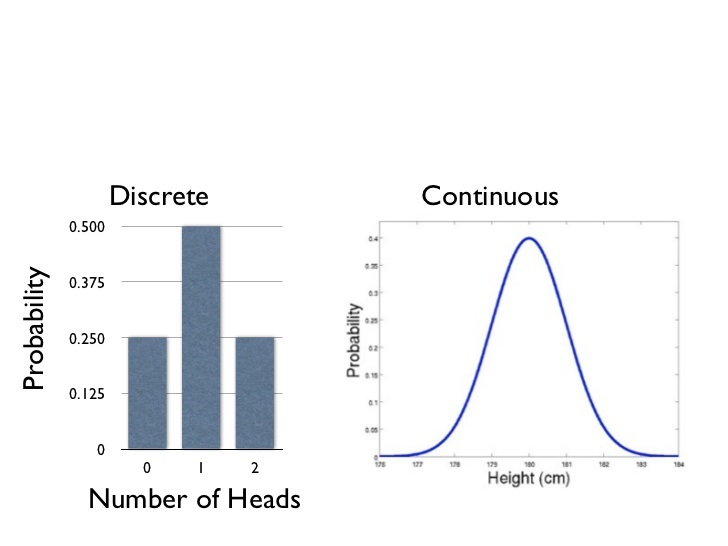
\includegraphics[width=.5\textwidth]{plots/pdfs.jpg}

Discrete Random Variable: Able to compute the possible outcomes, e.g. $u_3$: sum of thrown numbers in 10000 rolls of the dice is discrete, but $u_3$ is almost continuous. For discrete RV we have $\sum_{i=1}^{N} f(u_i) = 1$

Continuous Random Variable: $u_4$: real in interval $[0,1]$. For continuous RV we have $\int_{-\infty}^{\infty} f(u_i)di = 1$, i.e. area under pdf sums to 1.

Expectation of a random variable for $u$: number of one roll of dice:
$$E(u)=\sum_{i=1}^N f(u_i) u_i = \frac{1}{6}(1+2+3+4+5+6) = 3.5$$
weighted average of all possible outcomes (probabilities are weights)

Idea: if we repeat the random experiment an infinite number of times the arithmetic mean will be 3.5 (which will never occur of course).

Variance: measure of dispersion around the expectation
$$var(u) = \sum_{i=1}^{N}f(u_i) (u_i - E(u_i))^2$$
weighted average of quadratic deviations from mean. Note that $f(u_i) = f((u_i-E(u))^2)$ since $E(u)$ deterministic, same probability of occurences, hence variance is also an expectation $$var(u) = E((u-E(u))^2)$$
$\sqrt{var(u)}$ is the standard deviation and has same dimension as u

\paragraph{Conditional and joint probability}
u: number of single roll of dice

v: number of natural numbers through which the trown number of the dice may be divided

\begin{tabular}{c|cccccc}
	\hline 
	RV& \multicolumn{6}{c|}{Outcomes} \\ 
	\hline 
	u& 1 & 2 & 3 & 4 & 5 & 6 \\ 
	\hline 
	v& 1 & 2 & 2 & 3 & 2 & 4 \\ 
	\hline 
\end{tabular} 
Is there a dependence? How do we measure that? Conditional probabilites! Conditional on $v=2$: $Pr(u=3|v=2)=f(u=3|v=2)=1/3$. 2, 3 and 5 are equally likely:
$f(u=1|v=2)=0$
$f(u=2|v=2)=1/3$
$f(u=3|v=2)=1/3$
$f(u=4|v=2)=0$
$f(u=5|v=2)=1/3$
$f(u=6|v=2)=0$

joint distribution: probability distribution for the $N_u N_v = 6\cdot 4=24$ possible outcomes of u and v jointly, hence $f(u,v)$:
\begin{tabular}{|c|c|c|c|c|c|c|c|}
	\hline 
	& \multicolumn{7}{c|}{u} \\ 
	\hline 
	&  & 1 & 2 & 3 & 4 & 5 & 6 \\ 
	\hline 
	& 1 & 1/6 & 0 & 0 & 0 & 0 & 0 \\ 
	\hline 
	v & 2 & 0 & 1/6 & 1/6 & 0 & 1/6 & 0 \\ 
	\hline 
	& 3 & 0 & 0 & 0 & 1/6 & 0 & 0 \\ 
	\hline 
	& 4 & 0 & 0 & 0 & 0 & 0 & 1/6 \\ 
	\hline 
\end{tabular} 
$f(u=3,v=2) = 1/6 = f(u=3|v=2)\cdot f(v=2) = 1/3 \cdot 1/2 = 1/6$
$$f(u,v) = f(u|v) f(v) = f(v|u) f(u)$$

Covariance: idea of positive relationship: if u is rather large, $u-E(u)>>0$, then $v-E(v)>>0$ should also be rather large.
Covariance is a measure for the linear relationship between RV. Look at scatterplot: the better we can put all (u,v) combinations on a straigth line the larger the covariance
$$cov(u,v) = \sum_{i=1}^{N_u}\sum_{j=1}^{N_v} f(u_i,v_j)[(u_i-E(u))(v_j-E(v))]$$
weights according to joint probability
$$cov(u,v) = E[(u-E(u))(v-E(v))]$$
Note that it is always possible (and likely) that there is a nonlinear relationship (study of copulas).

To make covariance independent of units of measure, divide by standard deviations to get correlation:
$$\rho = corr(u,v) = \frac{cov(u,v)}{sd(u)sd(v)}$$
with $-1\leq \rho \leq 1$.

Independence: Random variables that don't have any relationship (neither linear nor nonlinear) are called independent

Example: $u_1$: number on rolled dice 1,$u_2$: number on rolled dice 2, then 
$$f(u_1|u_2) = f(u_1)$$
or 
$$f(u_1,u_2) = f(u_1)f(u_2)=1/36$$

Independence implies a cov=corr=0, but not the other way around.

Rules: Let $u_1$ and $u_2$ be random variables and a,b scalars, then
\begin{align*}
E(b) = b\\
E(b u_1) = b E(u_1)\\
E(u_1+ u_2) = E(u_1) + E(u_2)\\
E(u_1 u_2) \neq E(u_1) E(u_2) \text{Except when independent}\\
E(E(u_1)) = E(u_1) \text{ $E(u)$ is not a random variable}
\end{align*}

$u_3 = a u_1 + b u_2$
$$var(u_3) = a^2 var(u_1) + b^2 var(u_2) + 2 ab cov(u_1,u_2)$$
$u_4 = a+b u_2$
$$var(u_4) = b^2var(u_2)$$
$$cov(u_1,u_2)=cov(u_2,u_1)$$

\paragraph{Probability distributions: Normal distribution}
has bell shape with 2 shape parameters: expectation $\mu$ and variance $\sigma^2$
$$u\sim N(\mu,\sigma^2)$$
$$f(u) = \frac{1}{\sqrt{2\pi var(u)}} exp\{-\frac{1}{2}\frac{(u-E(u))^2}{var(u)}$$


\paragraph{Probability distributions: bivariate normal distribution}
Let $X$ and $Y$ be both  (jointly) normally distributed: $X_i \sim N(\mu_x, \sigma^2_x)$ and $Y_i \sim N(\mu_y, \sigma^2_y)$, $corr(X,Y) = \rho$, then the joint density is
$$f(x,y)=\frac{1}{2\pi\sigma_x\sigma_y(1-\rho^2)}exp\left\{-\frac{-\tilde{x}^2-2\rho\tilde{x}\tilde{y}+\tilde{y}^2}{2(1-\rho)^2}\right\}$$ where $\tilde{x} = (x-\mu_x)/\sigma_x$ and $\tilde{y} = (y-\mu_y)/\sigma_y$.

The conditional expectation is
$$E(Y|X) = \int_{-\infty}^{\infty}\underbrace{\frac{f(X,y)}{f(X)}}_{f(y|X)}y~dy = \left(\mu_y -\mu_x\rho\frac{\sigma_y}{\sigma_x}\right)+\left(\rho \frac{\sigma_y}{\sigma_x}\right) X$$.

The conditional variance is:
$$Var(Y|X) = \int_{-\infty}^{\infty}f(y|X)(y-E(Y|X))^2~dy = \sigma_y^2(1-\rho^2)$$.

What is the distribution of Y conditional on X?
$$Y|X \sim N(\alpha + \beta X, \sigma^2)$$
where $\alpha = \mu_y - \mu_x\rho\frac{\sigma_y}{\sigma_x}$ and $\beta=\rho \frac{\sigma_y}{\sigma_x}$ and $\sigma^2 = \sigma_y^2(1-\rho^2)$. Alternatively:
$Y = \underbrace{\alpha + \beta X}_{E(Y|X)} + u$ with $u\sim N(0,\sigma^2)$.

This is basically what we do with linear regression models.

\paragraph{Empirical counterparts to expectation, variance and correlation}
We now look at the ACTUAL OUTCOME, denote this with small letters $x_1,x_2,...x_T$

Sample mean: $\widehat{E(X)} = \bar{X} = \frac{1}{T} \sum_{t=1}^{T} x_t$ unweighted arithmetic average of realized outcomes. the mean is an unbiased and consistent estimate for the expectation.

Sample variance: $\widehat{var(X)} = S^2 = \frac{1}{T-1} \sum_{t=1}^{T} (x_t -\bar{x})^2 = \frac{1}{T-1} S_{xx}$ we call $S_{xx}$ the variation

Why do we divide by $T-1$ instead of just $T$:

If we divide by $T$ then the estimator is biased. The correction $T/(T-1)$ is called Bessel's correction, it corrects the bias in estimation of the population variance when the population mean is UNKNOWN.

Sample variance is calculated as mean of squared deviations of sample values from sample mean. As the true population mean is unknown, we loose a degree of freedom.

Consider $T=1$: $x_1$ is estimate of expectation, no estimate of variance possible. $T=2$ we may start to make inference about variance.

With T observations, we take only $T-1$ observations to estimate the variance. We need to distinguish population variance
$$\sigma^2 = \sum{i=1}^N \frac{(X_i -\mu)^2}{N}$$
and variance of sample
$$\sigma_t^2 = \sum{i=1}^n \frac{(X_i -\bar{X})^2}{n}$$
Sample variance $S^2$ is an estimator of $\sigma^2$, not $\sigma_t^2$

X deviates from $\bar(X)$ with variance $\sigma_t^2$. Sample mean $\bar{X}$ deviates from $\mu$ with variance $\sigma^2/n$ (sample mean gets different values from sample to sample, it is a random variable with mean $\mu$ and variance $\sigma^2/n$. Roughly: X should deviate from $\mu$ with a variance that includes 2 terms:
$$\sigma^2 = \sigma_t^2 + \frac{\sigma^2}{n} \Leftrightarrow \sigma^2 = \frac{n}{n-1} \sigma_t^2$$

Unbiasedness:

\begin{align*}
E(\bar{X}) = \frac{1}{T} \sum_{t=1}^{T} E(X_t) = \frac{T}{T} \mu = \mu\\
\end{align*}

\begin{align*}
E(S^2) = \frac{1}{T-1} \left(T E(X_t^2) - T E(\bar{X})^2\right)
\end{align*}
with
$$E(X_t^2) = E(X_t)^2 + V(X_t) = \mu^2 + \sigma^2$$
$$E(\bar{X})^2 = \mu^2 + V(\bar{X})$$
$$V(\bar{X}) = V(\frac{1}{T} \sum X_t) = \frac{1}{T^2} \sum(V(X_t)) = \frac{\sigma^2}{T}$$
Hence
\begin{align*}
E(S^2) = \frac{1}{T-1} \left(T (\mu^2 + \sigma^2) - T (\mu^2 + \sigma^2/T)\right) = \frac{T-1}{T-1} \sigma^2 = \sigma^2
\end{align*}
Note: $S^2$ is an unbiased estimator for the variance, but $S$ is a BIASED estimator for the standard deviation!

Sample covariance:
$$\widehat{cov(x,y)} = \frac{1}{T-1}\sum_{t=1}^T (x_t -\bar{x})(y_t - \bar{y}) = \frac{1}{T-1} S_{xy}$$
$S_{xy}$ is a covariation. Sample correlation
$$\widehat{corr(x,y)} = \frac{S_{xy}}{\sqrt{S_{xx}S_{yy}}}$$
\paragraph{Standardization}
$u\sim N(\mu,\sigma^2)$ then $z=\frac{u-\mu}{\sigma} \sim N(0,1)$ with $E(z)=\frac{E(u)-\mu}{\sigma}=0$ and $V(z)=\frac{1}{\sigma^2}var(u) = \frac{\sigma^2}{\sigma^2}=1$
\paragraph{$\chi^2$ distribution}
$$c = z_1^2 + z_2^2 + ... + z_v^2 \sim \chi^2(v)$$
the sum of $v$ independent squared standard normally distributed variables is a $chi^2$ distributed variable with $v$ degrees of freedom. note that $c\geq0$.
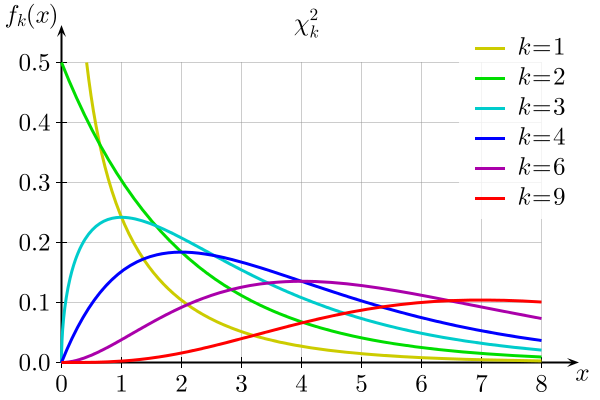
\includegraphics[width=0.5\textwidth]{plots/Chi-square_pdf.png}

For large $v$ it is approximately normal
\paragraph{t-distribution}
$c \sim \chi^2(v)$ and $z\sim N(0,1)$ and $c$ and $z$ are independent, then
$$t=\frac{z}{\sqrt{c/v}} \sim t(v)$$
t-distributed variable with $v$ degrees of freedom. Note that $E(t)=0$ and $V(t)=\frac{v}{v-2}$, $v>2$
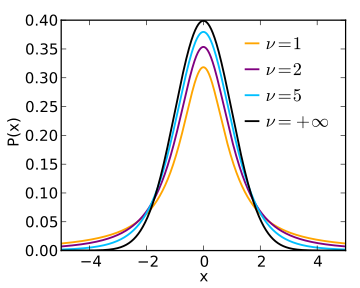
\includegraphics[width=0.5\textwidth]{plots/360px-Student_t_pdf.png}
Very similar to normal distribution, but flatter. for $v>30$ almost no difference

\paragraph{F-distribution}
$c_1 \sim \chi^2(v_1)$ and $c_2 \sim \chi^2(v_2)$ and $c_1$ and $c_2$ independent, then
$$F=\frac{c_1/v_1}{c_2/v_2} = \frac{c_1}{c_2} \frac{v_2}{v_1} \sim F(v_1,v_2)$$, $F>0$
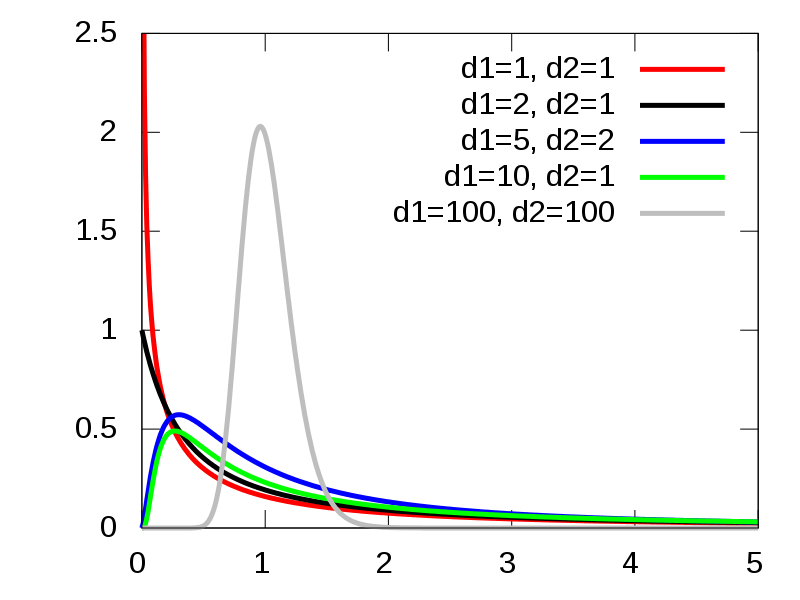
\includegraphics[width=0.5\textwidth]{plots/800px-F-distribution_pdf.png}

\subsection{Specification}

Tip example\marginpar{Slides 20-22}
Example:
Guests of a restaurant leave the waiter with more or less large amounts of tips.Since the waiter is always friendly to all guests he can't explain the difference in tips.  The waiter collects data for 20 guests in a table.

Economic Reasoning: Since the waiter treats all his guests in the same way, it can be assumed that the difference in the amount of gratuities y is essentially declared by the amount of the bill x (measured in euros):

Economic model: functional dependence (in general)
\[ y=f(x) \]
and particularly
\[ y=\alpha +\beta x \]
Focus on linear relationships. Slide with true relationship. $\alpha$ is intercept, $\beta$ is slope of the line. R is the true linear relationship, we want to be as close as possible to it.

Now our work as econometrician begins!
Econometric model:
\[ y_t=\alpha+ \beta x_t+u_t \]
y: endogenous variable, x is exogenous variable, u is error, $\alpha$ and $\beta$ are true coefficients. Even though later on we will study the effects of several variables on another variable, right now we start with the simple linear regression model, i.e. only one exogenous and one endogenous variable. We focus on observed values, hence the subindex $t=1,...,T$, $\alpha$ and $\beta$ are the same for all persons (assumption which we could relax). In Reality we won't see an exact relationship due to randomness, different moods of people, exogenous factors, therefore we add an error term $u$.
Slide with Econometric model.

Side note: Other functional forms are of course possible:
 \begin{itemize}
 	\item Cobb-Douglas Production Function: $Y_t = \alpha L_t^\beta K_t^\gamma e^{u_t}$, take logs, then you get linear form. Of interest: is $\beta+\gamma=1$
 	\item logarithmic: $Y_t = a(X_t)^\beta e^{u_t}$ which may be rewritten $log(Y_t) = log(a) + \beta log(X_t) + u_t$ Then $\beta$ is elasticity:$\beta = \frac{\partial Y_t / Y_t}{\partial X_t / X_t}$ very usefull as this is without dimension:
 	\begin{align*}
 	\frac{\partial log(Y_t)}{\partial log(X_t)} =  	\frac{\partial log(Y_t)}{\partial y_t}  	\frac{\partial Y_t}{\partial X_t}  	\frac{\partial X_t}{\partial log(X_t)} = \frac{1}{Y_t}\partial Y_t \frac{X_t}{\partial X_t} = \frac{\partial Y}{\partial X_t} \frac{X_t}{Y_t} = \beta
 	\end{align*}
 	If $X$ is raised by $1\%$ then $y$ changes by $\beta$ \%.
 	 	\item quadratic (or polynomials)
 	$ Y_t = \alpha + \beta_1 X_t + \beta_2 X_t^2 + u_t$
\end{itemize}
 
 
The econometric model is specified using the A-, B- and  C-assumptions
\paragraph{Functional specification (A-Assumptions)}

\begin{description}
	\item[Assumption a1:] No relevant exogenous variable is omitted from the
	econometric model, and the exogenous variable included in the model is
	relevant [here: what about quality of the meal, we will consider these cases later on]
	
	\item[Assumption a2:] The true functional dependence between $x_{t}$ and $%
	y_{t}$ is linear
	
	\item[Assumption a3:] The parameters $\alpha $ and $\beta $ are constant for
	all $T$ observations $(x_{t},y_{t})$
\end{description}

\paragraph{Error term specification (B-assumptions)}
Why do we need an error term:
\begin{itemize}
	\item unsystematic measurement errors due to proxy variables
	\item some exogenous variables are not considered in the economic model since they are not observable
	\item human behavior is rather unpredictable and humans make errors
\end{itemize}
So the error term is supposed to fluctuate around 0, its average value. u is a random variable. Thougth experiment: Consider an infinite amount of samples of x and therefore y and u. Look at the distribution of u.
\begin{description}
	\item[Assumption b1:] $E(u_{t})=0$ for $t=1,\ldots ,T$ 
	[no systematic measurement errors, very important, we loose efficiency]
	\item[Assumption b2:] Homoskedasticity: $Var(u_{t})=\sigma ^{2}$ for $%
	t=1,\ldots ,T$
	[not so important, we can deal with heteroscedasticity]
	\item[Assumption b3:] For all $t\neq s$ with $t=1,2,...,T$ and $s=1,2,..,T$
	we have%
	\begin{equation*}
	Cov(u_{t},u_{s})=0
	\end{equation*}
	[no autocorrelation, if one persons gives a rather large tip and the person sitting at the next table follows that example, we have autocorrelation, we loose efficiency]
	\item[Assumption b4:] The error terms $u_{t}$ are (jointly) normally distributed.
\end{description}
b1 to b3: white noise assumptions

Compact notation of all B-assumptions: 
\begin{description}
	\item[b1-b4:] $u_{t}\sim NID(0,\sigma ^{2})$ for $t=1,\ldots ,T$
\end{description}\marginpar{Slide 23} 
Actually we have 20 of such distributions. Point A actually observed, u3 residual; expectation of all us must lie on R, have the same variance, bell shaped

\paragraph{Variable specification (C-assumptions)}:

\begin{description}
	\item[Assumption c1] The exogenous variable $x_{t}$ is not stochastic, but
	can be controlled as in an experimental situation
	[highly unlikely, economic data is most often not from experimental situations, we will stick to this due to didactic reasons, later on we discuss what changes if we suppose that x is a random variable but not correlated with u]
	\item[Assumption c2] The exogenous variable $x_{t}$ is not constant for all
	observations $t$: $S_{xx}>0$
	[we need some variation in x to explain the variation in y, this assumption also implies that we need at least two observations (which we also need to estimate two parameters)]
\end{description}

Of course, many (or even all?) of the A-, B-, and C-assumptions are	restrictive and unrealistic	:
\begin{itemize}
	\item Number of exogenous variables, stochastic nature of variables
	\item Dynamics in variables, considering systems of equations
	\item Linear form
	\item Deterministic or stochastic trends
\end{itemize}

We will nevertheless suppose they are satisfied for the time being, and consider their violations later on


\subsection{Point estimation}

The simple (two-variable) linear regression model is
	\begin{equation*}
	y_{t}=\alpha +\beta x_{t}+u_{t}
	\end{equation*}

Estimation: Compute estimated values $\hat{\alpha}$ and $\hat{\beta}$\marginpar{OLS.R}
Intuitively: try to minimize the absolute values of the residuals or alternatively minimize quadratic deviations.

We need to distinguish between true ($\alpha$,$\beta$) and estimated values:
\[ \hat{y}_{t}=\hat{\alpha}+\hat{\beta}x_{t} \]

How can we estimate the coefficients? (values of coefficients)
\paragraph{Least squares method (LS)}
Residual (Residuum): Difference between the observed value $y_{t}$ and the estimated (predicted) value $\hat{y}_{t}$:
\begin{eqnarray*}
	\hat{u}_{t} &=&y_{t}-\hat{y}_{t} \\
	&=&y_{t}-\hat{\alpha}-\hat{\beta}x_{t}
\end{eqnarray*}
Idea: Choose $\hat{\alpha}$ and $\hat{\beta}$ such, that the sum of squared residuals
\[ S_{\hat{u}\hat{u}}=\sum_{t=1}^T \hat{u}_t^2=\sum_{t=1}^T(y_t-\hat\alpha-\hat\beta x_t)^2 \]
is minimized!

\paragraph{Derivation of the OLS estimators}
Necessary conditions: Differentiate - Set FOC to zero - Reorder
Sufficient conditions: Check second-order derivatives

Differentiate%
\[
S_{\hat{u}\hat{u}}=\sum_{t=1}^{T}\left( y_{t}-\hat{\alpha}-\hat{\beta}%
x_{t}\right) ^{2} 
\]%
with respect to $\hat{\alpha}$ and $\hat{\beta}$:%
\begin{eqnarray*}
	\frac{\partial S_{\hat{u}\hat{u}}}{\partial \hat{\alpha}} &=&\sum_{t=1}^{T}2%
	\left( y_{t}-\hat{\alpha}-\hat{\beta}x_{t}\right) \left( -1\right) \\
	\frac{\partial S_{\hat{u}\hat{u}}}{\partial \hat{\beta}} &=&\sum_{t=1}^{T}2%
	\left( y_{t}-\hat{\alpha}-\hat{\beta}x_{t}\right) \left( -x_{t}\right) .
\end{eqnarray*}%
Setting the derivatives to zeros and reordering yields%
\begin{eqnarray*}
	\sum_{t=1}^{T}\left( y_{t}-\hat{\alpha}-\hat{\beta}x_{t}\right) &=&0 \\
	\sum_{t=1}^{T}\left( x_{t}y_{t}-x_{t}\hat{\alpha}-\hat{\beta}%
	x_{t}^{2}\right) &=&0
\end{eqnarray*}%
or the \emph{normal equations }(Normalgleichungen)%
\begin{eqnarray}
\hat{\alpha}T+\hat{\beta}\sum_{t=1}^{T}x_{t} &=&\sum_{t=1}^{T}y_{t}
\label{g1} \\
\hat{\alpha}\sum_{t=1}^{T}x_{t}+\hat{\beta}\sum_{t=1}^{T}x_{t}^{2}
&=&\sum_{t=1}^{T}x_{t}y_{t}.  \label{g2}
\end{eqnarray}%
Different ways to solve this system of equations, e.g. in matrix form:
\begin{align*}
\begin{pmatrix} T & \sum_{t=1}^{T}x_{t}\\ \sum_{t=1}^{T}x_{t} & \sum_{t=1}^{T}x_{t}^2\end{pmatrix} \begin{pmatrix} \hat{\alpha} \\ \hat{\beta} \end{pmatrix} =& \begin{pmatrix} \sum_{t=1}^{T}y_{t}\\ \sum_{t=1}^{T}x_t y_{t}\end{pmatrix}\\
\begin{pmatrix} \hat{\alpha} \\ \hat{\beta} \end{pmatrix} =& \begin{pmatrix} T & \sum_{t=1}^{T}x_{t}\\ \sum_{t=1}^{T}x_{t} & \sum_{t=1}^{T}x_{t}^2\end{pmatrix}^{-1}  \begin{pmatrix} \sum_{t=1}^{T}y_{t}\\ \sum_{t=1}^{T}x_t y_{t}\end{pmatrix}
\end{align*}
Compute the inverse of a $2\times2$ matrix is easy:
\begin{align*}
\begin{pmatrix} T & \sum_{t=1}^{T}x_{t}\\ \sum_{t=1}^{T}x_{t} & \sum_{t=1}^{T}x_{t}^2\end{pmatrix}^{-1} &= \frac{1}{\det\begin{pmatrix} T & \sum_{t=1}^{T}x_{t}\\ \sum_{t=1}^{T}x_{t} & \sum_{t=1}^{T}x_{t}^2\end{pmatrix}} \begin{pmatrix} \sum_{t=1}^{T}x_{t}^2 & -\sum_{t=1}^{T}x_{t}\\ -\sum_{t=1}^{T}x_{t} & T\end{pmatrix}\\
&=\frac{1}{T\sum_{t=1}^{T}x_{t}^{2}-\left( \sum_{t=1}^{T}x_{t}\right) ^{2}} \begin{pmatrix} \sum_{t=1}^{T}x_{t}^2 & -\sum_{t=1}^{T}x_{t}\\ -\sum_{t=1}^{T}x_{t} & T\end{pmatrix}
\end{align*}
Therefore:
\begin{align*}
\begin{pmatrix} \hat{\alpha} \\ \hat{\beta} \end{pmatrix} =& =\frac{1}{T\sum_{t=1}^{T}x_{t}^{2}-\left( \sum_{t=1}^{T}x_{t}\right) ^{2}} \begin{pmatrix} \sum_{t=1}^{T}x_{t}^2 & -\sum_{t=1}^{T}x_{t}\\ -\sum_{t=1}^{T}x_{t} & T\end{pmatrix}  \begin{pmatrix} \sum_{t=1}^{T}y_{t}\\ \sum_{t=1}^{T}x_t y_{t}\end{pmatrix}
\end{align*}
Let's focus on $\hat{\beta}$:
\begin{eqnarray}
\hat{\beta} 
&=&\frac{\sum_{t=1}^{T}x_{t}y_{t}-\frac{1}{T}\sum_{t=1}^{T}x_{t}%
	\sum_{t=1}^{T}y_{t}}{\sum_{t=1}^{T}x_{t}^{2}-\frac{1}{T}\left(
	\sum_{t=1}^{T}x_{t}\right) ^{2}}  \nonumber \\
&=&\frac{\sum_{t=1}^{T}\left( x_{t}-\bar{x}\right) \left( y_{t}-\bar{y}%
	\right) }{\sum_{t=1}^{T}\left( x_{t}-\bar{x}\right) ^{2}}  \nonumber \\
&=&\frac{S_{xy}}{S_{xx}}.  \label{defbetahat}
\end{eqnarray}%

Divide the first normal equation by $T$, then%
\[
\hat{\alpha}+\hat{\beta}\bar{x}=\bar{y} 
\]%
or%
\begin{equation}
\hat{\alpha}=\bar{y}-\hat{\beta}\bar{x}.  \label{defalphahat}
\end{equation}




\begin{eqnarray*}
	\hat{\beta} &=&S_{xy}/S_{xx} \\
	\hat{\alpha} &=&\bar{y}-\hat{\beta}\bar{x}
\end{eqnarray*}%
with 
\begin{eqnarray*}
	S_{xx} &=&\sum \left( x_{t}-\bar{x}\right) ^{2}=\sum x_{t}^{2}-T\bar{x}^{2}
	\\
	S_{xy} &=&\sum \left( x_{t}-\bar{x}\right) \left( y_{t}-\bar{y}\right) =\sum
	y_{t}x_{t}-T\bar{x}\bar{y}
\end{eqnarray*}%
These are variations, not variances or covariances as we are not dividing by $T-1$.

Interpretation of the estimators or estimates? Do for our example! \marginpar{OLS.R}

Numeric illustration for a three points example

\begin{center}%
	\begin{tabular}{|c|c|c|}
		\hline
		$\mathbf{t}$ & $\mathbf{x}_{\mathbf{t}}$ & $\mathbf{y}_{\mathbf{t}}$ \\ 
		\hline
		1 & 10 & 2 \\ 
		2 & 30 & 3 \\ 
		3 & 50 & 7 \\ \hline
	\end{tabular}%
\end{center}%
Calculate
\begin{eqnarray*}
	&&\hat{\alpha},\hat{\beta} \\
	&&\hat{y}_{1},\hat{y}_{2},\hat{y}_{3} \\
	&&\hat{u}_{1},\hat{u}_{2},\hat{u}_{3} \\
	&&S_{\hat{u}}, S_{\hat{u}\hat{u}}
\end{eqnarray*}
Compute $\bar{x}=30$ and $\bar{y}=4$ and%
\begin{eqnarray*}
	S_{xx} &=&\sum \left( x_{t}-\bar{x}\right) ^{2}=400+0+400=800 \\
	S_{xy} &\equiv &\sum \left( x_{t}-\bar{x}\right) \left( y_{t}-\bar{y}\right)
	\\
	&=&(-20)\cdot (-2)+0\cdot 1+20\cdot 3=100
\end{eqnarray*}%
Estimates (Sch\"{a}tzwerte)%
\begin{eqnarray*}
	\hat{\beta} &=&S_{xy}/S_{xx}=100/800=0.125 \\
	\hat{\alpha} &=&\bar{y}-\hat{\beta}\bar{x}=4-0.125\cdot 30=0.25
\end{eqnarray*}%
With each additional Euro on the bill, the waiter receives an additional tip of 0.125 Euro. $\hat{\alpha}$ is a level parameter, mostly no good interpretation (no bill, but still 0.25 Euros tip does not make sense).
Always stick to the interval where you have observations!

Estimated model%
\[
\hat{y}_{t}=0.25+0.125\cdot x_{t} 
\]%
If the billing amounts are $x_{1}=10$, $x_{2}=30$ and $x_{3}=50$ we predict
the following gratuities%
\begin{eqnarray*}
	\hat{y}_{1} &=&0.25+0.125\cdot 10=1.5 \\
	\hat{y}_{2} &=&0.25+0.125\cdot 30=4 \\
	\hat{y}_{3} &=&0.25+0.125\cdot 50=6.5
\end{eqnarray*}%
Estimated error terms (residuals)%
\begin{eqnarray*}
	\hat{u}_{1} &=&y_{1}-\hat{y}_{1}=2-1.5=0.5 \\
	\hat{u}_{2} &=&y_{2}-\hat{y}_{2}=3-4=-1 \\
	\hat{u}_{3} &=&y_{1}-\hat{y}_{1}=7-6.5=0.5
\end{eqnarray*}%
Sum of residuals: $S_{\hat{u}}=0.5-1+0.5=0$. (This is always the case!)

Sum of squared residuals%
\[
S_{\hat{u}\hat{u}}=\sum \hat{u}_{t}^{2}=0.5^{2}+\left( -1\right)
^{2}+0.5^{2}=1.5 
\]


\subsection{The coefficient of determination $R^{2}$}
Variation of the endogenous variable
\[ S_{yy}=S_{\hat{y}\hat{y}}+S_{\hat{u}\hat{u}} \]
$\bar{R}: \bar{y}=\hat{a} + \hat{\beta}\bar{x}$,\\$g:(\bar{x},\bar{y})$
\begin{center}
	%\colorbox{hgrau}{
\unitlength 1mm % = 2.845pt
\linethickness{0.4pt}
\ifx\plotpoint\undefined\newsavebox{\plotpoint}\fi % GNUPLOT compatibility
\begin{picture}(123.9,53)(-10,0)
\put(10,10){\vector(1,0){65}}
\put(10,10){\vector(0,1){35}}
\put(10,10){\line(0,-1){1}}
\put(10,10){\line(-1,0){1}}
\put(9,18){\line(1,0){1}}
\put(9,26){\line(1,0){1}}
\put(10,26){\line(-1,0){1}}
\put(9,34){\line(1,0){1}}
\put(9,42){\line(1,0){1}}
\put(56,28){\line(0,1){0}}
\put(56,28){\line(0,1){0}}
\put(30,9){\line(0,1){1}}
\put(50,9){\line(0,1){1}}
\put(70,9){\line(0,1){1}}
\put(70,6.5){\makebox(0,0)[cc]{\small$60$}}
\put(50,6.5){\makebox(0,0)[cc]{\small$40$}}
\put(30,6.5){\makebox(0,0)[cc]{\small$20$}}
\put(10,6.5){\makebox(0,0)[cc]{\small$0$}}
\put(7.5,10){\makebox(0,0)[rr]{\small$0$}}
\put(7.5,18){\makebox(0,0)[rr]{\small$2$}}
\put(7.5,26){\makebox(0,0)[rr]{\small$4$}}
\put(7.5,34){\makebox(0,0)[rr]{\small$6$}}
\put(7.5,42){\makebox(0,0)[rr]{\small$8$}}
\put(9,47){\small{$y_t$}}
\put(77,9.5){\small{$x_t$}}
%\dashline{1}(40,10)(40,43)
\put(39.93,9.93){\line(0,1){.9706}}
\put(39.93,11.871){\line(0,1){.9706}}
\put(39.93,13.812){\line(0,1){.9706}}
\put(39.93,15.753){\line(0,1){.9706}}
\put(39.93,17.694){\line(0,1){.9706}}
\put(39.93,19.636){\line(0,1){.9706}}
\put(39.93,21.577){\line(0,1){.9706}}
\put(39.93,23.518){\line(0,1){.9706}}
\put(39.93,25.459){\line(0,1){.9706}}
\put(39.93,27.4){\line(0,1){.9706}}
\put(39.93,29.341){\line(0,1){.9706}}
\put(39.93,31.283){\line(0,1){.9706}}
\put(39.93,33.224){\line(0,1){.9706}}
\put(39.93,35.165){\line(0,1){.9706}}
\put(39.93,37.106){\line(0,1){.9706}}
\put(39.93,39.047){\line(0,1){.9706}}
\put(39.93,40.989){\line(0,1){.9706}}
%\end

\thicklines

\put(10,26){\line(1,0){68}}

\thinlines

\put(81,26){\makebox(0,0)[cc]{\small$\overline {R}$}}
\put(37.5,27){\small$g$}

\put(30.0,20.5){\small$|y_1$--\,$\overline{y}|$}
\put(46.0,23){\small$|y_2$--\,$\overline{y}|$}
\put(75.0,31.2){\small$|y_3$--\,$\overline{y}|$}

\put(27.8,21.5){$\scriptscriptstyle\left. \parbox[c][0.8cm][c]{0.1mm}{} \right\rbrace$}
\put(44.0,23.5){$\scriptscriptstyle\left.\parbox[c][0.4cm][c]{0.1mm}{} \right\rbrace $}
\put(72.5,31.3){$\scriptscriptstyle\left.\parbox[c][1.28cm][c]{0.1mm}{} \right\rbrace$}

\put(20,18){\framebox(8,8)[cc]{}}
\put(40,22){\framebox(3.9,3.9)[cc]{}}
\put(60,26){\framebox(12.0,12.0)[cc]{}}

\put(60,38){\circle*{1.5}}
\put(20,18){\circle*{1.5}}
\put(40,26){\circle*{1.5}}
\put(40,22){\circle*{1.5}}

%\dashline{1}(10,26)(20,26)
\put(9.93,25.93){\line(1,0){.9091}}
\put(11.748,25.93){\line(1,0){.9091}}
\put(13.566,25.93){\line(1,0){.9091}}
\put(15.384,25.93){\line(1,0){.9091}}
\put(17.202,25.93){\line(1,0){.9091}}
\put(19.021,25.93){\line(1,0){.9091}}
%\end
%\dashline{1}(28,26)(39,26)
\put(27.93,25.93){\line(1,0){.9167}}
\put(29.763,25.93){\line(1,0){.9167}}
\put(31.596,25.93){\line(1,0){.9167}}
\put(33.43,25.93){\line(1,0){.9167}}
\put(35.263,25.93){\line(1,0){.9167}}
\put(37.096,25.93){\line(1,0){.9167}}
%\end
%\dashline{1}(44,26)(51,26)
\put(43.93,25.93){\line(1,0){.875}}
\put(45.68,25.93){\line(1,0){.875}}
\put(47.43,25.93){\line(1,0){.875}}
\put(49.18,25.93){\line(1,0){.875}}
%\end
\end{picture}
%}
\end{center}
We try to explain the variation in $y_t$ through the variation in $x_t$. $\bar{R}$ is a bad choice since the variation in $y_t$ is equal the variation in $u_t$, but not in $x_t$. $R^{KQ}$ must go through g. We rotate the line such that $S_{\hat{u}\hat{u}}$

\begin{center}
	\unitlength 1mm % = 2.845pt
\linethickness{0.4pt}
\ifx\plotpoint\undefined\newsavebox{\plotpoint}\fi % GNUPLOT compatibility
\begin{picture}(123.9,53)(-12,0)
\put(10,10){\vector(1,0){65}}
\put(10,10){\vector(0,1){35}}
\put(10,10){\line(0,-1){1}}
\put(10,10){\line(-1,0){1}}
\put(9,18){\line(1,0){1}}
\put(9,25.93){\line(1,0){1}}
\put(10,25.93){\line(-1,0){1}}
\put(9,34){\line(1,0){1}}
\put(9,42){\line(1,0){1}}
\put(56,28){\line(0,1){0}}
\put(56,28){\line(0,1){0}}
\put(30,9){\line(0,1){1}}
\put(50,9){\line(0,1){1}}
\put(70,9){\line(0,1){1}}
\put(70,6.5){\makebox(0,0)[cc]{\small$60$}}
\put(50,6.5){\makebox(0,0)[cc]{\small$40$}}
\put(30,6.5){\makebox(0,0)[cc]{\small$20$}}
\put(10,6.5){\makebox(0,0)[cc]{\small$0$}}
\put(7.5,10){\makebox(0,0)[rr]{\small$0$}}
\put(7.5,18){\makebox(0,0)[rr]{\small$2$}}
\put(7.5,26){\makebox(0,0)[rr]{\small$4$}}
\put(7.5,34){\makebox(0,0)[rr]{\small$6$}}
\put(7.5,42){\makebox(0,0)[rr]{\small$8$}}
\put(9,47){\small{$y_t$}}
\put(77,9.5){\small{$x_t$}}

\thicklines
\multiput(10,11)(.06766292135,.03370786517){890}{\line(1,0){.06766292135}}
\thinlines

\put(71,41){\small$\widehat{R}_{KQ}$}
\put(37.5,27){\small$g$}

\put(-9,20.3){\small$|\widehat y_1$--\,$\overline{y}|$}
\put(30.5,18.8){\small$|y_1$--\,$\overline{y}|$}
\put(46.5,23){\small$|y_2$--\,$\overline{y}|$}
\put(36.8,31.1){\small$|\widehat y_3$--\,$\overline{y}|$}
\put(75,31.8){\small$|y_3$--\,$\overline{y}|$}

\put(25,15.8){\small$\widehat u_1$}
\put(30.5,23.5){\small$\widehat u_2$}
\put(52,36.7){\small$\widehat u_3$}

\put(2.3,20.5){$\scriptscriptstyle\left\lbrace \parbox[c][1.05cm][c]{0.1mm}{} \right.$}
\put(22.8,16.9){$\scriptscriptstyle\left. \parbox[c][0.2cm][c]{0.1mm}{} \right\rbrace$}
\put(27,21.9){$\scriptscriptstyle\left. \parbox[c][0.72cm][c]{0.1mm}{} \right\rbrace$}
\put(34,23.5){$\scriptscriptstyle\left\lbrace\parbox[c][0.35cm][c]{0.1mm}{} \right.$}
\put(43.6,23.5){$\scriptscriptstyle\left.\parbox[c][0.35cm][c]{0.1mm}{} \right\rbrace $}
\put(48.1,30.6){$\scriptscriptstyle\left\lbrace \parbox[c][0.9cm][c]{0.1mm}{} \right.$}
\put(55.3,37){$\scriptscriptstyle\left\lbrace\parbox[c][0.2cm][c]{0.1mm}{} \right.$}
\put(72.5,31.9){$\scriptscriptstyle\left.\parbox[c][1.3cm][c]{0.1mm}{} \right\rbrace$}

\put(20,18.8){\framebox(7.05,7.05)[cc]{}}
\put(40,22){\framebox(3.9,3.9)[cc]{}}
\put(60,26){\framebox(12.5,12.5)[cc]{}}

\put(20,17){\fcolorbox{black}{lightgray}{\rule{0.06cm}{0cm}\rule{0cm}{0.06cm}}}
\put(36,23.1){\fcolorbox{black}{lightgray}{\rule{0.17cm}{0cm}\rule{0cm}{0.17cm}}}
\put(57.0,36.9){\fcolorbox{black}{lightgray}{\rule{0.06cm}{0cm}\rule{0cm}{0.06cm}}}

\put(9.98,17.05){\fcolorbox{black}{darkgray}{\rule{0.775cm}{0cm}\rule{0cm}{0.775cm}}}
\put(50,27.05){\fcolorbox{black}{darkgray}{\rule{0.775cm}{0cm}\rule{0cm}{0.775cm}}}

\put(60,38.7){\circle*{1.5}}
\put(20,16){\circle*{1.5}}
\put(60,36){\circle*{1.5}}
\put(40,26){\circle*{1.5}}
\put(20,18.7){\circle*{1.5}}
\put(40,22){\circle*{1.5}}

%\dashline{1}(10,26)(20,26)
\put(9.93,25.93){\line(1,0){.9091}}
\put(11.748,25.93){\line(1,0){.9091}}
\put(13.566,25.93){\line(1,0){.9091}}
\put(15.384,25.93){\line(1,0){.9091}}
\put(17.202,25.93){\line(1,0){.9091}}
\put(19.021,25.93){\line(1,0){.9091}}
%\end
%\dashline{1}(28,26)(39,26)
\put(27.93,25.93){\line(1,0){.9167}}
\put(29.763,25.93){\line(1,0){.9167}}
\put(31.596,25.93){\line(1,0){.9167}}
\put(33.43,25.93){\line(1,0){.9167}}
\put(35.263,25.93){\line(1,0){.9167}}
\put(37.096,25.93){\line(1,0){.9167}}
%\end
%\dashline{1}(44,26)(51,26)
\put(43.93,25.93){\line(1,0){.875}}
\put(45.68,25.93){\line(1,0){.875}}
\put(47.43,25.93){\line(1,0){.875}}
\put(49.18,25.93){\line(1,0){.875}}
%\end
\end{picture}
\end{center}
This shows that the entire variation $S_{yy}$ can be broken down into two components: the explained variation $S_{\hat{y}\hat{y}}$ and the unexplained variation $S_{\hat{u}\hat{u}}$. Graphically, this means that the sum of dark grey and medium grey areas corresponds to the sum of the light grey areas. However, this connection does not apply to a single observation point!

We get the equation:
\[ \sum \left( y_{t}-\bar{y}\right) ^{2}=\sum \left( \hat{y}_{t}-\bar{y}\right)^{2}+\sum \hat{u}_{t}^{2} \]


Proof: Rewrite the normal equations:
\begin{eqnarray*}
\sum_{t=1}^{T}y_{t} &=&\sum_{t=1}^{T}\hat{\alpha}+\hat{\beta}%
\sum_{t=1}^{T}x_{t} \\
\sum_{t=1}^{T}x_{t}y_{t} &=&\hat{\alpha}\sum_{t=1}^{T}x_{t}+\hat{\beta}%
\sum_{t=1}^{T}x_{t}^{2}
\end{eqnarray*}%
or
\begin{eqnarray*}
\sum_{t=1}^{T}y_{t}-\sum_{t=1}^{T}\hat{\alpha}-\hat{\beta}%
\sum_{t=1}^{T}x_{t} &=&0 \\
\sum_{t=1}^{T}x_{t}y_{t}-\hat{\alpha}\sum_{t=1}^{T}x_{t}-\hat{\beta}%
\sum_{t=1}^{T}x_{t}^{2} &=&0
\end{eqnarray*}%
or
\begin{eqnarray*}
\sum_{t=1}^{T}\left( y_{t}-\hat{\alpha}-\hat{\beta}x_{t}\right) &=&0 \\
\sum_{t=1}^{T}x_{t}\left( y_{t}-\hat{\alpha}-\hat{\beta}x_{t}\right) &=&0.
\end{eqnarray*}
Because of $\hat{u}_{t}=y_{t}-\hat{\alpha}-\hat{\beta}x_{t}$ this equals
\begin{eqnarray}
\sum_{t=1}^{T}\hat{u}_{t} &=&0  \label{n1} \\
\sum_{t=1}^{T}x_{t}\hat{u}_{t} &=&0.  \label{n2}
\end{eqnarray}%
The decomposition is now easy to show:
\begin{eqnarray*}
\sum \left( y_{t}-\bar{y}\right) ^{2} &=&\sum \left( y_{t}-\hat{y}_{t}+\hat{y%
}_{t}-\bar{y}\right) ^{2} \\
&=&\sum \hat{u}_{t}^{2}+\sum \left( \hat{y}_{t}-\bar{y}\right) ^{2} \\
&&+\sum 2\hat{u}_{t}\left( \hat{y}_{t}-\bar{y}\right) .
\end{eqnarray*}%
The last term is
\begin{eqnarray*}
\sum 2\hat{u}_{t}\left( \hat{y}_{t}-\bar{y}\right) &=&\sum 2\hat{u}%
_{t}\left( \hat{\alpha}+\hat{\beta}x_{t}-\bar{y}\right) \\
&=&2\hat{\alpha}\sum \hat{u}_{t}+2\hat{\beta}\sum \hat{u}_{t}x_{t}-2\bar{y}%
\sum \hat{u}_{t}.
\end{eqnarray*}%
Due to (\ref{n1}) and (\ref{n2}) this term equals zero. Hence, the decomposition is proved.

Coefficient of determination (Bestimmtheitsmaß) $R^2$
\[ R^{2}=\frac{\text{`explained variation''}}
{\text{``total variation''}}=\frac{S_{yy}-S_{\hat{u}\hat{u}}}{S_{yy}}=\frac{S_{\hat{y}\hat{y}}}{S_{yy}} \]

Different way of computing $R^{2}$:
\[ R^{2}=\frac{\hat{\beta}S_{xy}}{S_{yy}}=\frac{S_{xy}^{2}}{S_{xx}S_{yy}} \]

For our example with the three points:
We already know that%
\begin{eqnarray*}
	S_{xx} &=&\sum \left( x_{t}-\bar{x}\right) ^{2}=800 \\
	S_{xy} &=&\sum \left( x_{t}-\bar{x}\right) \left( y_{t}-\bar{y}\right) =100
\end{eqnarray*}%
Now compute%
\[
S_{yy}=\sum \left( y_{t}-\bar{y}\right) ^{2}=14 
\]%
Calculate%
\begin{eqnarray*}
	R^{2} &=&\frac{S_{xy}^{2}}{S_{xx}S_{yy}} \\
	&=&\frac{100^{2}}{800\cdot 14}\approx 89.3\%
\end{eqnarray*}%
or%
\begin{eqnarray*}
	R^{2} &=&\frac{S_{yy}-S_{\hat{u}\hat{u}}}{S_{yy}} \\
	&=&\frac{14-1.5}{14}\approx 89.3\%
\end{eqnarray*}

Note that in the simple linear regression model: $\widehat{corr}(x,y)=\frac{S_{xy}}{\sqrt{S_{xx}}\sqrt{S_{yy}}}= \pm \sqrt{\frac{S_{xx}^2}{S_{xx}S_{yy}}} = \pm \sqrt{R^2}$

Note also that in models without an intercept the coefficient of determination could be negative.
\section{Properties of the estimators}

The estimates
\begin{eqnarray*}
\hat{\beta} &=&S_{xy}/S_{xx} \\
\hat{\alpha} &=&\bar{y}-\hat{\beta}\bar{x}
\end{eqnarray*}
are random variables.

Thought experiment: repeated samples

Computer simulation \marginpar{experiment.R}

In order to compare different estimators we need criteria for \enquote{good} estimators:
\begin{itemize}
	\item Unbiasedness: An estimator $\hat{\beta}^A$ is unbiased if given an infinite amount of repeated samples, the obtained estimates $\hat{\beta}^A$ are on average equal to the true value of $\beta$, i.e. $E(\hat{\beta}^A)=\beta$.
	\item Efficiency: An estimator $\hat{\beta}^A$ is efficient, if it is the one with the smallest variance $var(\hat{\beta}^A)$ \textbf{within} the class of unbiased estimators.
\end{itemize}
\begin{center}
	\unitlength 1mm % = 2.845pt
\linethickness{0.4pt}
\ifx\plotpoint\undefined\newsavebox{\plotpoint}\fi % GNUPLOT compatibility
\begin{picture}(123.9,47)(0,0)
\put(10,10){\vector(1,0){87}}
\thicklines
\put(14,10){\line(0,1){0}}
\put(14,10){\line(1,0){.66}}
%\emline(14.66,10)(15.32,10.03)
\put(14.66,10){\line(1,0){.66}}
%\end
%\emline(15.32,10.03)(15.96,10.04)
\put(15.32,10.03){\line(1,0){.64}}
%\end
%\emline(15.96,10.04)(16.57,10.08)
\put(15.96,10.04){\line(1,0){.61}}
%\end
%\emline(16.57,10.08)(17.16,10.17)
\put(16.57,10.08){\line(1,0){.59}}
%\end
%\emline(17.16,10.17)(17.77,10.24)
\put(17.16,10.17){\line(1,0){.61}}
%\end
%\emline(17.77,10.24)(18.34,10.33)
\put(17.77,10.24){\line(1,0){.57}}
%\end
%\emline(18.34,10.33)(18.93,10.42)
\put(18.34,10.33){\line(1,0){.59}}
%\end
%\emline(18.93,10.42)(19.5,10.54)
\put(18.93,10.42){\line(1,0){.57}}
%\end
%\emline(19.5,10.54)(20.05,10.67)
\multiput(19.5,10.54)(.1375,.0325){4}{\line(1,0){.1375}}
%\end
%\emline(20.05,10.67)(20.59,10.82)
\multiput(20.05,10.67)(.108,.03){5}{\line(1,0){.108}}
%\end
%\emline(20.59,10.82)(21.11,10.95)
\multiput(20.59,10.82)(.13,.0325){4}{\line(1,0){.13}}
%\end
%\emline(21.11,10.95)(21.64,11.11)
\multiput(21.11,10.95)(.106,.032){5}{\line(1,0){.106}}
%\end
%\emline(21.64,11.11)(22.14,11.28)
\multiput(21.64,11.11)(.083333,.028333){6}{\line(1,0){.083333}}
%\end
%\emline(22.14,11.28)(22.64,11.45)
\multiput(22.14,11.28)(.083333,.028333){6}{\line(1,0){.083333}}
%\end
%\emline(22.64,11.45)(23.14,11.65)
\multiput(22.64,11.45)(.083333,.033333){6}{\line(1,0){.083333}}
%\end
%\emline(23.14,11.65)(23.64,11.86)
\multiput(23.14,11.65)(.071429,.03){7}{\line(1,0){.071429}}
%\end
%\emline(23.64,11.86)(24.09,12.07)
\multiput(23.64,11.86)(.064286,.03){7}{\line(1,0){.064286}}
%\end
%\emline(24.09,12.07)(24.55,12.28)
\multiput(24.09,12.07)(.065714,.03){7}{\line(1,0){.065714}}
%\end
%\emline(24.55,12.28)(25,12.5)
\multiput(24.55,12.28)(.064286,.031429){7}{\line(1,0){.064286}}
%\end
%\emline(25,12.5)(25.46,12.71)
\multiput(25,12.5)(.065714,.03){7}{\line(1,0){.065714}}
%\end
%\emline(25.46,12.71)(25.89,12.96)
\multiput(25.46,12.71)(.05375,.03125){8}{\line(1,0){.05375}}
%\end
%\emline(25.89,12.96)(26.32,13.21)
\multiput(25.89,12.96)(.05375,.03125){8}{\line(1,0){.05375}}
%\end
%\emline(26.32,13.21)(26.73,13.46)
\multiput(26.32,13.21)(.05125,.03125){8}{\line(1,0){.05125}}
%\end
%\emline(26.73,13.46)(27.16,13.75)
\multiput(26.73,13.46)(.047778,.032222){9}{\line(1,0){.047778}}
%\end
%\emline(27.16,13.75)(27.55,14.04)
\multiput(27.16,13.75)(.043333,.032222){9}{\line(1,0){.043333}}
%\end
%\emline(27.55,14.04)(27.93,14.32)
\multiput(27.55,14.04)(.042222,.031111){9}{\line(1,0){.042222}}
%\end
%\emline(27.93,14.32)(28.32,14.61)
\multiput(27.93,14.32)(.043333,.032222){9}{\line(1,0){.043333}}
%\end
%\emline(28.32,14.61)(28.71,14.9)
\multiput(28.32,14.61)(.043333,.032222){9}{\line(1,0){.043333}}
%\end
%\emline(28.71,14.9)(29.07,15.2)
\multiput(28.71,14.9)(.04,.033333){9}{\line(1,0){.04}}
%\end
%\emline(29.07,15.2)(29.41,15.49)
\multiput(29.07,15.2)(.037778,.032222){9}{\line(1,0){.037778}}
%\end
%\emline(29.41,15.49)(29.8,15.79)
\multiput(29.41,15.49)(.043333,.033333){9}{\line(1,0){.043333}}
%\end
%\emline(29.8,15.79)(30.14,16.12)
\multiput(29.8,15.79)(.034,.033){10}{\line(1,0){.034}}
%\end
%\emline(30.14,16.12)(30.48,16.45)
\multiput(30.14,16.12)(.034,.033){10}{\line(1,0){.034}}
%\end
%\emline(30.48,16.45)(30.8,16.78)
\multiput(30.48,16.45)(.032,.033){10}{\line(0,1){.033}}
%\end
%\emline(30.8,16.78)(31.14,17.11)
\multiput(30.8,16.78)(.034,.033){10}{\line(1,0){.034}}
%\end
%\emline(31.14,17.11)(31.46,17.44)
\multiput(31.14,17.11)(.032,.033){10}{\line(0,1){.033}}
%\end
%\emline(31.46,17.44)(31.75,17.77)
\multiput(31.46,17.44)(.032222,.036667){9}{\line(0,1){.036667}}
%\end
%\emline(31.75,17.77)(32.07,18.1)
\multiput(31.75,17.77)(.032,.033){10}{\line(0,1){.033}}
%\end
%\emline(32.07,18.1)(32.32,18.44)
\multiput(32.07,18.1)(.03125,.0425){8}{\line(0,1){.0425}}
%\end
%\emline(32.32,18.44)(32.66,18.77)
\multiput(32.32,18.44)(.034,.033){10}{\line(1,0){.034}}
%\end
%\emline(32.66,18.77)(32.93,19.15)
\multiput(32.66,18.77)(.03,.042222){9}{\line(0,1){.042222}}
%\end
%\emline(32.93,19.15)(33.23,19.49)
\multiput(32.93,19.15)(.033333,.037778){9}{\line(0,1){.037778}}
%\end
%\emline(33.23,19.49)(33.48,19.85)
\multiput(33.23,19.49)(.03125,.045){8}{\line(0,1){.045}}
%\end
%\emline(33.48,19.85)(33.75,20.19)
\multiput(33.48,19.85)(.03,.037778){9}{\line(0,1){.037778}}
%\end
%\emline(33.75,20.19)(34.04,20.57)
\multiput(33.75,20.19)(.032222,.042222){9}{\line(0,1){.042222}}
%\end
%\emline(34.04,20.57)(34.29,20.94)
\multiput(34.04,20.57)(.03125,.04625){8}{\line(0,1){.04625}}
%\end
%\emline(34.29,20.94)(34.55,21.27)
\multiput(34.29,20.94)(.0325,.04125){8}{\line(0,1){.04125}}
%\end
%\emline(34.55,21.27)(34.79,21.65)
\multiput(34.55,21.27)(.03,.0475){8}{\line(0,1){.0475}}
%\end
%\emline(34.79,21.65)(35,21.99)
\multiput(34.79,21.65)(.03,.048571){7}{\line(0,1){.048571}}
%\end
%\emline(35,21.99)(35.25,22.35)
\multiput(35,21.99)(.03125,.045){8}{\line(0,1){.045}}
%\end
%\emline(35.25,22.35)(35.48,22.69)
\multiput(35.25,22.35)(.032857,.048571){7}{\line(0,1){.048571}}
%\end
%\emline(35.48,22.69)(35.73,23.07)
\multiput(35.48,22.69)(.03125,.0475){8}{\line(0,1){.0475}}
%\end
%\emline(35.73,23.07)(35.96,23.44)
\multiput(35.73,23.07)(.032857,.052857){7}{\line(0,1){.052857}}
%\end
%\emline(35.96,23.44)(36.16,23.77)
\multiput(35.96,23.44)(.033333,.055){6}{\line(0,1){.055}}
%\end
%\emline(36.16,23.77)(36.36,24.15)
\multiput(36.16,23.77)(.033333,.063333){6}{\line(0,1){.063333}}
%\end
%\emline(36.36,24.15)(36.57,24.52)
\multiput(36.36,24.15)(.03,.052857){7}{\line(0,1){.052857}}
%\end
%\emline(36.57,24.52)(36.8,24.85)
\multiput(36.57,24.52)(.032857,.047143){7}{\line(0,1){.047143}}
%\end
%\emline(36.8,24.85)(37,25.19)
\multiput(36.8,24.85)(.033333,.056667){6}{\line(0,1){.056667}}
%\end
%\emline(37,25.19)(37.21,25.52)
\multiput(37,25.19)(.03,.047143){7}{\line(0,1){.047143}}
%\end
%\emline(37.21,25.52)(37.41,25.9)
\multiput(37.21,25.52)(.033333,.063333){6}{\line(0,1){.063333}}
%\end
%\emline(37.41,25.9)(37.57,26.19)
\multiput(37.41,25.9)(.032,.058){5}{\line(0,1){.058}}
%\end
%\emline(37.57,26.19)(37.79,26.57)
\multiput(37.57,26.19)(.031429,.054286){7}{\line(0,1){.054286}}
%\end
%\emline(37.79,26.57)(37.98,26.9)
\multiput(37.79,26.57)(.031667,.055){6}{\line(0,1){.055}}
%\end
%\emline(37.98,26.9)(38.16,27.19)
\multiput(37.98,26.9)(.03,.048333){6}{\line(0,1){.048333}}
%\end
%\emline(38.16,27.19)(38.34,27.52)
\multiput(38.16,27.19)(.03,.055){6}{\line(0,1){.055}}
%\end
%\emline(38.34,27.52)(38.54,27.9)
\multiput(38.34,27.52)(.033333,.063333){6}{\line(0,1){.063333}}
%\end
%\emline(38.54,27.9)(38.71,28.19)
\multiput(38.54,27.9)(.028333,.048333){6}{\line(0,1){.048333}}
%\end
%\emline(38.71,28.19)(38.86,28.52)
\multiput(38.71,28.19)(.03,.066){5}{\line(0,1){.066}}
%\end
%\emline(38.86,28.52)(39.05,28.77)
\multiput(38.86,28.52)(.031667,.041667){6}{\line(0,1){.041667}}
%\end
%\emline(39.05,28.77)(39.23,29.1)
\multiput(39.05,28.77)(.03,.055){6}{\line(0,1){.055}}
%\end
%\emline(39.23,29.1)(39.39,29.4)
\multiput(39.23,29.1)(.032,.06){5}{\line(0,1){.06}}
%\end
%\emline(39.39,29.4)(39.57,29.69)
\multiput(39.39,29.4)(.03,.048333){6}{\line(0,1){.048333}}
%\end
%\emline(39.57,29.69)(39.73,29.94)
\multiput(39.57,29.69)(.032,.05){5}{\line(0,1){.05}}
%\end
%\emline(39.73,29.94)(39.89,30.24)
\multiput(39.73,29.94)(.032,.06){5}{\line(0,1){.06}}
%\end
%\emline(39.89,30.24)(40.05,30.52)
\multiput(39.89,30.24)(.032,.056){5}{\line(0,1){.056}}
%\end
%\emline(40.05,30.52)(40.23,30.77)
\multiput(40.05,30.52)(.03,.041667){6}{\line(0,1){.041667}}
%\end
%\emline(40.23,30.77)(40.39,31.02)
\multiput(40.23,30.77)(.032,.05){5}{\line(0,1){.05}}
%\end
%\emline(40.39,31.02)(40.55,31.27)
\multiput(40.39,31.02)(.032,.05){5}{\line(0,1){.05}}
%\end
%\emline(40.55,31.27)(40.71,31.52)
\multiput(40.55,31.27)(.032,.05){5}{\line(0,1){.05}}
%\end
%\emline(40.71,31.52)(40.86,31.69)
\multiput(40.71,31.52)(.03,.034){5}{\line(0,1){.034}}
%\end
%\emline(40.86,31.69)(41.04,31.94)
\multiput(40.86,31.69)(.03,.041667){6}{\line(0,1){.041667}}
%\end
%\emline(41.04,31.94)(41.18,32.16)
\multiput(41.04,31.94)(.028,.044){5}{\line(0,1){.044}}
%\end
%\emline(41.18,32.16)(41.34,32.35)
\multiput(41.18,32.16)(.032,.038){5}{\line(0,1){.038}}
%\end
%\emline(41.34,32.35)(41.5,32.52)
\multiput(41.34,32.35)(.032,.034){5}{\line(0,1){.034}}
%\end
%\emline(41.5,32.52)(41.66,32.69)
\multiput(41.5,32.52)(.032,.034){5}{\line(0,1){.034}}
%\end
%\emline(41.66,32.69)(41.84,32.9)
\multiput(41.66,32.69)(.03,.035){6}{\line(0,1){.035}}
%\end
%\emline(41.84,32.9)(42,33.02)
\multiput(41.84,32.9)(.04,.03){4}{\line(1,0){.04}}
%\end
%\emline(42,33.02)(42.16,33.19)
\multiput(42,33.02)(.032,.034){5}{\line(0,1){.034}}
%\end
%\emline(42.16,33.19)(42.32,33.3)
\put(42.16,33.19){\line(1,0){.16}}
%\end
%\emline(42.32,33.3)(42.48,33.46)
\multiput(42.32,33.3)(.032,.032){5}{\line(0,1){.032}}
%\end
%\emline(42.48,33.46)(42.64,33.55)
\put(42.48,33.46){\line(1,0){.16}}
%\end
%\emline(42.64,33.55)(42.82,33.65)
\put(42.64,33.55){\line(1,0){.18}}
%\end
%\emline(42.82,33.65)(42.98,33.76)
\put(42.82,33.65){\line(1,0){.16}}
%\end
%\emline(42.98,33.76)(43.14,33.8)
\put(42.98,33.76){\line(1,0){.16}}
%\end
%\emline(43.14,33.8)(43.32,33.9)
\put(43.14,33.8){\line(1,0){.18}}
%\end
%\emline(43.32,33.9)(43.5,33.94)
\put(43.32,33.9){\line(1,0){.18}}
%\end
%\emline(43.5,33.94)(43.66,33.98)
\put(43.5,33.94){\line(1,0){.16}}
%\end
\put(43.68,33.99){\line(1,0){.18}}%%%%%%%
\put(43.90,34.01){\line(1,0){.18}}%%%%%%%
\put(44.04,34.01){\line(1,0){.18}}%%%%%
%\end
%\emline(44.18,33.99)(44.36,33.98)
\put(44.18,33.99){\line(1,0){.18}}
%\end
%\emline(44.36,33.98)(44.55,33.94)
\put(44.36,33.98){\line(1,0){.19}}
%\end
%\emline(44.55,33.94)(44.73,33.9)
\put(44.55,33.94){\line(1,0){.18}}
%\end
%\emline(44.73,33.9)(44.89,33.8)
\put(44.73,33.9){\line(1,0){.16}}
%\end
%\emline(44.89,33.8)(45.07,33.76)
\put(44.89,33.8){\line(1,0){.18}}
%\end
%\emline(45.07,33.76)(45.23,33.65)
\put(45.07,33.76){\line(1,0){.16}}
%\end
%\emline(45.23,33.65)(45.39,33.55)
\put(45.23,33.65){\line(1,0){.16}}
%\end
%\emline(45.39,33.55)(45.57,33.46)
\put(45.39,33.55){\line(1,0){.18}}
%\end
%\emline(45.57,33.46)(45.73,33.3)
\multiput(45.57,33.46)(.032,-.032){5}{\line(0,-1){.032}}
%\end
%\emline(45.73,33.3)(45.89,33.19)
\put(45.73,33.3){\line(1,0){.16}}
%\end
%\emline(45.89,33.19)(46.05,33.02)
\multiput(45.89,33.19)(.032,-.034){5}{\line(0,-1){.034}}
%\end
%\emline(46.05,33.02)(46.21,32.9)
\multiput(46.05,33.02)(.04,-.03){4}{\line(1,0){.04}}
%\end
%\emline(46.21,32.9)(46.36,32.69)
\multiput(46.21,32.9)(.03,-.042){5}{\line(0,-1){.042}}
%\end
%\emline(46.36,32.69)(46.54,32.52)
\multiput(46.36,32.69)(.03,-.028333){6}{\line(1,0){.03}}
%\end
%\emline(46.54,32.52)(46.68,32.35)
\multiput(46.54,32.52)(.028,-.034){5}{\line(0,-1){.034}}
%\end
%\emline(46.68,32.35)(46.86,32.16)
\multiput(46.68,32.35)(.03,-.031667){6}{\line(0,-1){.031667}}
%\end
%\emline(46.86,32.16)(47.02,31.94)
\multiput(46.86,32.16)(.032,-.044){5}{\line(0,-1){.044}}
%\end
%\emline(47.02,31.94)(47.18,31.69)
\multiput(47.02,31.94)(.032,-.05){5}{\line(0,-1){.05}}
%\end
%\emline(47.18,31.69)(47.34,31.52)
\multiput(47.18,31.69)(.032,-.034){5}{\line(0,-1){.034}}
%\end
%\emline(47.34,31.52)(47.5,31.27)
\multiput(47.34,31.52)(.032,-.05){5}{\line(0,-1){.05}}
%\end
%\emline(47.5,31.27)(47.66,31.02)
\multiput(47.5,31.27)(.032,-.05){5}{\line(0,-1){.05}}
%\end
%\emline(47.66,31.02)(47.82,30.77)
\multiput(47.66,31.02)(.032,-.05){5}{\line(0,-1){.05}}
%\end
%\emline(47.82,30.77)(47.98,30.52)
\multiput(47.82,30.77)(.032,-.05){5}{\line(0,-1){.05}}
%\end
%\emline(47.98,30.52)(48.14,30.27)
\multiput(47.98,30.52)(.032,-.05){5}{\line(0,-1){.05}}
%\end
%\emline(48.14,30.27)(48.32,29.94)
\multiput(48.14,30.27)(.03,-.055){6}{\line(0,-1){.055}}
%\end
%\emline(48.32,29.94)(48.48,29.69)
\multiput(48.32,29.94)(.032,-.05){5}{\line(0,-1){.05}}
%\end
%\emline(48.48,29.69)(48.64,29.4)
\multiput(48.48,29.69)(.032,-.058){5}{\line(0,-1){.058}}
%\end
%\emline(48.64,29.4)(48.82,29.1)
\multiput(48.64,29.4)(.03,-.05){6}{\line(0,-1){.05}}
%\end
%\emline(48.82,29.1)(48.98,28.77)
\multiput(48.82,29.1)(.032,-.066){5}{\line(0,-1){.066}}
%\end
%\emline(48.98,28.77)(49.16,28.52)
\multiput(48.98,28.77)(.03,-.041667){6}{\line(0,-1){.041667}}
%\end
%\emline(49.16,28.52)(49.34,28.19)
\multiput(49.16,28.52)(.03,-.055){6}{\line(0,-1){.055}}
%\end
%\emline(49.34,28.19)(49.52,27.9)
\multiput(49.34,28.19)(.03,-.048333){6}{\line(0,-1){.048333}}
%\end
%\emline(49.52,27.9)(49.68,27.52)
\multiput(49.52,27.9)(.032,-.076){5}{\line(0,-1){.076}}
%\end
%\emline(49.68,27.52)(49.87,27.19)
\multiput(49.68,27.52)(.031667,-.055){6}{\line(0,-1){.055}}
%\end
%\emline(49.87,27.19)(50.07,26.9)
\multiput(49.87,27.19)(.033333,-.048333){6}{\line(0,-1){.048333}}
%\end
%\emline(50.07,26.9)(50.26,26.57)
\multiput(50.07,26.9)(.031667,-.055){6}{\line(0,-1){.055}}
%\end
%\emline(50.26,26.57)(50.43,26.19)
\multiput(50.26,26.57)(.028333,-.063333){6}{\line(0,-1){.063333}}
%\end
%\emline(50.43,26.19)(50.65,25.9)
\multiput(50.43,26.19)(.031429,-.041429){7}{\line(0,-1){.041429}}
%\end
%\emline(50.65,25.9)(50.83,25.52)
\multiput(50.65,25.9)(.03,-.063333){6}{\line(0,-1){.063333}}
%\end
%\emline(50.83,25.52)(51.04,25.19)
\multiput(50.83,25.52)(.03,-.047143){7}{\line(0,-1){.047143}}
%\end
%\emline(51.04,25.19)(51.26,24.85)
\multiput(51.04,25.19)(.031429,-.048571){7}{\line(0,-1){.048571}}
%\end
%\emline(51.26,24.85)(51.43,24.52)
\multiput(51.26,24.85)(.028333,-.055){6}{\line(0,-1){.055}}
%\end
%\emline(51.43,24.52)(51.65,24.15)
\multiput(51.43,24.52)(.031429,-.052857){7}{\line(0,-1){.052857}}
%\end
%\emline(51.65,24.15)(51.87,23.77)
\multiput(51.65,24.15)(.031429,-.054286){7}{\line(0,-1){.054286}}
%\end
%\emline(51.87,23.77)(52.08,23.44)
\multiput(51.87,23.77)(.03,-.047143){7}{\line(0,-1){.047143}}
%\end
%\emline(52.08,23.44)(52.32,23.07)
\multiput(52.08,23.44)(.03,-.04625){8}{\line(0,-1){.04625}}
%\end
%\emline(52.32,23.07)(52.54,22.69)
\multiput(52.32,23.07)(.031429,-.054286){7}{\line(0,-1){.054286}}
%\end
%\emline(52.54,22.69)(52.79,22.35)
\multiput(52.54,22.69)(.03125,-.0425){8}{\line(0,-1){.0425}}
%\end
%\emline(52.79,22.35)(53.01,22.02)
\multiput(52.79,22.35)(.031429,-.047143){7}{\line(0,-1){.047143}}
%\end
%\emline(53.01,22.02)(53.26,21.65)
\multiput(53.01,22.02)(.03125,-.04625){8}{\line(0,-1){.04625}}
%\end
%\emline(53.26,21.65)(53.51,21.27)
\multiput(53.26,21.65)(.03125,-.0475){8}{\line(0,-1){.0475}}
%\end
%\emline(53.51,21.27)(53.76,20.94)
\multiput(53.51,21.27)(.03125,-.04125){8}{\line(0,-1){.04125}}
%\end
%\emline(53.76,20.94)(54.01,20.57)
\multiput(53.76,20.94)(.03125,-.04625){8}{\line(0,-1){.04625}}
%\end
%\emline(54.01,20.57)(54.29,20.19)
\multiput(54.01,20.57)(.031111,-.042222){9}{\line(0,-1){.042222}}
%\end
%\emline(54.29,20.19)(54.54,19.85)
\multiput(54.29,20.19)(.03125,-.0425){8}{\line(0,-1){.0425}}
%\end
%\emline(54.54,19.85)(54.82,19.49)
\multiput(54.54,19.85)(.031111,-.04){9}{\line(0,-1){.04}}
%\end
%\emline(54.82,19.49)(55.12,19.15)
\multiput(54.82,19.49)(.033333,-.037778){9}{\line(0,-1){.037778}}
%\end
%\emline(55.12,19.15)(55.4,18.77)
\multiput(55.12,19.15)(.031111,-.042222){9}{\line(0,-1){.042222}}
%\end
%\emline(55.4,18.77)(55.68,18.44)
\multiput(55.4,18.77)(.031111,-.036667){9}{\line(0,-1){.036667}}
%\end
%\emline(55.68,18.44)(55.97,18.1)
\multiput(55.68,18.44)(.032222,-.037778){9}{\line(0,-1){.037778}}
%\end
%\emline(55.97,18.1)(56.29,17.77)
\multiput(55.97,18.1)(.032,-.033){10}{\line(0,-1){.033}}
%\end
%\emline(56.29,17.77)(56.58,17.44)
\multiput(56.29,17.77)(.032222,-.036667){9}{\line(0,-1){.036667}}
%\end
%\emline(56.58,17.44)(56.9,17.11)
\multiput(56.58,17.44)(.032,-.033){10}{\line(0,-1){.033}}
%\end
%\emline(56.9,17.11)(57.26,16.78)
\multiput(56.9,17.11)(.036,-.033){10}{\line(1,0){.036}}
%\end
%\emline(57.26,16.78)(57.57,16.45)
\multiput(57.26,16.78)(.031,-.033){10}{\line(0,-1){.033}}
%\end
%\emline(57.57,16.45)(57.9,16.12)
\multiput(57.57,16.45)(.033,-.033){10}{\line(0,-1){.033}}
%\end
%\emline(57.9,16.12)(58.26,15.79)
\multiput(57.9,16.12)(.036,-.033){10}{\line(1,0){.036}}
%\end
%\emline(58.26,15.79)(58.62,15.49)
\multiput(58.26,15.79)(.04,-.033333){9}{\line(1,0){.04}}
%\end
%\emline(58.62,15.49)(58.97,15.2)
\multiput(58.62,15.49)(.038889,-.032222){9}{\line(1,0){.038889}}
%\end
%\emline(58.97,15.2)(59.33,14.9)
\multiput(58.97,15.2)(.04,-.033333){9}{\line(1,0){.04}}
%\end
%\emline(59.33,14.9)(59.71,14.61)
\multiput(59.33,14.9)(.042222,-.032222){9}{\line(1,0){.042222}}
%\end
%\emline(59.71,14.61)(60.12,14.32)
\multiput(59.71,14.61)(.045556,-.032222){9}{\line(1,0){.045556}}
%\end
%\emline(60.12,14.32)(60.51,14.04)
\multiput(60.12,14.32)(.043333,-.031111){9}{\line(1,0){.043333}}
%\end
%\emline(60.51,14.04)(60.9,13.75)
\multiput(60.51,14.04)(.043333,-.032222){9}{\line(1,0){.043333}}
%\end
%\emline(60.9,13.75)(61.29,13.46)
\multiput(60.9,13.75)(.043333,-.032222){9}{\line(1,0){.043333}}
%\end
%\emline(61.29,13.46)(61.72,13.21)
\multiput(61.29,13.46)(.05375,-.03125){8}{\line(1,0){.05375}}
%\end
%\emline(61.72,13.21)(62.15,12.96)
\multiput(61.72,13.21)(.05375,-.03125){8}{\line(1,0){.05375}}
%\end
%\emline(62.15,12.96)(62.58,12.71)
\multiput(62.15,12.96)(.05375,-.03125){8}{\line(1,0){.05375}}
%\end
%\emline(62.58,12.71)(63.04,12.5)
\multiput(62.58,12.71)(.065714,-.03){7}{\line(1,0){.065714}}
%\end
%\emline(63.04,12.5)(63.47,12.28)
\multiput(63.04,12.5)(.061429,-.031429){7}{\line(1,0){.061429}}
%\end
%\emline(63.47,12.28)(63.93,12.07)
\multiput(63.47,12.28)(.065714,-.03){7}{\line(1,0){.065714}}
%\end
%\emline(63.93,12.07)(64.4,11.86)
\multiput(63.93,12.07)(.067143,-.03){7}{\line(1,0){.067143}}
%\end
%\emline(64.4,11.86)(64.9,11.65)
\multiput(64.4,11.86)(.071429,-.03){7}{\line(1,0){.071429}}
%\end
%\emline(64.9,11.65)(65.4,11.45)
\multiput(64.9,11.65)(.083333,-.033333){6}{\line(1,0){.083333}}
%\end
%\emline(65.4,11.45)(65.9,11.28)
\multiput(65.4,11.45)(.083333,-.028333){6}{\line(1,0){.083333}}
%\end
%\emline(65.9,11.28)(66.4,11.11)
\multiput(65.9,11.28)(.083333,-.028333){6}{\line(1,0){.083333}}
%\end
%\emline(66.4,11.11)(66.93,10.95)
\multiput(66.4,11.11)(.106,-.032){5}{\line(1,0){.106}}
%\end
%\emline(66.93,10.95)(67.46,10.82)
\multiput(66.93,10.95)(.1325,-.0325){4}{\line(1,0){.1325}}
%\end
%\emline(67.46,10.82)(68.01,10.67)
\multiput(67.46,10.82)(.11,-.03){5}{\line(1,0){.11}}
%\end
%\emline(68.01,10.67)(68.54,10.54)
\multiput(68.01,10.67)(.1325,-.0325){4}{\line(1,0){.1325}}
%\end
%\emline(68.54,10.54)(69.12,10.42)
\put(68.54,10.54){\line(1,0){.58}}
%\end
%\emline(69.12,10.42)(69.68,10.33)
\put(69.12,10.42){\line(1,0){.56}}
%\end
%\emline(69.68,10.33)(70.29,10.25)
\put(69.68,10.33){\line(1,0){.61}}
%\end
%\emline(70.29,10.25)(70.87,10.17)
\put(70.29,10.25){\line(1,0){.58}}
%\end
%\emline(70.87,10.17)(71.47,10.11)
\put(70.87,10.17){\line(1,0){.6}}
%\end
%\emline(71.47,10.11)(72.08,10.07)
\put(71.47,10.11){\line(1,0){.61}}
%\end
%\emline(72.08,10.07)(72.72,10.03)
\put(72.08,10.07){\line(1,0){.64}}
%\end
%\emline(72.72,10.03)(73.37,10)
\put(72.72,10.03){\line(1,0){.65}}
%\end
\put(73.37,10){\line(1,0){.64}}
\put(74.01,10){\line(1,0){.03}}
\put(30,10){\line(0,1){0}}
\put(30,10){\line(1,0){.66}}
%\emline(30.66,10)(31.32,10.03)
\put(30.66,10){\line(1,0){.66}}
%\end
%\emline(31.32,10.03)(31.96,10.04)
\put(31.32,10.03){\line(1,0){.64}}
%\end
%\emline(31.96,10.04)(32.57,10.08)
\put(31.96,10.04){\line(1,0){.61}}
%\end
%\emline(32.57,10.08)(33.16,10.17)
\put(32.57,10.08){\line(1,0){.59}}
%\end
%\emline(33.16,10.17)(33.77,10.24)
\put(33.16,10.17){\line(1,0){.61}}
%\end
%\emline(33.77,10.24)(34.34,10.33)
\put(33.77,10.24){\line(1,0){.57}}
%\end
%\emline(34.34,10.33)(34.93,10.42)
\put(34.34,10.33){\line(1,0){.59}}
%\end
%\emline(34.93,10.42)(35.5,10.54)
\put(34.93,10.42){\line(1,0){.57}}
%\end
%\emline(35.5,10.54)(36.05,10.67)
\multiput(35.5,10.54)(.1375,.0325){4}{\line(1,0){.1375}}
%\end
%\emline(36.05,10.67)(36.59,10.82)
\multiput(36.05,10.67)(.108,.03){5}{\line(1,0){.108}}
%\end
%\emline(36.59,10.82)(37.11,10.95)
\multiput(36.59,10.82)(.13,.0325){4}{\line(1,0){.13}}
%\end
%\emline(37.11,10.95)(37.64,11.11)
\multiput(37.11,10.95)(.106,.032){5}{\line(1,0){.106}}
%\end
%\emline(37.64,11.11)(38.14,11.28)
\multiput(37.64,11.11)(.083333,.028333){6}{\line(1,0){.083333}}
%\end
%\emline(38.14,11.28)(38.64,11.45)
\multiput(38.14,11.28)(.083333,.028333){6}{\line(1,0){.083333}}
%\end
%\emline(38.64,11.45)(39.14,11.65)
\multiput(38.64,11.45)(.083333,.033333){6}{\line(1,0){.083333}}
%\end
%\emline(39.14,11.65)(39.64,11.86)
\multiput(39.14,11.65)(.071429,.03){7}{\line(1,0){.071429}}
%\end
%\emline(39.64,11.86)(40.09,12.07)
\multiput(39.64,11.86)(.064286,.03){7}{\line(1,0){.064286}}
%\end
%\emline(40.09,12.07)(40.55,12.28)
\multiput(40.09,12.07)(.065714,.03){7}{\line(1,0){.065714}}
%\end
%\emline(40.55,12.28)(41,12.5)
\multiput(40.55,12.28)(.064286,.031429){7}{\line(1,0){.064286}}
%\end
%\emline(41,12.5)(41.46,12.71)
\multiput(41,12.5)(.065714,.03){7}{\line(1,0){.065714}}
%\end
%\emline(41.46,12.71)(41.89,12.96)
\multiput(41.46,12.71)(.05375,.03125){8}{\line(1,0){.05375}}
%\end
%\emline(41.89,12.96)(42.32,13.21)
\multiput(41.89,12.96)(.05375,.03125){8}{\line(1,0){.05375}}
%\end
%\emline(42.32,13.21)(42.73,13.46)
\multiput(42.32,13.21)(.05125,.03125){8}{\line(1,0){.05125}}
%\end
%\emline(42.73,13.46)(43.16,13.75)
\multiput(42.73,13.46)(.047778,.032222){9}{\line(1,0){.047778}}
%\end
%\emline(43.16,13.75)(43.55,14.04)
\multiput(43.16,13.75)(.043333,.032222){9}{\line(1,0){.043333}}
%\end
%\emline(43.55,14.04)(43.93,14.32)
\multiput(43.55,14.04)(.042222,.031111){9}{\line(1,0){.042222}}
%\end
%\emline(43.93,14.32)(44.32,14.61)
\multiput(43.93,14.32)(.043333,.032222){9}{\line(1,0){.043333}}
%\end
%\emline(44.32,14.61)(44.71,14.9)
\multiput(44.32,14.61)(.043333,.032222){9}{\line(1,0){.043333}}
%\end
%\emline(44.71,14.9)(45.07,15.2)
\multiput(44.71,14.9)(.04,.033333){9}{\line(1,0){.04}}
%\end
%\emline(45.07,15.2)(45.41,15.49)
\multiput(45.07,15.2)(.037778,.032222){9}{\line(1,0){.037778}}
%\end
%\emline(45.41,15.49)(45.8,15.79)
\multiput(45.41,15.49)(.043333,.033333){9}{\line(1,0){.043333}}
%\end
%\emline(45.8,15.79)(46.14,16.12)
\multiput(45.8,15.79)(.034,.033){10}{\line(1,0){.034}}
%\end
%\emline(46.14,16.12)(46.48,16.45)
\multiput(46.14,16.12)(.034,.033){10}{\line(1,0){.034}}
%\end
%\emline(46.48,16.45)(46.8,16.78)
\multiput(46.48,16.45)(.032,.033){10}{\line(0,1){.033}}
%\end
%\emline(46.8,16.78)(47.14,17.11)
\multiput(46.8,16.78)(.034,.033){10}{\line(1,0){.034}}
%\end
%\emline(47.14,17.11)(47.46,17.44)
\multiput(47.14,17.11)(.032,.033){10}{\line(0,1){.033}}
%\end
%\emline(47.46,17.44)(47.75,17.77)
\multiput(47.46,17.44)(.032222,.036667){9}{\line(0,1){.036667}}
%\end
%\emline(47.75,17.77)(48.07,18.1)
\multiput(47.75,17.77)(.032,.033){10}{\line(0,1){.033}}
%\end
%\emline(48.07,18.1)(48.32,18.44)
\multiput(48.07,18.1)(.03125,.0425){8}{\line(0,1){.0425}}
%\end
%\emline(48.32,18.44)(48.66,18.77)
\multiput(48.32,18.44)(.034,.033){10}{\line(1,0){.034}}
%\end
%\emline(48.66,18.77)(48.93,19.15)
\multiput(48.66,18.77)(.03,.042222){9}{\line(0,1){.042222}}
%\end
%\emline(48.93,19.15)(49.23,19.49)
\multiput(48.93,19.15)(.033333,.037778){9}{\line(0,1){.037778}}
%\end
%\emline(49.23,19.49)(49.48,19.85)
\multiput(49.23,19.49)(.03125,.045){8}{\line(0,1){.045}}
%\end
%\emline(49.48,19.85)(49.75,20.19)
\multiput(49.48,19.85)(.03,.037778){9}{\line(0,1){.037778}}
%\end
%\emline(49.75,20.19)(50.04,20.57)
\multiput(49.75,20.19)(.032222,.042222){9}{\line(0,1){.042222}}
%\end
%\emline(50.04,20.57)(50.29,20.94)
\multiput(50.04,20.57)(.03125,.04625){8}{\line(0,1){.04625}}
%\end
%\emline(50.29,20.94)(50.54,21.27)
\multiput(50.29,20.94)(.03125,.04125){8}{\line(0,1){.04125}}
%\end
%\emline(50.54,21.27)(50.79,21.65)
\multiput(50.54,21.27)(.03125,.0475){8}{\line(0,1){.0475}}
%\end
%\emline(50.79,21.65)(51,21.99)
\multiput(50.79,21.65)(.03,.048571){7}{\line(0,1){.048571}}
%\end
%\emline(51,21.99)(51.25,22.35)
\multiput(51,21.99)(.03125,.045){8}{\line(0,1){.045}}
%\end
%\emline(51.25,22.35)(51.47,22.69)
\multiput(51.25,22.35)(.031429,.048571){7}{\line(0,1){.048571}}
%\end
%\emline(51.47,22.69)(51.72,23.07)
\multiput(51.47,22.69)(.03125,.0475){8}{\line(0,1){.0475}}
%\end
%\emline(51.72,23.07)(51.96,23.44)
\multiput(51.72,23.07)(.03,.04625){8}{\line(0,1){.04625}}
%\end
%\emline(51.96,23.44)(52.15,23.77)
\multiput(51.96,23.44)(.031667,.055){6}{\line(0,1){.055}}
%\end
%\emline(52.15,23.77)(52.36,24.15)
\multiput(52.15,23.77)(.03,.054286){7}{\line(0,1){.054286}}
%\end
%\emline(52.36,24.15)(52.57,24.52)
\multiput(52.36,24.15)(.03,.052857){7}{\line(0,1){.052857}}
%\end
%\emline(52.57,24.52)(52.79,24.85)
\multiput(52.57,24.52)(.031429,.047143){7}{\line(0,1){.047143}}
%\end
%\emline(52.79,24.85)(53,25.19)
\multiput(52.79,24.85)(.03,.048571){7}{\line(0,1){.048571}}
%\end
%\emline(53,25.19)(53.21,25.52)
\multiput(53,25.19)(.03,.047143){7}{\line(0,1){.047143}}
%\end
%\emline(53.21,25.52)(53.4,25.9)
\multiput(53.21,25.52)(.031667,.063333){6}{\line(0,1){.063333}}
%\end
%\emline(53.4,25.9)(53.57,26.19)
\multiput(53.4,25.9)(.028333,.048333){6}{\line(0,1){.048333}}
%\end
%\emline(53.57,26.19)(53.79,26.57)
\multiput(53.57,26.19)(.031429,.054286){7}{\line(0,1){.054286}}
%\end
%\emline(53.79,26.57)(53.97,26.9)
\multiput(53.79,26.57)(.03,.055){6}{\line(0,1){.055}}
%\end
%\emline(53.97,26.9)(54.15,27.19)
\multiput(53.97,26.9)(.03,.048333){6}{\line(0,1){.048333}}
%\end
%\emline(54.15,27.19)(54.33,27.52)
\multiput(54.15,27.19)(.03,.055){6}{\line(0,1){.055}}
%\end
%\emline(54.33,27.52)(54.54,27.9)
\multiput(54.33,27.52)(.03,.054286){7}{\line(0,1){.054286}}
%\end
%\emline(54.54,27.9)(54.71,28.19)
\multiput(54.54,27.9)(.028333,.048333){6}{\line(0,1){.048333}}
%\end
%\emline(54.71,28.19)(54.86,28.52)
\multiput(54.71,28.19)(.03,.066){5}{\line(0,1){.066}}
%\end
%\emline(54.86,28.52)(55.04,28.77)
\multiput(54.86,28.52)(.03,.041667){6}{\line(0,1){.041667}}
%\end
%\emline(55.04,28.77)(55.22,29.1)
\multiput(55.04,28.77)(.03,.055){6}{\line(0,1){.055}}
%\end
%\emline(55.22,29.1)(55.39,29.4)
\multiput(55.22,29.1)(.028333,.05){6}{\line(0,1){.05}}
%\end
%\emline(55.39,29.4)(55.57,29.69)
\multiput(55.39,29.4)(.03,.048333){6}{\line(0,1){.048333}}
%\end
%\emline(55.57,29.69)(55.72,29.94)
\multiput(55.57,29.69)(.03,.05){5}{\line(0,1){.05}}
%\end
%\emline(55.72,29.94)(55.89,30.24)
\multiput(55.72,29.94)(.028333,.05){6}{\line(0,1){.05}}
%\end
%\emline(55.89,30.24)(56.04,30.52)
\multiput(55.89,30.24)(.03,.056){5}{\line(0,1){.056}}
%\end
%\emline(56.04,30.52)(56.22,30.77)
\multiput(56.04,30.52)(.03,.041667){6}{\line(0,1){.041667}}
%\end
%\emline(56.22,30.77)(56.39,31.02)
\multiput(56.22,30.77)(.028333,.041667){6}{\line(0,1){.041667}}
%\end
%\emline(56.39,31.02)(56.54,31.27)
\multiput(56.39,31.02)(.03,.05){5}{\line(0,1){.05}}
%\end
%\emline(56.54,31.27)(56.71,31.52)
\multiput(56.54,31.27)(.028333,.041667){6}{\line(0,1){.041667}}
%\end
%\emline(56.71,31.52)(56.86,31.69)
\multiput(56.71,31.52)(.03,.034){5}{\line(0,1){.034}}
%\end
%\emline(56.86,31.69)(57.04,31.94)
\multiput(56.86,31.69)(.03,.041667){6}{\line(0,1){.041667}}
%\end
%\emline(57.04,31.94)(57.18,32.16)
\multiput(57.04,31.94)(.028,.044){5}{\line(0,1){.044}}
%\end
%\emline(57.18,32.16)(57.33,32.35)
\multiput(57.18,32.16)(.03,.038){5}{\line(0,1){.038}}
%\end
%\emline(57.33,32.35)(57.5,32.52)
\multiput(57.33,32.35)(.028333,.028333){6}{\line(0,1){.028333}}
%\end
%\emline(57.5,32.52)(57.65,32.69)
\multiput(57.5,32.52)(.03,.034){5}{\line(0,1){.034}}
%\end
%\emline(57.65,32.69)(57.83,32.9)
\multiput(57.65,32.69)(.03,.035){6}{\line(0,1){.035}}
%\end
%\emline(57.83,32.9)(58,33.02)
\multiput(57.83,32.9)(.0425,.03){4}{\line(1,0){.0425}}
%\end
%\emline(58,33.02)(58.15,33.19)
\multiput(58,33.02)(.03,.034){5}{\line(0,1){.034}}
%\end
%\emline(58.15,33.19)(58.32,33.3)
\put(58.15,33.19){\line(1,0){.17}}
%\end
%\emline(58.32,33.3)(58.47,33.46)
\multiput(58.32,33.3)(.03,.032){5}{\line(0,1){.032}}
%\end
%\emline(58.47,33.46)(58.64,33.55)
\put(58.47,33.46){\line(1,0){.17}}
%\end
%\emline(58.64,33.55)(58.82,33.65)
\put(58.64,33.55){\line(1,0){.18}}
%\end
%\emline(58.82,33.65)(58.97,33.76)
\put(58.82,33.65){\line(1,0){.15}}
%\end
%\emline(58.97,33.76)(59.14,33.8)
\put(58.97,33.76){\line(1,0){.17}}
%\end
%\emline(59.14,33.8)(59.32,33.9)
\put(59.14,33.8){\line(1,0){.18}}
%\end
%\emline(59.32,33.9)(59.5,33.94)
\put(59.32,33.9){\line(1,0){.18}}
%\end
%\emline(59.5,33.94)(59.65,33.98)
\put(59.5,33.94){\line(1,0){.18}}
%\end
\put(59.7,33.99){\line(1,0){0.18}}
\put(59.85,34.01){\line(1,0){0.18}}
%\emline(60.04,34.01)(60.18,33.99)
\put(60.04,34.01){\line(1,0){.14}}
%\end
%\emline(60.18,33.99)(60.36,33.98)
\put(60.18,33.99){\line(1,0){.18}}
%\end
%\emline(60.36,33.98)(60.54,33.94)
\put(60.36,33.98){\line(1,0){.18}}
%\end
%\emline(60.54,33.94)(60.72,33.9)
\put(60.54,33.94){\line(1,0){.18}}
%\end
%\emline(60.72,33.9)(60.89,33.8)
\put(60.72,33.9){\line(1,0){.17}}
%\end
%\emline(60.89,33.8)(61.07,33.76)
\put(60.89,33.8){\line(1,0){.18}}
%\end
%\emline(61.07,33.76)(61.22,33.65)
\put(61.07,33.76){\line(1,0){.15}}
%\end
%\emline(61.22,33.65)(61.39,33.55)
\put(61.22,33.65){\line(1,0){.17}}
%\end
%\emline(61.39,33.55)(61.57,33.46)
\put(61.39,33.55){\line(1,0){.18}}
%\end
%\emline(61.57,33.46)(61.72,33.3)
\multiput(61.57,33.46)(.03,-.032){5}{\line(0,-1){.032}}
%\end
%\emline(61.72,33.3)(61.89,33.19)
\put(61.72,33.3){\line(1,0){.17}}
%\end
%\emline(61.89,33.19)(62.04,33.02)
\multiput(61.89,33.19)(.03,-.034){5}{\line(0,-1){.034}}
%\end
%\emline(62.04,33.02)(62.21,32.9)
\multiput(62.04,33.02)(.0425,-.03){4}{\line(1,0){.0425}}
%\end
%\emline(62.21,32.9)(62.36,32.69)
\multiput(62.21,32.9)(.03,-.042){5}{\line(0,-1){.042}}
%\end
%\emline(62.36,32.69)(62.54,32.52)
\multiput(62.36,32.69)(.03,-.028333){6}{\line(1,0){.03}}
%\end
%\emline(62.54,32.52)(62.68,32.35)
\multiput(62.54,32.52)(.028,-.034){5}{\line(0,-1){.034}}
%\end
%\emline(62.68,32.35)(62.86,32.16)
\multiput(62.68,32.35)(.03,-.031667){6}{\line(0,-1){.031667}}
%\end
%\emline(62.86,32.16)(63.01,31.94)
\multiput(62.86,32.16)(.03,-.044){5}{\line(0,-1){.044}}
%\end
%\emline(63.01,31.94)(63.18,31.69)
\multiput(63.01,31.94)(.028333,-.041667){6}{\line(0,-1){.041667}}
%\end
%\emline(63.18,31.69)(63.33,31.52)
\multiput(63.18,31.69)(.03,-.034){5}{\line(0,-1){.034}}
%\end
%\emline(63.33,31.52)(63.5,31.27)
\multiput(63.33,31.52)(.028333,-.041667){6}{\line(0,-1){.041667}}
%\end
%\emline(63.5,31.27)(63.65,31.02)
\multiput(63.5,31.27)(.03,-.05){5}{\line(0,-1){.05}}
%\end
%\emline(63.65,31.02)(63.82,30.77)
\multiput(63.65,31.02)(.028333,-.041667){6}{\line(0,-1){.041667}}
%\end
%\emline(63.82,30.77)(63.97,30.52)
\multiput(63.82,30.77)(.03,-.05){5}{\line(0,-1){.05}}
%\end
%\emline(63.97,30.52)(64.14,30.27)
\multiput(63.97,30.52)(.028333,-.041667){6}{\line(0,-1){.041667}}
%\end
%\emline(64.14,30.27)(64.32,29.94)
\multiput(64.14,30.27)(.03,-.055){6}{\line(0,-1){.055}}
%\end
%\emline(64.32,29.94)(64.47,29.69)
\multiput(64.32,29.94)(.03,-.05){5}{\line(0,-1){.05}}
%\end
%\emline(64.47,29.69)(64.64,29.4)
\multiput(64.47,29.69)(.028333,-.048333){6}{\line(0,-1){.048333}}
%\end
%\emline(64.64,29.4)(64.82,29.1)
\multiput(64.64,29.4)(.03,-.05){6}{\line(0,-1){.05}}
%\end
%\emline(64.82,29.1)(64.97,28.77)
\multiput(64.82,29.1)(.03,-.066){5}{\line(0,-1){.066}}
%\end
%\emline(64.97,28.77)(65.15,28.52)
\multiput(64.97,28.77)(.03,-.041667){6}{\line(0,-1){.041667}}
%\end
%\emline(65.15,28.52)(65.33,28.19)
\multiput(65.15,28.52)(.03,-.055){6}{\line(0,-1){.055}}
%\end
%\emline(65.33,28.19)(65.51,27.9)
\multiput(65.33,28.19)(.03,-.048333){6}{\line(0,-1){.048333}}
%\end
%\emline(65.51,27.9)(65.68,27.52)
\multiput(65.51,27.9)(.028333,-.063333){6}{\line(0,-1){.063333}}
%\end
%\emline(65.68,27.52)(65.87,27.19)
\multiput(65.68,27.52)(.031667,-.055){6}{\line(0,-1){.055}}
%\end
%\emline(65.87,27.19)(66.07,26.9)
\multiput(65.87,27.19)(.033333,-.048333){6}{\line(0,-1){.048333}}
%\end
%\emline(66.07,26.9)(66.26,26.57)
\multiput(66.07,26.9)(.031667,-.055){6}{\line(0,-1){.055}}
%\end
%\emline(66.26,26.57)(66.43,26.19)
\multiput(66.26,26.57)(.028333,-.063333){6}{\line(0,-1){.063333}}
%\end
%\emline(66.43,26.19)(66.65,25.9)
\multiput(66.43,26.19)(.031429,-.041429){7}{\line(0,-1){.041429}}
%\end
%\emline(66.65,25.9)(66.83,25.52)
\multiput(66.65,25.9)(.03,-.063333){6}{\line(0,-1){.063333}}
%\end
%\emline(66.83,25.52)(67.04,25.19)
\multiput(66.83,25.52)(.03,-.047143){7}{\line(0,-1){.047143}}
%\end
%\emline(67.04,25.19)(67.26,24.85)
\multiput(67.04,25.19)(.031429,-.048571){7}{\line(0,-1){.048571}}
%\end
%\emline(67.26,24.85)(67.43,24.52)
\multiput(67.26,24.85)(.028333,-.055){6}{\line(0,-1){.055}}
%\end
%\emline(67.43,24.52)(67.65,24.15)
\multiput(67.43,24.52)(.031429,-.052857){7}{\line(0,-1){.052857}}
%\end
%\emline(67.65,24.15)(67.87,23.77)
\multiput(67.65,24.15)(.031429,-.054286){7}{\line(0,-1){.054286}}
%\end
%\emline(67.87,23.77)(68.08,23.44)
\multiput(67.87,23.77)(.03,-.047143){7}{\line(0,-1){.047143}}
%\end
%\emline(68.08,23.44)(68.32,23.07)
\multiput(68.08,23.44)(.03,-.04625){8}{\line(0,-1){.04625}}
%\end
%\emline(68.32,23.07)(68.54,22.69)
\multiput(68.32,23.07)(.031429,-.054286){7}{\line(0,-1){.054286}}
%\end
%\emline(68.54,22.69)(68.79,22.35)
\multiput(68.54,22.69)(.03125,-.0425){8}{\line(0,-1){.0425}}
%\end
%\emline(68.79,22.35)(69.01,22.02)
\multiput(68.79,22.35)(.031429,-.047143){7}{\line(0,-1){.047143}}
%\end
%\emline(69.01,22.02)(69.26,21.65)
\multiput(69.01,22.02)(.03125,-.04625){8}{\line(0,-1){.04625}}
%\end
%\emline(69.26,21.65)(69.51,21.27)
\multiput(69.26,21.65)(.03125,-.0475){8}{\line(0,-1){.0475}}
%\end
%\emline(69.51,21.27)(69.76,20.94)
\multiput(69.51,21.27)(.03125,-.04125){8}{\line(0,-1){.04125}}
%\end
%\emline(69.76,20.94)(70.01,20.57)
\multiput(69.76,20.94)(.03125,-.04625){8}{\line(0,-1){.04625}}
%\end
%\emline(70.01,20.57)(70.29,20.19)
\multiput(70.01,20.57)(.031111,-.042222){9}{\line(0,-1){.042222}}
%\end
%\emline(70.29,20.19)(70.54,19.85)
\multiput(70.29,20.19)(.03125,-.0425){8}{\line(0,-1){.0425}}
%\end
%\emline(70.54,19.85)(70.82,19.49)
\multiput(70.54,19.85)(.031111,-.04){9}{\line(0,-1){.04}}
%\end
%\emline(70.82,19.49)(71.12,19.15)
\multiput(70.82,19.49)(.033333,-.037778){9}{\line(0,-1){.037778}}
%\end
%\emline(71.12,19.15)(71.4,18.77)
\multiput(71.12,19.15)(.031111,-.042222){9}{\line(0,-1){.042222}}
%\end
%\emline(71.4,18.77)(71.68,18.44)
\multiput(71.4,18.77)(.031111,-.036667){9}{\line(0,-1){.036667}}
%\end
%\emline(71.68,18.44)(71.97,18.1)
\multiput(71.68,18.44)(.032222,-.037778){9}{\line(0,-1){.037778}}
%\end
%\emline(71.97,18.1)(72.29,17.77)
\multiput(71.97,18.1)(.032,-.033){10}{\line(0,-1){.033}}
%\end
%\emline(72.29,17.77)(72.58,17.44)
\multiput(72.29,17.77)(.032222,-.036667){9}{\line(0,-1){.036667}}
%\end
%\emline(72.58,17.44)(72.9,17.11)
\multiput(72.58,17.44)(.032,-.033){10}{\line(0,-1){.033}}
%\end
%\emline(72.9,17.11)(73.26,16.78)
\multiput(72.9,17.11)(.036,-.033){10}{\line(1,0){.036}}
%\end
%\emline(73.26,16.78)(73.57,16.45)
\multiput(73.26,16.78)(.031,-.033){10}{\line(0,-1){.033}}
%\end
%\emline(73.57,16.45)(73.9,16.12)
\multiput(73.57,16.45)(.033,-.033){10}{\line(1,0){.033}}
%\end
%\emline(73.9,16.12)(74.26,15.79)
\multiput(73.9,16.12)(.036,-.033){10}{\line(1,0){.036}}
%\end
%\emline(74.26,15.79)(74.62,15.49)
\multiput(74.26,15.79)(.04,-.033333){9}{\line(1,0){.04}}
%\end
%\emline(74.62,15.49)(74.97,15.2)
\multiput(74.62,15.49)(.038889,-.032222){9}{\line(1,0){.038889}}
%\end
%\emline(74.97,15.2)(75.33,14.9)
\multiput(74.97,15.2)(.04,-.033333){9}{\line(1,0){.04}}
%\end
%\emline(75.33,14.9)(75.71,14.61)
\multiput(75.33,14.9)(.042222,-.032222){9}{\line(1,0){.042222}}
%\end
%\emline(75.71,14.61)(76.12,14.32)
\multiput(75.71,14.61)(.045556,-.032222){9}{\line(1,0){.045556}}
%\end
%\emline(76.12,14.32)(76.51,14.04)
\multiput(76.12,14.32)(.043333,-.031111){9}{\line(1,0){.043333}}
%\end
%\emline(76.51,14.04)(76.9,13.75)
\multiput(76.51,14.04)(.043333,-.032222){9}{\line(1,0){.043333}}
%\end
%\emline(76.9,13.75)(77.29,13.46)
\multiput(76.9,13.75)(.043333,-.032222){9}{\line(1,0){.043333}}
%\end
%\emline(77.29,13.46)(77.72,13.21)
\multiput(77.29,13.46)(.05375,-.03125){8}{\line(1,0){.05375}}
%\end
%\emline(77.72,13.21)(78.15,12.96)
\multiput(77.72,13.21)(.05375,-.03125){8}{\line(1,0){.05375}}
%\end
%\emline(78.15,12.96)(78.58,12.71)
\multiput(78.15,12.96)(.05375,-.03125){8}{\line(1,0){.05375}}
%\end
%\emline(78.58,12.71)(79.04,12.5)
\multiput(78.58,12.71)(.065714,-.03){7}{\line(1,0){.065714}}
%\end
%\emline(79.04,12.5)(79.47,12.28)
\multiput(79.04,12.5)(.061429,-.031429){7}{\line(1,0){.061429}}
%\end
%\emline(79.47,12.28)(79.93,12.07)
\multiput(79.47,12.28)(.065714,-.03){7}{\line(1,0){.065714}}
%\end
%\emline(79.93,12.07)(80.4,11.86)
\multiput(79.93,12.07)(.067143,-.03){7}{\line(1,0){.067143}}
%\end
%\emline(80.4,11.86)(80.9,11.65)
\multiput(80.4,11.86)(.071429,-.03){7}{\line(1,0){.071429}}
%\end
%\emline(80.9,11.65)(81.4,11.45)
\multiput(80.9,11.65)(.083333,-.033333){6}{\line(1,0){.083333}}
%\end
%\emline(81.4,11.45)(81.9,11.28)
\multiput(81.4,11.45)(.083333,-.028333){6}{\line(1,0){.083333}}
%\end
%\emline(81.9,11.28)(82.4,11.11)
\multiput(81.9,11.28)(.083333,-.028333){6}{\line(1,0){.083333}}
%\end
%\emline(82.4,11.11)(82.93,10.95)
\multiput(82.4,11.11)(.106,-.032){5}{\line(1,0){.106}}
%\end
%\emline(82.93,10.95)(83.46,10.82)
\multiput(82.93,10.95)(.1325,-.0325){4}{\line(1,0){.1325}}
%\end
%\emline(83.46,10.82)(84.01,10.67)
\multiput(83.46,10.82)(.11,-.03){5}{\line(1,0){.11}}
%\end
%\emline(84.01,10.67)(84.54,10.54)
\multiput(84.01,10.67)(.1325,-.0325){4}{\line(1,0){.1325}}
%\end
%\emline(84.54,10.54)(85.12,10.42)
\put(84.54,10.54){\line(1,0){.58}}
%\end
%\emline(85.12,10.42)(85.68,10.33)
\put(85.12,10.42){\line(1,0){.56}}
%\end
%\emline(85.68,10.33)(86.29,10.25)
\put(85.68,10.33){\line(1,0){.61}}
%\end
%\emline(86.29,10.25)(86.87,10.17)
\put(86.29,10.25){\line(1,0){.58}}
%\end
%\emline(86.87,10.17)(87.47,10.11)
\put(86.87,10.17){\line(1,0){.6}}
%\end
\thinlines
\put(10,10){\vector(0,1){31}}
%\dottedline(60,33)(60,10)
\multiput(59.93,32.93)(0,-.95833){25}{{\rule{.8pt}{.8pt}}}
%\end
%\dottedline(44,33)(44,10)
\multiput(43.93,32.93)(0,-.95833){25}{{\rule{.8pt}{.8pt}}}
%\end
\put(98,9){$\widehat{\beta}$}
\put(34,5){$E(\widehat{\beta}^A)$=$\beta$}
\put(8,43){$f(\widehat{\beta})$}
\put(57,5){$E(\widehat{\beta}^B)$}
\put(30,32){$f(\widehat{\beta}^A)$}
\put(65,32){$f(\widehat{\beta}^B)$}
\end{picture}\\
		\unitlength 1mm % = 2.845pt
\linethickness{0.4pt}
\ifx\plotpoint\undefined\newsavebox{\plotpoint}\fi % GNUPLOT compatibility
\begin{picture}(123.9,51)(-10,0)
\put(10,9){\vector(0,1){34}}
\put(10,9){\vector(1,0){68}}
\thicklines
%\emline(17.45,10)(18.06,10.07)
\put(17.45,10){\line(1,0){.61}}
%\end
%\emline(18.06,10.07)(18.63,10.16)
\put(18.06,10.07){\line(1,0){.57}}
%\end
%\emline(18.63,10.16)(19.22,10.25)
\put(18.63,10.16){\line(1,0){.59}}
%\end
%\emline(19.22,10.25)(19.79,10.37)
\multiput(19.22,10.25)(.1425,.03){4}{\line(1,0){.1425}}
%\end
%\emline(19.79,10.37)(20.34,10.5)
\multiput(19.79,10.37)(.1375,.0325){4}{\line(1,0){.1375}}
%\end
%\emline(20.34,10.5)(20.88,10.65)
\multiput(20.34,10.5)(.108,.03){5}{\line(1,0){.108}}
%\end
%\emline(20.88,10.65)(21.4,10.78)
\multiput(20.88,10.65)(.13,.0325){4}{\line(1,0){.13}}
%\end
%\emline(21.4,10.78)(21.93,10.94)
\multiput(21.4,10.78)(.106,.032){5}{\line(1,0){.106}}
%\end
%\emline(21.93,10.94)(22.43,11.11)
\multiput(21.93,10.94)(.083333,.028333){6}{\line(1,0){.083333}}
%\end
%\emline(22.43,11.11)(22.93,11.28)
\multiput(22.43,11.11)(.083333,.028333){6}{\line(1,0){.083333}}
%\end
%\emline(22.93,11.28)(23.43,11.48)
\multiput(22.93,11.28)(.083333,.033333){6}{\line(1,0){.083333}}
%\end
%\emline(23.43,11.48)(23.93,11.69)
\multiput(23.43,11.48)(.071429,.03){7}{\line(1,0){.071429}}
%\end
%\emline(23.93,11.69)(24.38,11.9)
\multiput(23.93,11.69)(.064286,.03){7}{\line(1,0){.064286}}
%\end
%\emline(24.38,11.9)(24.84,12.11)
\multiput(24.38,11.9)(.065714,.03){7}{\line(1,0){.065714}}
%\end
%\emline(24.84,12.11)(25.29,12.33)
\multiput(24.84,12.11)(.064286,.031429){7}{\line(1,0){.064286}}
%\end
%\emline(25.29,12.33)(25.75,12.54)
\multiput(25.29,12.33)(.065714,.03){7}{\line(1,0){.065714}}
%\end
%\emline(25.75,12.54)(26.18,12.79)
\multiput(25.75,12.54)(.05375,.03125){8}{\line(1,0){.05375}}
%\end
%\emline(26.18,12.79)(26.61,13.04)
\multiput(26.18,12.79)(.05375,.03125){8}{\line(1,0){.05375}}
%\end
%\emline(26.61,13.04)(27.02,13.29)
\multiput(26.61,13.04)(.05125,.03125){8}{\line(1,0){.05125}}
%\end
%\emline(27.02,13.29)(27.45,13.58)
\multiput(27.02,13.29)(.047778,.032222){9}{\line(1,0){.047778}}
%\end
%\emline(27.45,13.58)(27.84,13.87)
\multiput(27.45,13.58)(.043333,.032222){9}{\line(1,0){.043333}}
%\end
%\emline(27.84,13.87)(28.22,14.15)
\multiput(27.84,13.87)(.042222,.031111){9}{\line(1,0){.042222}}
%\end
%\emline(28.22,14.15)(28.61,14.44)
\multiput(28.22,14.15)(.043333,.032222){9}{\line(1,0){.043333}}
%\end
%\emline(28.61,14.44)(29,14.73)
\multiput(28.61,14.44)(.043333,.032222){9}{\line(1,0){.043333}}
%\end
%\emline(29,14.73)(29.36,15.03)
\multiput(29,14.73)(.04,.033333){9}{\line(1,0){.04}}
%\end
%\emline(29.36,15.03)(29.7,15.32)
\multiput(29.36,15.03)(.037778,.032222){9}{\line(1,0){.037778}}
%\end
%\emline(29.7,15.32)(30.09,15.62)
\multiput(29.7,15.32)(.043333,.033333){9}{\line(1,0){.043333}}
%\end
%\emline(30.09,15.62)(30.43,15.95)
\multiput(30.09,15.62)(.034,.033){10}{\line(1,0){.034}}
%\end
%\emline(30.43,15.95)(30.77,16.28)
\multiput(30.43,15.95)(.034,.033){10}{\line(1,0){.034}}
%\end
%\emline(30.77,16.28)(31.09,16.61)
\multiput(30.77,16.28)(.032,.033){10}{\line(0,1){.033}}
%\end
%\emline(31.09,16.61)(31.43,16.94)
\multiput(31.09,16.61)(.034,.033){10}{\line(1,0){.034}}
%\end
%\emline(31.43,16.94)(31.75,17.27)
\multiput(31.43,16.94)(.032,.033){10}{\line(0,1){.033}}
%\end
%\emline(31.75,17.27)(32.04,17.6)
\multiput(31.75,17.27)(.032222,.036667){9}{\line(0,1){.036667}}
%\end
%\emline(32.04,17.6)(32.36,17.93)
\multiput(32.04,17.6)(.032,.033){10}{\line(0,1){.033}}
%\end
%\emline(32.36,17.93)(32.61,18.27)
\multiput(32.36,17.93)(.03125,.0425){8}{\line(0,1){.0425}}
%\end
%\emline(32.61,18.27)(32.95,18.6)
\multiput(32.61,18.27)(.034,.033){10}{\line(1,0){.034}}
%\end
%\emline(32.95,18.6)(33.22,18.98)
\multiput(32.95,18.6)(.03,.042222){9}{\line(0,1){.042222}}
%\end
%\emline(33.22,18.98)(33.52,19.32)
\multiput(33.22,18.98)(.033333,.037778){9}{\line(0,1){.037778}}
%\end
%\emline(33.52,19.32)(33.77,19.68)
\multiput(33.52,19.32)(.03125,.045){8}{\line(0,1){.045}}
%\end
%\emline(33.77,19.68)(34.04,20.02)
\multiput(33.77,19.68)(.03,.037778){9}{\line(0,1){.037778}}
%\end
%\emline(34.04,20.02)(34.33,20.4)
\multiput(34.04,20.02)(.032222,.042222){9}{\line(0,1){.042222}}
%\end
%\emline(34.33,20.4)(34.58,20.77)
\multiput(34.33,20.4)(.03125,.04625){8}{\line(0,1){.04625}}
%\end
%\emline(34.58,20.77)(34.84,21.1)
\multiput(34.58,20.77)(.0325,.04125){8}{\line(0,1){.04125}}
%\end
%\emline(34.84,21.1)(35.08,21.48)
\multiput(34.84,21.1)(.03,.0475){8}{\line(0,1){.0475}}
%\end
%\emline(35.08,21.48)(35.29,21.82)
\multiput(35.08,21.48)(.03,.048571){7}{\line(0,1){.048571}}
%\end
%\emline(35.29,21.82)(35.54,22.18)
\multiput(35.29,21.82)(.03125,.045){8}{\line(0,1){.045}}
%\end
%\emline(35.54,22.18)(35.77,22.52)
\multiput(35.54,22.18)(.032857,.048571){7}{\line(0,1){.048571}}
%\end
%\emline(35.77,22.52)(36.02,22.9)
\multiput(35.77,22.52)(.03125,.0475){8}{\line(0,1){.0475}}
%\end
%\emline(36.02,22.9)(36.25,23.27)
\multiput(36.02,22.9)(.032857,.052857){7}{\line(0,1){.052857}}
%\end
%\emline(36.25,23.27)(36.45,23.6)
\multiput(36.25,23.27)(.033333,.055){6}{\line(0,1){.055}}
%\end
%\emline(36.45,23.6)(36.65,23.98)
\multiput(36.45,23.6)(.033333,.063333){6}{\line(0,1){.063333}}
%\end
%\emline(36.65,23.98)(36.86,24.35)
\multiput(36.65,23.98)(.03,.052857){7}{\line(0,1){.052857}}
%\end
%\emline(36.86,24.35)(37.09,24.68)
\multiput(36.86,24.35)(.032857,.047143){7}{\line(0,1){.047143}}
%\end
%\emline(37.09,24.68)(37.29,25.02)
\multiput(37.09,24.68)(.033333,.056667){6}{\line(0,1){.056667}}
%\end
%\emline(37.29,25.02)(37.5,25.35)
\multiput(37.29,25.02)(.03,.047143){7}{\line(0,1){.047143}}
%\end
%\emline(37.5,25.35)(37.7,25.73)
\multiput(37.5,25.35)(.033333,.063333){6}{\line(0,1){.063333}}
%\end
%\emline(37.7,25.73)(37.86,26.02)
\multiput(37.7,25.73)(.032,.058){5}{\line(0,1){.058}}
%\end
%\emline(37.86,26.02)(38.08,26.4)
\multiput(37.86,26.02)(.031429,.054286){7}{\line(0,1){.054286}}
%\end
%\emline(38.08,26.4)(38.27,26.73)
\multiput(38.08,26.4)(.031667,.055){6}{\line(0,1){.055}}
%\end
%\emline(38.27,26.73)(38.45,27.02)
\multiput(38.27,26.73)(.03,.048333){6}{\line(0,1){.048333}}
%\end
%\emline(38.45,27.02)(38.63,27.35)
\multiput(38.45,27.02)(.03,.055){6}{\line(0,1){.055}}
%\end
%\emline(38.63,27.35)(38.83,27.73)
\multiput(38.63,27.35)(.033333,.063333){6}{\line(0,1){.063333}}
%\end
%\emline(38.83,27.73)(39,28.02)
\multiput(38.83,27.73)(.028333,.048333){6}{\line(0,1){.048333}}
%\end
%\emline(39,28.02)(39.15,28.35)
\multiput(39,28.02)(.03,.066){5}{\line(0,1){.066}}
%\end
%\emline(39.15,28.35)(39.34,28.6)
\multiput(39.15,28.35)(.031667,.041667){6}{\line(0,1){.041667}}
%\end
%\emline(39.34,28.6)(39.52,28.93)
\multiput(39.34,28.6)(.03,.055){6}{\line(0,1){.055}}
%\end
%\emline(39.52,28.93)(39.68,29.23)
\multiput(39.52,28.93)(.032,.06){5}{\line(0,1){.06}}
%\end
%\emline(39.68,29.23)(39.86,29.52)
\multiput(39.68,29.23)(.03,.048333){6}{\line(0,1){.048333}}
%\end
%\emline(39.86,29.52)(40.02,29.77)
\multiput(39.86,29.52)(.032,.05){5}{\line(0,1){.05}}
%\end
%\emline(40.02,29.77)(40.18,30.07)
\multiput(40.02,29.77)(.032,.06){5}{\line(0,1){.06}}
%\end
%\emline(40.18,30.07)(40.34,30.35)
\multiput(40.18,30.07)(.032,.056){5}{\line(0,1){.056}}
%\end
%\emline(40.34,30.35)(40.52,30.6)
\multiput(40.34,30.35)(.03,.041667){6}{\line(0,1){.041667}}
%\end
%\emline(40.52,30.6)(40.68,30.85)
\multiput(40.52,30.6)(.032,.05){5}{\line(0,1){.05}}
%\end
%\emline(40.68,30.85)(40.84,31.1)
\multiput(40.68,30.85)(.032,.05){5}{\line(0,1){.05}}
%\end
%\emline(40.84,31.1)(41,31.35)
\multiput(40.84,31.1)(.032,.05){5}{\line(0,1){.05}}
%\end
%\emline(41,31.35)(41.15,31.52)
\multiput(41,31.35)(.03,.034){5}{\line(0,1){.034}}
%\end
%\emline(41.15,31.52)(41.33,31.77)
\multiput(41.15,31.52)(.03,.041667){6}{\line(0,1){.041667}}
%\end
%\emline(41.33,31.77)(41.47,31.99)
\multiput(41.33,31.77)(.028,.044){5}{\line(0,1){.044}}
%\end
%\emline(41.47,31.99)(41.63,32.18)
\multiput(41.47,31.99)(.032,.038){5}{\line(0,1){.038}}
%\end
%\emline(41.63,32.18)(41.79,32.35)
\multiput(41.63,32.18)(.032,.034){5}{\line(0,1){.034}}
%\end
%\emline(41.79,32.35)(41.95,32.52)
\multiput(41.79,32.35)(.032,.034){5}{\line(0,1){.034}}
%\end
%\emline(41.95,32.52)(42.13,32.73)
\multiput(41.95,32.52)(.03,.035){6}{\line(0,1){.035}}
%\end
%\emline(42.13,32.73)(42.29,32.85)
\put(42.13,32.73){\line(1,0){.16}}
%\end
%\emline(42.29,32.85)(42.45,33.02)
\multiput(42.29,32.85)(.032,.034){5}{\line(0,1){.034}}
%\end
%\emline(42.45,33.02)(42.61,33.13)
\put(42.45,33.02){\line(1,0){.16}}
%\end
%\emline(42.61,33.13)(42.77,33.29)
\multiput(42.61,33.13)(.032,.032){5}{\line(0,1){.032}}
%\end
%\emline(42.77,33.29)(42.93,33.38)
\put(42.77,33.29){\line(1,0){.16}}
%\end
%\emline(42.93,33.38)(43.11,33.48)
\put(42.93,33.38){\line(1,0){.18}}
%\end
%\emline(43.11,33.48)(43.27,33.59)
\put(43.11,33.48){\line(1,0){.16}}
%\end
%\emline(43.27,33.59)(43.43,33.63)
\put(43.27,33.59){\line(1,0){.16}}
%\end
%\emline(43.43,33.63)(43.61,33.73)
\put(43.43,33.63){\line(1,0){.18}}
%\end
%\emline(43.61,33.73)(43.79,33.77)
\put(43.61,33.73){\line(1,0){.18}}
%\end
%\emline(43.79,33.77)(43.95,33.81)
\put(43.79,33.77){\line(1,0){.16}}
%\end
\put(43.95,33.80){\line(1,0){0.18}}
\put(44.15,33.82){\line(1,0){0.18}}
%\emline(44.33,33.84)(44.47,33.82)
\put(44.33,33.84){\line(1,0){.14}}
%\end
%\emline(44.47,33.82)(44.65,33.81)
\put(44.47,33.82){\line(1,0){.18}}
%\end
%\emline(44.65,33.81)(44.84,33.77)
\put(44.65,33.81){\line(1,0){.19}}
%\end
%\emline(44.84,33.77)(45.02,33.73)
\put(44.84,33.77){\line(1,0){.18}}
%\end
%\emline(45.02,33.73)(45.18,33.63)
\put(45.02,33.73){\line(1,0){.16}}
%\end
%\emline(45.18,33.63)(45.36,33.59)
\put(45.18,33.63){\line(1,0){.18}}
%\end
%\emline(45.36,33.59)(45.52,33.48)
\put(45.36,33.59){\line(1,0){.16}}
%\end
%\emline(45.52,33.48)(45.68,33.38)
\put(45.52,33.48){\line(1,0){.16}}
%\end
%\emline(45.68,33.38)(45.86,33.29)
\put(45.68,33.38){\line(1,0){.18}}
%\end
%\emline(45.86,33.29)(46.02,33.13)
\multiput(45.86,33.29)(.032,-.032){5}{\line(0,-1){.032}}
%\end
%\emline(46.02,33.13)(46.18,33.02)
\put(46.02,33.13){\line(1,0){.16}}
%\end
%\emline(46.18,33.02)(46.34,32.85)
\multiput(46.18,33.02)(.032,-.034){5}{\line(0,-1){.034}}
%\end
%\emline(46.34,32.85)(46.5,32.73)
\put(46.34,32.85){\line(1,0){.16}}
%\end
%\emline(46.5,32.73)(46.65,32.52)
\multiput(46.5,32.73)(.03,-.042){5}{\line(0,-1){.042}}
%\end
%\emline(46.65,32.52)(46.83,32.35)
\multiput(46.65,32.52)(.03,-.028333){6}{\line(1,0){.03}}
%\end
%\emline(46.83,32.35)(46.97,32.18)
\multiput(46.83,32.35)(.028,-.034){5}{\line(0,-1){.034}}
%\end
%\emline(46.97,32.18)(47.15,31.99)
\multiput(46.97,32.18)(.03,-.031667){6}{\line(0,-1){.031667}}
%\end
%\emline(47.15,31.99)(47.31,31.77)
\multiput(47.15,31.99)(.032,-.044){5}{\line(0,-1){.044}}
%\end
%\emline(47.31,31.77)(47.47,31.52)
\multiput(47.31,31.77)(.032,-.05){5}{\line(0,-1){.05}}
%\end
%\emline(47.47,31.52)(47.63,31.35)
\multiput(47.47,31.52)(.032,-.034){5}{\line(0,-1){.034}}
%\end
%\emline(47.63,31.35)(47.79,31.1)
\multiput(47.63,31.35)(.032,-.05){5}{\line(0,-1){.05}}
%\end
%\emline(47.79,31.1)(47.95,30.85)
\multiput(47.79,31.1)(.032,-.05){5}{\line(0,-1){.05}}
%\end
%\emline(47.95,30.85)(48.11,30.6)
\multiput(47.95,30.85)(.032,-.05){5}{\line(0,-1){.05}}
%\end
%\emline(48.11,30.6)(48.27,30.35)
\multiput(48.11,30.6)(.032,-.05){5}{\line(0,-1){.05}}
%\end
%\emline(48.27,30.35)(48.43,30.1)
\multiput(48.27,30.35)(.032,-.05){5}{\line(0,-1){.05}}
%\end
%\emline(48.43,30.1)(48.61,29.77)
\multiput(48.43,30.1)(.03,-.055){6}{\line(0,-1){.055}}
%\end
%\emline(48.61,29.77)(48.77,29.52)
\multiput(48.61,29.77)(.032,-.05){5}{\line(0,-1){.05}}
%\end
%\emline(48.77,29.52)(48.93,29.23)
\multiput(48.77,29.52)(.032,-.058){5}{\line(0,-1){.058}}
%\end
%\emline(48.93,29.23)(49.11,28.93)
\multiput(48.93,29.23)(.03,-.05){6}{\line(0,-1){.05}}
%\end
%\emline(49.11,28.93)(49.27,28.6)
\multiput(49.11,28.93)(.032,-.066){5}{\line(0,-1){.066}}
%\end
%\emline(49.27,28.6)(49.45,28.35)
\multiput(49.27,28.6)(.03,-.041667){6}{\line(0,-1){.041667}}
%\end
%\emline(49.45,28.35)(49.63,28.02)
\multiput(49.45,28.35)(.03,-.055){6}{\line(0,-1){.055}}
%\end
%\emline(49.63,28.02)(49.81,27.73)
\multiput(49.63,28.02)(.03,-.048333){6}{\line(0,-1){.048333}}
%\end
%\emline(49.81,27.73)(49.97,27.35)
\multiput(49.81,27.73)(.032,-.076){5}{\line(0,-1){.076}}
%\end
%\emline(49.97,27.35)(50.16,27.02)
\multiput(49.97,27.35)(.031667,-.055){6}{\line(0,-1){.055}}
%\end
%\emline(50.16,27.02)(50.36,26.73)
\multiput(50.16,27.02)(.033333,-.048333){6}{\line(0,-1){.048333}}
%\end
%\emline(50.36,26.73)(50.55,26.4)
\multiput(50.36,26.73)(.031667,-.055){6}{\line(0,-1){.055}}
%\end
%\emline(50.55,26.4)(50.72,26.02)
\multiput(50.55,26.4)(.028333,-.063333){6}{\line(0,-1){.063333}}
%\end
%\emline(50.72,26.02)(50.94,25.73)
\multiput(50.72,26.02)(.031429,-.041429){7}{\line(0,-1){.041429}}
%\end
%\emline(50.94,25.73)(51.12,25.35)
\multiput(50.94,25.73)(.03,-.063333){6}{\line(0,-1){.063333}}
%\end
%\emline(51.12,25.35)(51.33,25.02)
\multiput(51.12,25.35)(.03,-.047143){7}{\line(0,-1){.047143}}
%\end
%\emline(51.33,25.02)(51.55,24.68)
\multiput(51.33,25.02)(.031429,-.048571){7}{\line(0,-1){.048571}}
%\end
%\emline(51.55,24.68)(51.72,24.35)
\multiput(51.55,24.68)(.028333,-.055){6}{\line(0,-1){.055}}
%\end
%\emline(51.72,24.35)(51.94,23.98)
\multiput(51.72,24.35)(.031429,-.052857){7}{\line(0,-1){.052857}}
%\end
%\emline(51.94,23.98)(52.16,23.6)
\multiput(51.94,23.98)(.031429,-.054286){7}{\line(0,-1){.054286}}
%\end
%\emline(52.16,23.6)(52.37,23.27)
\multiput(52.16,23.6)(.03,-.047143){7}{\line(0,-1){.047143}}
%\end
%\emline(52.37,23.27)(52.61,22.9)
\multiput(52.37,23.27)(.03,-.04625){8}{\line(0,-1){.04625}}
%\end
%\emline(52.61,22.9)(52.83,22.52)
\multiput(52.61,22.9)(.031429,-.054286){7}{\line(0,-1){.054286}}
%\end
%\emline(52.83,22.52)(53.08,22.18)
\multiput(52.83,22.52)(.03125,-.0425){8}{\line(0,-1){.0425}}
%\end
%\emline(53.08,22.18)(53.3,21.85)
\multiput(53.08,22.18)(.031429,-.047143){7}{\line(0,-1){.047143}}
%\end
%\emline(53.3,21.85)(53.55,21.48)
\multiput(53.3,21.85)(.03125,-.04625){8}{\line(0,-1){.04625}}
%\end
%\emline(53.55,21.48)(53.8,21.1)
\multiput(53.55,21.48)(.03125,-.0475){8}{\line(0,-1){.0475}}
%\end
%\emline(53.8,21.1)(54.05,20.77)
\multiput(53.8,21.1)(.03125,-.04125){8}{\line(0,-1){.04125}}
%\end
%\emline(54.05,20.77)(54.3,20.4)
\multiput(54.05,20.77)(.03125,-.04625){8}{\line(0,-1){.04625}}
%\end
%\emline(54.3,20.4)(54.58,20.02)
\multiput(54.3,20.4)(.031111,-.042222){9}{\line(0,-1){.042222}}
%\end
%\emline(54.58,20.02)(54.83,19.68)
\multiput(54.58,20.02)(.03125,-.0425){8}{\line(0,-1){.0425}}
%\end
%\emline(54.83,19.68)(55.11,19.32)
\multiput(54.83,19.68)(.031111,-.04){9}{\line(0,-1){.04}}
%\end
%\emline(55.11,19.32)(55.41,18.98)
\multiput(55.11,19.32)(.033333,-.037778){9}{\line(0,-1){.037778}}
%\end
%\emline(55.41,18.98)(55.69,18.6)
\multiput(55.41,18.98)(.031111,-.042222){9}{\line(0,-1){.042222}}
%\end
%\emline(55.69,18.6)(55.97,18.27)
\multiput(55.69,18.6)(.031111,-.036667){9}{\line(0,-1){.036667}}
%\end
%\emline(55.97,18.27)(56.26,17.93)
\multiput(55.97,18.27)(.032222,-.037778){9}{\line(0,-1){.037778}}
%\end
%\emline(56.26,17.93)(56.58,17.6)
\multiput(56.26,17.93)(.032,-.033){10}{\line(0,-1){.033}}
%\end
%\emline(56.58,17.6)(56.87,17.27)
\multiput(56.58,17.6)(.032222,-.036667){9}{\line(0,-1){.036667}}
%\end
%\emline(56.87,17.27)(57.19,16.94)
\multiput(56.87,17.27)(.032,-.033){10}{\line(0,-1){.033}}
%\end
%\emline(57.19,16.94)(57.55,16.61)
\multiput(57.19,16.94)(.036,-.033){10}{\line(1,0){.036}}
%\end
%\emline(57.55,16.61)(57.86,16.28)
\multiput(57.55,16.61)(.031,-.033){10}{\line(0,-1){.033}}
%\end
%\emline(57.86,16.28)(58.19,15.95)
\multiput(57.86,16.28)(.033,-.033){10}{\line(1,0){.033}}
%\end
%\emline(58.19,15.95)(58.55,15.62)
\multiput(58.19,15.95)(.036,-.033){10}{\line(1,0){.036}}
%\end
%\emline(58.55,15.62)(58.91,15.32)
\multiput(58.55,15.62)(.04,-.033333){9}{\line(1,0){.04}}
%\end
%\emline(58.91,15.32)(59.26,15.03)
\multiput(58.91,15.32)(.038889,-.032222){9}{\line(1,0){.038889}}
%\end
%\emline(59.26,15.03)(59.62,14.73)
\multiput(59.26,15.03)(.04,-.033333){9}{\line(1,0){.04}}
%\end
%\emline(59.62,14.73)(60,14.44)
\multiput(59.62,14.73)(.042222,-.032222){9}{\line(1,0){.042222}}
%\end
%\emline(60,14.44)(60.41,14.15)
\multiput(60,14.44)(.045556,-.032222){9}{\line(1,0){.045556}}
%\end
%\emline(60.41,14.15)(60.8,13.87)
\multiput(60.41,14.15)(.043333,-.031111){9}{\line(1,0){.043333}}
%\end
%\emline(60.8,13.87)(61.19,13.58)
\multiput(60.8,13.87)(.043333,-.032222){9}{\line(1,0){.043333}}
%\end
%\emline(61.19,13.58)(61.58,13.29)
\multiput(61.19,13.58)(.043333,-.032222){9}{\line(1,0){.043333}}
%\end
%\emline(61.58,13.29)(62.01,13.04)
\multiput(61.58,13.29)(.05375,-.03125){8}{\line(1,0){.05375}}
%\end
%\emline(62.01,13.04)(62.44,12.79)
\multiput(62.01,13.04)(.05375,-.03125){8}{\line(1,0){.05375}}
%\end
%\emline(62.44,12.79)(62.87,12.54)
\multiput(62.44,12.79)(.05375,-.03125){8}{\line(1,0){.05375}}
%\end
%\emline(62.87,12.54)(63.33,12.33)
\multiput(62.87,12.54)(.065714,-.03){7}{\line(1,0){.065714}}
%\end
%\emline(63.33,12.33)(63.76,12.11)
\multiput(63.33,12.33)(.061429,-.031429){7}{\line(1,0){.061429}}
%\end
%\emline(63.76,12.11)(64.22,11.9)
\multiput(63.76,12.11)(.065714,-.03){7}{\line(1,0){.065714}}
%\end
%\emline(64.22,11.9)(64.69,11.69)
\multiput(64.22,11.9)(.067143,-.03){7}{\line(1,0){.067143}}
%\end
%\emline(64.69,11.69)(65.19,11.48)
\multiput(64.69,11.69)(.071429,-.03){7}{\line(1,0){.071429}}
%\end
%\emline(65.19,11.48)(65.69,11.28)
\multiput(65.19,11.48)(.083333,-.033333){6}{\line(1,0){.083333}}
%\end
%\emline(65.69,11.28)(66.19,11.11)
\multiput(65.69,11.28)(.083333,-.028333){6}{\line(1,0){.083333}}
%\end
%\emline(66.19,11.11)(66.69,10.94)
\multiput(66.19,11.11)(.083333,-.028333){6}{\line(1,0){.083333}}
%\end
%\emline(66.69,10.94)(67.22,10.78)
\multiput(66.69,10.94)(.106,-.032){5}{\line(1,0){.106}}
%\end
%\emline(67.22,10.78)(67.75,10.65)
\multiput(67.22,10.78)(.1325,-.0325){4}{\line(1,0){.1325}}
%\end
%\emline(67.75,10.65)(68.3,10.5)
\multiput(67.75,10.65)(.11,-.03){5}{\line(1,0){.11}}
%\end
%\emline(68.3,10.5)(68.83,10.37)
\multiput(68.3,10.5)(.1325,-.0325){4}{\line(1,0){.1325}}
%\end
%\emline(68.83,10.37)(69.41,10.25)
\multiput(68.83,10.37)(.145,-.03){4}{\line(1,0){.145}}
%\end
%\emline(69.41,10.25)(69.97,10.16)
\put(69.41,10.25){\line(1,0){.56}}
%\end
%\emline(69.97,10.16)(70.58,10.08)
\put(69.97,10.16){\line(1,0){.61}}
%\end
%\emline(70.58,10.08)(71.16,10)
\put(70.58,10.08){\line(1,0){.58}}
%\end
\put(14,10.98){\line(0,1){0}}
%\emline(14,10.98)(14.46,11.04)
\put(14,10.98){\line(1,0){.46}}
%\end
%\emline(14.46,11.04)(14.94,11.11)
\put(14.46,11.04){\line(1,0){.48}}
%\end
%\emline(14.94,11.11)(15.39,11.17)
\put(14.94,11.11){\line(1,0){.45}}
%\end
%\emline(15.39,11.17)(15.85,11.25)
\put(15.39,11.17){\line(1,0){.46}}
%\end
%\emline(15.85,11.25)(16.29,11.34)
\put(15.85,11.25){\line(1,0){.44}}
%\end
%\emline(16.29,11.34)(16.72,11.44)
\put(16.29,11.34){\line(1,0){.43}}
%\end
%\emline(16.72,11.44)(17.15,11.53)
\put(16.72,11.44){\line(1,0){.43}}
%\end
%\emline(17.15,11.53)(17.57,11.63)
\put(17.15,11.53){\line(1,0){.42}}
%\end
%\emline(17.57,11.63)(17.98,11.74)
\put(17.57,11.63){\line(1,0){.41}}
%\end
%\emline(17.98,11.74)(18.4,11.84)
\put(17.98,11.74){\line(1,0){.42}}
%\end
%\emline(18.4,11.84)(18.79,11.96)
\multiput(18.4,11.84)(.0975,.03){4}{\line(1,0){.0975}}
%\end
%\emline(18.79,11.96)(19.18,12.08)
\put(18.79,11.96){\line(1,0){.39}}
%\end
%\emline(19.18,12.08)(19.58,12.2)
\put(19.18,12.08){\line(1,0){.4}}
%\end
%\emline(19.58,12.2)(19.95,12.33)
\multiput(19.58,12.2)(.0925,.0325){4}{\line(1,0){.0925}}
%\end
%\emline(19.95,12.33)(20.33,12.48)
\multiput(19.95,12.33)(.076,.03){5}{\line(1,0){.076}}
%\end
%\emline(20.33,12.48)(20.7,12.61)
\multiput(20.33,12.48)(.0925,.0325){4}{\line(1,0){.0925}}
%\end
%\emline(20.7,12.61)(21.06,12.75)
\multiput(20.7,12.61)(.072,.028){5}{\line(1,0){.072}}
%\end
%\emline(21.06,12.75)(21.4,12.9)
\multiput(21.06,12.75)(.068,.03){5}{\line(1,0){.068}}
%\end
%\emline(21.4,12.9)(21.75,13.04)
\multiput(21.4,12.9)(.07,.028){5}{\line(1,0){.07}}
%\end
%\emline(21.75,13.04)(22.11,13.2)
\multiput(21.75,13.04)(.072,.032){5}{\line(1,0){.072}}
%\end
%\emline(22.11,13.2)(22.45,13.34)
\multiput(22.11,13.2)(.068,.028){5}{\line(1,0){.068}}
%\end
%\emline(22.45,13.34)(22.77,13.5)
\multiput(22.45,13.34)(.064,.032){5}{\line(1,0){.064}}
%\end
%\emline(22.77,13.5)(23.11,13.66)
\multiput(22.77,13.5)(.068,.032){5}{\line(1,0){.068}}
%\end
%\emline(23.11,13.66)(23.43,13.83)
\multiput(23.11,13.66)(.053333,.028333){6}{\line(1,0){.053333}}
%\end
%\emline(23.43,13.83)(23.75,14)
\multiput(23.43,13.83)(.053333,.028333){6}{\line(1,0){.053333}}
%\end
%\emline(23.75,14)(24.06,14.17)
\multiput(23.75,14)(.051667,.028333){6}{\line(1,0){.051667}}
%\end
%\emline(24.06,14.17)(24.36,14.34)
\multiput(24.06,14.17)(.05,.028333){6}{\line(1,0){.05}}
%\end
%\emline(24.36,14.34)(24.66,14.51)
\multiput(24.36,14.34)(.05,.028333){6}{\line(1,0){.05}}
%\end
%\emline(24.66,14.51)(24.97,14.7)
\multiput(24.66,14.51)(.051667,.031667){6}{\line(1,0){.051667}}
%\end
%\emline(24.97,14.7)(25.25,14.87)
\multiput(24.97,14.7)(.046667,.028333){6}{\line(1,0){.046667}}
%\end
%\emline(25.25,14.87)(25.54,15.05)
\multiput(25.25,14.87)(.048333,.03){6}{\line(1,0){.048333}}
%\end
%\emline(25.54,15.05)(25.84,15.25)
\multiput(25.54,15.05)(.05,.033333){6}{\line(1,0){.05}}
%\end
%\emline(25.84,15.25)(26.11,15.42)
\multiput(25.84,15.25)(.045,.028333){6}{\line(1,0){.045}}
%\end
%\emline(26.11,15.42)(26.4,15.62)
\multiput(26.11,15.42)(.048333,.033333){6}{\line(1,0){.048333}}
%\end
%\emline(26.4,15.62)(26.68,15.8)
\multiput(26.4,15.62)(.046667,.03){6}{\line(1,0){.046667}}
%\end
%\emline(26.68,15.8)(26.95,16)
\multiput(26.68,15.8)(.045,.033333){6}{\line(1,0){.045}}
%\end
%\emline(26.95,16)(27.22,16.19)
\multiput(26.95,16)(.045,.031667){6}{\line(1,0){.045}}
%\end
%\emline(27.22,16.19)(27.49,16.37)
\multiput(27.22,16.19)(.045,.03){6}{\line(1,0){.045}}
%\end
%\emline(27.49,16.37)(27.75,16.57)
\multiput(27.49,16.37)(.043333,.033333){6}{\line(1,0){.043333}}
%\end
%\emline(27.75,16.57)(28,16.76)
\multiput(27.75,16.57)(.041667,.031667){6}{\line(1,0){.041667}}
%\end
%\emline(28,16.76)(28.27,16.95)
\multiput(28,16.76)(.045,.031667){6}{\line(1,0){.045}}
%\end
%\emline(28.27,16.95)(28.52,17.16)
\multiput(28.27,16.95)(.035714,.03){7}{\line(1,0){.035714}}
%\end
%\emline(28.52,17.16)(28.77,17.35)
\multiput(28.52,17.16)(.041667,.031667){6}{\line(1,0){.041667}}
%\end
%\emline(28.77,17.35)(29.02,17.54)
\multiput(28.77,17.35)(.041667,.031667){6}{\line(1,0){.041667}}
%\end
%\emline(29.02,17.54)(29.27,17.75)
\multiput(29.02,17.54)(.035714,.03){7}{\line(1,0){.035714}}
%\end
%\emline(29.27,17.75)(29.52,17.93)
\multiput(29.27,17.75)(.041667,.03){6}{\line(1,0){.041667}}
%\end
%\emline(29.52,17.93)(29.77,18.13)
\multiput(29.52,17.93)(.041667,.033333){6}{\line(1,0){.041667}}
%\end
%\emline(29.77,18.13)(30,18.33)
\multiput(29.77,18.13)(.038333,.033333){6}{\line(1,0){.038333}}
%\end
%\emline(30,18.33)(30.25,18.52)
\multiput(30,18.33)(.041667,.031667){6}{\line(1,0){.041667}}
%\end
%\emline(30.25,18.52)(30.49,18.71)
\multiput(30.25,18.52)(.04,.031667){6}{\line(1,0){.04}}
%\end
%\emline(30.49,18.71)(30.72,18.92)
\multiput(30.49,18.71)(.032857,.03){7}{\line(1,0){.032857}}
%\end
%\emline(30.72,18.92)(30.97,19.1)
\multiput(30.72,18.92)(.041667,.03){6}{\line(1,0){.041667}}
%\end
%\emline(30.97,19.1)(31.2,19.3)
\multiput(30.97,19.1)(.038333,.033333){6}{\line(1,0){.038333}}
%\end
%\emline(31.2,19.3)(31.45,19.5)
\multiput(31.2,19.3)(.041667,.033333){6}{\line(1,0){.041667}}
%\end
%\emline(31.45,19.5)(31.68,19.68)
\multiput(31.45,19.5)(.038333,.03){6}{\line(1,0){.038333}}
%\end
%\emline(31.68,19.68)(31.91,19.87)
\multiput(31.68,19.68)(.038333,.031667){6}{\line(1,0){.038333}}
%\end
%\emline(31.91,19.87)(32.15,20.07)
\multiput(31.91,19.87)(.04,.033333){6}{\line(1,0){.04}}
%\end
%\emline(32.15,20.07)(32.38,20.25)
\multiput(32.15,20.07)(.038333,.03){6}{\line(1,0){.038333}}
%\end
%\emline(32.38,20.25)(32.61,20.43)
\multiput(32.38,20.25)(.038333,.03){6}{\line(1,0){.038333}}
%\end
%\emline(32.61,20.43)(32.86,20.61)
\multiput(32.61,20.43)(.041667,.03){6}{\line(1,0){.041667}}
%\end
%\emline(32.86,20.61)(33.09,20.79)
\multiput(32.86,20.61)(.038333,.03){6}{\line(1,0){.038333}}
%\end
%\emline(33.09,20.79)(33.33,20.98)
\multiput(33.09,20.79)(.04,.031667){6}{\line(1,0){.04}}
%\end
%\emline(33.33,20.98)(33.56,21.16)
\multiput(33.33,20.98)(.038333,.03){6}{\line(1,0){.038333}}
%\end
%\emline(33.56,21.16)(33.79,21.34)
\multiput(33.56,21.16)(.038333,.03){6}{\line(1,0){.038333}}
%\end
%\emline(33.79,21.34)(34.04,21.51)
\multiput(33.79,21.34)(.041667,.028333){6}{\line(1,0){.041667}}
%\end
%\emline(34.04,21.51)(34.27,21.68)
\multiput(34.04,21.51)(.038333,.028333){6}{\line(1,0){.038333}}
%\end
%\emline(34.27,21.68)(34.52,21.85)
\multiput(34.27,21.68)(.041667,.028333){6}{\line(1,0){.041667}}
%\end
%\emline(34.52,21.85)(34.75,22.01)
\multiput(34.52,21.85)(.046,.032){5}{\line(1,0){.046}}
%\end
%\emline(34.75,22.01)(35,22.17)
\multiput(34.75,22.01)(.05,.032){5}{\line(1,0){.05}}
%\end
%\emline(35,22.17)(35.25,22.33)
\multiput(35,22.17)(.05,.032){5}{\line(1,0){.05}}
%\end
%\emline(35.25,22.33)(35.49,22.48)
\multiput(35.25,22.33)(.048,.03){5}{\line(1,0){.048}}
%\end
%\emline(35.49,22.48)(35.74,22.63)
\multiput(35.49,22.48)(.05,.03){5}{\line(1,0){.05}}
%\end
%\emline(35.74,22.63)(35.99,22.77)
\multiput(35.74,22.63)(.05,.028){5}{\line(1,0){.05}}
%\end
%\emline(35.99,22.77)(36.24,22.93)
\multiput(35.99,22.77)(.05,.032){5}{\line(1,0){.05}}
%\end
%\emline(36.24,22.93)(36.49,23.07)
\multiput(36.24,22.93)(.05,.028){5}{\line(1,0){.05}}
%\end
%\emline(36.49,23.07)(36.75,23.2)
\multiput(36.49,23.07)(.065,.0325){4}{\line(1,0){.065}}
%\end
%\emline(36.75,23.2)(37,23.34)
\multiput(36.75,23.2)(.05,.028){5}{\line(1,0){.05}}
%\end
%\emline(37,23.34)(37.27,23.46)
\put(37,23.34){\line(1,0){.27}}
%\end
%\emline(37.27,23.46)(37.54,23.59)
\multiput(37.27,23.46)(.0675,.0325){4}{\line(1,0){.0675}}
%\end
%\emline(37.54,23.59)(37.79,23.7)
\put(37.54,23.59){\line(1,0){.25}}
%\end
%\emline(37.79,23.7)(38.06,23.83)
\multiput(37.79,23.7)(.0675,.0325){4}{\line(1,0){.0675}}
%\end
%\emline(38.06,23.83)(38.34,23.93)
\put(38.06,23.83){\line(1,0){.28}}
%\end
%\emline(38.34,23.93)(38.61,24.03)
\put(38.34,23.93){\line(1,0){.27}}
%\end
%\emline(38.61,24.03)(38.9,24.13)
\put(38.61,24.03){\line(1,0){.29}}
%\end
%\emline(38.9,24.13)(39.18,24.24)
\put(38.9,24.13){\line(1,0){.28}}
%\end
%\emline(39.18,24.24)(39.47,24.33)
\put(39.18,24.24){\line(1,0){.29}}
%\end
%\emline(39.47,24.33)(39.77,24.41)
\put(39.47,24.33){\line(1,0){.3}}
%\end
%\emline(39.77,24.41)(40.06,24.49)
\put(39.77,24.41){\line(1,0){.29}}
%\end
%\emline(40.06,24.49)(40.36,24.57)
\put(40.06,24.49){\line(1,0){.3}}
%\end
%\emline(40.36,24.57)(40.66,24.63)
\put(40.36,24.57){\line(1,0){.3}}
%\end
%\emline(40.66,24.63)(40.97,24.69)
\put(40.66,24.63){\line(1,0){.31}}
%\end
%\emline(40.97,24.69)(41.29,24.76)
\put(40.97,24.69){\line(1,0){.32}}
%\end
%\emline(41.29,24.76)(41.61,24.8)
\put(41.29,24.76){\line(1,0){.32}}
%\end
%\emline(41.61,24.8)(41.93,24.85)
\put(41.61,24.8){\line(1,0){.32}}
%\end
%\emline(41.93,24.85)(42.27,24.88)
\put(41.93,24.85){\line(1,0){.34}}
%\end
%\emline(42.27,24.88)(42.59,24.92)
\put(42.27,24.88){\line(1,0){.32}}
%\end
%\emline(42.59,24.92)(42.93,24.93)
\put(42.59,24.92){\line(1,0){.34}}
%\end
%\emline(42.93,24.93)(43.29,24.95)
\put(42.93,24.93){\line(1,0){.36}}
%\end
%\emline(43.29,24.95)(43.63,24.96)
\put(43.29,24.95){\line(1,0){.34}}
%\end
%\emline(43.63,24.96)(43.99,24.98)
\put(43.63,24.96){\line(1,0){.36}}
%\end
\put(43.99,24.98){\line(1,0){.01}}
\put(74,10.98){\line(0,1){0}}
%\emline(74,10.98)(73.51,11.04)
\put(74,10.98){\line(-1,0){.49}}
%\end
%\emline(73.51,11.04)(73.05,11.11)
\put(73.51,11.04){\line(-1,0){.46}}
%\end
%\emline(73.05,11.11)(72.58,11.17)
\put(73.05,11.11){\line(-1,0){.47}}
%\end
%\emline(72.58,11.17)(72.13,11.25)
\put(72.58,11.17){\line(-1,0){.45}}
%\end
%\emline(72.13,11.25)(71.69,11.34)
\put(72.13,11.25){\line(-1,0){.44}}
%\end
%\emline(71.69,11.34)(71.26,11.44)
\put(71.69,11.34){\line(-1,0){.43}}
%\end
%\emline(71.26,11.44)(70.83,11.53)
\put(71.26,11.44){\line(-1,0){.43}}
%\end
%\emline(70.83,11.53)(70.41,11.63)
\put(70.83,11.53){\line(-1,0){.42}}
%\end
%\emline(70.41,11.63)(70,11.74)
\put(70.41,11.63){\line(-1,0){.41}}
%\end
%\emline(70,11.74)(69.58,11.84)
\put(70,11.74){\line(-1,0){.42}}
%\end
%\emline(69.58,11.84)(69.19,11.96)
\multiput(69.58,11.84)(-.0975,.03){4}{\line(-1,0){.0975}}
%\end
%\emline(69.19,11.96)(68.8,12.08)
\put(69.19,11.96){\line(-1,0){.39}}
%\end
%\emline(68.8,12.08)(68.41,12.2)
\put(68.8,12.08){\line(-1,0){.39}}
%\end
%\emline(68.41,12.2)(68.02,12.33)
\multiput(68.41,12.2)(-.0975,.0325){4}{\line(-1,0){.0975}}
%\end
%\emline(68.02,12.33)(67.66,12.48)
\multiput(68.02,12.33)(-.072,.03){5}{\line(-1,0){.072}}
%\end
%\emline(67.66,12.48)(67.29,12.61)
\multiput(67.66,12.48)(-.0925,.0325){4}{\line(-1,0){.0925}}
%\end
%\emline(67.29,12.61)(66.93,12.75)
\multiput(67.29,12.61)(-.072,.028){5}{\line(-1,0){.072}}
%\end
%\emline(66.93,12.75)(66.58,12.9)
\multiput(66.93,12.75)(-.07,.03){5}{\line(-1,0){.07}}
%\end
%\emline(66.58,12.9)(66.23,13.04)
\multiput(66.58,12.9)(-.07,.028){5}{\line(-1,0){.07}}
%\end
%\emline(66.23,13.04)(65.87,13.2)
\multiput(66.23,13.04)(-.072,.032){5}{\line(-1,0){.072}}
%\end
%\emline(65.87,13.2)(65.54,13.34)
\multiput(65.87,13.2)(-.066,.028){5}{\line(-1,0){.066}}
%\end
%\emline(65.54,13.34)(65.2,13.5)
\multiput(65.54,13.34)(-.068,.032){5}{\line(-1,0){.068}}
%\end
%\emline(65.2,13.5)(64.87,13.66)
\multiput(65.2,13.5)(-.066,.032){5}{\line(-1,0){.066}}
%\end
%\emline(64.87,13.66)(64.55,13.83)
\multiput(64.87,13.66)(-.053333,.028333){6}{\line(-1,0){.053333}}
%\end
%\emline(64.55,13.83)(64.25,14)
\multiput(64.55,13.83)(-.05,.028333){6}{\line(-1,0){.05}}
%\end
%\emline(64.25,14)(63.93,14.17)
\multiput(64.25,14)(-.053333,.028333){6}{\line(-1,0){.053333}}
%\end
%\emline(63.93,14.17)(63.62,14.34)
\multiput(63.93,14.17)(-.051667,.028333){6}{\line(-1,0){.051667}}
%\end
%\emline(63.62,14.34)(63.31,14.51)
\multiput(63.62,14.34)(-.051667,.028333){6}{\line(-1,0){.051667}}
%\end
%\emline(63.31,14.51)(63.01,14.7)
\multiput(63.31,14.51)(-.05,.031667){6}{\line(-1,0){.05}}
%\end
%\emline(63.01,14.7)(62.73,14.87)
\multiput(63.01,14.7)(-.046667,.028333){6}{\line(-1,0){.046667}}
%\end
%\emline(62.73,14.87)(62.44,15.05)
\multiput(62.73,14.87)(-.048333,.03){6}{\line(-1,0){.048333}}
%\end
%\emline(62.44,15.05)(62.15,15.25)
\multiput(62.44,15.05)(-.048333,.033333){6}{\line(-1,0){.048333}}
%\end
%\emline(62.15,15.25)(61.87,15.42)
\multiput(62.15,15.25)(-.046667,.028333){6}{\line(-1,0){.046667}}
%\end
%\emline(61.87,15.42)(61.58,15.62)
\multiput(61.87,15.42)(-.048333,.033333){6}{\line(-1,0){.048333}}
%\end
%\emline(61.58,15.62)(61.3,15.8)
\multiput(61.58,15.62)(-.046667,.03){6}{\line(-1,0){.046667}}
%\end
%\emline(61.3,15.8)(61.04,16)
\multiput(61.3,15.8)(-.043333,.033333){6}{\line(-1,0){.043333}}
%\end
%\emline(61.04,16)(60.76,16.19)
\multiput(61.04,16)(-.046667,.031667){6}{\line(-1,0){.046667}}
%\end
%\emline(60.76,16.19)(60.5,16.37)
\multiput(60.76,16.19)(-.043333,.03){6}{\line(-1,0){.043333}}
%\end
%\emline(60.5,16.37)(60.23,16.57)
\multiput(60.5,16.37)(-.045,.033333){6}{\line(-1,0){.045}}
%\end
%\emline(60.23,16.57)(59.98,16.76)
\multiput(60.23,16.57)(-.041667,.031667){6}{\line(-1,0){.041667}}
%\end
%\emline(59.98,16.76)(59.72,16.95)
\multiput(59.98,16.76)(-.043333,.031667){6}{\line(-1,0){.043333}}
%\end
%\emline(59.72,16.95)(59.47,17.16)
\multiput(59.72,16.95)(-.035714,.03){7}{\line(-1,0){.035714}}
%\end
%\emline(59.47,17.16)(59.2,17.35)
\multiput(59.47,17.16)(-.045,.031667){6}{\line(-1,0){.045}}
%\end
%\emline(59.2,17.35)(58.95,17.54)
\multiput(59.2,17.35)(-.041667,.031667){6}{\line(-1,0){.041667}}
%\end
%\emline(58.95,17.54)(58.7,17.75)
\multiput(58.95,17.54)(-.035714,.03){7}{\line(-1,0){.035714}}
%\end
%\emline(58.7,17.75)(58.47,17.93)
\multiput(58.7,17.75)(-.038333,.03){6}{\line(-1,0){.038333}}
%\end
%\emline(58.47,17.93)(58.22,18.13)
\multiput(58.47,17.93)(-.041667,.033333){6}{\line(-1,0){.041667}}
%\end
%\emline(58.22,18.13)(57.98,18.33)
\multiput(58.22,18.13)(-.04,.033333){6}{\line(-1,0){.04}}
%\end
%\emline(57.98,18.33)(57.73,18.52)
\multiput(57.98,18.33)(-.041667,.031667){6}{\line(-1,0){.041667}}
%\end
%\emline(57.73,18.52)(57.5,18.71)
\multiput(57.73,18.52)(-.038333,.031667){6}{\line(-1,0){.038333}}
%\end
%\emline(57.5,18.71)(57.26,18.92)
\multiput(57.5,18.71)(-.034286,.03){7}{\line(-1,0){.034286}}
%\end
%\emline(57.26,18.92)(57.01,19.1)
\multiput(57.26,18.92)(-.041667,.03){6}{\line(-1,0){.041667}}
%\end
%\emline(57.01,19.1)(56.77,19.3)
\multiput(57.01,19.1)(-.04,.033333){6}{\line(-1,0){.04}}
%\end
%\emline(56.77,19.3)(56.54,19.5)
\multiput(56.77,19.3)(-.038333,.033333){6}{\line(-1,0){.038333}}
%\end
%\emline(56.54,19.5)(56.3,19.68)
\multiput(56.54,19.5)(-.04,.03){6}{\line(-1,0){.04}}
%\end
%\emline(56.3,19.68)(56.06,19.87)
\multiput(56.3,19.68)(-.04,.031667){6}{\line(-1,0){.04}}
%\end
%\emline(56.06,19.87)(55.83,20.07)
\multiput(56.06,19.87)(-.038333,.033333){6}{\line(-1,0){.038333}}
%\end
%\emline(55.83,20.07)(55.59,20.25)
\multiput(55.83,20.07)(-.04,.03){6}{\line(-1,0){.04}}
%\end
%\emline(55.59,20.25)(55.37,20.43)
\multiput(55.59,20.25)(-.036667,.03){6}{\line(-1,0){.036667}}
%\end
%\emline(55.37,20.43)(55.12,20.61)
\multiput(55.37,20.43)(-.041667,.03){6}{\line(-1,0){.041667}}
%\end
%\emline(55.12,20.61)(54.9,20.79)
\multiput(55.12,20.61)(-.036667,.03){6}{\line(-1,0){.036667}}
%\end
%\emline(54.9,20.79)(54.66,20.98)
\multiput(54.9,20.79)(-.04,.031667){6}{\line(-1,0){.04}}
%\end
%\emline(54.66,20.98)(54.41,21.16)
\multiput(54.66,20.98)(-.041667,.03){6}{\line(-1,0){.041667}}
%\end
%\emline(54.41,21.16)(54.19,21.34)
\multiput(54.41,21.16)(-.036667,.03){6}{\line(-1,0){.036667}}
%\end
%\emline(54.19,21.34)(53.94,21.51)
\multiput(54.19,21.34)(-.041667,.028333){6}{\line(-1,0){.041667}}
%\end
%\emline(53.94,21.51)(53.7,21.68)
\multiput(53.94,21.51)(-.04,.028333){6}{\line(-1,0){.04}}
%\end
%\emline(53.7,21.68)(53.47,21.85)
\multiput(53.7,21.68)(-.038333,.028333){6}{\line(-1,0){.038333}}
%\end
%\emline(53.47,21.85)(53.23,22.01)
\multiput(53.47,21.85)(-.048,.032){5}{\line(-1,0){.048}}
%\end
%\emline(53.23,22.01)(52.98,22.17)
\multiput(53.23,22.01)(-.05,.032){5}{\line(-1,0){.05}}
%\end
%\emline(52.98,22.17)(52.73,22.33)
\multiput(52.98,22.17)(-.05,.032){5}{\line(-1,0){.05}}
%\end
%\emline(52.73,22.33)(52.5,22.48)
\multiput(52.73,22.33)(-.046,.03){5}{\line(-1,0){.046}}
%\end
%\emline(52.5,22.48)(52.25,22.63)
\multiput(52.5,22.48)(-.05,.03){5}{\line(-1,0){.05}}
%\end
%\emline(52.25,22.63)(52,22.77)
\multiput(52.25,22.63)(-.05,.028){5}{\line(-1,0){.05}}
%\end
%\emline(52,22.77)(51.75,22.93)
\multiput(52,22.77)(-.05,.032){5}{\line(-1,0){.05}}
%\end
%\emline(51.75,22.93)(51.5,23.07)
\multiput(51.75,22.93)(-.05,.028){5}{\line(-1,0){.05}}
%\end
%\emline(51.5,23.07)(51.23,23.2)
\multiput(51.5,23.07)(-.0675,.0325){4}{\line(-1,0){.0675}}
%\end
%\emline(51.23,23.2)(50.98,23.34)
\multiput(51.23,23.2)(-.05,.028){5}{\line(-1,0){.05}}
%\end
%\emline(50.98,23.34)(50.72,23.46)
\put(50.98,23.34){\line(-1,0){.26}}
%\end
%\emline(50.72,23.46)(50.44,23.59)
\multiput(50.72,23.46)(-.07,.0325){4}{\line(-1,0){.07}}
%\end
%\emline(50.44,23.59)(50.19,23.7)
\put(50.44,23.59){\line(-1,0){.25}}
%\end
%\emline(50.19,23.7)(49.91,23.83)
\multiput(50.19,23.7)(-.07,.0325){4}{\line(-1,0){.07}}
%\end
%\emline(49.91,23.83)(49.63,23.93)
\put(49.91,23.83){\line(-1,0){.28}}
%\end
%\emline(49.63,23.93)(49.36,24.03)
\put(49.63,23.93){\line(-1,0){.27}}
%\end
%\emline(49.36,24.03)(49.09,24.13)
\put(49.36,24.03){\line(-1,0){.27}}
%\end
%\emline(49.09,24.13)(48.79,24.24)
\put(49.09,24.13){\line(-1,0){.3}}
%\end
%\emline(48.79,24.24)(48.5,24.33)
\put(48.79,24.24){\line(-1,0){.29}}
%\end
%\emline(48.5,24.33)(48.22,24.41)
\put(48.5,24.33){\line(-1,0){.28}}
%\end
%\emline(48.22,24.41)(47.91,24.49)
\put(48.22,24.41){\line(-1,0){.31}}
%\end
%\emline(47.91,24.49)(47.61,24.57)
\put(47.91,24.49){\line(-1,0){.3}}
%\end
%\emline(47.61,24.57)(47.31,24.63)
\put(47.61,24.57){\line(-1,0){.3}}
%\end
%\emline(47.31,24.63)(47,24.69)
\put(47.31,24.63){\line(-1,0){.31}}
%\end
%\emline(47,24.69)(46.7,24.76)
\put(47,24.69){\line(-1,0){.3}}
%\end
%\emline(46.7,24.76)(46.38,24.8)
\put(46.7,24.76){\line(-1,0){.32}}
%\end
%\emline(46.38,24.8)(46.04,24.85)
\put(46.38,24.8){\line(-1,0){.34}}
%\end
%\emline(46.04,24.85)(45.72,24.88)
\put(46.04,24.85){\line(-1,0){.32}}
%\end
%\emline(45.72,24.88)(45.38,24.92)
\put(45.72,24.88){\line(-1,0){.34}}
%\end
%\emline(45.38,24.92)(45.04,24.93)
\put(45.38,24.92){\line(-1,0){.34}}
%\end
%\emline(45.04,24.93)(44.7,24.95)
\put(45.04,24.93){\line(-1,0){.34}}
%\end
%\emline(44.7,24.95)(44.34,24.96)
\put(44.7,24.95){\line(-1,0){.36}}
%\end
%\emline(44.34,24.96)(44,24.98)
\put(44.34,24.96){\line(-1,0){.34}}
%\end
\put(44,24.98){\line(0,1){0}}
\thinlines
%\dottedline(44,33)(44,10)
\multiput(44.23,32.93)(0,-.95833){25}{{\rule{.8pt}{.8pt}}}
%\end
\put(79,8){$\widehat{\beta}$}
\put(7,46){$f(\widehat{\beta})$}
\put(30,32){$f(\widehat{\beta}^A)$}
\put(63,16){$f(\widehat{\beta}^C)$}
\put(43,5){$\beta$}
\end{picture}
\end{center}
Efficiency is subordinated criteria. We focus on unbiased estimators first, then we compare these. What about a slightly biased estimator (of which we even can compute the bias) which has a much less variance?
\begin{center}
	\unitlength 1mm % = 2.845pt
\linethickness{0.4pt}
\ifx\plotpoint\undefined\newsavebox{\plotpoint}\fi % GNUPLOT compatibility
\begin{picture}(123.9,65)(-3,0)
\thicklines
\put(14,10.85){\line(0,1){0}}
\put(14,10.85){\line(1,0){.66}}
%\emline(14.66,10.85)(15.32,10.88)
\put(14.66,10.85){\line(1,0){.66}}
%\end
%\emline(15.32,10.88)(15.96,10.89)
\put(15.32,10.88){\line(1,0){.64}}
%\end
%\emline(15.96,10.89)(16.57,10.93)
\put(15.96,10.89){\line(1,0){.61}}
%\end
%\emline(16.57,10.93)(17.16,11.02)
\put(16.57,10.93){\line(1,0){.59}}
%\end
%\emline(17.16,11.02)(17.77,11.09)
\put(17.16,11.02){\line(1,0){.61}}
%\end
%\emline(17.77,11.09)(18.34,11.18)
\put(17.77,11.09){\line(1,0){.57}}
%\end
%\emline(18.34,11.18)(18.93,11.27)
\put(18.34,11.18){\line(1,0){.59}}
%\end
%\emline(18.93,11.27)(19.5,11.39)
\multiput(18.93,11.27)(.1425,.03){4}{\line(1,0){.1425}}
%\end
%\emline(19.5,11.39)(20.05,11.52)
\multiput(19.5,11.39)(.1375,.0325){4}{\line(1,0){.1375}}
%\end
%\emline(20.05,11.52)(20.59,11.67)
\multiput(20.05,11.52)(.108,.03){5}{\line(1,0){.108}}
%\end
%\emline(20.59,11.67)(21.11,11.8)
\multiput(20.59,11.67)(.13,.0325){4}{\line(1,0){.13}}
%\end
%\emline(21.11,11.8)(21.64,11.96)
\multiput(21.11,11.8)(.106,.032){5}{\line(1,0){.106}}
%\end
%\emline(21.64,11.96)(22.14,12.13)
\multiput(21.64,11.96)(.083333,.028333){6}{\line(1,0){.083333}}
%\end
%\emline(22.14,12.13)(22.64,12.3)
\multiput(22.14,12.13)(.083333,.028333){6}{\line(1,0){.083333}}
%\end
%\emline(22.64,12.3)(23.14,12.5)
\multiput(22.64,12.3)(.083333,.033333){6}{\line(1,0){.083333}}
%\end
%\emline(23.14,12.5)(23.64,12.71)
\multiput(23.14,12.5)(.071429,.03){7}{\line(1,0){.071429}}
%\end
%\emline(23.64,12.71)(24.09,12.92)
\multiput(23.64,12.71)(.064286,.03){7}{\line(1,0){.064286}}
%\end
%\emline(24.09,12.92)(24.55,13.13)
\multiput(24.09,12.92)(.065714,.03){7}{\line(1,0){.065714}}
%\end
%\emline(24.55,13.13)(25,13.35)
\multiput(24.55,13.13)(.064286,.031429){7}{\line(1,0){.064286}}
%\end
%\emline(25,13.35)(25.46,13.56)
\multiput(25,13.35)(.065714,.03){7}{\line(1,0){.065714}}
%\end
%\emline(25.46,13.56)(25.89,13.81)
\multiput(25.46,13.56)(.05375,.03125){8}{\line(1,0){.05375}}
%\end
%\emline(25.89,13.81)(26.32,14.06)
\multiput(25.89,13.81)(.05375,.03125){8}{\line(1,0){.05375}}
%\end
%\emline(26.32,14.06)(26.73,14.31)
\multiput(26.32,14.06)(.05125,.03125){8}{\line(1,0){.05125}}
%\end
%\emline(26.73,14.31)(27.16,14.6)
\multiput(26.73,14.31)(.047778,.032222){9}{\line(1,0){.047778}}
%\end
%\emline(27.16,14.6)(27.55,14.89)
\multiput(27.16,14.6)(.043333,.032222){9}{\line(1,0){.043333}}
%\end
%\emline(27.55,14.89)(27.93,15.17)
\multiput(27.55,14.89)(.042222,.031111){9}{\line(1,0){.042222}}
%\end
%\emline(27.93,15.17)(28.32,15.46)
\multiput(27.93,15.17)(.043333,.032222){9}{\line(1,0){.043333}}
%\end
%\emline(28.32,15.46)(28.71,15.75)
\multiput(28.32,15.46)(.043333,.032222){9}{\line(1,0){.043333}}
%\end
%\emline(28.71,15.75)(29.07,16.05)
\multiput(28.71,15.75)(.04,.033333){9}{\line(1,0){.04}}
%\end
%\emline(29.07,16.05)(29.41,16.34)
\multiput(29.07,16.05)(.037778,.032222){9}{\line(1,0){.037778}}
%\end
%\emline(29.41,16.34)(29.8,16.64)
\multiput(29.41,16.34)(.043333,.033333){9}{\line(1,0){.043333}}
%\end
%\emline(29.8,16.64)(30.14,16.97)
\multiput(29.8,16.64)(.034,.033){10}{\line(1,0){.034}}
%\end
%\emline(30.14,16.97)(30.48,17.3)
\multiput(30.14,16.97)(.034,.033){10}{\line(1,0){.034}}
%\end
%\emline(30.48,17.3)(30.8,17.63)
\multiput(30.48,17.3)(.032,.033){10}{\line(0,1){.033}}
%\end
%\emline(30.8,17.63)(31.14,17.96)
\multiput(30.8,17.63)(.034,.033){10}{\line(1,0){.034}}
%\end
%\emline(31.14,17.96)(31.46,18.29)
\multiput(31.14,17.96)(.032,.033){10}{\line(0,1){.033}}
%\end
%\emline(31.46,18.29)(31.75,18.62)
\multiput(31.46,18.29)(.032222,.036667){9}{\line(0,1){.036667}}
%\end
%\emline(31.75,18.62)(32.07,18.95)
\multiput(31.75,18.62)(.032,.033){10}{\line(0,1){.033}}
%\end
%\emline(32.07,18.95)(32.32,19.29)
\multiput(32.07,18.95)(.03125,.0425){8}{\line(0,1){.0425}}
%\end
%\emline(32.32,19.29)(32.66,19.62)
\multiput(32.32,19.29)(.034,.033){10}{\line(1,0){.034}}
%\end
%\emline(32.66,19.62)(32.93,20)
\multiput(32.66,19.62)(.03,.042222){9}{\line(0,1){.042222}}
%\end
%\emline(32.93,20)(33.23,20.34)
\multiput(32.93,20)(.033333,.037778){9}{\line(0,1){.037778}}
%\end
%\emline(33.23,20.34)(33.48,20.7)
\multiput(33.23,20.34)(.03125,.045){8}{\line(0,1){.045}}
%\end
%\emline(33.48,20.7)(33.75,21.04)
\multiput(33.48,20.7)(.03,.037778){9}{\line(0,1){.037778}}
%\end
%\emline(33.75,21.04)(34.04,21.42)
\multiput(33.75,21.04)(.032222,.042222){9}{\line(0,1){.042222}}
%\end
%\emline(34.04,21.42)(34.29,21.79)
\multiput(34.04,21.42)(.03125,.04625){8}{\line(0,1){.04625}}
%\end
%\emline(34.29,21.79)(34.55,22.12)
\multiput(34.29,21.79)(.0325,.04125){8}{\line(0,1){.04125}}
%\end
%\emline(34.55,22.12)(34.79,22.5)
\multiput(34.55,22.12)(.03,.0475){8}{\line(0,1){.0475}}
%\end
%\emline(34.79,22.5)(35,22.84)
\multiput(34.79,22.5)(.03,.048571){7}{\line(0,1){.048571}}
%\end
%\emline(35,22.84)(35.25,23.2)
\multiput(35,22.84)(.03125,.045){8}{\line(0,1){.045}}
%\end
%\emline(35.25,23.2)(35.48,23.54)
\multiput(35.25,23.2)(.032857,.048571){7}{\line(0,1){.048571}}
%\end
%\emline(35.48,23.54)(35.73,23.92)
\multiput(35.48,23.54)(.03125,.0475){8}{\line(0,1){.0475}}
%\end
%\emline(35.73,23.92)(35.96,24.29)
\multiput(35.73,23.92)(.032857,.052857){7}{\line(0,1){.052857}}
%\end
%\emline(35.96,24.29)(36.16,24.62)
\multiput(35.96,24.29)(.033333,.055){6}{\line(0,1){.055}}
%\end
%\emline(36.16,24.62)(36.36,25)
\multiput(36.16,24.62)(.033333,.063333){6}{\line(0,1){.063333}}
%\end
%\emline(36.36,25)(36.57,25.37)
\multiput(36.36,25)(.03,.052857){7}{\line(0,1){.052857}}
%\end
%\emline(36.57,25.37)(36.8,25.7)
\multiput(36.57,25.37)(.032857,.047143){7}{\line(0,1){.047143}}
%\end
%\emline(36.8,25.7)(37,26.04)
\multiput(36.8,25.7)(.033333,.056667){6}{\line(0,1){.056667}}
%\end
%\emline(37,26.04)(37.21,26.37)
\multiput(37,26.04)(.03,.047143){7}{\line(0,1){.047143}}
%\end
%\emline(37.21,26.37)(37.41,26.75)
\multiput(37.21,26.37)(.033333,.063333){6}{\line(0,1){.063333}}
%\end
%\emline(37.41,26.75)(37.57,27.04)
\multiput(37.41,26.75)(.032,.058){5}{\line(0,1){.058}}
%\end
%\emline(37.57,27.04)(37.79,27.42)
\multiput(37.57,27.04)(.031429,.054286){7}{\line(0,1){.054286}}
%\end
%\emline(37.79,27.42)(37.98,27.75)
\multiput(37.79,27.42)(.031667,.055){6}{\line(0,1){.055}}
%\end
%\emline(37.98,27.75)(38.16,28.04)
\multiput(37.98,27.75)(.03,.048333){6}{\line(0,1){.048333}}
%\end
%\emline(38.16,28.04)(38.34,28.37)
\multiput(38.16,28.04)(.03,.055){6}{\line(0,1){.055}}
%\end
%\emline(38.34,28.37)(38.54,28.75)
\multiput(38.34,28.37)(.033333,.063333){6}{\line(0,1){.063333}}
%\end
%\emline(38.54,28.75)(38.71,29.04)
\multiput(38.54,28.75)(.028333,.048333){6}{\line(0,1){.048333}}
%\end
%\emline(38.71,29.04)(38.86,29.37)
\multiput(38.71,29.04)(.03,.066){5}{\line(0,1){.066}}
%\end
%\emline(38.86,29.37)(39.05,29.62)
\multiput(38.86,29.37)(.031667,.041667){6}{\line(0,1){.041667}}
%\end
%\emline(39.05,29.62)(39.23,29.95)
\multiput(39.05,29.62)(.03,.055){6}{\line(0,1){.055}}
%\end
%\emline(39.23,29.95)(39.39,30.25)
\multiput(39.23,29.95)(.032,.06){5}{\line(0,1){.06}}
%\end
%\emline(39.39,30.25)(39.57,30.54)
\multiput(39.39,30.25)(.03,.048333){6}{\line(0,1){.048333}}
%\end
%\emline(39.57,30.54)(39.73,30.79)
\multiput(39.57,30.54)(.032,.05){5}{\line(0,1){.05}}
%\end
%\emline(39.73,30.79)(39.89,31.09)
\multiput(39.73,30.79)(.032,.06){5}{\line(0,1){.06}}
%\end
%\emline(39.89,31.09)(40.05,31.37)
\multiput(39.89,31.09)(.032,.056){5}{\line(0,1){.056}}
%\end
%\emline(40.05,31.37)(40.23,31.62)
\multiput(40.05,31.37)(.03,.041667){6}{\line(0,1){.041667}}
%\end
%\emline(40.23,31.62)(40.39,31.87)
\multiput(40.23,31.62)(.032,.05){5}{\line(0,1){.05}}
%\end
%\emline(40.39,31.87)(40.55,32.12)
\multiput(40.39,31.87)(.032,.05){5}{\line(0,1){.05}}
%\end
%\emline(40.55,32.12)(40.71,32.37)
\multiput(40.55,32.12)(.032,.05){5}{\line(0,1){.05}}
%\end
%\emline(40.71,32.37)(40.86,32.54)
\multiput(40.71,32.37)(.03,.034){5}{\line(0,1){.034}}
%\end
%\emline(40.86,32.54)(41.04,32.79)
\multiput(40.86,32.54)(.03,.041667){6}{\line(0,1){.041667}}
%\end
%\emline(41.04,32.79)(41.18,33.01)
\multiput(41.04,32.79)(.028,.044){5}{\line(0,1){.044}}
%\end
%\emline(41.18,33.01)(41.34,33.2)
\multiput(41.18,33.01)(.032,.038){5}{\line(0,1){.038}}
%\end
%\emline(41.34,33.2)(41.5,33.37)
\multiput(41.34,33.2)(.032,.034){5}{\line(0,1){.034}}
%\end
%\emline(41.5,33.37)(41.66,33.54)
\multiput(41.5,33.37)(.032,.034){5}{\line(0,1){.034}}
%\end
%\emline(41.66,33.54)(41.84,33.75)
\multiput(41.66,33.54)(.03,.035){6}{\line(0,1){.035}}
%\end
%\emline(41.84,33.75)(42,33.87)
\put(41.84,33.75){\line(1,0){.16}}
%\end
%\emline(42,33.87)(42.16,34.04)
\multiput(42,33.87)(.032,.034){5}{\line(0,1){.034}}
%\end
%\emline(42.16,34.04)(42.32,34.15)
\put(42.16,34.04){\line(1,0){.16}}
%\end
%\emline(42.32,34.15)(42.48,34.31)
\multiput(42.32,34.15)(.032,.032){5}{\line(0,1){.032}}
%\end
%\emline(42.48,34.31)(42.64,34.4)
\put(42.48,34.31){\line(1,0){.16}}
%\end
%\emline(42.64,34.4)(42.82,34.5)
\put(42.64,34.4){\line(1,0){.18}}
%\end
%\emline(42.82,34.5)(42.98,34.61)
\put(42.82,34.5){\line(1,0){.16}}
%\end
%\emline(42.98,34.61)(43.14,34.65)
\put(42.98,34.61){\line(1,0){.16}}
%\end
%\emline(43.14,34.65)(43.32,34.75)
\put(43.14,34.65){\line(1,0){.18}}
%\end
%\emline(43.32,34.75)(43.5,34.79)
\put(43.32,34.75){\line(1,0){.18}}
%\end
%\emline(43.5,34.79)(43.66,34.83)
\put(43.5,34.79){\line(1,0){.16}}
%\end
\put(43.7,34.82){\line(1,0){0.16}}
\put(43.9,34.84){\line(1,0){0.16}}
%\emline(44.04,34.86)(44.18,34.84)
\put(44.04,34.86){\line(1,0){.14}}
%\end
%\emline(44.18,34.84)(44.36,34.83)
\put(44.18,34.84){\line(1,0){.18}}
%\end
%\emline(44.36,34.83)(44.55,34.79)
\put(44.36,34.83){\line(1,0){.19}}
%\end
%\emline(44.55,34.79)(44.73,34.75)
\put(44.55,34.79){\line(1,0){.18}}
%\end
%\emline(44.73,34.75)(44.89,34.65)
\put(44.73,34.75){\line(1,0){.16}}
%\end
%\emline(44.89,34.65)(45.07,34.61)
\put(44.89,34.65){\line(1,0){.18}}
%\end
%\emline(45.07,34.61)(45.23,34.5)
\put(45.07,34.61){\line(1,0){.16}}
%\end
%\emline(45.23,34.5)(45.39,34.4)
\put(45.23,34.5){\line(1,0){.16}}
%\end
%\emline(45.39,34.4)(45.57,34.31)
\put(45.39,34.4){\line(1,0){.18}}
%\end
%\emline(45.57,34.31)(45.73,34.15)
\multiput(45.57,34.31)(.032,-.032){5}{\line(1,0){.032}}
%\end
%\emline(45.73,34.15)(45.89,34.04)
\put(45.73,34.15){\line(1,0){.16}}
%\end
%\emline(45.89,34.04)(46.05,33.87)
\multiput(45.89,34.04)(.032,-.034){5}{\line(0,-1){.034}}
%\end
%\emline(46.05,33.87)(46.21,33.75)
\put(46.05,33.87){\line(1,0){.16}}
%\end
%\emline(46.21,33.75)(46.36,33.54)
\multiput(46.21,33.75)(.03,-.042){5}{\line(0,-1){.042}}
%\end
%\emline(46.36,33.54)(46.54,33.37)
\multiput(46.36,33.54)(.03,-.028333){6}{\line(1,0){.03}}
%\end
%\emline(46.54,33.37)(46.68,33.2)
\multiput(46.54,33.37)(.028,-.034){5}{\line(0,-1){.034}}
%\end
%\emline(46.68,33.2)(46.86,33.01)
\multiput(46.68,33.2)(.03,-.031667){6}{\line(0,-1){.031667}}
%\end
%\emline(46.86,33.01)(47.02,32.79)
\multiput(46.86,33.01)(.032,-.044){5}{\line(0,-1){.044}}
%\end
%\emline(47.02,32.79)(47.18,32.54)
\multiput(47.02,32.79)(.032,-.05){5}{\line(0,-1){.05}}
%\end
%\emline(47.18,32.54)(47.34,32.37)
\multiput(47.18,32.54)(.032,-.034){5}{\line(0,-1){.034}}
%\end
%\emline(47.34,32.37)(47.5,32.12)
\multiput(47.34,32.37)(.032,-.05){5}{\line(0,-1){.05}}
%\end
%\emline(47.5,32.12)(47.66,31.87)
\multiput(47.5,32.12)(.032,-.05){5}{\line(0,-1){.05}}
%\end
%\emline(47.66,31.87)(47.82,31.62)
\multiput(47.66,31.87)(.032,-.05){5}{\line(0,-1){.05}}
%\end
%\emline(47.82,31.62)(47.98,31.37)
\multiput(47.82,31.62)(.032,-.05){5}{\line(0,-1){.05}}
%\end
%\emline(47.98,31.37)(48.14,31.12)
\multiput(47.98,31.37)(.032,-.05){5}{\line(0,-1){.05}}
%\end
%\emline(48.14,31.12)(48.32,30.79)
\multiput(48.14,31.12)(.03,-.055){6}{\line(0,-1){.055}}
%\end
%\emline(48.32,30.79)(48.48,30.54)
\multiput(48.32,30.79)(.032,-.05){5}{\line(0,-1){.05}}
%\end
%\emline(48.48,30.54)(48.64,30.25)
\multiput(48.48,30.54)(.032,-.058){5}{\line(0,-1){.058}}
%\end
%\emline(48.64,30.25)(48.82,29.95)
\multiput(48.64,30.25)(.03,-.05){6}{\line(0,-1){.05}}
%\end
%\emline(48.82,29.95)(48.98,29.62)
\multiput(48.82,29.95)(.032,-.066){5}{\line(0,-1){.066}}
%\end
%\emline(48.98,29.62)(49.16,29.37)
\multiput(48.98,29.62)(.03,-.041667){6}{\line(0,-1){.041667}}
%\end
%\emline(49.16,29.37)(49.34,29.04)
\multiput(49.16,29.37)(.03,-.055){6}{\line(0,-1){.055}}
%\end
%\emline(49.34,29.04)(49.52,28.75)
\multiput(49.34,29.04)(.03,-.048333){6}{\line(0,-1){.048333}}
%\end
%\emline(49.52,28.75)(49.68,28.37)
\multiput(49.52,28.75)(.032,-.076){5}{\line(0,-1){.076}}
%\end
%\emline(49.68,28.37)(49.87,28.04)
\multiput(49.68,28.37)(.031667,-.055){6}{\line(0,-1){.055}}
%\end
%\emline(49.87,28.04)(50.07,27.75)
\multiput(49.87,28.04)(.033333,-.048333){6}{\line(0,-1){.048333}}
%\end
%\emline(50.07,27.75)(50.26,27.42)
\multiput(50.07,27.75)(.031667,-.055){6}{\line(0,-1){.055}}
%\end
%\emline(50.26,27.42)(50.43,27.04)
\multiput(50.26,27.42)(.028333,-.063333){6}{\line(0,-1){.063333}}
%\end
%\emline(50.43,27.04)(50.65,26.75)
\multiput(50.43,27.04)(.031429,-.041429){7}{\line(0,-1){.041429}}
%\end
%\emline(50.65,26.75)(50.83,26.37)
\multiput(50.65,26.75)(.03,-.063333){6}{\line(0,-1){.063333}}
%\end
%\emline(50.83,26.37)(51.04,26.04)
\multiput(50.83,26.37)(.03,-.047143){7}{\line(0,-1){.047143}}
%\end
%\emline(51.04,26.04)(51.26,25.7)
\multiput(51.04,26.04)(.031429,-.048571){7}{\line(0,-1){.048571}}
%\end
%\emline(51.26,25.7)(51.43,25.37)
\multiput(51.26,25.7)(.028333,-.055){6}{\line(0,-1){.055}}
%\end
%\emline(51.43,25.37)(51.65,25)
\multiput(51.43,25.37)(.031429,-.052857){7}{\line(0,-1){.052857}}
%\end
%\emline(51.65,25)(51.87,24.62)
\multiput(51.65,25)(.031429,-.054286){7}{\line(0,-1){.054286}}
%\end
%\emline(51.87,24.62)(52.08,24.29)
\multiput(51.87,24.62)(.03,-.047143){7}{\line(0,-1){.047143}}
%\end
%\emline(52.08,24.29)(52.32,23.92)
\multiput(52.08,24.29)(.03,-.04625){8}{\line(0,-1){.04625}}
%\end
%\emline(52.32,23.92)(52.54,23.54)
\multiput(52.32,23.92)(.031429,-.054286){7}{\line(0,-1){.054286}}
%\end
%\emline(52.54,23.54)(52.79,23.2)
\multiput(52.54,23.54)(.03125,-.0425){8}{\line(0,-1){.0425}}
%\end
%\emline(52.79,23.2)(53.01,22.87)
\multiput(52.79,23.2)(.031429,-.047143){7}{\line(0,-1){.047143}}
%\end
%\emline(53.01,22.87)(53.26,22.5)
\multiput(53.01,22.87)(.03125,-.04625){8}{\line(0,-1){.04625}}
%\end
%\emline(53.26,22.5)(53.51,22.12)
\multiput(53.26,22.5)(.03125,-.0475){8}{\line(0,-1){.0475}}
%\end
%\emline(53.51,22.12)(53.76,21.79)
\multiput(53.51,22.12)(.03125,-.04125){8}{\line(0,-1){.04125}}
%\end
%\emline(53.76,21.79)(54.01,21.42)
\multiput(53.76,21.79)(.03125,-.04625){8}{\line(0,-1){.04625}}
%\end
%\emline(54.01,21.42)(54.29,21.04)
\multiput(54.01,21.42)(.031111,-.042222){9}{\line(0,-1){.042222}}
%\end
%\emline(54.29,21.04)(54.54,20.7)
\multiput(54.29,21.04)(.03125,-.0425){8}{\line(0,-1){.0425}}
%\end
%\emline(54.54,20.7)(54.82,20.34)
\multiput(54.54,20.7)(.031111,-.04){9}{\line(0,-1){.04}}
%\end
%\emline(54.82,20.34)(55.12,20)
\multiput(54.82,20.34)(.033333,-.037778){9}{\line(0,-1){.037778}}
%\end
%\emline(55.12,20)(55.4,19.62)
\multiput(55.12,20)(.031111,-.042222){9}{\line(0,-1){.042222}}
%\end
%\emline(55.4,19.62)(55.68,19.29)
\multiput(55.4,19.62)(.031111,-.036667){9}{\line(0,-1){.036667}}
%\end
%\emline(55.68,19.29)(55.97,18.95)
\multiput(55.68,19.29)(.032222,-.037778){9}{\line(0,-1){.037778}}
%\end
%\emline(55.97,18.95)(56.29,18.62)
\multiput(55.97,18.95)(.032,-.033){10}{\line(0,-1){.033}}
%\end
%\emline(56.29,18.62)(56.58,18.29)
\multiput(56.29,18.62)(.032222,-.036667){9}{\line(0,-1){.036667}}
%\end
%\emline(56.58,18.29)(56.9,17.96)
\multiput(56.58,18.29)(.032,-.033){10}{\line(0,-1){.033}}
%\end
%\emline(56.9,17.96)(57.26,17.63)
\multiput(56.9,17.96)(.036,-.033){10}{\line(1,0){.036}}
%\end
%\emline(57.26,17.63)(57.57,17.3)
\multiput(57.26,17.63)(.031,-.033){10}{\line(0,-1){.033}}
%\end
%\emline(57.57,17.3)(57.9,16.97)
\multiput(57.57,17.3)(.033,-.033){10}{\line(0,-1){.033}}
%\end
%\emline(57.9,16.97)(58.26,16.64)
\multiput(57.9,16.97)(.036,-.033){10}{\line(1,0){.036}}
%\end
%\emline(58.26,16.64)(58.62,16.34)
\multiput(58.26,16.64)(.04,-.033333){9}{\line(1,0){.04}}
%\end
%\emline(58.62,16.34)(58.97,16.05)
\multiput(58.62,16.34)(.038889,-.032222){9}{\line(1,0){.038889}}
%\end
%\emline(58.97,16.05)(59.33,15.75)
\multiput(58.97,16.05)(.04,-.033333){9}{\line(1,0){.04}}
%\end
%\emline(59.33,15.75)(59.71,15.46)
\multiput(59.33,15.75)(.042222,-.032222){9}{\line(1,0){.042222}}
%\end
%\emline(59.71,15.46)(60.12,15.17)
\multiput(59.71,15.46)(.045556,-.032222){9}{\line(1,0){.045556}}
%\end
%\emline(60.12,15.17)(60.51,14.89)
\multiput(60.12,15.17)(.043333,-.031111){9}{\line(1,0){.043333}}
%\end
%\emline(60.51,14.89)(60.9,14.6)
\multiput(60.51,14.89)(.043333,-.032222){9}{\line(1,0){.043333}}
%\end
%\emline(60.9,14.6)(61.29,14.31)
\multiput(60.9,14.6)(.043333,-.032222){9}{\line(1,0){.043333}}
%\end
%\emline(61.29,14.31)(61.72,14.06)
\multiput(61.29,14.31)(.05375,-.03125){8}{\line(1,0){.05375}}
%\end
%\emline(61.72,14.06)(62.15,13.81)
\multiput(61.72,14.06)(.05375,-.03125){8}{\line(1,0){.05375}}
%\end
%\emline(62.15,13.81)(62.58,13.56)
\multiput(62.15,13.81)(.05375,-.03125){8}{\line(1,0){.05375}}
%\end
%\emline(62.58,13.56)(63.04,13.35)
\multiput(62.58,13.56)(.065714,-.03){7}{\line(1,0){.065714}}
%\end
%\emline(63.04,13.35)(63.47,13.13)
\multiput(63.04,13.35)(.061429,-.031429){7}{\line(1,0){.061429}}
%\end
%\emline(63.47,13.13)(63.93,12.92)
\multiput(63.47,13.13)(.065714,-.03){7}{\line(1,0){.065714}}
%\end
%\emline(63.93,12.92)(64.4,12.71)
\multiput(63.93,12.92)(.067143,-.03){7}{\line(1,0){.067143}}
%\end
%\emline(64.4,12.71)(64.9,12.5)
\multiput(64.4,12.71)(.071429,-.03){7}{\line(1,0){.071429}}
%\end
%\emline(64.9,12.5)(65.4,12.3)
\multiput(64.9,12.5)(.083333,-.033333){6}{\line(1,0){.083333}}
%\end
%\emline(65.4,12.3)(65.9,12.13)
\multiput(65.4,12.3)(.083333,-.028333){6}{\line(1,0){.083333}}
%\end
%\emline(65.9,12.13)(66.4,11.96)
\multiput(65.9,12.13)(.083333,-.028333){6}{\line(1,0){.083333}}
%\end
%\emline(66.4,11.96)(66.93,11.8)
\multiput(66.4,11.96)(.106,-.032){5}{\line(1,0){.106}}
%\end
%\emline(66.93,11.8)(67.46,11.67)
\multiput(66.93,11.8)(.1325,-.0325){4}{\line(1,0){.1325}}
%\end
%\emline(67.46,11.67)(68.01,11.52)
\multiput(67.46,11.67)(.11,-.03){5}{\line(1,0){.11}}
%\end
%\emline(68.01,11.52)(68.54,11.39)
\multiput(68.01,11.52)(.1325,-.0325){4}{\line(1,0){.1325}}
%\end
%\emline(68.54,11.39)(69.12,11.27)
\multiput(68.54,11.39)(.145,-.03){4}{\line(1,0){.145}}
%\end
%\emline(69.12,11.27)(69.68,11.18)
\put(69.12,11.27){\line(1,0){.56}}
%\end
%\emline(69.68,11.18)(70.29,11.1)
\put(69.68,11.18){\line(1,0){.61}}
%\end
%\emline(70.29,11.1)(70.87,11.02)
\put(70.29,11.1){\line(1,0){.58}}
%\end
%\emline(70.87,11.02)(71.47,10.96)
\put(70.87,11.02){\line(1,0){.6}}
%\end
%\emline(71.47,10.96)(72.08,10.92)
\put(71.47,10.96){\line(1,0){.61}}
%\end
%\emline(72.08,10.92)(72.72,10.88)
\put(72.08,10.92){\line(1,0){.64}}
%\end
%\emline(72.72,10.88)(73.37,10.85)
\put(72.72,10.88){\line(1,0){.65}}
%\end
\put(73.37,10.85){\line(1,0){.64}}
\put(74.01,10.85){\line(1,0){.03}}
\put(15.71,10){\line(0,1){0}}
%\emline(15.71,10)(16.71,10.01)
\put(15.71,10){\line(1,0){1}}
%\end
%\emline(16.71,10.01)(17.69,10.05)
\put(16.71,10.01){\line(1,0){.98}}
%\end
%\emline(17.69,10.05)(18.66,10.13)
\put(17.69,10.05){\line(1,0){.97}}
%\end
%\emline(18.66,10.13)(19.59,10.22)
\put(18.66,10.13){\line(1,0){.93}}
%\end
%\emline(19.59,10.22)(20.5,10.35)
\multiput(19.59,10.22)(.2275,.0325){4}{\line(1,0){.2275}}
%\end
%\emline(20.5,10.35)(21.39,10.51)
\multiput(20.5,10.35)(.178,.032){5}{\line(1,0){.178}}
%\end
%\emline(21.39,10.51)(22.27,10.69)
\multiput(21.39,10.51)(.146667,.03){6}{\line(1,0){.146667}}
%\end
%\emline(22.27,10.69)(23.11,10.89)
\multiput(22.27,10.69)(.14,.033333){6}{\line(1,0){.14}}
%\end
%\emline(23.11,10.89)(23.95,11.14)
\multiput(23.11,10.89)(.105,.03125){8}{\line(1,0){.105}}
%\end
%\emline(23.95,11.14)(24.75,11.39)
\multiput(23.95,11.14)(.1,.03125){8}{\line(1,0){.1}}
%\end
%\emline(24.75,11.39)(25.54,11.68)
\multiput(24.75,11.39)(.087778,.032222){9}{\line(1,0){.087778}}
%\end
%\emline(25.54,11.68)(26.3,11.97)
\multiput(25.54,11.68)(.084444,.032222){9}{\line(1,0){.084444}}
%\end
%\emline(26.3,11.97)(27.04,12.31)
\multiput(26.3,11.97)(.067273,.030909){11}{\line(1,0){.067273}}
%\end
%\emline(27.04,12.31)(27.75,12.65)
\multiput(27.04,12.31)(.064545,.030909){11}{\line(1,0){.064545}}
%\end
%\emline(27.75,12.65)(28.46,13.02)
\multiput(27.75,12.65)(.064545,.033636){11}{\line(1,0){.064545}}
%\end
%\emline(28.46,13.02)(29.14,13.43)
\multiput(28.46,13.02)(.0523077,.0315385){13}{\line(1,0){.0523077}}
%\end
%\emline(29.14,13.43)(29.8,13.84)
\multiput(29.14,13.43)(.0507692,.0315385){13}{\line(1,0){.0507692}}
%\end
%\emline(29.8,13.84)(30.46,14.27)
\multiput(29.8,13.84)(.0507692,.0330769){13}{\line(1,0){.0507692}}
%\end
%\emline(30.46,14.27)(31.07,14.72)
\multiput(30.46,14.27)(.0435714,.0321429){14}{\line(1,0){.0435714}}
%\end
%\emline(31.07,14.72)(31.68,15.19)
\multiput(31.07,14.72)(.0435714,.0335714){14}{\line(1,0){.0435714}}
%\end
%\emline(31.68,15.19)(32.27,15.68)
\multiput(31.68,15.19)(.0393333,.0326667){15}{\line(1,0){.0393333}}
%\end
%\emline(32.27,15.68)(32.84,16.18)
\multiput(32.27,15.68)(.038,.0333333){15}{\line(1,0){.038}}
%\end
%\emline(32.84,16.18)(33.39,16.71)
\multiput(32.84,16.18)(.034375,.033125){16}{\line(1,0){.034375}}
%\end
%\emline(33.39,16.71)(33.93,17.25)
\multiput(33.39,16.71)(.0317647,.0317647){17}{\line(0,1){.0317647}}
%\end
%\emline(33.93,17.25)(34.46,17.81)
\multiput(33.93,17.25)(.033125,.035){16}{\line(0,1){.035}}
%\end
%\emline(34.46,17.81)(34.96,18.37)
\multiput(34.46,17.81)(.0333333,.0373333){15}{\line(0,1){.0373333}}
%\end
%\emline(34.96,18.37)(35.43,18.95)
\multiput(34.96,18.37)(.0335714,.0414286){14}{\line(0,1){.0414286}}
%\end
%\emline(35.43,18.95)(35.91,19.55)
\multiput(35.43,18.95)(.032,.04){15}{\line(0,1){.04}}
%\end
%\emline(35.91,19.55)(36.36,20.17)
\multiput(35.91,19.55)(.0321429,.0442857){14}{\line(0,1){.0442857}}
%\end
%\emline(36.36,20.17)(36.8,20.79)
\multiput(36.36,20.17)(.0314286,.0442857){14}{\line(0,1){.0442857}}
%\end
%\emline(36.8,20.79)(37.21,21.43)
\multiput(36.8,20.79)(.0315385,.0492308){13}{\line(0,1){.0492308}}
%\end
%\emline(37.21,21.43)(37.62,22.07)
\multiput(37.21,21.43)(.0315385,.0492308){13}{\line(0,1){.0492308}}
%\end
%\emline(37.62,22.07)(38.02,22.73)
\multiput(37.62,22.07)(.033333,.055){12}{\line(0,1){.055}}
%\end
%\emline(38.02,22.73)(38.39,23.39)
\multiput(38.02,22.73)(.033636,.06){11}{\line(0,1){.06}}
%\end
%\emline(38.39,23.39)(38.75,24.07)
\multiput(38.39,23.39)(.032727,.061818){11}{\line(0,1){.061818}}
%\end
%\emline(38.75,24.07)(39.11,24.77)
\multiput(38.75,24.07)(.032727,.063636){11}{\line(0,1){.063636}}
%\end
%\emline(39.11,24.77)(39.45,25.45)
\multiput(39.11,24.77)(.030909,.061818){11}{\line(0,1){.061818}}
%\end
%\emline(39.45,25.45)(39.77,26.17)
\multiput(39.45,25.45)(.032,.072){10}{\line(0,1){.072}}
%\end
%\emline(39.77,26.17)(40.07,26.87)
\multiput(39.77,26.17)(.033333,.077778){9}{\line(0,1){.077778}}
%\end
%\emline(40.07,26.87)(40.37,27.59)
\multiput(40.07,26.87)(.033333,.08){9}{\line(0,1){.08}}
%\end
%\emline(40.37,27.59)(40.66,28.31)
\multiput(40.37,27.59)(.032222,.08){9}{\line(0,1){.08}}
%\end
%\emline(40.66,28.31)(40.93,29.04)
\multiput(40.66,28.31)(.03,.081111){9}{\line(0,1){.081111}}
%\end
%\emline(40.93,29.04)(41.18,29.78)
\multiput(40.93,29.04)(.03125,.0925){8}{\line(0,1){.0925}}
%\end
%\emline(41.18,29.78)(41.43,30.52)
\multiput(41.18,29.78)(.03125,.0925){8}{\line(0,1){.0925}}
%\end
%\emline(41.43,30.52)(41.68,31.26)
\multiput(41.43,30.52)(.03125,.0925){8}{\line(0,1){.0925}}
%\end
%\emline(41.68,31.26)(41.91,32)
\multiput(41.68,31.26)(.032857,.105714){7}{\line(0,1){.105714}}
%\end
%\emline(41.91,32)(42.11,32.75)
\multiput(41.91,32)(.033333,.125){6}{\line(0,1){.125}}
%\end
%\emline(42.11,32.75)(42.32,33.5)
\multiput(42.11,32.75)(.03,.107143){7}{\line(0,1){.107143}}
%\end
%\emline(42.32,33.5)(42.52,34.25)
\multiput(42.32,33.5)(.033333,.125){6}{\line(0,1){.125}}
%\end
%\emline(42.52,34.25)(42.7,34.99)
\multiput(42.52,34.25)(.03,.123333){6}{\line(0,1){.123333}}
%\end
%\emline(42.7,34.99)(42.87,35.74)
\multiput(42.7,34.99)(.028333,.125){6}{\line(0,1){.125}}
%\end
%\emline(42.87,35.74)(43.05,36.49)
\multiput(42.87,35.74)(.03,.125){6}{\line(0,1){.125}}
%\end
%\emline(43.05,36.49)(43.2,37.24)
\multiput(43.05,36.49)(.03,.15){5}{\line(0,1){.15}}
%\end
%\emline(43.2,37.24)(43.34,37.99)
\multiput(43.2,37.24)(.028,.15){5}{\line(0,1){.15}}
%\end
%\emline(43.34,37.99)(43.48,38.72)
\multiput(43.34,37.99)(.028,.146){5}{\line(0,1){.146}}
%\end
%\emline(43.48,38.72)(43.61,39.47)
\multiput(43.48,38.72)(.0325,.1875){4}{\line(0,1){.1875}}
%\end
%\emline(43.61,39.47)(43.75,40.2)
\multiput(43.61,39.47)(.028,.146){5}{\line(0,1){.146}}
%\end
%\emline(43.75,40.2)(43.86,40.93)
\put(43.75,40.2){\line(0,1){.73}}
%\end
%\emline(43.86,40.93)(43.96,41.66)
\put(43.86,40.93){\line(0,1){.73}}
%\end
%\emline(43.96,41.66)(44.07,42.38)
\put(43.96,41.66){\line(0,1){.72}}
%\end
%\emline(44.07,42.38)(44.16,43.11)
\put(44.07,42.38){\line(0,1){.73}}
%\end
%\emline(44.16,43.11)(44.25,43.81)
\put(44.16,43.11){\line(0,1){.7}}
%\end
%\emline(44.25,43.81)(44.34,44.52)
\put(44.25,43.81){\line(0,1){.71}}
%\end
%\emline(44.34,44.52)(44.41,45.22)
\put(44.34,44.52){\line(0,1){.7}}
%\end
%\emline(44.41,45.22)(44.48,45.9)
\put(44.41,45.22){\line(0,1){.68}}
%\end
%\emline(44.48,45.9)(44.55,46.59)
\put(44.48,45.9){\line(0,1){.69}}
%\end
%\emline(44.55,46.59)(44.61,47.25)
\put(44.55,46.59){\line(0,1){.66}}
%\end
%\emline(44.61,47.25)(44.66,47.9)
\put(44.61,47.25){\line(0,1){.65}}
%\end
%\emline(44.66,47.9)(44.71,48.56)
\put(44.66,47.9){\line(0,1){.66}}
%\end
%\emline(44.71,48.56)(44.77,49.18)
\put(44.71,48.56){\line(0,1){.62}}
%\end
%\emline(44.77,49.18)(44.8,49.81)
\put(44.77,49.18){\line(0,1){.63}}
%\end
%\emline(44.8,49.81)(44.84,50.43)
\put(44.8,49.81){\line(0,1){.62}}
%\end
%\emline(44.84,50.43)(44.89,51.02)
\put(44.84,50.43){\line(0,1){.59}}
%\end
%\emline(44.89,51.02)(44.91,51.61)
\put(44.89,51.02){\line(0,1){.59}}
%\end
%\emline(44.91,51.61)(44.96,52.18)
\put(44.91,51.61){\line(0,1){.57}}
%\end
%\emline(44.96,52.18)(44.98,52.74)
\put(44.96,52.18){\line(0,1){.56}}
%\end
%\emline(44.98,52.74)(45,53.27)
\put(44.98,52.74){\line(0,1){.53}}
%\end
%\emline(45,53.27)(45.04,53.79)
\put(45,53.27){\line(0,1){.52}}
%\end
%\emline(45.04,53.79)(45.05,54.31)
\put(45.04,53.79){\line(0,1){.52}}
%\end
%\emline(45.05,54.31)(45.07,54.79)
\put(45.05,54.31){\line(0,1){.48}}
%\end
%\emline(45.07,54.79)(45.09,55.27)
\put(45.07,54.79){\line(0,1){.48}}
%\end
%\emline(45.09,55.27)(45.11,55.72)
\put(45.09,55.27){\line(0,1){.45}}
%\end
%\emline(45.11,55.72)(45.14,56.15)
\put(45.11,55.72){\line(0,1){.43}}
%\end
%\emline(45.14,56.15)(45.16,56.56)
\put(45.14,56.15){\line(0,1){.41}}
%\end
%\emline(45.16,56.56)(45.18,56.95)
\put(45.16,56.56){\line(0,1){.39}}
%\end
%\emline(45.18,56.95)(45.2,57.33)
\put(45.18,56.95){\line(0,1){.38}}
%\end
%\emline(45.2,57.33)(45.23,57.68)
\put(45.2,57.33){\line(0,1){.35}}
%\end
%\emline(45.23,57.68)(45.25,58)
\put(45.23,57.68){\line(0,1){.32}}
%\end
%\emline(45.25,58)(45.27,58.31)
\put(45.25,58){\line(0,1){.31}}
%\end
%\emline(45.27,58.31)(45.3,58.59)
\put(45.27,58.31){\line(0,1){.28}}
%\end
%\emline(45.3,58.59)(45.32,58.84)
\put(45.3,58.59){\line(0,1){.25}}
%\end
%\emline(45.32,58.84)(45.34,59.09)
\put(45.32,58.84){\line(0,1){.25}}
%\end
%\emline(45.34,59.09)(45.39,59.29)
\put(45.34,59.09){\line(0,1){.2}}
%\end
%\emline(45.39,59.29)(45.41,59.47)
\put(45.39,59.29){\line(0,1){.18}}
%\end
%\emline(45.41,59.47)(45.46,59.63)
\put(45.41,59.47){\line(0,1){.16}}
%\end
%\emline(45.46,59.63)(45.5,59.75)
\put(45.46,59.63){\line(0,1){.12}}
%\end
%\emline(45.5,59.75)(45.55,59.86)
\put(45.5,59.75){\line(0,1){.11}}
%\end
%\emline(45.55,59.86)(45.59,59.93)
\put(45.55,59.86){\line(0,1){.07}}
%\end
%\emline(45.59,59.93)(45.64,59.97)
\put(45.59,59.93){\line(1,0){.05}}
%\end
%\emline(45.64,59.97)(45.71,60)
\put(45.64,59.97){\line(1,0){.07}}
%\end
\put(45.71,60){\line(0,1){0}}
\put(75.71,10){\line(0,1){0}}
%\emline(75.71,10)(74.69,10.01)
\put(75.71,10){\line(-1,0){1.02}}
%\end
%\emline(74.69,10.01)(73.71,10.05)
\put(74.69,10.01){\line(-1,0){.98}}
%\end
%\emline(73.71,10.05)(72.75,10.13)
\put(73.71,10.05){\line(-1,0){.96}}
%\end
%\emline(72.75,10.13)(71.8,10.22)
\put(72.75,10.13){\line(-1,0){.95}}
%\end
%\emline(71.8,10.22)(70.9,10.35)
\multiput(71.8,10.22)(-.225,.0325){4}{\line(-1,0){.225}}
%\end
%\emline(70.9,10.35)(70.01,10.51)
\multiput(70.9,10.35)(-.178,.032){5}{\line(-1,0){.178}}
%\end
%\emline(70.01,10.51)(69.14,10.69)
\multiput(70.01,10.51)(-.145,.03){6}{\line(-1,0){.145}}
%\end
%\emline(69.14,10.69)(68.29,10.89)
\multiput(69.14,10.69)(-.141667,.033333){6}{\line(-1,0){.141667}}
%\end
%\emline(68.29,10.89)(67.46,11.14)
\multiput(68.29,10.89)(-.10375,.03125){8}{\line(-1,0){.10375}}
%\end
%\emline(67.46,11.14)(66.65,11.39)
\multiput(67.46,11.14)(-.10125,.03125){8}{\line(-1,0){.10125}}
%\end
%\emline(66.65,11.39)(65.87,11.68)
\multiput(66.65,11.39)(-.086667,.032222){9}{\line(-1,0){.086667}}
%\end
%\emline(65.87,11.68)(65.11,11.97)
\multiput(65.87,11.68)(-.084444,.032222){9}{\line(-1,0){.084444}}
%\end
%\emline(65.11,11.97)(64.37,12.31)
\multiput(65.11,11.97)(-.067273,.030909){11}{\line(-1,0){.067273}}
%\end
%\emline(64.37,12.31)(63.65,12.65)
\multiput(64.37,12.31)(-.065455,.030909){11}{\line(-1,0){.065455}}
%\end
%\emline(63.65,12.65)(62.94,13.02)
\multiput(63.65,12.65)(-.064545,.033636){11}{\line(-1,0){.064545}}
%\end
%\emline(62.94,13.02)(62.26,13.43)
\multiput(62.94,13.02)(-.0523077,.0315385){13}{\line(-1,0){.0523077}}
%\end
%\emline(62.26,13.43)(61.59,13.84)
\multiput(62.26,13.43)(-.0515385,.0315385){13}{\line(-1,0){.0515385}}
%\end
%\emline(61.59,13.84)(60.94,14.27)
\multiput(61.59,13.84)(-.05,.0330769){13}{\line(-1,0){.05}}
%\end
%\emline(60.94,14.27)(60.33,14.72)
\multiput(60.94,14.27)(-.0435714,.0321429){14}{\line(-1,0){.0435714}}
%\end
%\emline(60.33,14.72)(59.72,15.19)
\multiput(60.33,14.72)(-.0435714,.0335714){14}{\line(-1,0){.0435714}}
%\end
%\emline(59.72,15.19)(59.12,15.68)
\multiput(59.72,15.19)(-.04,.0326667){15}{\line(-1,0){.04}}
%\end
%\emline(59.12,15.68)(58.55,16.18)
\multiput(59.12,15.68)(-.038,.0333333){15}{\line(-1,0){.038}}
%\end
%\emline(58.55,16.18)(58.01,16.71)
\multiput(58.55,16.18)(-.03375,.033125){16}{\line(-1,0){.03375}}
%\end
%\emline(58.01,16.71)(57.47,17.25)
\multiput(58.01,16.71)(-.0317647,.0317647){17}{\line(0,1){.0317647}}
%\end
%\emline(57.47,17.25)(56.96,17.81)
\multiput(57.47,17.25)(-.031875,.035){16}{\line(0,1){.035}}
%\end
%\emline(56.96,17.81)(56.44,18.37)
\multiput(56.96,17.81)(-.0325,.035){16}{\line(0,1){.035}}
%\end
%\emline(56.44,18.37)(55.97,18.95)
\multiput(56.44,18.37)(-.0335714,.0414286){14}{\line(0,1){.0414286}}
%\end
%\emline(55.97,18.95)(55.5,19.55)
\multiput(55.97,18.95)(-.0335714,.0428571){14}{\line(0,1){.0428571}}
%\end
%\emline(55.5,19.55)(55.04,20.17)
\multiput(55.5,19.55)(-.0328571,.0442857){14}{\line(0,1){.0442857}}
%\end
%\emline(55.04,20.17)(54.61,20.79)
\multiput(55.04,20.17)(-.0330769,.0476923){13}{\line(0,1){.0476923}}
%\end
%\emline(54.61,20.79)(54.19,21.43)
\multiput(54.61,20.79)(-.0323077,.0492308){13}{\line(0,1){.0492308}}
%\end
%\emline(54.19,21.43)(53.77,22.07)
\multiput(54.19,21.43)(-.0323077,.0492308){13}{\line(0,1){.0492308}}
%\end
%\emline(53.77,22.07)(53.39,22.73)
\multiput(53.77,22.07)(-.031667,.055){12}{\line(0,1){.055}}
%\end
%\emline(53.39,22.73)(53.01,23.39)
\multiput(53.39,22.73)(-.031667,.055){12}{\line(0,1){.055}}
%\end
%\emline(53.01,23.39)(52.65,24.07)
\multiput(53.01,23.39)(-.032727,.061818){11}{\line(0,1){.061818}}
%\end
%\emline(52.65,24.07)(52.29,24.77)
\multiput(52.65,24.07)(-.032727,.063636){11}{\line(0,1){.063636}}
%\end
%\emline(52.29,24.77)(51.96,25.45)
\multiput(52.29,24.77)(-.033,.068){10}{\line(0,1){.068}}
%\end
%\emline(51.96,25.45)(51.64,26.17)
\multiput(51.96,25.45)(-.032,.072){10}{\line(0,1){.072}}
%\end
%\emline(51.64,26.17)(51.33,26.87)
\multiput(51.64,26.17)(-.031,.07){10}{\line(0,1){.07}}
%\end
%\emline(51.33,26.87)(51.02,27.59)
\multiput(51.33,26.87)(-.031,.072){10}{\line(0,1){.072}}
%\end
%\emline(51.02,27.59)(50.75,28.31)
\multiput(51.02,27.59)(-.03,.08){9}{\line(0,1){.08}}
%\end
%\emline(50.75,28.31)(50.47,29.04)
\multiput(50.75,28.31)(-.031111,.081111){9}{\line(0,1){.081111}}
%\end
%\emline(50.47,29.04)(50.22,29.78)
\multiput(50.47,29.04)(-.03125,.0925){8}{\line(0,1){.0925}}
%\end
%\emline(50.22,29.78)(49.97,30.52)
\multiput(50.22,29.78)(-.03125,.0925){8}{\line(0,1){.0925}}
%\end
%\emline(49.97,30.52)(49.72,31.26)
\multiput(49.97,30.52)(-.03125,.0925){8}{\line(0,1){.0925}}
%\end
%\emline(49.72,31.26)(49.5,32)
\multiput(49.72,31.26)(-.031429,.105714){7}{\line(0,1){.105714}}
%\end
%\emline(49.5,32)(49.29,32.75)
\multiput(49.5,32)(-.03,.107143){7}{\line(0,1){.107143}}
%\end
%\emline(49.29,32.75)(49.07,33.5)
\multiput(49.29,32.75)(-.031429,.107143){7}{\line(0,1){.107143}}
%\end
%\emline(49.07,33.5)(48.89,34.25)
\multiput(49.07,33.5)(-.03,.125){6}{\line(0,1){.125}}
%\end
%\emline(48.89,34.25)(48.71,34.99)
\multiput(48.89,34.25)(-.03,.123333){6}{\line(0,1){.123333}}
%\end
%\emline(48.71,34.99)(48.52,35.74)
\multiput(48.71,34.99)(-.031667,.125){6}{\line(0,1){.125}}
%\end
%\emline(48.52,35.74)(48.36,36.49)
\multiput(48.52,35.74)(-.032,.15){5}{\line(0,1){.15}}
%\end
%\emline(48.36,36.49)(48.21,37.24)
\multiput(48.36,36.49)(-.03,.15){5}{\line(0,1){.15}}
%\end
%\emline(48.21,37.24)(48.05,37.99)
\multiput(48.21,37.24)(-.032,.15){5}{\line(0,1){.15}}
%\end
%\emline(48.05,37.99)(47.91,38.72)
\multiput(48.05,37.99)(-.028,.146){5}{\line(0,1){.146}}
%\end
%\emline(47.91,38.72)(47.79,39.47)
\put(47.91,38.72){\line(0,1){.75}}
%\end
%\emline(47.79,39.47)(47.66,40.2)
\multiput(47.79,39.47)(-.0325,.1825){4}{\line(0,1){.1825}}
%\end
%\emline(47.66,40.2)(47.55,40.93)
\put(47.66,40.2){\line(0,1){.73}}
%\end
%\emline(47.55,40.93)(47.43,41.66)
\put(47.55,40.93){\line(0,1){.73}}
%\end
%\emline(47.43,41.66)(47.34,42.38)
\put(47.43,41.66){\line(0,1){.72}}
%\end
%\emline(47.34,42.38)(47.23,43.11)
\put(47.34,42.38){\line(0,1){.73}}
%\end
%\emline(47.23,43.11)(47.14,43.81)
\put(47.23,43.11){\line(0,1){.7}}
%\end
%\emline(47.14,43.81)(47.07,44.52)
\put(47.14,43.81){\line(0,1){.71}}
%\end
%\emline(47.07,44.52)(46.98,45.22)
\put(47.07,44.52){\line(0,1){.7}}
%\end
%\emline(46.98,45.22)(46.91,45.9)
\put(46.98,45.22){\line(0,1){.68}}
%\end
%\emline(46.91,45.9)(46.86,46.59)
\put(46.91,45.9){\line(0,1){.69}}
%\end
%\emline(46.86,46.59)(46.8,47.25)
\put(46.86,46.59){\line(0,1){.66}}
%\end
%\emline(46.8,47.25)(46.73,47.9)
\put(46.8,47.25){\line(0,1){.65}}
%\end
%\emline(46.73,47.9)(46.68,48.56)
\put(46.73,47.9){\line(0,1){.66}}
%\end
%\emline(46.68,48.56)(46.64,49.18)
\put(46.68,48.56){\line(0,1){.62}}
%\end
%\emline(46.64,49.18)(46.59,49.81)
\put(46.64,49.18){\line(0,1){.63}}
%\end
%\emline(46.59,49.81)(46.55,50.43)
\put(46.59,49.81){\line(0,1){.62}}
%\end
%\emline(46.55,50.43)(46.52,51.02)
\put(46.55,50.43){\line(0,1){.59}}
%\end
%\emline(46.52,51.02)(46.48,51.61)
\put(46.52,51.02){\line(0,1){.59}}
%\end
%\emline(46.48,51.61)(46.46,52.18)
\put(46.48,51.61){\line(0,1){.57}}
%\end
%\emline(46.46,52.18)(46.43,52.74)
\put(46.46,52.18){\line(0,1){.56}}
%\end
%\emline(46.43,52.74)(46.39,53.27)
\put(46.43,52.74){\line(0,1){.53}}
%\end
%\emline(46.39,53.27)(46.36,53.79)
\put(46.39,53.27){\line(0,1){.52}}
%\end
%\emline(46.36,53.79)(46.34,54.31)
\put(46.36,53.79){\line(0,1){.52}}
%\end
%\emline(46.34,54.31)(46.32,54.79)
\put(46.34,54.31){\line(0,1){.48}}
%\end
%\emline(46.32,54.79)(46.3,55.27)
\put(46.32,54.79){\line(0,1){.48}}
%\end
%\emline(46.3,55.27)(46.29,55.72)
\put(46.3,55.27){\line(0,1){.45}}
%\end
%\emline(46.29,55.72)(46.27,56.15)
\put(46.29,55.72){\line(0,1){.43}}
%\end
%\emline(46.27,56.15)(46.25,56.56)
\put(46.27,56.15){\line(0,1){.41}}
%\end
%\emline(46.25,56.56)(46.23,56.95)
\put(46.25,56.56){\line(0,1){.39}}
%\end
%\emline(46.23,56.95)(46.21,57.33)
\put(46.23,56.95){\line(0,1){.38}}
%\end
%\emline(46.21,57.33)(46.18,57.68)
\put(46.21,57.33){\line(0,1){.35}}
%\end
%\emline(46.18,57.68)(46.16,58)
\put(46.18,57.68){\line(0,1){.32}}
%\end
%\emline(46.16,58)(46.14,58.31)
\put(46.16,58){\line(0,1){.31}}
%\end
%\emline(46.14,58.31)(46.11,58.59)
\put(46.14,58.31){\line(0,1){.28}}
%\end
%\emline(46.11,58.59)(46.09,58.84)
\put(46.11,58.59){\line(0,1){.25}}
%\end
%\emline(46.09,58.84)(46.05,59.09)
\put(46.09,58.84){\line(0,1){.25}}
%\end
%\emline(46.05,59.09)(46.02,59.29)
\put(46.05,59.09){\line(0,1){.2}}
%\end
%\emline(46.02,59.29)(45.98,59.47)
\put(46.02,59.29){\line(0,1){.18}}
%\end
%\emline(45.98,59.47)(45.95,59.63)
\put(45.98,59.47){\line(0,1){.16}}
%\end
%\emline(45.95,59.63)(45.91,59.75)
\put(45.95,59.63){\line(0,1){.12}}
%\end
%\emline(45.91,59.75)(45.86,59.86)
\put(45.91,59.75){\line(0,1){.11}}
%\end
%\emline(45.86,59.86)(45.82,59.93)
\put(45.86,59.86){\line(0,1){.07}}
%\end
%\emline(45.82,59.93)(45.75,59.97)
\put(45.82,59.93){\line(-1,0){.07}}
%\end
%\emline(45.75,59.97)(45.71,60)
\put(45.75,59.97){\line(-1,0){.04}}
%\end
\put(45.71,60){\line(0,1){0}}
\thinlines
\put(10,10){\vector(1,0){74}}
\put(10,10){\vector(0,1){53}}
%\dottedline(44,34)(44,10)
\multiput(43.93,33.93)(0,-.96){26}{{\rule{.8pt}{.8pt}}}
%\end
%\dottedline(45.724,59.703)(45.618,9.986)
\multiput(45.654,59.633)(-.00212,-.99434){51}{{\rule{.8pt}{.8pt}}}
%\end
\put(6.517,65.371){$f(\widehat{\beta})$}
\put(47.201,55.328){$f(\widehat{\beta}^D)$}
\put(26.5,26.173){$f(\widehat{\beta}^A)$}
\put(42.255,5.94){$\beta$}
\put(85.558,9.196){$\widehat{\beta}$}
\end{picture}
\end{center}
This question cannot be answered in general, it depends on the focus of the researcher.

Furthermore, what about considering $\alpha$ and $\beta$ jointly? We will come back to this issue in the multivariate case.
\subsection*{Expectation of the estimators}

Unbiasedness: Under the a-, b- and c-assumptions (without b2 and b4)
\begin{eqnarray*}
E(\hat{\alpha}) &=&\alpha \\
E(\hat{\beta}) &=&\beta
\end{eqnarray*}

Proof: We will use the following equality at a later stage:
\[
\sum \left( x_{t}-\bar{x}\right) y_{t}=\sum \left( x_{t}-\bar{x}\right)
\left( y_{t}-\bar{y}\right) , 
\]%
because
\[
\sum \left( x_{t}-\bar{x}\right) \left( y_{t}-\bar{y}\right) =\sum
x_{t}y_{t}-\bar{x}\sum y_{t}-\underbrace{\bar{y}\sum x_{t}}_{=T\bar{x}\bar{y}%
}+\underbrace{\sum \bar{x}\bar{y}}_{=T\bar{x}\bar{y}} 
\]%
The expectation is easy to calculate. Since
\begin{eqnarray}
\hat{\beta} &=&\frac{S_{xy}}{S_{xx}}  \nonumber \\
&=&\frac{\sum \left( x_{t}-\bar{x}\right) \left( y_{t}-\bar{y}\right) }{\sum
\left( x_{t}-\bar{x}\right) ^{2}}  \nonumber \\
&=&\frac{\sum \left( x_{t}-\bar{x}\right) \left( \alpha +\beta
x_{t}+u_{t}-\alpha -\beta \bar{x}-\bar{u}\right) }{\sum \left( x_{t}-\bar{x}%
\right) ^{2}}  \nonumber \\
&=&\frac{\sum \left( x_{t}-\bar{x}\right) \left( \beta \left( x_{t}-\bar{x}%
\right) +\left( u_{t}-\bar{u}\right) \right) }{\sum \left( x_{t}-\bar{x}%
\right) ^{2}}  \nonumber \\
&=&\beta +\frac{\sum \left( x_{t}-\bar{x}\right) }{\sum \left( x_{t}-\bar{x}%
\right) ^{2}}\left( u_{t}-\bar{u}\right)  \label{betahat2}
\end{eqnarray}%
we find
\begin{eqnarray*}
E(\hat{\beta}) &=&E\left( \beta +\frac{\sum \left( x_{t}-\bar{x}%
\right) }{\sum \left( x_{t}-\bar{x}\right) ^{2}}\left( u_{t}-\bar{u}\right)
\right) \\
&=&\beta +\frac{\sum \left( x_{t}-\bar{x}\right) }{\sum \left( x_{t}-\bar{x}%
\right) ^{2}}E\left( u_{t}-\bar{u}\right) \\
&=&\beta .
\end{eqnarray*}

To find the expectation of 
$\hat{\alpha}$ we use the following equations
\begin{eqnarray*}
\bar{y} &=&\hat{\alpha}+\hat{\beta}\bar{x} \\
\bar{y} &=&\alpha +\beta \bar{x}+\bar{u}.
\end{eqnarray*}%
Substract:
\begin{eqnarray}
0 &=&\hat{\alpha}-\alpha +\left( \hat{\beta}-\beta \right) \bar{x}-\bar{u} 
\nonumber \\
\hat{\alpha} &=&\alpha -( \hat{\beta}-\beta ) \bar{x}+\bar{u}.
\label{alphahat2}
\end{eqnarray}
Thus,
\begin{eqnarray*}
E\left( \hat{\alpha}\right) &=&\alpha +E( \hat{\beta}-\beta ) 
\bar{x}+E\left( \bar{u}\right) \\
&=&\alpha .
\end{eqnarray*}

\subsection*{Variance and covariance of the estimators}

The variances and covariances are given by
\begin{eqnarray*}
Cov(\hat{\alpha},\hat{\beta}) &=&-\sigma ^{2}\left( \bar{x}/S_{xx}\right) \\
Var(\hat{\alpha}) &=&\sigma ^{2}\left( 1/T+\bar{x}^{2}/S_{xx}\right) \\
Var(\hat{\beta}) &=&\sigma ^{2}/S_{xx}
\end{eqnarray*}
The variance is smaller if (i) the variance of the error term is smaller and (ii) the larger the variation in x, i.e. $S_{xx}$. $S_{xx}$ is higher the more observations we have, therefore the more observations the more efficient the estimators. 


Proof:
\begin{eqnarray*}
\hat{\beta} &=&\frac{S_{xy}}{S_{xx}} \\
&=&\frac{\sum \left( x_{t}-\bar{x}\right) y_{t}}{\sum \left( x_{t}-\bar{x}%
\right) ^{2}} \\
&=&\frac{\sum \left( x_{t}-\bar{x}\right) \left( \alpha +\beta
x_{t}+u_{t}\right) }{\sum \left( x_{t}-\bar{x}\right) ^{2}} \\
&=&\frac{\sum \left( x_{t}-\bar{x}\right) \left( \alpha +\beta x_{t}\right) 
}{\sum \left( x_{t}-\bar{x}\right) ^{2}}+\frac{\sum \left( x_{t}-\bar{x}%
\right) u_{t}}{\sum \left( x_{t}-\bar{x}\right) ^{2}}
\end{eqnarray*}%
Hence
\begin{eqnarray*}
Var( \hat{\beta}) &=&Var\left( \frac{\sum \left( x_{t}-\bar{x}%
\right) u_{t}}{\sum \left( x_{t}-\bar{x}\right) ^{2}}\right) \\
&=&\frac{Var\left( \sum \left( x_{t}-\bar{x}\right) u_{t}\right) }{\left(
\sum \left( x_{t}-\bar{x}\right) ^{2}\right) ^{2}} \\
&=&\frac{\sum Var\left( \left( x_{t}-\bar{x}\right) u_{t}\right) }{\left(
\sum \left( x_{t}-\bar{x}\right) ^{2}\right) ^{2}} \\
&=&\frac{\sum \left( x_{t}-\bar{x}\right) ^{2}Var\left( u_{t}\right) }{%
\left( \sum \left( x_{t}-\bar{x}\right) ^{2}\right) ^{2}} \\
&=&Var\left( u_{t}\right) \frac{\sum \left( x_{t}-\bar{x}\right) ^{2}}{%
\left( \sum \left( x_{t}-\bar{x}\right) ^{2}\right) ^{2}} \\
&=&\frac{\sigma ^{2}}{S_{xx}}.
\end{eqnarray*}%
For the Variance of $\hat{\alpha}$ we make use of (\ref{alphahat2}), 
\begin{eqnarray*}
\hat{\alpha} &=&\alpha -( \hat{\beta}-\beta ) \bar{x}+\bar{u} \\
&=&\alpha +\beta \bar{x}-\hat{\beta}\bar{x}+\bar{u}
\end{eqnarray*}%
Dropping the constants, we get
\begin{eqnarray*}
Var\left( \hat{\alpha}\right) &=&Var(\hat{\beta}\bar{x})+Var(\bar{u})-2Cov(%
\hat{\beta}\bar{x},\bar{u}) \\
&=&\bar{x}^{2}Var(\hat{\beta})+Var(\bar{u})-2\bar{x}Cov(\hat{\beta},\bar{u}).
\end{eqnarray*}%
We will show shortly, that $Cov(\hat{\beta},\bar{u})=0$, hence
\begin{eqnarray*}
Var\left( \hat{\alpha}\right) &=&\bar{x}^{2}Var(\hat{\beta})+Var\left( \frac{%
1}{T}\sum u_{t}\right) \\
&=&\bar{x}^{2}\frac{\sigma ^{2}}{S_{xx}}+\frac{1}{T^{2}}\sum \sigma ^{2} \\
&=&\sigma ^{2}\left( 1/T+\bar{x}^{2}/S_{xx}\right) .
\end{eqnarray*}%
To see, that the covariance vanishes, use (\ref{betahat2}), 
\[
\hat{\beta}=\beta +\frac{\sum \left( x_{t}-\bar{x}\right) \left( u_{t}-\bar{u%
}\right) }{\sum \left( x_{t}-\bar{x}\right) ^{2}}. 
\]%
Since $E(\bar{u})=0$ the covariance is given by
\begin{eqnarray*}
Cov(\hat{\beta},\bar{u}) &=&E\left( \left( \hat{\beta}-\beta \right) \bar{u}%
\right) \\
&=&E\left( \frac{\sum \left( x_{t}-\bar{x}\right) \left( u_{t}-\bar{u}%
\right) \bar{u}}{\sum \left( x_{t}-\bar{x}\right) ^{2}}\right) \\
&=&\frac{\sum \left( x_{t}-\bar{x}\right) E\left( \left( u_{t}-\bar{u}%
\right) \bar{u}\right) }{\sum \left( x_{t}-\bar{x}\right) ^{2}}.
\end{eqnarray*}%
The expectation is
\begin{eqnarray*}
E\left( \left( u_{t}-\bar{u}\right) \bar{u}\right) &=&E\left( u_{t}\bar{u}%
\right) -E\left( \bar{u}^{2}\right) \\
&=&E\left( u_{t}\frac{1}{T}\sum_{i}u_{i}\right) -E\left( \frac{1}{T^{2}}%
\sum_{i}\sum_{j}u_{i}u_{j}\right) \\
&=&\frac{1}{T}\sum_{i}E\left( u_{t}u_{i}\right) -\frac{1}{T^{2}}%
\sum_{i}\sum_{j}E\left( u_{i}u_{j}\right) .
\end{eqnarray*}%
Since $E(u_{i}u_{j})=0$ for $i\neq j$ and $E(u_{i}^{2})=\sigma ^{2}$ we find
\begin{eqnarray*}
E\left( \left( u_{t}-\bar{u}\right) \bar{u}\right) &=&\frac{1}{T}%
\sum_{i}E\left( u_{t}u_{i}\right) -\frac{1}{T^{2}}\sum_{i}\sum_{j}E\left(
u_{i}u_{j}\right) \\
&=&\frac{1}{T}\sigma ^{2}-\frac{1}{T^{2}}\sum_{i}\sigma ^{2} \\
&=&0.
\end{eqnarray*}
This completes the derivation of the variance of $\hat{\alpha}$.


The covariance between $\hat{\alpha}$ and $\hat{\beta}$ is easy to derive.
Using the definition of the covariance, unbiasedness and (\ref{alphahat2})
we get
\begin{eqnarray*}
Cov( \hat{\alpha},\hat{\beta}) &=&E\left[ \left( \hat{\alpha}%
-\alpha \right) \left( \hat{\beta}-\beta \right) \right] \\
&=&E\left[ \left( \bar{u}-\left( \hat{\beta}-\beta \right) \bar{x}\right)
\left( \hat{\beta}-\beta \right) \right] \\
&=&E\left[ \bar{u}\left( \hat{\beta}-\beta \right) \right] -E\left[ \left( 
\hat{\beta}-\beta \right) ^{2}\bar{x}\right] \\
&=&-\bar{x}Var(\hat{\beta}) \\
&=&-\frac{\bar{x}\sigma ^{2}}{S_{xx}}.
\end{eqnarray*}%
the first term vanishes because $Cov(\hat{\beta},\bar{u})=0$ as has been
shown above.

\subsection*{Distribution}
We now know the expected values, variances and covariance of the estimators $\hat\alpha$ and $\hat\beta$. How are the estimators distributed? Which distribution family do they belong to?

Pre-consideration: Because of
\[ y_t=\alpha+\beta x_t+u_t \]
the $y_t$ are linear transformations (in fact just shifts) of the normally distributed error terms.
Hence, $y_t$ is also normally distributed. Due to the independence of the errors we get that $y_t$ are also independent.

$E(y_t) = \alpha + \beta x_t$ and $var(y_t) = \sigma^2$. $y_t \sim NID (\alpha + \beta x_t, \sigma^2)$.

Because of
\begin{align*}
\hat\beta &=\frac{\sum (x_t-\bar{x})(y_t-\bar{y})}{\sum (x_t-\bar{x})^2} \\
&=\frac{\sum (x_t-\bar{x})y_t}{\sum (x_t-\bar{x})^2}\\
&=\frac{\sum (x_t-\bar{x})}{\sum (x_t-\bar{x})^2}y_t\\
\end{align*}
we see that $\hat\beta$ is a linear transformation of the $y_t$. Linear transformations of (jointly) normally distributed random variables are also normally distributed. Thus, $\hat\beta$ is normally distributed. 

A similar argument holds for $\hat\alpha$.

The normal distribution is uniquely identified by its expectation and variances.

The distribution of both estimators is thus:
\begin{align*}
\hat\alpha &\sim N\left(\alpha,\sigma^2\left(\frac{1}{T}+\frac{\bar x^2}{S_{xx}}\right)\right)\\
\hat\beta &\sim N\left(\beta,\frac{\sigma^2}{S_{xx}}\right).
\end{align*}

\subsection*{BLUE-Property} 
LS estimator is a linear estimator, linear function in $\hat{\beta}$ and $\hat{\alpha}$. It is even the Best Linear Unbiased Estimator (without b4). With Normal distribution assumption (b4) we even get BUE, Best Unbiased Estimator (Cramer-Rao)

A linear estimator is a linear function of the $y$-values. Let $\tilde{\beta}
$ denote an arbitrary linear unbiased estimator of $\beta $,
\[ \tilde{\beta}=\sum_{t=1}^{T}c_{t}y_{t}. \]
Since the estimator is unbiased,
\[ E(\tilde{\beta}) =E\left( \sum_{t=1}^{T}c_{t}y_{t}\right) =\beta, \]
i.e.
\begin{eqnarray*}
\sum_{t=1}^{T}c_{t}E\left( y_{t}\right) &=&\beta \\
\sum_{t=1}^{T}c_{t}\left( \alpha +\beta x_{t}\right) &=&\beta \\
\alpha \sum_{t=1}^{T}c_{t}+\beta \sum_{t=1}^{T}c_{t}x_{t} &=&\beta .
\end{eqnarray*}%
Therefore
\begin{eqnarray*}
\sum_{t=1}^{T}c_{t} &=&0 \\
\sum_{t=1}^{T}c_{t}x_{t} &=&1.
\end{eqnarray*}
We now determine the values $c_{1},\ldots ,c_{T}$ that minimize the variance
of the estimator $\tilde{\beta}$. The variance is
\begin{eqnarray*}
Var(\tilde{\beta}) &=&Var\left( \sum_{t=1}^{T}c_{t}y_{t}\right)\\
&=&\sum_{t=1}^{T}c_{t}^{2}Var\left( y_{t}\right) \\
&=&\sigma ^{2}\sum_{t=1}^{T}c_{t}^{2}.
\end{eqnarray*}
This is a standard optimization problem with constraints. Obviously, $\sigma
^{2}$ is immaterial and for simplicity we normalize it to $\sigma ^{2}=1/2$.
The method of Lagrange is
\[
\frac{1}{2}\sum_{t=1}^{T}c_{t}^{2}\longrightarrow \min_{c_{1},\ldots ,c_{T}} 
\]%
subject to
\begin{eqnarray*}
\sum_{t=1}^{T}c_{t} &=&0 \\
\sum_{t=1}^{T}c_{t}x_{t} &=&1.
\end{eqnarray*}

The Lagrange function is%
\[
L(c_{1},\ldots ,c_{T},\lambda _{1},\lambda
_{2})=\sum_{t=1}^{T}c_{t}^{2}-\lambda _{1}\left( \sum_{t=1}^{T}c_{t}\right)
-\lambda _{2}\left( \left[ \sum_{t=1}^{T}c_{t}x_{t}\right] -1 \right) . 
\]%
The derivatives are
\begin{eqnarray*}
\frac{\partial L}{\partial c_{t}} &=&c_{t}-\lambda _{1}-\lambda
_{2}x_{t},\quad t=1,\ldots ,T \\
\frac{\partial L}{\partial \lambda _{1}} &=&-\sum_{t=1}^{T}c_{t} \\
\frac{\partial L}{\partial \lambda _{2}} &=&\left( -\left[
\sum_{t=1}^{T}c_{t}x_{t}\right] +1\right) .
\end{eqnarray*}
The first order conditions are
\begin{eqnarray}
c_t-\lambda_1-\lambda_2 x_t &=&0,\quad t=1,\ldots ,T  \label{foc1}\\
\sum_{t=1}^{T}c_{t} &=&0  \label{foc2} \\
\sum_{t=1}^{T}c_{t}x_{t} &=&1.  \label{foc3}
\end{eqnarray}
From (\ref{foc1}) we find the optimal values
\begin{equation}
c_{t}=\lambda _{1}+\lambda _{2}x_{t}. \label{copt}
\end{equation}
Next, we determine the Lagrange multipliers $\lambda _{1}$ and $\lambda _{2}$%
. Add all $T$ equations (\ref{foc1}) and use (\ref{foc2}):
\[ \underbrace{\sum_{t=1}^{T}c_{t}}_{=0}-T\lambda _{1}-\lambda
_{2}\sum_{t=1}^{T}x_{t}=0, \]
such that
\begin{equation}
T\lambda _{1}+\lambda _{2}\sum_{t=1}^{T}x_{t}=0.  \label{lbda1}
\end{equation}
Now, multiply all $T$ equations (\ref{foc1}) with $x_{t}$ and add them;
using (\ref{foc3}) we find
\[
\underbrace{\sum_{t=1}^{T}c_{t}x_{t}}_{=1}-\lambda
_{1}\sum_{t=1}^{T}x_{t}-\lambda _{2}\sum_{t=1}^{T}x_{t}^{2}=0, 
\]
such that
\begin{equation}
\lambda _{1}\sum_{t=1}^{T}x_{t}+\lambda _{2}\sum_{t=1}^{T}x_{t}^{2}=1.
\label{lmbd2}
\end{equation}
The solution of the equation system (\ref{lbda1}) and (\ref{lmbd2}) is
\begin{eqnarray*}
\lambda _{1} &=&\frac{\left\vert 
\begin{array}{cc}
0 & \sum_{t=1}^{T}x_{t} \\ 
1 & \sum_{t=1}^{T}x_{t}^{2}%
\end{array}%
\right\vert }{\left\vert 
\begin{array}{cc}
T & \sum_{t=1}^{T}x_{t} \\ 
\sum_{t=1}^{T}x_{t} & \sum_{t=1}^{T}x_{t}^{2}%
\end{array}%
\right\vert }=\frac{-\sum_{t=1}^{T}x_{t}}{T\sum_{t=1}^{T}x_{t}^{2}-\left(
\sum_{t=1}^{T}x_{t}\right) ^{2}} \\
&=&\frac{-T\bar{x}}{T\sum_{t=1}^{T}x_{t}^{2}-\left( T\bar{x}\right) ^{2}}=%
\frac{-\bar{x}}{\sum_{t=1}^{T}x_{t}^{2}-T\bar{x}^{2}}=\frac{-\bar{x}}{S_{xx}}
\\
\lambda _{2} &=&\frac{\left\vert 
\begin{array}{cc}
T & 0 \\ 
\sum_{t=1}^{T}x_{t} & 1%
\end{array}%
\right\vert }{\left\vert 
\begin{array}{cc}
T & \sum_{t=1}^{T}x_{t} \\ 
\sum_{t=1}^{T}x_{t} & \sum_{t=1}^{T}x_{t}^{2}%
\end{array}%
\right\vert }=\frac{T}{T\sum_{t=1}^{T}x_{t}^{2}-\left(
\sum_{t=1}^{T}x_{t}\right) ^{2}} \\
&=&\frac{1}{\sum_{t=1}^{T}x_{t}^{2}-T\bar{x}^{2}}=\frac{1}{S_{xx}}.
\end{eqnarray*}%
Hence, we may rewrite (\ref{copt}) as
\begin{eqnarray*}
c_{t} &=&\lambda _{1}+\lambda _{2}x_{t} \\
&=&\frac{-\bar{x}}{S_{xx}}+\frac{1}{S_{xx}}x_{t} \\
&=&\frac{x_{t}-\bar{x}}{S_{xx}}.
\end{eqnarray*}
Therefore, the optimal linear unbiased estimator is
\begin{align*}
\hat{\beta} &=\sum_{t=1}^{T}c_{t}y_{t} \\
&=\sum_{t=1}^{T}\frac{x_{t}-\bar{x}}{S_{xx}}y_{t} \\
&=\frac{\sum_{t=1}^{T}(x_t-\bar{x})y_t}{S_{xx}}\\
&=\frac{S_{xy}}{S_{xx}}.
\end{align*}

\section{Confidence intervals and interval estimation}
Up to now, we only habe one numerical balue for $\hat{\alpha}$ and $\hat{\beta}$, i.e. a point estimator. How reliable is this? Again thought experiment: repeated samples, for fixed x we randomly draw new u and get a different y, recompute the point estimators. And lets do this for a very large number of times. All of our estimates should be close to the true value, but maybe some are not. Given those samples, let's quantify reliability.
We already know that $\hat{\beta}$ is a random variable and%
\[ \hat{\beta}\sim N\left( \beta ,\sigma ^{2}/S_{xx}\right), \]
Instead of a point estimator $\hat{\beta}$ we now want an interval
estimator
\[ P(\beta-k\le \hat\beta\le \beta+k)=1-a.\]
That is a fixed ratio $k$ of samples such that the interval should contain the true value in $1-a$\% of times.

Both inequalities within the probability can be transformed to
\begin{align*}
P(\beta-k\le \hat\beta\le \beta+k)&=1-a \\
P(-\hat\beta-k\le -\beta\le -\hat\beta+k)&=1-a \\
P(\hat\beta-k\le \beta\le \hat\beta+k)&=1-a.
\end{align*}
The interval $[\hat{\beta}-k\;;\;\hat{\beta}+k]$ is called $\left(
1-a\right) $-confidence interval (Konfidenzintervall).  $a$ is called confidence level.
\begin{center}
	\unitlength 1mm % = 2.845pt
\linethickness{0.4pt}
\ifx\plotpoint\undefined\newsavebox{\plotpoint}\fi % GNUPLOT compatibility
\begin{picture}(123.9,56.5)(-8,1.5)
\put(10,10){\vector(1,0){52.438}}
\thicklines
\put(27,12){\line(1,0){12}}
\put(25,12){\line(1,0){2}}
\put(39,12){\line(1,0){1}}
\put(25,14){\line(1,0){12}}
\put(23,14){\line(1,0){2}}
\put(37,14){\line(1,0){1}}
\put(41,16){\line(1,0){12}}
\put(39,16){\line(1,0){2}}
\put(53,16){\line(1,0){1}}
\put(27,18){\line(1,0){12}}
\put(25,18){\line(1,0){2}}
\put(39,18){\line(1,0){1}}
\put(31,20){\line(1,0){12}}
\put(29,20){\line(1,0){2}}
\put(43,20){\line(1,0){1}}
\put(35,22){\line(1,0){12}}
\put(33,22){\line(1,0){2}}
\put(47,22){\line(1,0){1}}
\put(27,24){\line(1,0){12}}
\put(25,24){\line(1,0){2}}
\put(39,24){\line(1,0){1}}
\put(19,26){\line(1,0){12}}
\put(17,26){\line(1,0){2}}
\put(31,26){\line(1,0){1}}
\put(27,28){\line(1,0){12}}
\put(25,28){\line(1,0){2}}
\put(39,28){\line(1,0){1}}
\put(29,30){\line(1,0){12}}
\put(27,30){\line(1,0){2}}
\put(41,30){\line(1,0){1}}
\put(25,32){\line(1,0){12}}
\put(23,32){\line(1,0){2}}
\put(37,32){\line(1,0){1}}
\put(27,12){\line(-1,0){2}}
\put(40,12){\line(1,0){1}}
\put(23,14){\line(1,0){2}}
\put(25,14){\line(-1,0){2}}
\put(38,14){\line(1,0){1}}
\put(39,16){\line(1,0){2}}
\put(41,16){\line(-1,0){2}}
\put(54,16){\line(1,0){1}}
\put(25,18){\line(1,0){2}}
\put(27,18){\line(-1,0){2}}
\put(40,18){\line(1,0){1}}
\put(29,20){\line(1,0){2}}
\put(31,20){\line(-1,0){2}}
\put(44,20){\line(1,0){1}}
\put(33,22){\line(1,0){2}}
\put(35,22){\line(-1,0){2}}
\put(48,22){\line(1,0){1}}
\put(25,24){\line(1,0){2}}
\put(27,24){\line(-1,0){2}}
\put(40,24){\line(1,0){1}}
\put(17,26){\line(1,0){2}}
\put(19,26){\line(-1,0){2}}
\put(32,26){\line(1,0){1}}
\put(25,28){\line(1,0){2}}
\put(27,28){\line(-1,0){2}}
\put(40,28){\line(1,0){1}}
\put(27,30){\line(1,0){2}}
\put(29,30){\line(-1,0){2}}
\put(42,30){\line(1,0){1}}
\put(23,32){\line(1,0){2}}
\put(25,32){\line(-1,0){2}}
\put(38,32){\line(1,0){1}}
\put(41,34){\line(1,0){12}}
\put(39,34){\line(1,0){2}}
\put(53,34){\line(1,0){1}}
\put(39,34){\line(1,0){2}}
\put(41,34){\line(-1,0){2}}
\put(54,34){\line(1,0){1}}
\put(31,36){\line(1,0){12}}
\put(29,36){\line(1,0){2}}
\put(43,36){\line(1,0){1}}
\put(29,36){\line(1,0){2}}
\put(31,36){\line(-1,0){2}}
\put(44,36){\line(1,0){1}}
\put(35,38){\line(1,0){12}}
\put(33,38){\line(1,0){2}}
\put(47,38){\line(1,0){1}}
\put(33,38){\line(1,0){2}}
\put(35,38){\line(-1,0){2}}
\put(48,38){\line(1,0){1}}
\put(27,40){\line(1,0){12}}
\put(25,40){\line(1,0){2}}
\put(39,40){\line(1,0){1}}
\put(25,40){\line(1,0){2}}
\put(27,40){\line(-1,0){2}}
\put(40,40){\line(1,0){1}}
\put(35,42){\line(1,0){12}}
\put(33,42){\line(1,0){2}}
\put(47,42){\line(1,0){1}}
\put(33,42){\line(1,0){2}}
\put(35,42){\line(-1,0){2}}
\put(48,42){\line(1,0){1}}
\put(31,44){\line(1,0){12}}
\put(29,44){\line(1,0){2}}
\put(43,44){\line(1,0){1}}
\put(29,44){\line(1,0){2}}
\put(31,44){\line(-1,0){2}}
\put(44,44){\line(1,0){1}}
\thinlines
\put(34.5,6){$\beta$}
\put(63,9){$\hat{\beta}$}
%\vector(50,50)(45,44)
\put(46,45){\vector(-3,-4){.07}}\multiput(51,51)(-.033557047,-.040268456){149}{\line(0,-1){.040268456}}
%\end
%\vector(54,48)(49,42)
\put(50,43){\vector(-3,-4){.07}}\multiput(55,49)(-.033557047,-.040268456){149}{\line(0,-1){.040268456}}
%\end
\put(51,52){Stichprobe 1}
\put(56,48){Stichprobe 2}
%\dottedline(36,10)(36,52)
\multiput(35.93,9.93)(0,.976744){44}{{\rule{.8pt}{.8pt}}}
%\end
\end{picture}
\end{center}

How to choose $k$?

Case 1: Confidence interval when $\sigma ^{2}$ is known
\begin{itemize}
	\item Step 1: Standardization of $\hat{\beta}$%
	\begin{eqnarray*}
		se(\hat{\beta}) &=&\sqrt{\sigma ^{2}/S_{xx}} \\
		z &=&\frac{\hat{\beta}-E(\hat{\beta})}{se(\hat{\beta})} \\
		&=&\frac{\hat{\beta}-\beta }{se(\hat{\beta})}\sim N\left( 0,1\right)
	\end{eqnarray*}
	
	\item The random variable $z=(\hat{\beta}-\beta )/se(\hat{\beta})$ is a standardized normally distributed variable. Furthermore, it is a
	pivot (Pivot), i.e. its distribution does not depend on unknown parameters. It is a normed indicator for the deviations from the estimates from the true value.\\
	Side note: why go this way? Because we know everything about N(0,1) (it is a pivot), as we do not know the exact position (E()) and shape (var) of $\hat{\beta}$. 
	
	\item Step 2: Find the $\left( 1-\alpha /2\right) $-quantile $z_{a/2}$%
	\begin{equation*}
	P(-z_{a/2}\leq z\leq z_{a/2})=1-a
	\end{equation*}	
	Why $\alpha /2$: because we focus on a symmetric interval!
	\item Step 3: Substitute $z$ by $(\hat{\beta}-\beta )/se(\hat{\beta})$%
	\begin{equation*}
	P\left( -z_{a/2}\leq \frac{\hat{\beta}-\beta }{se(\hat{\beta})}\leq
	z_{a/2}\right) =1-a
	\end{equation*}
	
	\item Rewriting yields the $(1-a)$-interval
\begin{eqnarray*}
	P\left( -z_{a/2}\leq z\leq z_{a/2}\right) &=&1-a \\
	P\left( -z_{a/2}\leq \frac{\hat{\beta}-\beta }{se(\hat{\beta})}\leq z_{a/2}%
	\text{{}}\right) &=&1-a \\
	P\left( -\hat{\beta}-z_{a/2}\cdot se(\hat{\beta})\leq -\beta \leq -\hat{\beta%
	}+z_{a/2}\cdot se(\hat{\beta})\right) &=&1-a \\
	P\left( \hat{\beta}+z_{a/2}\cdot se(\hat{\beta})\geq \beta \geq \hat{\beta}%
	-z_{a/2}\cdot se(\hat{\beta})\right) \text{{}} &=&1-a \\
	P\left( \hat{\beta}-z_{a/2}\cdot se(\hat{\beta})\leq \beta \leq \hat{\beta}%
	+z_{a/2}\cdot se(\hat{\beta})\right) &=&1-a.
\end{eqnarray*}
Hence:
\[
\left[ \hat{\beta}-z_{a/2}\cdot se(\hat{\beta})\;;\;\hat{\beta}+z_{a/2}\cdot
se(\hat{\beta})\right] 
\]
\item Numerical example:
The 0.975-quantile $z_{0.975}$ can be found in statistical tables or by
using built-in computer functions, e.g. the R-command \texttt{qnorm(0.975):
	1.959964}$.$ Assume that $\sigma ^{2}=2$. The standard error of $\hat{\beta}$
is%
\[
se(\hat{\beta})=\sqrt{\sigma ^{2}/S_{xx}}=\sqrt{2/800}=0.05 
\]%
Because of $\hat{\beta}=0.125$ the interval estimator is%
\[
\left[ 0.125-1.96\cdot 0.05;0.125+1.96\cdot 0.05\right] =\left[ 0.027;0.223%
\right] . 
\]

\end{itemize}


Case 2: Confidence interval when $\sigma ^{2}$ is unknown
\begin{itemize}
\item Step 1: Consistent and unbiased estimation of $\sigma ^{2}$ and $se(\hat{\beta})$:
\begin{align*}
\hat{\sigma}^2 & =\frac{1}{T-2}\sum_{t=1}^{T}\hat{u}_{t}^{2} \\
\widehat{se}(\hat{\beta})&=\sqrt{\hat{\sigma}^{2}/S_{xx}} 
\end{align*}
 (we postpone the proofs). We divide by the degrees of freedom $T-2$, as we have $T$ observations but two parameters which we need to estimate first. Again: if we had only two observations ($T=2$), then the parameters were fixed by these two observations (the regression line goes through these two points). But then we could not say anything about the deviation of the errors or residuals!. Independent of the random draws we would always get the same regression line (only two points), residuals would always be zero. With two observations there is no \enquote{free information} to estimate the variance of the errors. We need more than two observations to start making inference for the variance of the error term. So with three observations we would have $T-2=3-2=1$ degree of freedom.
\item Step 2: Standardization of $\hat{\beta}$%
\[ t=\frac{\hat{\beta}-E(\hat{\beta})}{\widehat{se}(\hat{\beta})}
=\frac{\hat{\beta}-\beta }{\widehat{se}(\hat{\beta})}\sim t_{(T-2)}. \]
The random variable $t=(\hat{\beta}-\beta )/\widehat{se}(\hat{\beta})$
is a pivot.
Side note: Why is this a t-distributed value?
\item Step 3: Find the $\left( 1-\alpha /2\right) $-quantile $t_{a/2}$
\[ P(-t_{a/2}\leq t\leq t_{a/2})=1-a. \]
\item Step 4: Substitute and solve for $\beta $,
\[ P(\hat{\beta}-t_{a/2}\cdot \widehat{se}(\hat{\beta})\leq \beta \leq \hat{\beta}
+t_{a/2}\cdot \widehat{se}(\hat{\beta}))=1-a. \]
The interval estimator is
\[ \left[ \hat{\beta}-t_{a/2}\cdot \widehat{se}(\hat{\beta});\;\hat{\beta}
+t_{a/2}\cdot \widehat{se}(\hat{\beta})\right] \]
\item Numerical example:
The estimated variance of the error terms (standard error of regression) is%
\begin{eqnarray*}
	\hat{\sigma}^{2} &=&S_{\hat{u}\hat{u}}/\left( T-2\right) \\
	&=&1.5/1 \\
	&=&1.5
\end{eqnarray*}%
The estimated standard error is%
\begin{eqnarray*}
	\widehat{se}(\hat{\beta}) &=&\sqrt{\hat{\sigma}^{2}/S_{xx}} \\
	&=&\sqrt{1.5/800} \\
	&=&0.0433,
\end{eqnarray*}%
and for $\alpha $ we find%
\begin{eqnarray*}
	\widehat{se}(\hat{\alpha}) &=&\sqrt{1.5\cdot \left( 1/3+30^{2}/800\right) }%
	=1.4790 \\
	t_{a/2} &=&12.706 \\
	\hat{\alpha} &=&0.25 \\
	\text{intervall} &=&\left[ -18,5424\;;\;19,0424\right]
\end{eqnarray*}

\end{itemize}

Interval estimator for intercept $\alpha$:
\[ \left[ \hat{\alpha}-t_{a/2}\cdot \widehat{se}(\hat{\alpha})\;;\;\hat{\alpha}
+t_{a/2}\cdot \widehat{se}(\hat{\alpha})\right] \]
where
\[ \widehat{se}(\hat{\alpha})=\sqrt{\widehat{\sigma }^{2}(1/T+\overline{x}^{2}/S_{xx})}. \]
Some terminology: The standard error (Standardfehler) is $se(\hat{\beta});$ \newline
the estimated standard error is $\widehat{se}(\hat{\beta})$\newline
Usually, both $se(\hat{\beta})$ and $\widehat{se}(\hat{\beta})$ are called standard error (Standardfehler)\\

Interpretation of interval estimators?\marginpar{interval.R}
The interval means that for a portion of $1-$ of the repeated samples, the calculated interval covers the true value. If one were to pick out one of the infinite number of samples by chance, then the probability would be that a random sample that covers the true value is exactly $1-a$. The equation does not say that the true parameter is within the interval estimator determined by our actual sample with a probability of $1-a$! The actually calculated interval estimator is an expression of a random variable \enquote{interval estimator}. A statement of probability is only permitted in connection with possible outcomes of a random variable, but not in connection with the actual outcome of this random variable. A simple example may illustrate this: Consider the random variable \enquote{dice number}. The probability to observe the possible outcome 4 is 1/6. Once the dice has been thrown, it is 4 or it is not 4, but it is by no means 4 with probability 1/6. This thought is also transferable to the random variable \enquote{interval estimator}. Once the interval estimator of our actual sample has been determined (actual outcome of the random variable \enquote{interval estimator}), it covers the fixed value or it does not cover it, but it does not cover it with a certain probability (e. g. 95\%).

The actual calculated interval estimator can only be used as an \textbf{indicator} for the expected shape of the interval estimators determined in repeated samples.
\section{Hypotheses Tests}

How can we test hypotheses about the regression coefficients (usually about the slope $\beta $)?

Null hypothesis $H_{0}$ and alternative hypothesis $H_{1}$ (There are one-sided and two-sided tests):
\begin{eqnarray*}
H_{0} &:&\beta=q \\
H_{1} &:&\beta\neq q
\end{eqnarray*}
We already know that
\[ \hat\beta\sim N(\beta,\sigma^2/S_{xx}) \]
If the null hypothesis $H_{0}:\beta =q$ is true, then $\beta $ can be
substituted by $q$
\[ \hat\beta\sim N(q,\sigma^2/S_{xx}) \]
Graphical representation: If $H_0$ is true, then $\hat\beta$ lies in the interval $[q-k; q+k]$ with (high) probability $1-a$. If $\hat\beta$ lies outside the interval, that is evidence against the null hypothesis.\marginpar{ttest.R (I)}

Analytical approach is slightly different: we don't look at $\hat\beta$ directly, but standardize it.\marginpar{ttest.R (II)}
\begin{itemize}
\item Step 1: fix the significance level $a$ and set
\begin{align*}
H_0&: \beta=q\\
H_1&: \beta\neq q
\end{align*}

\item Step 2: Estimate the standard error $se(\hat{\beta})$ with
\[ \widehat{se}(\hat\beta)=\sqrt{\hat\sigma^2/S_{xx}} \]
where
\[ \hat\sigma^2=S_{\hat u \hat u}/(T-2) \]
\item Step 3: Compute the pivotal t-test statistic
\[ t=\frac{\hat{\beta}-q}{\widehat{se}(\hat{\beta})} \]
If $H_0$ is true, then $t\sim t_{(T-2)}$.
\item Step 4: Find the critical value $t_{a/2}$
\[ P(-t_{a/2}\le t \le t_{a/2})=1-a \]
that is the $(1-a/2)$-quantile of the $t$-distribution with $T-2$ degrees of freedom
\item Step 5: Compare $t$ and $t_{a/2}$. If $t$ is outside of $[-t_{a/2}, t_{a/2}]$, i.e. if $|t|>t_{a/2}$, then reject $H_0$
\end{itemize}

Example: Our three observations.

Step 1: $H_{0}:\beta =0.7$ and $H_{1}:\beta \neq 0.7$, the significance
level should be $a=5\%$

Step 2: $T=3,$ $S_{\hat{u}\hat{u}}=1,5$ and $S_{xx}=800$. So%
\[
\hat{\sigma}^{2}=S_{\hat{u}\hat{u}}/\left( T-2\right) =1.5/1=1.5 
\]%
and%
\[
\widehat{se}(\hat{\beta})=\sqrt{\hat{\sigma}^{2}/S_{xx}}=\sqrt{1.5/800}%
=0.0433 
\]%
Step 3: The test statistic is%
\[
t=\frac{\hat{\beta}-q}{\widehat{se}(\hat{\beta})}=\frac{0.125-0.7}{0.0433}%
=-13.279 
\]%
Step 4: the critical value is%
\[
t_{a/2}=12.7062 
\]%
Step 5: Since the test statistic $-13.279$ is outside $[-12.7062\;;%
\;12.7062] $ we reject $H_{0}:\beta =0.7$

Connections between hypothesis testing and confidence intervals:
Under the (two-sided) null hypothesis $H_0$
\[ P(q-t_{a/2}\cdot \widehat{se}(\hat\beta)\le \hat\beta\le q+t_{a/2}\cdot \widehat{se}(\hat\beta))=1-a \]
The $(1-a)$-confidence interval is
\[ [\hat\beta-t_{a/2}\cdot \widehat{se}(\hat\beta); \hat\beta+t_{a/2}\cdot \widehat{se}(\hat\beta) ]\]
Conclusion: If $q$ is outside the confidence interval, $H_{0\text{ }}$%
is rejected.

Example: The 0.95-confidence interval for $\beta $ is $[-0.4252;0.6752]$; since $%
q=0.7 $ is outside the interval, $H_{0}:\beta =0.7$ is rejected at the 5\%
level.

One-sided tests, e.g. right-sided null hypothesis:
\begin{align*}
H_0 &: \beta\le q\\
H_1 &: \beta> q
\end{align*}
The basic idea remains the same: If $\hat{\beta}$ is \enquote{much larger} than $q$, reject $H_{0}$.

Step 4 changes to: Find the critical value $t_{a}$%
\begin{equation*}
P(t\leq t_{a})=1-a
\end{equation*}%
For left-sided null hypotheses, the steps 1, 2 and 3 are the same; the
critical value is $t_{1-a}$ with $P(t<t_{a})=a$

Step 5: Compare $t_{a}$ and $t$; reject $H_{0}$, if $t>t_{a}$
For left-sided null hypotheses, $H_{0}$ is rejected if $t$ is less
than the critical value, $t<t_{1-a}$

Example:
We suspect that there is a positive impact of the billing amount on the tip.

Step 1: $H_{0}:\beta \leq 0$ and $H_{1}:\beta >0$. The significance level is
set to $5\%.$

Step 2: We have already calculated $\widehat{se}(\hat{\beta})=0.0433.$

Step 3: The $t$-value is%
\[
t=\frac{\hat{\beta}-q}{\widehat{se}(\hat{\beta})}=\frac{0.125-0}{0.0433}%
=2.8868 
\]%
Step 4: According to Tabelle T.2 $t_{a}=6.3138$; or in R: \texttt{%
	qt(0.95,df=1): 6.313752.}

Step 5: Since $t=2.8868<t_{a}=6.3138$, we \emph{cannot }reject $H_{0}.$ The
data are compatible with the hypothesis that $\beta \leq 0.$ The positive
estimate $\hat{\beta}=0.125$ could have happened just by chance.

$p$-value:

The $p$-value is
\begin{itemize}
\item the probability that the test statistic (a random variable) is greater than the realized test statistic
\item the smallest significance level for which the null hypothesis is just rejected
\end{itemize}

Traditional approach: Reject the null hypothesis if the test statistic is inside the critical region, e.g. if $t>t_{a}$

Alternative approach: Comparison of probabilities; reject the null hypothesis if the $p$-value is less than the significance level $a$

Plot for $p$-Value (right-sided,left-sided,two-sided)\marginpar{pwert.R}

Analytical computation of the p value for the right-sided test: the p-value is
\begin{eqnarray*}
P(T>t) &=&1-P(T\leq t) \\
&=&1-F_{t_{T-2}}(t),
\end{eqnarray*}
where $F_{t_{T-2}}$ is the distribution function of the $t_{T-2}$-distribution

Similar for the p value of left-sided tests:
\begin{eqnarray*}
P(T<t) &=&P(T\leq t) \\
&=&F_{t_{T-2}}(t).
\end{eqnarray*}
For two-sided tests
\begin{eqnarray*}
P\left( |T|>t\right) &=&P\left( T<-t\right) +P\left( T>t\right) \\
&=&2P\left( T>t\right) \text{\quad (due to symmetry)} \\
&=&2\left( 1-P\left( T\leq t\right) \right) \\
&=&2\left( 1-F_{t_{T-2}}(t)\right) .
\end{eqnarray*}

Example:
Consider the one-sided null and alternative hypotheses%
\begin{eqnarray*}
	H_{0} &:&\beta \leq 0 \\
	H_{1} &:&\beta >0.
\end{eqnarray*}%
We choose our significance level at 5\%. We already know:\ $\hat{\beta}%
=0.125 $ and $\widehat{se}(\hat{\beta})=0.0433$; thus the $t$-statistic is $%
2.8868$. Standard software returns $p=10.6\%$. Since $10.6\%>5\%$, we \emph{%
	cannot} reject $H_{0}$.

Interpretation of $p$-values? Advocates of p values find that you can see by how much the null is rejected.

How to choose the null and alternative hypothesis? E.g. for the tip example: one-sided test, we want to state that there is a positive relationship of the bill amount on tips $\beta >0$.
\begin{itemize}
	\item There are basically two strategies:
	
	\begin{itemize}
		\item State the opposite of the conjecture as the null hypothesis
		and try to reject it (this is the dominant strategy), $H_0:\beta \leq0$
		
		\item State the conjecture as the null hypothesis 
		and show that it cannot be rejected $H_0:\beta >0$
	\end{itemize}
	
	\item There is an important asymmetry between rejection and
	non-rejection
\end{itemize}
\begin{center}
\begin{tabular}{l|ll}
& $H_0$ is not rejected & $H_0$ is rejected \\\hline
$H_0$ is true & no error & Type I error\\
$H_0$ is false& Type II error& no error
\end{tabular}
\end{center}
Type I errors are less or equal to $a$. If the null is rejected, then we are quite sure that it is not true. A lower $a$ increases, however, the Type II error.

\begin{center}
	%\colorbox{hgrau}{
\unitlength 1mm % = 2.845pt
\linethickness{0.4pt}
\ifx\plotpoint\undefined\newsavebox{\plotpoint}\fi % GNUPLOT compatibility
\begin{picture}(123.9,37)(0,2)

\thicklines

\qbezier(25,10.02)(34,10.02)(42,23.1)
\qbezier(42,23.1)(45,28)(47,28)
\qbezier(47,28)(49,28)(52,23.1)
\qbezier(52,23.1)(60,10.02)(69,10.02)

\qbezier(35,10.02)(44,10.02)(52,23.1)
\qbezier(52,23.1)(55,28)(57,28)
\qbezier(57,28)(59,28)(62,23.1)
\qbezier(62,23.1)(70,10.02)(79,10.02)

\thinlines

\put(12,9.5){\vector(1,0){76}}
\put(47,9.5){\vector(0,1){22}}
\put(54,9.5){\line(0,1){16}}

\put(50,14){\circle*{.5}}
\put(50.25,16.25){\circle*{.5}}
\put(51.25,14.25){\circle*{.5}}
\put(51.968,17.817){\circle*{.5}}
\put(52.493,21.39){\circle*{.5}}
\put(53.755,22.862){\circle*{.5}}
\put(53.019,23.177){\circle*{.5}}
\put(53.65,24.544){\circle*{.5}}
\put(52.704,19.919){\circle*{.5}}
\put(53.439,20.76){\circle*{.5}}
\put(51.022,20.339){\circle*{.5}}
\put(51.758,21.601){\circle*{.5}}
\put(53.439,17.396){\circle*{.5}}
\put(52.914,13.507){\circle*{.5}}
\put(52.598,15.504){\circle*{.5}}
\put(53.755,15.399){\circle*{.5}}
\put(53.229,19.078){\circle*{.5}}
\put(51.337,18.763){\circle*{.5}}
\put(49.655,17.606){\circle*{.5}}
\put(48.079,14.558){\circle*{.5}}
\put(50.496,11.825){\circle*{.5}}
\put(51.758,11.615){\circle*{.5}}
\put(52.809,11.089){\circle*{.5}}
\put(53.439,12.456){\circle*{.5}}
\put(51.442,16.555){\circle*{.5}}
\put(48.499,16.66){\circle*{.5}}
\put(48.709,13.192){\circle*{.5}}
\put(49.34,15.609){\circle*{.5}}
\put(46.607,11.825){\circle*{.5}}
\put(48.92,10.774){\circle*{.5}}
\put(50.181,10.774){\circle*{.5}}
\put(44.82,12.456){\circle*{.5}}
\put(43.979,11.195){\circle*{.5}}
\put(45.556,10.879){\circle*{.5}}
\put(47.763,12.456){\circle*{.5}}
\put(47.763,10.984){\circle*{.5}}
\put(42.718,10.459){\circle*{.5}}
\put(41.246,10.669){\circle*{.5}}
\put(42.928,12.035){\circle*{.5}}
\put(46.292,14.348){\circle*{.5}}
\put(46.502,12.981){\circle*{.5}}
\put(51.547,12.981){\circle*{.5}}
\put(49.55,12.456){\circle*{.5}}
\put(53.755,10.564){\circle*{.5}}
\put(51.863,10.564){\circle*{.5}}
\put(47.658,16.135){\circle*{.5}}

\put(55.877,14.473){\circle*{.75}}
\put(56.718,12.896){\circle*{.75}}
\put(56.192,11.109){\circle*{.75}}
\put(55.246,12.371){\circle*{.75}}
\put(54.931,16.89){\circle*{.75}}
\put(54.615,14.683){\circle*{.75}}
\put(55.351,11.214){\circle*{.75}}
\put(62.183,11.004){\circle*{.75}}
\put(63.55,10.794){\circle*{.75}}
\put(60.607,12.896){\circle*{.75}}
\put(57.348,15.524){\circle*{.75}}
\put(55.772,15.629){\circle*{.75}}
\put(55.0,18.267){\circle*{.75}}
\put(56.0,17.101){\circle*{.75}}
\put(57.559,10.479){\circle*{.75}}
\put(61.237,10.689){\circle*{.75}}
\put(59.871,10.584){\circle*{.75}}
\put(58.399,14.368){\circle*{.75}}
\put(59.345,13.212){\circle*{.75}}
\put(60.291,12.055){\circle*{.75}}

\put(58.235,12){\makebox(0,0)[cc]{$a$}}
\put(91,10.2){\makebox(0,0)[cc]{$\widehat{\beta}$}}
\put(72,20.5){\vector(-2,-1){15}}
\put(34,20.5){\vector(2,-1){15}}
\put(92,35){\makebox(0,0)[rr]{\small{Strategie A:}}}
\put(92,31){\makebox(0,0)[rr]{\small{$H_0:\beta\le 0$}}}
\put(80,23){\makebox(0,0)[cc]{\small{Typ I-Fehlerrisiko}}}
\put(25,23){\makebox(0,0)[cc]{\small{Typ II-Fehlerrisiko}}}
\put(47,7.5){\makebox(0,0)[cc]{\small{$0$}}}
\put(54,7.5){\makebox(0,0)[cc]{$k$}}
\put(47.5,34.5){\makebox(0,0)[cc]{\small{$f(\widehat{\beta})$}}}
\end{picture}
%}
\end{center}
\begin{center}
	%\colorbox{hgrau}{
\unitlength 1mm % = 2.845pt
\linethickness{0.4pt}
\ifx\plotpoint\undefined\newsavebox{\plotpoint}\fi % GNUPLOT compatibility
\begin{picture}(123.9,36)(-25,1.5)
\thicklines
\put(3.054,10.303){\line(0,1){0}}
\put(3.054,10.303){\line(1,0){.34}}
%\emline(3.394,10.303)(3.754,10.323)
\put(3.394,10.303){\line(1,0){.36}}
%\end
%\emline(3.754,10.323)(4.094,10.343)
\put(3.754,10.323){\line(1,0){.34}}
%\end
%\emline(4.094,10.343)(4.434,10.383)
\put(4.094,10.343){\line(1,0){.34}}
%\end
%\emline(4.434,10.383)(4.804,10.433)
\put(4.434,10.383){\line(1,0){.37}}
%\end
%\emline(4.804,10.433)(5.134,10.483)
\put(4.804,10.433){\line(1,0){.33}}
%\end
%\emline(5.134,10.483)(5.484,10.553)
\put(5.134,10.483){\line(1,0){.35}}
%\end
%\emline(5.484,10.553)(5.804,10.613)
\put(5.484,10.553){\line(1,0){.32}}
%\end
%\emline(5.804,10.613)(6.134,10.703)
\put(5.804,10.613){\line(1,0){.33}}
%\end
%\emline(6.134,10.703)(6.454,10.803)
\put(6.134,10.703){\line(1,0){.32}}
%\end
%\emline(6.454,10.803)(6.774,10.893)
\put(6.454,10.803){\line(1,0){.32}}
%\end
%\emline(6.774,10.893)(7.094,11.003)
\put(6.774,10.893){\line(1,0){.32}}
%\end
%\emline(7.094,11.003)(7.414,11.133)
\multiput(7.094,11.003)(.08,.0325){4}{\line(1,0){.08}}
%\end
%\emline(7.414,11.133)(7.734,11.253)
\multiput(7.414,11.133)(.08,.03){4}{\line(1,0){.08}}
%\end
%\emline(7.734,11.253)(8.054,11.393)
\multiput(7.734,11.253)(.064,.028){5}{\line(1,0){.064}}
%\end
%\emline(8.054,11.393)(8.344,11.523)
\multiput(8.054,11.393)(.0725,.0325){4}{\line(1,0){.0725}}
%\end
%\emline(8.344,11.523)(8.664,11.683)
\multiput(8.344,11.523)(.064,.032){5}{\line(1,0){.064}}
%\end
%\emline(8.664,11.683)(8.954,11.823)
\multiput(8.664,11.683)(.058,.028){5}{\line(1,0){.058}}
%\end
%\emline(8.954,11.823)(9.254,12.003)
\multiput(8.954,11.823)(.05,.03){6}{\line(1,0){.05}}
%\end
%\emline(9.254,12.003)(9.554,12.163)
\multiput(9.254,12.003)(.06,.032){5}{\line(1,0){.06}}
%\end
%\emline(9.554,12.163)(9.844,12.343)
\multiput(9.554,12.163)(.048333,.03){6}{\line(1,0){.048333}}
%\end
%\emline(9.844,12.343)(10.134,12.523)
\multiput(9.844,12.343)(.048333,.03){6}{\line(1,0){.048333}}
%\end
%\emline(10.134,12.523)(10.414,12.703)
\multiput(10.134,12.523)(.046667,.03){6}{\line(1,0){.046667}}
%\end
%\emline(10.414,12.703)(10.704,12.913)
\multiput(10.414,12.703)(.041429,.03){7}{\line(1,0){.041429}}
%\end
%\emline(10.704,12.913)(10.984,13.113)
\multiput(10.704,12.913)(.046667,.033333){6}{\line(1,0){.046667}}
%\end
%\emline(10.984,13.113)(11.254,13.303)
\multiput(10.984,13.113)(.045,.031667){6}{\line(1,0){.045}}
%\end
%\emline(11.254,13.303)(11.524,13.523)
\multiput(11.254,13.303)(.038571,.031429){7}{\line(1,0){.038571}}
%\end
%\emline(11.524,13.523)(11.804,13.733)
\multiput(11.524,13.523)(.04,.03){7}{\line(1,0){.04}}
%\end
%\emline(11.804,13.733)(12.054,13.953)
\multiput(11.804,13.733)(.035714,.031429){7}{\line(1,0){.035714}}
%\end
%\emline(12.054,13.953)(12.324,14.183)
\multiput(12.054,13.953)(.038571,.032857){7}{\line(1,0){.038571}}
%\end
%\emline(12.324,14.183)(12.594,14.413)
\multiput(12.324,14.183)(.038571,.032857){7}{\line(1,0){.038571}}
%\end
%\emline(12.594,14.413)(12.844,14.643)
\multiput(12.594,14.413)(.035714,.032857){7}{\line(1,0){.035714}}
%\end
%\emline(12.844,14.643)(13.094,14.883)
\multiput(12.844,14.643)(.03125,.03){8}{\line(1,0){.03125}}
%\end
%\emline(13.094,14.883)(13.344,15.113)
\multiput(13.094,14.883)(.035714,.032857){7}{\line(1,0){.035714}}
%\end
%\emline(13.344,15.113)(13.594,15.363)
\multiput(13.344,15.113)(.03125,.03125){8}{\line(0,1){.03125}}
%\end
%\emline(13.594,15.363)(13.844,15.613)
\multiput(13.594,15.363)(.03125,.03125){8}{\line(1,0){.03125}}
%\end
%\emline(13.844,15.613)(14.094,15.863)
\multiput(13.844,15.613)(.03125,.03125){8}{\line(0,1){.03125}}
%\end
%\emline(14.094,15.863)(14.344,16.113)
\multiput(14.094,15.863)(.03125,.03125){8}{\line(0,1){.03125}}
%\end
%\emline(14.344,16.113)(14.574,16.363)
\multiput(14.344,16.113)(.032857,.035714){7}{\line(0,1){.035714}}
%\end
%\emline(14.574,16.363)(14.824,16.633)
\multiput(14.574,16.363)(.03125,.03375){8}{\line(0,1){.03375}}
%\end
%\emline(14.824,16.633)(15.054,16.893)
\multiput(14.824,16.633)(.032857,.037143){7}{\line(0,1){.037143}}
%\end
%\emline(15.054,16.893)(15.274,17.143)
\multiput(15.054,16.893)(.031429,.035714){7}{\line(0,1){.035714}}
%\end
%\emline(15.274,17.143)(15.504,17.413)
\multiput(15.274,17.143)(.032857,.038571){7}{\line(0,1){.038571}}
%\end
%\emline(15.504,17.413)(15.734,17.683)
\multiput(15.504,17.413)(.032857,.038571){7}{\line(0,1){.038571}}
%\end
%\emline(15.734,17.683)(15.954,17.953)
\multiput(15.734,17.683)(.031429,.038571){7}{\line(0,1){.038571}}
%\end
%\emline(15.954,17.953)(16.164,18.203)
\multiput(15.954,17.953)(.03,.035714){7}{\line(0,1){.035714}}
%\end
%\emline(16.164,18.203)(16.394,18.483)
\multiput(16.164,18.203)(.032857,.04){7}{\line(0,1){.04}}
%\end
%\emline(16.394,18.483)(16.614,18.753)
\multiput(16.394,18.483)(.031429,.038571){7}{\line(0,1){.038571}}
%\end
%\emline(16.614,18.753)(16.824,19.023)
\multiput(16.614,18.753)(.03,.038571){7}{\line(0,1){.038571}}
%\end
%\emline(16.824,19.023)(17.054,19.293)
\multiput(16.824,19.023)(.032857,.038571){7}{\line(0,1){.038571}}
%\end
%\emline(17.054,19.293)(17.234,19.553)
\multiput(17.054,19.293)(.03,.043333){6}{\line(0,1){.043333}}
%\end
%\emline(17.234,19.553)(17.454,19.823)
\multiput(17.234,19.553)(.031429,.038571){7}{\line(0,1){.038571}}
%\end
%\emline(17.454,19.823)(17.664,20.093)
\multiput(17.454,19.823)(.03,.038571){7}{\line(0,1){.038571}}
%\end
%\emline(17.664,20.093)(17.864,20.363)
\multiput(17.664,20.093)(.033333,.045){6}{\line(0,1){.045}}
%\end
%\emline(17.864,20.363)(18.074,20.643)
\multiput(17.864,20.363)(.03,.04){7}{\line(0,1){.04}}
%\end
%\emline(18.074,20.643)(18.254,20.913)
\multiput(18.074,20.643)(.03,.045){6}{\line(0,1){.045}}
%\end
%\emline(18.254,20.913)(18.454,21.163)
\multiput(18.254,20.913)(.033333,.041667){6}{\line(0,1){.041667}}
%\end
%\emline(18.454,21.163)(18.644,21.433)
\multiput(18.454,21.163)(.031667,.045){6}{\line(0,1){.045}}
%\end
%\emline(18.644,21.433)(18.824,21.703)
\multiput(18.644,21.433)(.03,.045){6}{\line(0,1){.045}}
%\end
%\emline(18.824,21.703)(19.024,21.953)
\multiput(18.824,21.703)(.033333,.041667){6}{\line(0,1){.041667}}
%\end
%\emline(19.024,21.953)(19.204,22.203)
\multiput(19.024,21.953)(.03,.041667){6}{\line(0,1){.041667}}
%\end
%\emline(19.204,22.203)(19.394,22.453)
\multiput(19.204,22.203)(.031667,.041667){6}{\line(0,1){.041667}}
%\end
%\emline(19.394,22.453)(19.574,22.733)
\multiput(19.394,22.453)(.03,.046667){6}{\line(0,1){.046667}}
%\end
%\emline(19.574,22.733)(19.754,22.983)
\multiput(19.574,22.733)(.03,.041667){6}{\line(0,1){.041667}}
%\end
%\emline(19.754,22.983)(19.934,23.203)
\multiput(19.754,22.983)(.03,.036667){6}{\line(0,1){.036667}}
%\end
%\emline(19.934,23.203)(20.094,23.453)
\multiput(19.934,23.203)(.032,.05){5}{\line(0,1){.05}}
%\end
%\emline(20.094,23.453)(20.294,23.703)
\multiput(20.094,23.453)(.033333,.041667){6}{\line(0,1){.041667}}
%\end
%\emline(20.294,23.703)(20.454,23.953)
\multiput(20.294,23.703)(.032,.05){5}{\line(0,1){.05}}
%\end
%\emline(20.454,23.953)(20.634,24.183)
\multiput(20.454,23.953)(.03,.038333){6}{\line(0,1){.038333}}
%\end
%\emline(20.634,24.183)(20.804,24.413)
\multiput(20.634,24.183)(.028333,.038333){6}{\line(0,1){.038333}}
%\end
%\emline(20.804,24.413)(20.954,24.633)
\multiput(20.804,24.413)(.03,.044){5}{\line(0,1){.044}}
%\end
%\emline(20.954,24.633)(21.134,24.843)
\multiput(20.954,24.633)(.03,.035){6}{\line(0,1){.035}}
%\end
%\emline(21.134,24.843)(21.294,25.073)
\multiput(21.134,24.843)(.032,.046){5}{\line(0,1){.046}}
%\end
%\emline(21.294,25.073)(21.434,25.273)
\multiput(21.294,25.073)(.028,.04){5}{\line(0,1){.04}}
%\end
%\emline(21.434,25.273)(21.594,25.483)
\multiput(21.434,25.273)(.032,.042){5}{\line(0,1){.042}}
%\end
%\emline(21.594,25.483)(21.754,25.683)
\multiput(21.594,25.483)(.032,.04){5}{\line(0,1){.04}}
%\end
%\emline(21.754,25.683)(21.914,25.883)
\multiput(21.754,25.683)(.032,.04){5}{\line(0,1){.04}}
%\end
%\emline(21.914,25.883)(22.074,26.053)
\multiput(21.914,25.883)(.032,.034){5}{\line(0,1){.034}}
%\end
%\emline(22.074,26.053)(22.204,26.253)
\multiput(22.074,26.053)(.0325,.05){4}{\line(0,1){.05}}
%\end
%\emline(22.204,26.253)(22.364,26.413)
\multiput(22.204,26.253)(.032,.032){5}{\line(0,1){.032}}
%\end
%\emline(22.364,26.413)(22.524,26.593)
\multiput(22.364,26.413)(.032,.036){5}{\line(0,1){.036}}
%\end
%\emline(22.524,26.593)(22.664,26.753)
\multiput(22.524,26.593)(.028,.032){5}{\line(0,1){.032}}
%\end
%\emline(22.664,26.753)(22.804,26.913)
\multiput(22.664,26.753)(.028,.032){5}{\line(0,1){.032}}
%\end
%\emline(22.804,26.913)(22.954,27.053)
\multiput(22.804,26.913)(.03,.028){5}{\line(1,0){.03}}
%\end
%\emline(22.954,27.053)(23.094,27.203)
\multiput(22.954,27.053)(.028,.03){5}{\line(0,1){.03}}
%\end
%\emline(23.094,27.203)(23.234,27.343)
\multiput(23.094,27.203)(.028,.028){5}{\line(0,1){.028}}
%\end
%\emline(23.234,27.343)(23.354,27.453)
\put(23.234,27.343){\line(1,0){.12}}
%\end
%\emline(23.354,27.453)(23.494,27.573)
\multiput(23.354,27.453)(.035,.03){4}{\line(1,0){.035}}
%\end
%\emline(23.494,27.573)(23.634,27.683)
\put(23.494,27.573){\line(1,0){.14}}
%\end
%\emline(23.634,27.683)(23.774,27.793)
\put(23.634,27.683){\line(1,0){.14}}
%\end
%\emline(23.774,27.793)(23.914,27.883)
\put(23.774,27.793){\line(1,0){.14}}
%\end
%\emline(23.914,27.883)(24.034,27.953)
\put(23.914,27.883){\line(1,0){.12}}
%\end
%\emline(24.034,27.953)(24.164,28.043)
\put(24.034,27.953){\line(1,0){.13}}
%\end
%\emline(24.164,28.043)(24.304,28.113)
\put(24.164,28.043){\line(1,0){.14}}
%\end
%\emline(24.304,28.113)(24.424,28.163)
\put(24.304,28.113){\line(1,0){.12}}
%\end
%\emline(24.424,28.163)(24.554,28.203)
\put(24.424,28.163){\line(1,0){.13}}
%\end
%\emline(24.554,28.203)(24.674,28.253)
\put(24.554,28.203){\line(1,0){.12}}
%\end
%\emline(24.674,28.253)(24.804,28.273)
\put(24.674,28.253){\line(1,0){.13}}
%\end
%\emline(24.804,28.273)(24.914,28.293)
\put(24.804,28.273){\line(1,0){.11}}
%\end
%\emline(24.914,28.293)(25.054,28.303)
\put(24.914,28.293){\line(1,0){.14}}
%\end
\put(25.054,28.303){\line(0,1){0}}
\put(25.054,28.303){\line(0,1){0}}
%\emline(25.054,28.303)(25.164,28.293)
\put(25.054,28.303){\line(1,0){.11}}
%\end
%\emline(25.164,28.293)(25.284,28.273)
\put(25.164,28.293){\line(1,0){.12}}
%\end
%\emline(25.284,28.273)(25.414,28.253)
\put(25.284,28.273){\line(1,0){.13}}
%\end
%\emline(25.414,28.253)(25.524,28.203)
\put(25.414,28.253){\line(1,0){.11}}
%\end
%\emline(25.524,28.203)(25.664,28.163)
\put(25.524,28.203){\line(1,0){.14}}
%\end
%\emline(25.664,28.163)(25.784,28.113)
\put(25.664,28.163){\line(1,0){.12}}
%\end
%\emline(25.784,28.113)(25.914,28.043)
\put(25.784,28.113){\line(1,0){.13}}
%\end
%\emline(25.914,28.043)(26.054,27.953)
\put(25.914,28.043){\line(1,0){.14}}
%\end
%\emline(26.054,27.953)(26.174,27.883)
\put(26.054,27.953){\line(1,0){.12}}
%\end
%\emline(26.174,27.883)(26.304,27.793)
\put(26.174,27.883){\line(1,0){.13}}
%\end
%\emline(26.304,27.793)(26.424,27.683)
\put(26.304,27.793){\line(1,0){.12}}
%\end
%\emline(26.424,27.683)(26.564,27.573)
\put(26.424,27.683){\line(1,0){.14}}
%\end
%\emline(26.564,27.573)(26.704,27.453)
\multiput(26.564,27.573)(.035,-.03){4}{\line(1,0){.035}}
%\end
%\emline(26.704,27.453)(26.844,27.343)
\put(26.704,27.453){\line(1,0){.14}}
%\end
%\emline(26.844,27.343)(26.984,27.203)
\multiput(26.844,27.343)(.028,-.028){5}{\line(0,-1){.028}}
%\end
%\emline(26.984,27.203)(27.134,27.053)
\multiput(26.984,27.203)(.03,-.03){5}{\line(1,0){.03}}
%\end
%\emline(27.134,27.053)(27.274,26.913)
\multiput(27.134,27.053)(.028,-.028){5}{\line(0,-1){.028}}
%\end
%\emline(27.274,26.913)(27.414,26.753)
\multiput(27.274,26.913)(.028,-.032){5}{\line(0,-1){.032}}
%\end
%\emline(27.414,26.753)(27.564,26.593)
\multiput(27.414,26.753)(.03,-.032){5}{\line(0,-1){.032}}
%\end
%\emline(27.564,26.593)(27.704,26.413)
\multiput(27.564,26.593)(.028,-.036){5}{\line(0,-1){.036}}
%\end
%\emline(27.704,26.413)(27.854,26.253)
\multiput(27.704,26.413)(.03,-.032){5}{\line(0,-1){.032}}
%\end
%\emline(27.854,26.253)(28.024,26.053)
\multiput(27.854,26.253)(.028333,-.033333){6}{\line(0,-1){.033333}}
%\end
%\emline(28.024,26.053)(28.164,25.883)
\multiput(28.024,26.053)(.028,-.034){5}{\line(0,-1){.034}}
%\end
%\emline(28.164,25.883)(28.314,25.683)
\multiput(28.164,25.883)(.03,-.04){5}{\line(0,-1){.04}}
%\end
%\emline(28.314,25.683)(28.454,25.483)
\multiput(28.314,25.683)(.028,-.04){5}{\line(0,-1){.04}}
%\end
%\emline(28.454,25.483)(28.634,25.273)
\multiput(28.454,25.483)(.03,-.035){6}{\line(0,-1){.035}}
%\end
%\emline(28.634,25.273)(28.804,25.073)
\multiput(28.634,25.273)(.028333,-.033333){6}{\line(0,-1){.033333}}
%\end
%\emline(28.804,25.073)(28.954,24.843)
\multiput(28.804,25.073)(.03,-.046){5}{\line(0,-1){.046}}
%\end
%\emline(28.954,24.843)(29.134,24.633)
\multiput(28.954,24.843)(.03,-.035){6}{\line(0,-1){.035}}
%\end
%\emline(29.134,24.633)(29.284,24.413)
\multiput(29.134,24.633)(.03,-.044){5}{\line(0,-1){.044}}
%\end
%\emline(29.284,24.413)(29.454,24.183)
\multiput(29.284,24.413)(.028333,-.038333){6}{\line(0,-1){.038333}}
%\end
%\emline(29.454,24.183)(29.634,23.953)
\multiput(29.454,24.183)(.03,-.038333){6}{\line(0,-1){.038333}}
%\end
%\emline(29.634,23.953)(29.804,23.703)
\multiput(29.634,23.953)(.028333,-.041667){6}{\line(0,-1){.041667}}
%\end
%\emline(29.804,23.703)(29.954,23.453)
\multiput(29.804,23.703)(.03,-.05){5}{\line(0,-1){.05}}
%\end
%\emline(29.954,23.453)(30.134,23.203)
\multiput(29.954,23.453)(.03,-.041667){6}{\line(0,-1){.041667}}
%\end
%\emline(30.134,23.203)(30.314,22.983)
\multiput(30.134,23.203)(.03,-.036667){6}{\line(0,-1){.036667}}
%\end
%\emline(30.314,22.983)(30.494,22.733)
\multiput(30.314,22.983)(.03,-.041667){6}{\line(0,-1){.041667}}
%\end
%\emline(30.494,22.733)(30.674,22.453)
\multiput(30.494,22.733)(.03,-.046667){6}{\line(0,-1){.046667}}
%\end
%\emline(30.674,22.453)(30.854,22.203)
\multiput(30.674,22.453)(.03,-.041667){6}{\line(0,-1){.041667}}
%\end
%\emline(30.854,22.203)(31.054,21.953)
\multiput(30.854,22.203)(.033333,-.041667){6}{\line(0,-1){.041667}}
%\end
%\emline(31.054,21.953)(31.234,21.703)
\multiput(31.054,21.953)(.03,-.041667){6}{\line(0,-1){.041667}}
%\end
%\emline(31.234,21.703)(31.424,21.433)
\multiput(31.234,21.703)(.031667,-.045){6}{\line(0,-1){.045}}
%\end
%\emline(31.424,21.433)(31.634,21.163)
\multiput(31.424,21.433)(.03,-.038571){7}{\line(0,-1){.038571}}
%\end
%\emline(31.634,21.163)(31.814,20.913)
\multiput(31.634,21.163)(.03,-.041667){6}{\line(0,-1){.041667}}
%\end
%\emline(31.814,20.913)(32.024,20.643)
\multiput(31.814,20.913)(.03,-.038571){7}{\line(0,-1){.038571}}
%\end
%\emline(32.024,20.643)(32.204,20.363)
\multiput(32.024,20.643)(.03,-.046667){6}{\line(0,-1){.046667}}
%\end
%\emline(32.204,20.363)(32.424,20.093)
\multiput(32.204,20.363)(.031429,-.038571){7}{\line(0,-1){.038571}}
%\end
%\emline(32.424,20.093)(32.634,19.823)
\multiput(32.424,20.093)(.03,-.038571){7}{\line(0,-1){.038571}}
%\end
%\emline(32.634,19.823)(32.814,19.553)
\multiput(32.634,19.823)(.03,-.045){6}{\line(0,-1){.045}}
%\end
%\emline(32.814,19.553)(33.054,19.303)
\multiput(32.814,19.553)(.03,-.03125){8}{\line(0,-1){.03125}}
%\end
%\emline(33.054,19.303)(33.244,19.023)
\multiput(33.054,19.303)(.031667,-.046667){6}{\line(0,-1){.046667}}
%\end
%\emline(33.244,19.023)(33.454,18.753)
\multiput(33.244,19.023)(.03,-.038571){7}{\line(0,-1){.038571}}
%\end
%\emline(33.454,18.753)(33.674,18.483)
\multiput(33.454,18.753)(.031429,-.038571){7}{\line(0,-1){.038571}}
%\end
%\emline(33.674,18.483)(33.884,18.203)
\multiput(33.674,18.483)(.03,-.04){7}{\line(0,-1){.04}}
%\end
%\emline(33.884,18.203)(34.134,17.953)
\multiput(33.884,18.203)(.03125,-.03125){8}{\line(1,0){.03125}}
%\end
%\emline(34.134,17.953)(34.344,17.683)
\multiput(34.134,17.953)(.03,-.038571){7}{\line(0,-1){.038571}}
%\end
%\emline(34.344,17.683)(34.564,17.413)
\multiput(34.344,17.683)(.031429,-.038571){7}{\line(0,-1){.038571}}
%\end
%\emline(34.564,17.413)(34.804,17.143)
\multiput(34.564,17.413)(.03,-.03375){8}{\line(0,-1){.03375}}
%\end
%\emline(34.804,17.143)(35.034,16.893)
\multiput(34.804,17.143)(.032857,-.035714){7}{\line(0,-1){.035714}}
%\end
%\emline(35.034,16.893)(35.274,16.633)
\multiput(35.034,16.893)(.03,-.0325){8}{\line(0,-1){.0325}}
%\end
%\emline(35.274,16.633)(35.494,16.363)
\multiput(35.274,16.633)(.031429,-.038571){7}{\line(0,-1){.038571}}
%\end
%\emline(35.494,16.363)(35.734,16.113)
\multiput(35.494,16.363)(.03,-.03125){8}{\line(0,-1){.03125}}
%\end
%\emline(35.734,16.113)(35.984,15.863)
\multiput(35.734,16.113)(.03125,-.03125){8}{\line(0,-1){.03125}}
%\end
%\emline(35.984,15.863)(36.204,15.613)
\multiput(35.984,15.863)(.031429,-.035714){7}{\line(0,-1){.035714}}
%\end
%\emline(36.204,15.613)(36.454,15.363)
\multiput(36.204,15.613)(.03125,-.03125){8}{\line(0,-1){.03125}}
%\end
%\emline(36.454,15.363)(36.704,15.113)
\multiput(36.454,15.363)(.03125,-.03125){8}{\line(1,0){.03125}}
%\end
%\emline(36.704,15.113)(36.954,14.883)
\multiput(36.704,15.113)(.035714,-.032857){7}{\line(1,0){.035714}}
%\end
%\emline(36.954,14.883)(37.244,14.643)
\multiput(36.954,14.883)(.03625,-.03){8}{\line(1,0){.03625}}
%\end
%\emline(37.244,14.643)(37.494,14.413)
\multiput(37.244,14.643)(.035714,-.032857){7}{\line(1,0){.035714}}
%\end
%\emline(37.494,14.413)(37.744,14.183)
\multiput(37.494,14.413)(.035714,-.032857){7}{\line(1,0){.035714}}
%\end
%\emline(37.744,14.183)(38.024,13.953)
\multiput(37.744,14.183)(.04,-.032857){7}{\line(1,0){.04}}
%\end
%\emline(38.024,13.953)(38.284,13.733)
\multiput(38.024,13.953)(.037143,-.031429){7}{\line(1,0){.037143}}
%\end
%\emline(38.284,13.733)(38.554,13.523)
\multiput(38.284,13.733)(.038571,-.03){7}{\line(1,0){.038571}}
%\end
%\emline(38.554,13.523)(38.814,13.303)
\multiput(38.554,13.523)(.037143,-.031429){7}{\line(1,0){.037143}}
%\end
%\emline(38.814,13.303)(39.104,13.113)
\multiput(38.814,13.303)(.048333,-.031667){6}{\line(1,0){.048333}}
%\end
%\emline(39.104,13.113)(39.384,12.913)
\multiput(39.104,13.113)(.046667,-.033333){6}{\line(1,0){.046667}}
%\end
%\emline(39.384,12.913)(39.664,12.703)
\multiput(39.384,12.913)(.04,-.03){7}{\line(1,0){.04}}
%\end
%\emline(39.664,12.703)(39.924,12.523)
\multiput(39.664,12.703)(.043333,-.03){6}{\line(1,0){.043333}}
%\end
%\emline(39.924,12.523)(40.244,12.343)
\multiput(39.924,12.523)(.053333,-.03){6}{\line(1,0){.053333}}
%\end
%\emline(40.244,12.343)(40.524,12.163)
\multiput(40.244,12.343)(.046667,-.03){6}{\line(1,0){.046667}}
%\end
%\emline(40.524,12.163)(40.814,12.003)
\multiput(40.524,12.163)(.058,-.032){5}{\line(1,0){.058}}
%\end
%\emline(40.814,12.003)(41.104,11.823)
\multiput(40.814,12.003)(.048333,-.03){6}{\line(1,0){.048333}}
%\end
%\emline(41.104,11.823)(41.424,11.683)
\multiput(41.104,11.823)(.064,-.028){5}{\line(1,0){.064}}
%\end
%\emline(41.424,11.683)(41.714,11.523)
\multiput(41.424,11.683)(.058,-.032){5}{\line(1,0){.058}}
%\end
%\emline(41.714,11.523)(42.034,11.393)
\multiput(41.714,11.523)(.08,-.0325){4}{\line(1,0){.08}}
%\end
%\emline(42.034,11.393)(42.354,11.253)
\multiput(42.034,11.393)(.064,-.028){5}{\line(1,0){.064}}
%\end
%\emline(42.354,11.253)(42.664,11.133)
\multiput(42.354,11.253)(.0775,-.03){4}{\line(1,0){.0775}}
%\end
%\emline(42.664,11.133)(42.964,11.003)
\multiput(42.664,11.133)(.075,-.0325){4}{\line(1,0){.075}}
%\end
%\emline(42.964,11.003)(43.304,10.893)
\put(42.964,11.003){\line(1,0){.34}}
%\end
%\emline(43.304,10.893)(43.604,10.803)
\put(43.304,10.893){\line(1,0){.3}}
%\end
%\emline(43.604,10.803)(43.924,10.703)
\put(43.604,10.803){\line(1,0){.32}}
%\end
%\emline(43.924,10.703)(44.274,10.613)
\put(43.924,10.703){\line(1,0){.35}}
%\end
%\emline(44.274,10.613)(44.604,10.553)
\put(44.274,10.613){\line(1,0){.33}}
%\end
%\emline(44.604,10.553)(44.924,10.483)
\put(44.604,10.553){\line(1,0){.32}}
%\end
%\emline(44.924,10.483)(45.284,10.433)
\put(44.924,10.483){\line(1,0){.36}}
%\end
%\emline(45.284,10.433)(45.634,10.383)
\put(45.284,10.433){\line(1,0){.35}}
%\end
%\emline(45.634,10.383)(45.964,10.343)
\put(45.634,10.383){\line(1,0){.33}}
%\end
%\emline(45.964,10.343)(46.314,10.323)
\put(45.964,10.343){\line(1,0){.35}}
%\end
%\emline(46.314,10.323)(46.674,10.303)
\put(46.314,10.323){\line(1,0){.36}}
%\end
\put(46.674,10.303){\line(1,0){.36}}
\put(47.034,10.303){\line(1,0){.02}}
\put(-6.946,10.303){\line(0,1){0}}
\put(-6.946,10.303){\line(1,0){.34}}
%\emline(-6.606,10.303)(-6.246,10.323)
\put(-6.606,10.303){\line(1,0){.36}}
%\end
%\emline(-6.246,10.323)(-5.906,10.343)
\put(-6.246,10.323){\line(1,0){.34}}
%\end
%\emline(-5.906,10.343)(-5.566,10.383)
\put(-5.906,10.343){\line(1,0){.34}}
%\end
%\emline(-5.566,10.383)(-5.196,10.433)
\put(-5.566,10.383){\line(1,0){.37}}
%\end
%\emline(-5.196,10.433)(-4.906,10.483)
\put(-5.196,10.433){\line(1,0){.29}}
%\end
%\emline(-4.906,10.483)(-4.516,10.553)
\put(-4.906,10.483){\line(1,0){.39}}
%\end
%\emline(-4.516,10.553)(-4.196,10.613)
\put(-4.516,10.553){\line(1,0){.32}}
%\end
%\emline(-4.196,10.613)(-3.906,10.703)
\put(-4.196,10.613){\line(1,0){.29}}
%\end
%\emline(-3.906,10.703)(-3.566,10.803)
\put(-3.906,10.703){\line(1,0){.34}}
%\end
%\emline(-3.566,10.803)(-3.246,10.893)
\put(-3.566,10.803){\line(1,0){.32}}
%\end
%\emline(-3.246,10.893)(-2.906,11.003)
\put(-3.246,10.893){\line(1,0){.34}}
%\end
%\emline(-2.906,11.003)(-2.586,11.133)
\multiput(-2.906,11.003)(.08,.0325){4}{\line(1,0){.08}}
%\end
%\emline(-2.586,11.133)(-2.266,11.253)
\multiput(-2.586,11.133)(.08,.03){4}{\line(1,0){.08}}
%\end
%\emline(-2.266,11.253)(-1.946,11.393)
\multiput(-2.266,11.253)(.064,.028){5}{\line(1,0){.064}}
%\end
%\emline(-1.946,11.393)(-1.656,11.523)
\multiput(-1.946,11.393)(.0725,.0325){4}{\line(1,0){.0725}}
%\end
%\emline(-1.656,11.523)(-1.336,11.683)
\multiput(-1.656,11.523)(.064,.032){5}{\line(1,0){.064}}
%\end
%\emline(-1.336,11.683)(-1.066,11.823)
\multiput(-1.336,11.683)(.054,.028){5}{\line(1,0){.054}}
%\end
%\emline(-1.066,11.823)(-.746,12.003)
\multiput(-1.066,11.823)(.053333,.03){6}{\line(1,0){.053333}}
%\end
%\emline(-.746,12.003)(-.446,12.163)
\multiput(-.746,12.003)(.06,.032){5}{\line(1,0){.06}}
%\end
%\emline(-.446,12.163)(-.156,12.343)
\multiput(-.446,12.163)(.048333,.03){6}{\line(1,0){.048333}}
%\end
%\emline(-.156,12.343)(.094,12.523)
\multiput(-.156,12.343)(.041667,.03){6}{\line(1,0){.041667}}
%\end
%\emline(.094,12.523)(.414,12.703)
\multiput(.094,12.523)(.053333,.03){6}{\line(1,0){.053333}}
%\end
%\emline(.414,12.703)(.664,12.913)
\multiput(.414,12.703)(.035714,.03){7}{\line(1,0){.035714}}
%\end
%\emline(.664,12.913)(.984,13.113)
\multiput(.664,12.913)(.053333,.033333){6}{\line(1,0){.053333}}
%\end
%\emline(.984,13.113)(1.254,13.303)
\multiput(.984,13.113)(.045,.031667){6}{\line(1,0){.045}}
%\end
%\emline(1.254,13.303)(1.504,13.523)
\multiput(1.254,13.303)(.035714,.031429){7}{\line(1,0){.035714}}
%\end
%\emline(1.504,13.523)(1.804,13.733)
\multiput(1.504,13.523)(.042857,.03){7}{\line(1,0){.042857}}
%\end
%\emline(1.804,13.733)(2.054,13.953)
\multiput(1.804,13.733)(.035714,.031429){7}{\line(1,0){.035714}}
%\end
%\emline(2.054,13.953)(2.324,14.183)
\multiput(2.054,13.953)(.038571,.032857){7}{\line(1,0){.038571}}
%\end
%\emline(2.324,14.183)(2.594,14.413)
\multiput(2.324,14.183)(.038571,.032857){7}{\line(1,0){.038571}}
%\end
%\emline(2.594,14.413)(2.844,14.643)
\multiput(2.594,14.413)(.035714,.032857){7}{\line(1,0){.035714}}
%\end
%\emline(2.844,14.643)(3.094,14.883)
\multiput(2.844,14.643)(.03125,.03){8}{\line(1,0){.03125}}
%\end
%\emline(3.094,14.883)(3.344,15.113)
\multiput(3.094,14.883)(.035714,.032857){7}{\line(1,0){.035714}}
%\end
%\emline(3.344,15.113)(3.594,15.363)
\multiput(3.344,15.113)(.03125,.03125){8}{\line(0,1){.03125}}
%\end
%\emline(3.594,15.363)(3.844,15.613)
\multiput(3.594,15.363)(.03125,.03125){8}{\line(1,0){.03125}}
%\end
%\emline(3.844,15.613)(4.094,15.863)
\multiput(3.844,15.613)(.03125,.03125){8}{\line(0,1){.03125}}
%\end
%\emline(4.094,15.863)(4.344,16.113)
\multiput(4.094,15.863)(.03125,.03125){8}{\line(0,1){.03125}}
%\end
%\emline(4.344,16.113)(4.574,16.363)
\multiput(4.344,16.113)(.032857,.035714){7}{\line(0,1){.035714}}
%\end
%\emline(4.574,16.363)(4.824,16.633)
\multiput(4.574,16.363)(.03125,.03375){8}{\line(0,1){.03375}}
%\end
%\emline(4.824,16.633)(5.054,16.893)
\multiput(4.824,16.633)(.032857,.037143){7}{\line(0,1){.037143}}
%\end
%\emline(5.054,16.893)(5.274,17.143)
\multiput(5.054,16.893)(.031429,.035714){7}{\line(0,1){.035714}}
%\end
%\emline(5.274,17.143)(5.504,17.413)
\multiput(5.274,17.143)(.032857,.038571){7}{\line(0,1){.038571}}
%\end
%\emline(5.504,17.413)(5.734,17.683)
\multiput(5.504,17.413)(.032857,.038571){7}{\line(0,1){.038571}}
%\end
%\emline(5.734,17.683)(5.954,17.953)
\multiput(5.734,17.683)(.031429,.038571){7}{\line(0,1){.038571}}
%\end
%\emline(5.954,17.953)(6.164,18.203)
\multiput(5.954,17.953)(.03,.035714){7}{\line(0,1){.035714}}
%\end
%\emline(6.164,18.203)(6.394,18.483)
\multiput(6.164,18.203)(.032857,.04){7}{\line(0,1){.04}}
%\end
%\emline(6.394,18.483)(6.614,18.753)
\multiput(6.394,18.483)(.031429,.038571){7}{\line(0,1){.038571}}
%\end
%\emline(6.614,18.753)(6.824,19.023)
\multiput(6.614,18.753)(.03,.038571){7}{\line(0,1){.038571}}
%\end
%\emline(6.824,19.023)(7.054,19.293)
\multiput(6.824,19.023)(.032857,.038571){7}{\line(0,1){.038571}}
%\end
%\emline(7.054,19.293)(7.234,19.553)
\multiput(7.054,19.293)(.03,.043333){6}{\line(0,1){.043333}}
%\end
%\emline(7.234,19.553)(7.454,19.823)
\multiput(7.234,19.553)(.031429,.038571){7}{\line(0,1){.038571}}
%\end
%\emline(7.454,19.823)(7.664,20.093)
\multiput(7.454,19.823)(.03,.038571){7}{\line(0,1){.038571}}
%\end
%\emline(7.664,20.093)(7.864,20.363)
\multiput(7.664,20.093)(.033333,.045){6}{\line(0,1){.045}}
%\end
%\emline(7.864,20.363)(8.074,20.643)
\multiput(7.864,20.363)(.03,.04){7}{\line(0,1){.04}}
%\end
%\emline(8.074,20.643)(8.254,20.913)
\multiput(8.074,20.643)(.03,.045){6}{\line(0,1){.045}}
%\end
%\emline(8.254,20.913)(8.454,21.163)
\multiput(8.254,20.913)(.033333,.041667){6}{\line(0,1){.041667}}
%\end
%\emline(8.454,21.163)(8.644,21.433)
\multiput(8.454,21.163)(.031667,.045){6}{\line(0,1){.045}}
%\end
%\emline(8.644,21.433)(8.824,21.703)
\multiput(8.644,21.433)(.03,.045){6}{\line(0,1){.045}}
%\end
%\emline(8.824,21.703)(9.024,21.953)
\multiput(8.824,21.703)(.033333,.041667){6}{\line(0,1){.041667}}
%\end
%\emline(9.024,21.953)(9.204,22.203)
\multiput(9.024,21.953)(.03,.041667){6}{\line(0,1){.041667}}
%\end
%\emline(9.204,22.203)(9.394,22.453)
\multiput(9.204,22.203)(.031667,.041667){6}{\line(0,1){.041667}}
%\end
%\emline(9.394,22.453)(9.574,22.733)
\multiput(9.394,22.453)(.03,.046667){6}{\line(0,1){.046667}}
%\end
%\emline(9.574,22.733)(9.754,22.983)
\multiput(9.574,22.733)(.03,.041667){6}{\line(0,1){.041667}}
%\end
%\emline(9.754,22.983)(9.914,23.203)
\multiput(9.754,22.983)(.032,.044){5}{\line(0,1){.044}}
%\end
%\emline(9.914,23.203)(10.094,23.453)
\multiput(9.914,23.203)(.03,.041667){6}{\line(0,1){.041667}}
%\end
%\emline(10.094,23.453)(10.274,23.703)
\multiput(10.094,23.453)(.03,.041667){6}{\line(0,1){.041667}}
%\end
%\emline(10.274,23.703)(10.454,23.953)
\multiput(10.274,23.703)(.03,.041667){6}{\line(0,1){.041667}}
%\end
%\emline(10.454,23.953)(10.634,24.183)
\multiput(10.454,23.953)(.03,.038333){6}{\line(0,1){.038333}}
%\end
%\emline(10.634,24.183)(10.804,24.413)
\multiput(10.634,24.183)(.028333,.038333){6}{\line(0,1){.038333}}
%\end
%\emline(10.804,24.413)(10.954,24.633)
\multiput(10.804,24.413)(.03,.044){5}{\line(0,1){.044}}
%\end
%\emline(10.954,24.633)(11.134,24.843)
\multiput(10.954,24.633)(.03,.035){6}{\line(0,1){.035}}
%\end
%\emline(11.134,24.843)(11.274,25.073)
\multiput(11.134,24.843)(.028,.046){5}{\line(0,1){.046}}
%\end
%\emline(11.274,25.073)(11.434,25.273)
\multiput(11.274,25.073)(.032,.04){5}{\line(0,1){.04}}
%\end
%\emline(11.434,25.273)(11.594,25.483)
\multiput(11.434,25.273)(.032,.042){5}{\line(0,1){.042}}
%\end
%\emline(11.594,25.483)(11.754,25.683)
\multiput(11.594,25.483)(.032,.04){5}{\line(0,1){.04}}
%\end
%\emline(11.754,25.683)(11.914,25.883)
\multiput(11.754,25.683)(.032,.04){5}{\line(0,1){.04}}
%\end
%\emline(11.914,25.883)(12.074,26.053)
\multiput(11.914,25.883)(.032,.034){5}{\line(0,1){.034}}
%\end
%\emline(12.074,26.053)(12.204,26.253)
\multiput(12.074,26.053)(.0325,.05){4}{\line(0,1){.05}}
%\end
%\emline(12.204,26.253)(12.364,26.413)
\multiput(12.204,26.253)(.032,.032){5}{\line(1,0){.032}}
%\end
%\emline(12.364,26.413)(12.524,26.593)
\multiput(12.364,26.413)(.032,.036){5}{\line(0,1){.036}}
%\end
%\emline(12.524,26.593)(12.664,26.753)
\multiput(12.524,26.593)(.028,.032){5}{\line(0,1){.032}}
%\end
%\emline(12.664,26.753)(12.804,26.913)
\multiput(12.664,26.753)(.028,.032){5}{\line(0,1){.032}}
%\end
%\emline(12.804,26.913)(12.954,27.053)
\multiput(12.804,26.913)(.03,.028){5}{\line(1,0){.03}}
%\end
%\emline(12.954,27.053)(13.094,27.203)
\multiput(12.954,27.053)(.028,.03){5}{\line(0,1){.03}}
%\end
%\emline(13.094,27.203)(13.234,27.343)
\multiput(13.094,27.203)(.028,.028){5}{\line(0,1){.028}}
%\end
%\emline(13.234,27.343)(13.364,27.453)
\put(13.234,27.343){\line(1,0){.13}}
%\end
%\emline(13.364,27.453)(13.504,27.573)
\multiput(13.364,27.453)(.035,.03){4}{\line(1,0){.035}}
%\end
%\emline(13.504,27.573)(13.644,27.683)
\put(13.504,27.573){\line(1,0){.14}}
%\end
%\emline(13.644,27.683)(13.774,27.793)
\put(13.644,27.683){\line(1,0){.13}}
%\end
%\emline(13.774,27.793)(13.914,27.883)
\put(13.774,27.793){\line(1,0){.14}}
%\end
%\emline(13.914,27.883)(14.024,27.953)
\put(13.914,27.883){\line(1,0){.11}}
%\end
%\emline(14.024,27.953)(14.164,28.043)
\put(14.024,27.953){\line(1,0){.14}}
%\end
%\emline(14.164,28.043)(14.304,28.113)
\put(14.164,28.043){\line(1,0){.14}}
%\end
%\emline(14.304,28.113)(14.414,28.163)
\put(14.304,28.113){\line(1,0){.11}}
%\end
%\emline(14.414,28.163)(14.554,28.203)
\put(14.414,28.163){\line(1,0){.14}}
%\end
%\emline(14.554,28.203)(14.664,28.253)
\put(14.554,28.203){\line(1,0){.11}}
%\end
%\emline(14.664,28.253)(14.804,28.273)
\put(14.664,28.253){\line(1,0){.14}}
%\end
%\emline(14.804,28.273)(14.914,28.293)
\put(14.804,28.273){\line(1,0){.11}}
%\end
%\emline(14.914,28.293)(15.054,28.303)
\put(14.914,28.293){\line(1,0){.14}}
%\end
\put(15.054,28.303){\line(0,1){0}}
\put(15.054,28.303){\line(0,1){0}}
%\emline(15.054,28.303)(15.164,28.293)
\put(15.054,28.303){\line(1,0){.11}}
%\end
%\emline(15.164,28.293)(15.274,28.273)
\put(15.164,28.293){\line(1,0){.11}}
%\end
%\emline(15.274,28.273)(15.414,28.253)
\put(15.274,28.273){\line(1,0){.14}}
%\end
%\emline(15.414,28.253)(15.524,28.203)
\put(15.414,28.253){\line(1,0){.11}}
%\end
%\emline(15.524,28.203)(15.664,28.163)
\put(15.524,28.203){\line(1,0){.14}}
%\end
%\emline(15.664,28.163)(15.774,28.113)
\put(15.664,28.163){\line(1,0){.11}}
%\end
%\emline(15.774,28.113)(15.914,28.043)
\put(15.774,28.113){\line(1,0){.14}}
%\end
%\emline(15.914,28.043)(16.054,27.953)
\put(15.914,28.043){\line(1,0){.14}}
%\end
%\emline(16.054,27.953)(16.164,27.883)
\put(16.054,27.953){\line(1,0){.11}}
%\end
%\emline(16.164,27.883)(16.304,27.793)
\put(16.164,27.883){\line(1,0){.14}}
%\end
%\emline(16.304,27.793)(16.414,27.683)
\put(16.304,27.793){\line(0,-1){.11}}
%\end
%\emline(16.414,27.683)(16.574,27.573)
\put(16.414,27.683){\line(1,0){.16}}
%\end
%\emline(16.574,27.573)(16.704,27.453)
\multiput(16.574,27.573)(.0325,-.03){4}{\line(1,0){.0325}}
%\end
%\emline(16.704,27.453)(16.844,27.343)
\put(16.704,27.453){\line(1,0){.14}}
%\end
%\emline(16.844,27.343)(16.984,27.203)
\multiput(16.844,27.343)(.028,-.028){5}{\line(0,-1){.028}}
%\end
%\emline(16.984,27.203)(17.134,27.053)
\multiput(16.984,27.203)(.03,-.03){5}{\line(1,0){.03}}
%\end
%\emline(17.134,27.053)(17.274,26.913)
\multiput(17.134,27.053)(.028,-.028){5}{\line(0,-1){.028}}
%\end
%\emline(17.274,26.913)(17.414,26.753)
\multiput(17.274,26.913)(.028,-.032){5}{\line(0,-1){.032}}
%\end
%\emline(17.414,26.753)(17.574,26.593)
\multiput(17.414,26.753)(.032,-.032){5}{\line(0,-1){.032}}
%\end
%\emline(17.574,26.593)(17.704,26.413)
\multiput(17.574,26.593)(.0325,-.045){4}{\line(0,-1){.045}}
%\end
%\emline(17.704,26.413)(17.864,26.253)
\multiput(17.704,26.413)(.032,-.032){5}{\line(0,-1){.032}}
%\end
%\emline(17.864,26.253)(18.024,26.053)
\multiput(17.864,26.253)(.032,-.04){5}{\line(0,-1){.04}}
%\end
%\emline(18.024,26.053)(18.164,25.883)
\multiput(18.024,26.053)(.028,-.034){5}{\line(0,-1){.034}}
%\end
%\emline(18.164,25.883)(18.324,25.683)
\multiput(18.164,25.883)(.032,-.04){5}{\line(0,-1){.04}}
%\end
%\emline(18.324,25.683)(18.454,25.483)
\multiput(18.324,25.683)(.0325,-.05){4}{\line(0,-1){.05}}
%\end
%\emline(18.454,25.483)(18.634,25.273)
\multiput(18.454,25.483)(.03,-.035){6}{\line(0,-1){.035}}
%\end
%\emline(18.634,25.273)(18.804,25.073)
\multiput(18.634,25.273)(.028333,-.033333){6}{\line(0,-1){.033333}}
%\end
%\emline(18.804,25.073)(18.954,24.843)
\multiput(18.804,25.073)(.03,-.046){5}{\line(0,-1){.046}}
%\end
%\emline(18.954,24.843)(19.134,24.633)
\multiput(18.954,24.843)(.03,-.035){6}{\line(0,-1){.035}}
%\end
%\emline(19.134,24.633)(19.294,24.413)
\multiput(19.134,24.633)(.032,-.044){5}{\line(0,-1){.044}}
%\end
%\emline(19.294,24.413)(19.454,24.183)
\multiput(19.294,24.413)(.032,-.046){5}{\line(0,-1){.046}}
%\end
%\emline(19.454,24.183)(19.634,23.953)
\multiput(19.454,24.183)(.03,-.038333){6}{\line(0,-1){.038333}}
%\end
%\emline(19.634,23.953)(19.804,23.703)
\multiput(19.634,23.953)(.028333,-.041667){6}{\line(0,-1){.041667}}
%\end
%\emline(19.804,23.703)(19.954,23.453)
\multiput(19.804,23.703)(.03,-.05){5}{\line(0,-1){.05}}
%\end
%\emline(19.954,23.453)(20.144,23.203)
\multiput(19.954,23.453)(.031667,-.041667){6}{\line(0,-1){.041667}}
%\end
%\emline(20.144,23.203)(20.324,22.983)
\multiput(20.144,23.203)(.03,-.036667){6}{\line(0,-1){.036667}}
%\end
%\emline(20.324,22.983)(20.504,22.733)
\multiput(20.324,22.983)(.03,-.041667){6}{\line(0,-1){.041667}}
%\end
%\emline(20.504,22.733)(20.684,22.453)
\multiput(20.504,22.733)(.03,-.046667){6}{\line(0,-1){.046667}}
%\end
%\emline(20.684,22.453)(20.864,22.203)
\multiput(20.684,22.453)(.03,-.041667){6}{\line(0,-1){.041667}}
%\end
%\emline(20.864,22.203)(21.054,21.953)
\multiput(20.864,22.203)(.031667,-.041667){6}{\line(0,-1){.041667}}
%\end
%\emline(21.054,21.953)(21.234,21.703)
\multiput(21.054,21.953)(.03,-.041667){6}{\line(0,-1){.041667}}
%\end
%\emline(21.234,21.703)(21.434,21.433)
\multiput(21.234,21.703)(.033333,-.045){6}{\line(0,-1){.045}}
%\end
%\emline(21.434,21.433)(21.634,21.163)
\multiput(21.434,21.433)(.033333,-.045){6}{\line(0,-1){.045}}
%\end
%\emline(21.634,21.163)(21.824,20.913)
\multiput(21.634,21.163)(.031667,-.041667){6}{\line(0,-1){.041667}}
%\end
%\emline(21.824,20.913)(22.024,20.643)
\multiput(21.824,20.913)(.033333,-.045){6}{\line(0,-1){.045}}
%\end
%\emline(22.024,20.643)(22.204,20.363)
\multiput(22.024,20.643)(.03,-.046667){6}{\line(0,-1){.046667}}
%\end
%\emline(22.204,20.363)(22.434,20.093)
\multiput(22.204,20.363)(.032857,-.038571){7}{\line(0,-1){.038571}}
%\end
%\emline(22.434,20.093)(22.634,19.823)
\multiput(22.434,20.093)(.033333,-.045){6}{\line(0,-1){.045}}
%\end
%\emline(22.634,19.823)(22.824,19.553)
\multiput(22.634,19.823)(.031667,-.045){6}{\line(0,-1){.045}}
%\end
%\emline(22.824,19.553)(23.054,19.303)
\multiput(22.824,19.553)(.032857,-.035714){7}{\line(0,-1){.035714}}
%\end
%\emline(23.054,19.303)(23.244,19.023)
\multiput(23.054,19.303)(.031667,-.046667){6}{\line(0,-1){.046667}}
%\end
%\emline(23.244,19.023)(23.454,18.753)
\multiput(23.244,19.023)(.03,-.038571){7}{\line(0,-1){.038571}}
%\end
%\emline(23.454,18.753)(23.674,18.483)
\multiput(23.454,18.753)(.031429,-.038571){7}{\line(0,-1){.038571}}
%\end
%\emline(23.674,18.483)(23.884,18.203)
\multiput(23.674,18.483)(.03,-.04){7}{\line(0,-1){.04}}
%\end
%\emline(23.884,18.203)(24.134,17.953)
\multiput(23.884,18.203)(.03125,-.03125){8}{\line(1,0){.03125}}
%\end
%\emline(24.134,17.953)(24.344,17.683)
\multiput(24.134,17.953)(.03,-.038571){7}{\line(0,-1){.038571}}
%\end
%\emline(24.344,17.683)(24.564,17.413)
\multiput(24.344,17.683)(.031429,-.038571){7}{\line(0,-1){.038571}}
%\end
%\emline(24.564,17.413)(24.804,17.143)
\multiput(24.564,17.413)(.03,-.03375){8}{\line(0,-1){.03375}}
%\end
%\emline(24.804,17.143)(25.034,16.893)
\multiput(24.804,17.143)(.032857,-.035714){7}{\line(0,-1){.035714}}
%\end
%\emline(25.034,16.893)(25.274,16.633)
\multiput(25.034,16.893)(.03,-.0325){8}{\line(0,-1){.0325}}
%\end
%\emline(25.274,16.633)(25.494,16.363)
\multiput(25.274,16.633)(.031429,-.038571){7}{\line(0,-1){.038571}}
%\end
%\emline(25.494,16.363)(25.734,16.113)
\multiput(25.494,16.363)(.03,-.03125){8}{\line(0,-1){.03125}}
%\end
%\emline(25.734,16.113)(25.984,15.863)
\multiput(25.734,16.113)(.03125,-.03125){8}{\line(0,-1){.03125}}
%\end
%\emline(25.984,15.863)(26.204,15.613)
\multiput(25.984,15.863)(.031429,-.035714){7}{\line(0,-1){.035714}}
%\end
%\emline(26.204,15.613)(26.454,15.363)
\multiput(26.204,15.613)(.03125,-.03125){8}{\line(1,0){.03125}}
%\end
%\emline(26.454,15.363)(26.704,15.113)
\multiput(26.454,15.363)(.03125,-.03125){8}{\line(0,-1){.03125}}
%\end
%\emline(26.704,15.113)(26.954,14.883)
\multiput(26.704,15.113)(.035714,-.032857){7}{\line(1,0){.035714}}
%\end
%\emline(26.954,14.883)(27.234,14.643)
\multiput(26.954,14.883)(.035,-.03){8}{\line(1,0){.035}}
%\end
%\emline(27.234,14.643)(27.484,14.413)
\multiput(27.234,14.643)(.035714,-.032857){7}{\line(1,0){.035714}}
%\end
%\emline(27.484,14.413)(27.744,14.183)
\multiput(27.484,14.413)(.037143,-.032857){7}{\line(1,0){.037143}}
%\end
%\emline(27.744,14.183)(28.024,13.953)
\multiput(27.744,14.183)(.04,-.032857){7}{\line(1,0){.04}}
%\end
%\emline(28.024,13.953)(28.284,13.733)
\multiput(28.024,13.953)(.037143,-.031429){7}{\line(1,0){.037143}}
%\end
%\emline(28.284,13.733)(28.554,13.523)
\multiput(28.284,13.733)(.038571,-.03){7}{\line(1,0){.038571}}
%\end
%\emline(28.554,13.523)(28.814,13.303)
\multiput(28.554,13.523)(.037143,-.031429){7}{\line(1,0){.037143}}
%\end
%\emline(28.814,13.303)(29.094,13.113)
\multiput(28.814,13.303)(.046667,-.031667){6}{\line(1,0){.046667}}
%\end
%\emline(29.094,13.113)(29.384,12.913)
\multiput(29.094,13.113)(.048333,-.033333){6}{\line(1,0){.048333}}
%\end
%\emline(29.384,12.913)(29.664,12.703)
\multiput(29.384,12.913)(.04,-.03){7}{\line(1,0){.04}}
%\end
%\emline(29.664,12.703)(29.924,12.523)
\multiput(29.664,12.703)(.043333,-.03){6}{\line(1,0){.043333}}
%\end
%\emline(29.924,12.523)(30.234,12.343)
\multiput(29.924,12.523)(.051667,-.03){6}{\line(1,0){.051667}}
%\end
%\emline(30.234,12.343)(30.524,12.163)
\multiput(30.234,12.343)(.048333,-.03){6}{\line(1,0){.048333}}
%\end
%\emline(30.524,12.163)(30.814,12.003)
\multiput(30.524,12.163)(.058,-.032){5}{\line(1,0){.058}}
%\end
%\emline(30.814,12.003)(31.104,11.823)
\multiput(30.814,12.003)(.048333,-.03){6}{\line(1,0){.048333}}
%\end
%\emline(31.104,11.823)(31.424,11.683)
\multiput(31.104,11.823)(.064,-.028){5}{\line(1,0){.064}}
%\end
%\emline(31.424,11.683)(31.704,11.523)
\multiput(31.424,11.683)(.056,-.032){5}{\line(1,0){.056}}
%\end
%\emline(31.704,11.523)(32.034,11.393)
\multiput(31.704,11.523)(.0825,-.0325){4}{\line(1,0){.0825}}
%\end
%\emline(32.034,11.393)(32.344,11.253)
\multiput(32.034,11.393)(.062,-.028){5}{\line(1,0){.062}}
%\end
%\emline(32.344,11.253)(32.664,11.133)
\multiput(32.344,11.253)(.08,-.03){4}{\line(1,0){.08}}
%\end
%\emline(32.664,11.133)(32.954,11.003)
\multiput(32.664,11.133)(.0725,-.0325){4}{\line(1,0){.0725}}
%\end
%\emline(32.954,11.003)(33.304,10.893)
\put(32.954,11.003){\line(1,0){.35}}
%\end
%\emline(33.304,10.893)(33.604,10.803)
\put(33.304,10.893){\line(1,0){.3}}
%\end
%\emline(33.604,10.803)(33.924,10.703)
\put(33.604,10.803){\line(1,0){.32}}
%\end
%\emline(33.924,10.703)(34.274,10.613)
\put(33.924,10.703){\line(1,0){.35}}
%\end
%\emline(34.274,10.613)(34.594,10.553)
\put(34.274,10.613){\line(1,0){.32}}
%\end
%\emline(34.594,10.553)(34.924,10.483)
\put(34.594,10.553){\line(1,0){.33}}
%\end
%\emline(34.924,10.483)(35.284,10.433)
\put(34.924,10.483){\line(1,0){.36}}
%\end
%\emline(35.284,10.433)(35.634,10.383)
\put(35.284,10.433){\line(1,0){.35}}
%\end
%\emline(35.634,10.383)(35.954,10.343)
\put(35.634,10.383){\line(1,0){.32}}
%\end
%\emline(35.954,10.343)(36.314,10.323)
\put(35.954,10.343){\line(1,0){.36}}
%\end
%\emline(36.314,10.323)(36.674,10.303)
\put(36.314,10.323){\line(1,0){.36}}
%\end
\put(36.674,10.303){\line(1,0){.36}}
\put(37.034,10.303){\line(1,0){.02}}
\thinlines
\put(-9.946,9.773){\vector(1,0){76}}
\put(22.054,25.773){\line(0,-1){16}}
\put(23.295,16.766){\circle*{.5}}
\put(24.241,13.193){\circle*{.5}}
\put(26.763,11.616){\circle*{.5}}
\put(29.391,10.565){\circle*{.5}}
\put(30.968,10.88){\circle*{.5}}
\put(27.92,12.352){\circle*{.5}}
\put(25.397,14.874){\circle*{.5}}
\put(23.61,15.295){\circle*{.5}}
\put(23.084,18.238){\circle*{.5}}
\put(24.661,16.031){\circle*{.5}}
\put(23.084,14.033){\circle*{.5}}
\put(22.769,16.346){\circle*{.5}}
\put(22.349,19.184){\circle*{.5}}
\put(25.082,11.195){\circle*{.5}}
\put(26.343,13.718){\circle*{.5}}
\put(28.445,10.67){\circle*{.5}}
\put(29.496,11.826){\circle*{.5}}
\put(32.544,10.775){\circle*{.5}}
\put(23.715,11.616){\circle*{.5}}
\put(25.712,12.667){\circle*{.5}}
\put(23.084,12.667){\circle*{.5}}
\put(22.664,10.775){\circle*{.5}}
\put(26.448,10.67){\circle*{.5}}
\put(26.448,14.874){\circle*{.5}}
\put(28.13,13.403){\circle*{.5}}
\put(15.431,12.897){\circle*{.75}}
\put(19.005,13.528){\circle*{.75}}
\put(21.002,18.678){\circle*{.75}}
\put(19.951,21.937){\circle*{.75}}
\put(21.633,23.724){\circle*{.75}}
\put(19.11,19.099){\circle*{.75}}
\put(20.582,16.471){\circle*{.75}}
\put(20.792,13.948){\circle*{.75}}
\put(18.9,15.84){\circle*{.75}}
\put(20.266,11.531){\circle*{.75}}
\put(17.744,11.846){\circle*{.75}}
\put(16.903,14.158){\circle*{.75}}
\put(13.854,13.948){\circle*{.75}}
\put(15.221,15.945){\circle*{.75}}
\put(11.542,11.951){\circle*{.75}}
\put(13.644,11.741){\circle*{.75}}
\put(15.641,10.9){\circle*{.75}}
\put(19.32,10.9){\circle*{.75}}
\put(9.545,11.426){\circle*{.75}}
\put(12.278,10.69){\circle*{.75}}
\put(12.908,13.423){\circle*{.75}}
\put(21.528,20.78){\circle*{.75}}
\put(20.266,20.886){\circle*{.75}}
\put(17.428,18.258){\circle*{.75}}
\put(19.636,17.732){\circle*{.75}}
\put(19.215,21.096){\circle*{.75}}

\put(41.054,20.773){\vector(-2,-1){15}}
\put(2.054,20.773){\vector(2,-1){15}}
\put(25.054,9.773){\vector(0,1){21}}

\put(18.599,17.341){\circle*{.75}}
\put(16.815,17.341){\circle*{.75}}
\put(21.646,10.503){\circle*{.75}}
\put(21.423,12.956){\circle*{.75}}
\put(21.497,15.781){\circle*{.75}}
\put(17.558,10.801){\circle*{.75}}
\put(17.038,12.659){\circle*{.75}}
\put(14.436,10.578){\circle*{.75}}
\put(10.646,10.652){\circle*{.75}}
\put(7.97,10.503){\circle*{.75}}
\put(20.159,15.186){\circle*{.75}}
\put(21.15,23.2){\circle*{.75}}
\put(21.21,22.45){\circle*{.75}}
\put(21.4,24.5){\circle*{.75}}
\put(18.747,20.314){\circle*{.75}}
\put(15.328,15.335){\circle*{.75}}
\put(24.42,17.068){\circle*{.5}}
\put(22.933,17.662){\circle*{.5}}
\put(29.251,12.906){\circle*{.5}}
\put(27.69,10.527){\circle*{.5}}
\put(28.582,12.088){\circle*{.5}}
\put(25.757,11.865){\circle*{.5}}
\put(24.122,10.527){\circle*{.5}}
\put(25.683,10.23){\circle*{.5}}
\put(24.791,12.46){\circle*{.5}}
\put(22.784,11.642){\circle*{.5}}
\put(24.122,14.615){\circle*{.5}}
\put(23.007,14.615){\circle*{.5}}
\put(25.014,14.466){\circle*{.5}}
\put(31.778,10.378){\circle*{.5}}
\put(33.71,10.378){\circle*{.5}}
\put(30.737,10.304){\circle*{.5}}
\put(30.663,11.939){\circle*{.5}}
\put(25.683,15.656){\circle*{.5}}
\put(23.676,17.885){\circle*{.5}}
\put(24.048,16.325){\circle*{.5}}
\put(22.859,15.656){\circle*{.5}}
\put(23.825,13.723){\circle*{.5}}
\put(22.784,13.351){\circle*{.5}}
\put(27.913,11.716){\circle*{.5}}
\put(27.17,12.831){\circle*{.5}}

\put(68.054,10.525){\makebox(0,0)[cc]{$\widehat{\beta}$}}
\put(16.843,15.57){\makebox(0,0)[cc]{$a$}}
\put(-6.446,22.648){\makebox(0,0)[cc]{\small{Typ I-Fehlerrisiko}}}
\put(48.054,23.148){\makebox(0,0)[cc]{\small{Typ II-Fehlerrisiko}}}
\put(25.054,7.973){\makebox(0,0)[cc]{\small{$0$}}}
\put(20.054,7.973){\makebox(0,0)[cc]{$-k$}}
\put(25.054,33.973){\makebox(0,0)[cc]{\small{$f(\widehat{\beta})$}}}
\put(70.054,34.273){\makebox(0,0)[rr]{\small{Strategie B:}}}
\put(70.054,30.273){\makebox(0,0)[rr]{\small{$H_0:\beta\ge 0$}}}

\end{picture}
%}
\end{center}
Because the test is constructed in such a way that an error of the first type only occurs with a small probability, we interpret a rejection of $H_0$ as a ``statistical underpinning'' of $H_1$.

Attention: Statements about the probability that $H_0$ or $H_1$ is correct are nonsense even after testing. If we cannot reject $H_0$, it does not mean that $H_0$ is correct but rather there is not enough statistical evidence that the difference between $\hat{\beta}$ and $q$ is large enough.


\subsection*{Maximum-Likelihood-Estimation}

Main idea: Find those parameter values that maximize the probability
(or likelihood) of observing the actually observed data

Notation:
\begin{eqnarray*}
\theta &:&\text{vector of parameters, e.g. }\theta =(\alpha ,\beta ,\sigma^2)\\
L(\theta ) &:&\text{likelihood (conditional on data)} \\
\ln L\left( \theta \right) &:&\text{log-likelihood}
\end{eqnarray*}
Maximum-Likelihood-Estimator
\[ \hat{\theta}=\arg \max \ln L(\theta )=\arg \min (-\ln L(\theta )) \]

We already know that for all $t=1,\ldots ,T$
\[ y_{t}\sim NID(\alpha +\beta x_{t},\sigma ^{2}), \]
Hence, the density of each $y_{t}$
\[ f_{y_{t}}(y)=\frac{1}{\sqrt{2\pi \sigma ^{2}}}\exp \left( -\frac{1}{2}
\frac{\left( y-\alpha -\beta x_{t}\right) ^{2}}{\sigma ^{2}}\right). \]
Due to independence we get
\begin{align*}
L(\alpha ,\beta ,\sigma^2) &= f_{y_1,\ldots ,y_T}(y_1,\ldots,y_T)=\prod_{t=1}^{T}f_{y_t}(y_t) \\
\ln L(\alpha ,\beta ,\sigma^2) &= \ln f_{y_1,\ldots,y_T}(y_1,\ldots ,y_T)=\sum_{t=1}^T\ln f_{y_t}(y_t)
\end{align*}
Maximizing
\begin{align*}
\ln L(\alpha ,\beta ,\sigma ^{2}) &= \ln f_{y_{1},\ldots,y_{T}}(y_{1},\ldots ,y_{T}) \\
&=\sum_{t=1}^{T}\ln \left[ \frac{1}{\sqrt{2\pi \sigma^2}}\exp \left(-\frac{1}{2}\frac{(y_t-\alpha -\beta x_t)^2}{\sigma^2}\right) \right]\\
&=\sum_{t=1}^{T}\left[ \ln \frac{1}{\sqrt{2\pi \sigma ^{2}}}-\frac{1}{2}\frac{\left( y_{t}-\alpha -\beta x_{t}\right) ^{2}}{\sigma ^{2}}\right] \\
&=\sum_{t=1}^{T}\left[ -\frac{1}{2}\ln \left( 2\pi \sigma ^{2}\right) -\frac{1}{2}\frac{\left( y_{t}-\alpha -\beta x_{t}\right) ^{2}}{\sigma ^{2}}\right] \\
&=-\frac{T}{2}\ln \left( 2\pi \sigma ^{2}\right) -\frac{1}{2\sigma ^{2}}\sum_{t=1}^{T}\left( y_{t}-\alpha -\beta x_{t}\right) ^{2}.
\end{align*}
w.r.t. $\alpha ,\beta ,\sigma ^{2}$.

For any given value of $\sigma ^{2}$ the loglikelihood is obviously
maximized if the sum of squared residuals (SSR) is minimized. Thus, the ML
estimators of $\alpha $ and $\beta $ are identical to the OLS estimators,%
\begin{eqnarray*}
\hat{\beta} &=&\frac{S_{xy}}{S_{xx}} \\
\hat{\alpha} &=&\bar{y}-\hat{\beta}\bar{x}.
\end{eqnarray*}
Differentiating with respect to $\sigma ^{2}$ yields the first order
condition,
\[ \frac{\partial \ln f_{y_{1},\ldots ,y_{T}}}{\partial \sigma ^{2}}=-\frac{T}{2}
\frac{1}{\sigma ^{2}}+\frac{SSR}{2}\frac{1}{\sigma ^{4}}=0 \]
Solve the first order condition
\[ \hat{\sigma}_{ML}^{2}=\frac{SSR}{T}=\frac{1}{T}\sum_{t=1}^{T}\hat{u}_{t}^{2} \]
which is different from the OLS estimator
\[ \hat{\sigma}_{OLS}^{2}=\frac{1}{T-2}\sum_{t=1}^{T}\hat{u}_{t}^{2} \]

\section{Forecasting}

Conditional forecast: the value of the exogenous variable is known and
non-stochastic: $x_0$

Point forecast of the endogenous variable is:
\[ \hat{y}_{0}=\hat{\alpha}+\hat{\beta}x_{0} \]
The true value of $y_{0}$ is usually not $\hat{y}_{0}$ but
\[ y_{0}=\alpha +\beta x_{0}+u_{0} \]
The forecasting error is
\begin{align*}
\hat{y}_{0}-y_{0} &= \hat{\alpha}+\hat{\beta}x_{0}-\left( \alpha +\beta x_{0}+u_{0}\right) \\
&= (\hat{\alpha}-\alpha)+(\hat{\beta}-\beta) x_{0}-u_{0}
\end{align*}
There are two error sources:
\begin{enumerate}
\item The error term $u_{0}$ will not vanish, in general.
\item The parameter estimates $\hat{\alpha}$ and $\hat{\beta}$ will deviate
from the true values $\alpha $ and $\beta $.
\end{enumerate}
Properties of the point forecast

Expected forecasting error:
\[ E(\hat{y}_0-y_{0})=E(\hat{\alpha}-\alpha)+E(\hat{\beta}-\beta)x_0-E(u_0)=0 \]

Variance of the forecasting error: 
\[ Var\left( \hat{y}_{0}-y_{0}\right) =Var( \hat{\alpha})
+x_{0}^{2}Var( \hat{\beta}) +\sigma ^{2}+2x_{0}Cov( \hat{\alpha},\hat{\beta}) . \]
we already derived the variances and covariances, inserting:
\begin{eqnarray*}
Var\left( \hat{y}_{0}-y_{0}\right) &=&\sigma ^{2}\left( \frac{1}{T}+\frac{%
\bar{x}^{2}}{S_{xx}}\right) +x_{0}^{2}\frac{\sigma ^{2}}{S_{xx}}+\sigma
^{2}-2x_{0}\frac{\bar{x}\sigma ^{2}}{S_{xx}} \\
&=&\sigma ^{2}\left( \frac{1}{T}+\frac{\bar{x}^{2}}{S_{xx}}+\frac{x_{0}^{2}}{%
S_{xx}}+1-\frac{2x_{0}\bar{x}}{S_{xx}}\right) \\
&=&\sigma ^{2}\left( 1+\frac{1}{T}+\frac{\left( x_{0}-\bar{x}\right) ^{2}}{%
S_{xx}}\right) .
\end{eqnarray*}

Estimated variance of the forecasting error:
\[ \widehat{Var}(\hat{y}_{0}-y_{0})=\hat{\sigma}^{2}\left[ 1+1/T+\left( x_{0}-\overline{x}\right) ^{2}/S_{xx}\right] \]

Interval forecast
\begin{itemize}
\item Step 1: Estimation of $se(\hat{y}_{0}-y_{0})$
\item Step 2: Standardization of $\left( \hat{y}_{0}\mathbf{-}y_{0}\right)$
\[ t=\frac{(\hat{y}_{0}-y_0)-\overbrace{E(\hat{y}_{0}-y_{0})}^{=0}}
{\widehat{se}(\hat{y}_{0}-y_{0})}=\frac{\hat{y}_{0}-y_{0}}{\widehat{se}(\hat{y}_{0}-y_{0})}\sim t_{T-2} \]
\item  Step 3: Find the $t_{a/2}$-value (from statistical tables or using
statistical computer software)
\item Step 4: With large probability $1-\alpha $, the random variable $t$
will be inside the interval $[-t_{a/2}; t_{a/2}]$
\[ P\left( -t_{a/2}\leq \frac{\hat{y}_{0}-y_{0}}{\widehat{se}(\hat{y}_0-y_0)}\leq t_{a/2}\right) =1-a \]
Solving for $y_0$ yields the interval forecast\marginpar{prognose.R}
\[ \left[ \hat{y}_{0}-t_{a/2}\cdot \widehat{se}(\hat{y}_{0}-y_{0});\;\hat{y}_{0}
+t_{a/2}\cdot \widehat{se}(\hat{y}_{0}-y_{0})\right] \]
\end{itemize}

Example:
Suppose $x_{0}=20$. Insert it into the estimated model, to get the point
forecast 
\begin{eqnarray*}
	\widehat{y}_{0} &=&0.25+0.125\cdot x_{0} \\
	&=&2.75.
\end{eqnarray*}%
The expected forecasting error is 0. We know already that $\hat{\sigma}%
^{2}=1.5$, $S_{xx}=800$ and $\bar{x}=30$. Thus, the estimated variance of
the forecast error is%
\begin{eqnarray*}
	\widehat{Var}(\hat{y}_{0}-y_{0}) &=&1.5\left[ 1+1/3+\left( 20-30\right)
	^{2}/800\right] \\
	&=&2.1875.
\end{eqnarray*}%
The estimated standard deviation of the forecast error is $\widehat{se}(\hat{%
	y}_{0}-y_{0})=\sqrt{2.1875}=1.4790$.

The critical value is the 0.975-quantile of the $t$-distribution with $T-2=1$
degrees of freedom, i.e. $12.706.$ Hence, 0.95-interval forecast is%
\begin{eqnarray*}
	&&\left[ \hat{y}_{0}\pm t_{a/2}\cdot \widehat{se}(\hat{y}_{0}-y_{0})\right]
	\\
	&=&2.75\pm 12.706\cdot 1.4790 \\
	&=&[-16.0422;\;21.5422].
\end{eqnarray*}


\newpage

\textbf{\Large II.\quad  Multiple linear regression model}


Until today we only considered a \emph{single} exogenous variable, but
in most empirical problems we face many exogenous variables

Many of the results from the simple linear regression model can be
transferred to the multiple case

Important tool: matrix algebra\newline
(main diagonal, transpose, addition, scalar multiplication, inner product,
matrix multiplication, idem potent, determinant, rank, inverse, trace,
definit matrices, semidefinite matrices)

Example: Estimation of a production function for barley\marginpar{Slide\\gerstebsp.R}
Conduct an experiment where the barley output (Gerste, $g_{t}$) is
observed for different combinations of phosphate ($p_{t}$) and nitrogen ($%
n_{t}$)
There are $T=30$ different combinations, see table

Functional Specification (A-Annahmen):  
The economic (agro-economic) model formalizes the connection between the barley output ($g$) and the fertilizers ($p$ and $n$)
\[ g=f(p,n), \]
Possible function form
\[ g=\alpha +\beta _{1}p+\beta _{2}n. \]
A more realistic functional form
\[ g=Ap^{\beta _{1}}n^{\beta _{2}} \]
where $A$, $\beta _{1}$ and $\beta _{2}$ are constant parameters. Taking logs on both sides, we get
\[ \ln g=\ln A+\beta _{1}\ln p+\beta _{2}\ln n. \]
Define $\alpha =\ln A$, $y=\ln g$, $x_{1}=\ln p$ and $x_{2}=\ln n$, then the econometric model (for $t=1,\ldots ,T$) is
\[ y_{t}=\alpha +\beta _{1}x_{1t}+\beta _{2}x_{2t}+u_{t} \]
In general for $K$ exogenous variables
\[ y_{t}=\alpha +\beta _{1}x_{1t}+\beta _{2}x_{2t}+\ldots +\beta_{K}x_{kt}+u_{t} \]
or
\begin{align*}
y_{1} &=\alpha +\beta _{1}x_{11}+\beta _{2}x_{21}+...+\beta _{K}x_{K1}+u_{1} \\
y_{2} &=\alpha +\beta _{1}x_{12}+\beta _{2}x_{22}+...+\beta _{K}x_{K2}+u_{2} \\
&\vdots \\
y_{T} &=\alpha +\beta _{1}x_{1T}+\beta _{2}x_{2T}+...+\beta _{K}x_{KT}+u_{T}
\end{align*}
Matrix notation: Define
\begin{equation*}
\mathbf{y}=\left[ 
\begin{array}{l}
y_{1} \\ 
y_{2} \\ 
\vdots \\ 
y_{T}%
\end{array}%
\right] ;\quad \mathbf{X}=\left[ 
\begin{array}{llll}
1 & x_{11} & \ldots & x_{K1} \\ 
1 & x_{12} & \ldots & x_{K2} \\ 
\vdots & \vdots & \ddots & \vdots \\ 
1 & x_{1T} & \ldots & x_{KT}%
\end{array}%
\right] ;\quad \mathbf{\beta }=\left[ 
\begin{array}{l}
\alpha \\ 
\beta _{1} \\ 
\vdots \\ 
\beta _{K}%
\end{array}%
\right] ;\quad \mathbf{u}=\left[ 
\begin{array}{l}
u_{1} \\ 
u_{2} \\ 
\vdots \\ 
u_{T}%
\end{array}%
\right]
\end{equation*}
Then the model equations are
\begin{equation*}
\left[ 
\begin{array}{l}
y_{1} \\ 
y_{2} \\ 
\vdots \\ 
y_{T}%
\end{array}%
\right] =\left[ 
\begin{array}{llll}
1 & x_{11} & \ldots & x_{K1} \\ 
1 & x_{12} & \ldots & x_{K2} \\ 
\vdots & \vdots & \ddots & \vdots \\ 
1 & x_{1T} & \ldots & x_{KT}%
\end{array}%
\right] \left[ 
\begin{array}{l}
\alpha \\ 
\beta _{1} \\ 
\vdots \\ 
\beta _{K}%
\end{array}%
\right] +\left[ 
\begin{array}{l}
u_{1} \\ 
u_{2} \\ 
\vdots \\ 
u_{T}%
\end{array}%
\right]
\end{equation*}
or compactly:
\[ \mathbf{y}=\mathbf{X\beta }+\mathbf{u}. \]

\section{Specification}

\textbf{A-Assumptions}:
\begin{description}
\item[A1:] No relevant exogenous variable is omitted from the
econometric model, and all exogenous variables included in the model are
relevant
\item[A2:] The true functional dependence between $\mathbf{X}$
and $\mathbf{y}$ is linear
\item[A3:] The parameters $\mathbf{\beta }$ are constant for all $%
T$ observations $(\mathbf{x}_{t},y_{t})$ 
\end{description}

\textbf{B-Assumptions}:

The B-assumptions are the same as in the simple linear model, i.e. $E(u_{t})=0$, $Var(u_{t})=\sigma ^{2}$, 
$Cov(u_{t},u_{s})=0$ für $t\neq s$ and normality.

B1 to B4 in matrix notation:
\[ \mathbf{u}\sim N\left( \mathbf{0},\sigma ^{2}\mathbf{I}_{T}\right) \]

\textbf{C-Assumptions}:
\begin{description}
\item[C1:] The exogenous variables $x_{1t},\ldots ,x_{Kt}$ are
not stochastic, but can be controlled as in an experimental situation
\item[C2:] No perfect multicollinearity: The are no parameter
values
$\gamma _{0}$, $\gamma _{1}$, $\gamma _{2}$, $\ldots ,\gamma _{K}$
(with at least one $\gamma _{k}\neq 0$), such that for all $t=1,\ldots ,T$:
\[ \gamma _{0}+\gamma _{1}x_{1t}+\gamma _{2}x_{2t}+\ldots +\gamma _{K}x_{Kt}=0 \]
In matrix notation:
\[ rank(\mathbf{X})=K+1 \]
(Implication: $T\geq K+1$)
\end{description}

Perfect multicollinearity with two regressors: If C2 is violated, there are,
$\gamma _{0}$, $\gamma _{1}$, $\gamma_{2}$ (not all 0), such that
\[ \gamma _{0}+\gamma _{1}x_{1t}+\gamma _{2}x_{2t}=0 \]
for all $t=1,\ldots ,T$. Then
\[ x_{2t}=-\left( \gamma _{0}/\gamma _{2}\right) -\left( \gamma _{1}/\gamma_{2}\right) x_{1t}=\delta _{0}+\delta _{1}x_{1t} \]
with $\delta _{0}=-\left( \gamma _{0}/\gamma _{2}\right) $ and $\delta_{1}=-\left( \gamma _{1}/\gamma _{2}\right)$
Hence, there are not really two regressors, since
\begin{eqnarray*}
y_{t} &=&\alpha +\beta _{1}x_{1t}+\beta _{2}x_{2t}+u_{t}\, \\
&=&\underbrace{\left( \alpha +\beta _{2}\delta _{0}\right) }_{=\alpha'}
+\underbrace{\left( \beta _{1}+\beta _{2}\delta _{1}\right) }_{=\beta '}x_{1t}+u_{t}
\end{eqnarray*}

\section{Point estimation}

The econometric model is:
\begin{eqnarray*}
\mathbf{y} &=&\mathbf{X\beta }+\mathbf{u} \\
y_{t} &=&\alpha +\beta _{1}x_{1t}+\ldots +\beta _{K}x_{Kt}+u_{t}\text{ for }t=1,\ldots ,T
\end{eqnarray*}
The estimated model is:
\begin{eqnarray*}
\mathbf{\hat{y}} &=&\mathbf{X\hat{\beta}} \\
\hat{y}_{t} &=&\hat{\alpha}+\hat{\beta}_{1}x_{1t}+\ldots +\hat{\beta}_{K}x_{Kt}\text{ for }t=1,\ldots ,T
\end{eqnarray*}
Define the residuals
\begin{eqnarray*}
\mathbf{\hat{u}} &=&\mathbf{y}-\mathbf{\hat{y}} \\
\hat{u}_{t} &=&y_{t}-\hat{y}_{t}\text{ for }t=1,\ldots ,T
\end{eqnarray*}
How can we find an estimator $\mathbf{\hat{\beta}}$ in the multiple
regression model?

The sum of squared residuals is
\begin{eqnarray*}
S_{\hat{u}\hat{u}} &=&\mathbf{\hat{u}}'\mathbf{\hat{u}} \\
&=&\sum \hat{u}_{t}^{2}
\end{eqnarray*}

Due to
\begin{eqnarray*}
\mathbf{\hat{u}} &=&\mathbf{y}-\mathbf{X\hat{\beta}} \\
&=&y_{t}-\hat{\alpha}-\hat{\beta}_{1}x_{1t}-\ldots -\hat{\beta}_{K}x_{Kt}
\end{eqnarray*}
we have
\begin{eqnarray*}
S_{\hat{u}\hat{u}} &=&\left( \mathbf{y}-\mathbf{X\hat{\beta}}\right)'\left( \mathbf{y}-\mathbf{X\hat{\beta}}\right) \\
&=&\sum \left( y_{t}-\hat{\alpha}-\hat{\beta}_1 x_{1t}-\ldots -\hat{\beta}_{K}x_{Kt}\right)^2
\end{eqnarray*}
First order conditions
\begin{equation*}
\frac{\partial S_{\hat{u}\hat{u}}}{\partial \mathbf{\hat{\beta}}}=\left[ 
\begin{array}{l}
\partial S_{\hat{u}\hat{u}}/\partial \hat{\alpha} \\ 
\partial S_{\hat{u}\hat{u}}/\partial \hat{\beta}_{1} \\ 
\vdots \\ 
\partial S_{\hat{u}\hat{u}}/\partial \hat{\beta}_{K}
\end{array}
\right] =\mathbf{0}
\end{equation*}

Vector of derivatives
\begin{eqnarray*}
\frac{\partial S_{\hat{u}\hat{u}}}{\partial \mathbf{\hat{\beta}}} &=&\frac{%
\partial }{\partial \mathbf{\hat{\beta}}}\left( \mathbf{y}-\mathbf{X\hat{%
\beta}}\right) '\left( \mathbf{y}-\mathbf{X\hat{\beta}}\right) \\
&=&\frac{\partial }{\partial \mathbf{\hat{\beta}}}\mathbf{y}'%
\mathbf{y}-\frac{\partial }{\partial \mathbf{\hat{\beta}}}2\mathbf{y}%
'\mathbf{X\hat{\beta}}+\frac{\partial }{\partial \mathbf{\hat{\beta}%
}}\mathbf{\hat{\beta}X}'\mathbf{X\hat{\beta}} \\
&=&-2\mathbf{X}'\mathbf{y+}2\mathbf{X}'\mathbf{X\hat{\beta}}
\end{eqnarray*}
See J.R. Magnus, H. Neudecker, Matrix Differential Calculus with
Applications in Statistics und Econometrics, rev. ed., John Wiley \& Sons:
Chichester, 1999, or: Phoebus J. Dhrymes, Mathematics for Econometrics, 3rd ed.,
Springer: New York, 2000.

Rules:
$$\frac{\partial \beta'A}{\partial\beta} = \frac{\partial A'\beta}{\partial\beta'}=A$$
or $\frac{\partial A\beta}{\partial\beta'}$ upper number of rows must be equal to lower number of columns. For quadratic functions:
$$\frac{\partial \beta'A\beta}{\partial\beta} = A\beta + A' \beta = 2A\beta$$
as $A=(X'X)^{-1'}=(X'X)^{-1}$ is symmetric.

Solving the first order conditions yields the normal equations
\[ \mathbf{\mathbf{X}'\mathbf{X}\hat{\beta}=X}'\mathbf{y} \]
and thus
\[ \mathbf{\hat{\beta}}=\left( \mathbf{X}'\mathbf{X}\right) ^{-1}
\mathbf{X}'\mathbf{y} \]
The terms are:
\[ \mathbf{X}'\mathbf{X}\mathbf{=}\left[ 
\begin{array}{llll}
T & \sum x_{1t} & \ldots & \sum x_{Kt} \\ 
\sum x_{1t} & \sum x_{1t}^{2} & \ldots & \sum x_{1t}x_{Kt} \\ 
\vdots & \vdots & \ddots & \vdots \\ 
\sum x_{Kt} & \sum x_{Kt}x_{1t} & \ldots & \sum x_{Kt}^{2}%
\end{array}%
\right] ,\quad \mathbf{X}'\mathbf{y}\mathbf{=}\left[ 
\begin{array}{l}
\sum y_{t} \\ 
\sum x_{1t}y_{t} \\ 
\vdots \\ 
\sum x_{Kt}y_{t}%
\end{array}%
\right] \]
Second-order derivatives:
$$\frac{\partial^2 S}{\partial \beta \partial \beta'} = 2X'X$$ This matrix is positive definite, as for all vectors $a\neq0$: $a'X'Xa >0$. Hence we found the minimum.

Meaning of the estimators $\hat{\alpha},\hat{\beta}_{1}$ and $\hat{\beta}_{2}$:

Formal meaning
\[ \frac{\partial \hat{y}_{t}}{\partial x_{1t}}=\hat{\beta}_{1}\;\;\text{and}\;\;\frac{\partial \hat{y}_{t}}{\partial x_{2t}}=\hat{\beta}_{2} \]
Meaning of $\hat{\alpha}$: for $x_{1t}=x_{2t}=0$:
\begin{eqnarray*}
\ln \hat{g}_{t} &=&\hat{\alpha}=0.9543 \\
\hat{g}_{t} &=&e^{0.9543}=2.5969
\end{eqnarray*}

Meaning of $\hat{\beta}_{1}$ and $\hat{\beta}_{2}$ in the barley-output-model:
\[ \hat{\beta}_{1}=\frac{\partial \hat{y}_{t}}{\partial x_{1t}}=\frac{\partial
\left( \ln \hat{g}_{t}\right) }{\partial \left( \ln p_{t}\right) } \]
Because of
\[ \frac{\partial \ln \hat{g}_{t}}{\partial \hat{g}_{t}}=\frac{1}{\hat{g}_{t}}\quad 
\text{und\quad }\frac{\partial \ln p_{t}}{\partial p_{t}}=\frac{1}{p_{t}} \]
we have
\[ \hat{\beta}_{1}=\frac{\partial \hat{g}_{t}/\hat{g}_{t}}{\partial p_{t}/p_{t}} \]
i.e.\ $\hat{\beta}_{1}$ is the estimated elasticity of the barley output
with respect to the phosphate fertilizer

Example:
From the $T=30$ observations compute (rounded to two decimals)%
\begin{eqnarray*}
	T &=&30 \\
	\sum x_{1t} &=&96.77 \\
	\sum x_{2t} &=&129.72 \\
	\sum y_{t} &=&120.42 \\
	\sum x_{1t}^{2} &=&312.39 \\
	\sum x_{1t}x_{2t} &=&418.46 \\
	\sum x_{1t}y_{t} &=&388.57 \\
	\sum x_{2t}^{2} &=&564.63 \\
	\sum x_{2t}y_{t} &=&521.66
\end{eqnarray*}%
Compute%
\begin{eqnarray*}
	\mathbf{\hat{\beta}} &\mathbf{=}&\left[ 
	\begin{array}{lll}
		30 & 96.77 & 129.72 \\ 
		96.77 & 312.39 & 418.46 \\ 
		129.72 & 418.46 & 564.63%
	\end{array}%
	\right] ^{-1}\left[ 
	\begin{array}{l}
		120.42 \\ 
		388.57 \\ 
		521.66%
	\end{array}%
	\right] \\
	&=&\left[ 
	\begin{array}{l}
		0.9543 \\ 
		0.5965 \\ 
		0.2626%
	\end{array}%
	\right] =\left[ 
	\begin{array}{l}
		\hat{\alpha} \\ 
		\hat{\beta}_{1} \\ 
		\hat{\beta}_{2}%
	\end{array}%
	\right]
\end{eqnarray*}%
The estimated model is%
\[
\hat{y}_{t}=0.9543+0.5965\cdot x_{1t}+0.2626\cdot x_{2t} 
\]%
Present the computations also in R using matrix notation.


\subsection*{The coefficient of determination $R^{2}$}

The total variation of $y$ can be decomposed in the same way as in the
simple linear model,
\begin{equation*}
 \underbrace{S_{yy}}_{\text{\quotedblbase total variation\textquotedblright }}
=\underbrace{S_{\hat{y}\hat{y}}}_{\text{``explained variation''}}
+\underbrace{S_{\hat{u}\hat{u}}}_{\text{``unexplained variation''}}
\end{equation*}
The coefficient of determination is defined as
\begin{eqnarray*}
R^{2} &=&\frac{\text{``explained variation''}}{\text{``total variation''}} \\
&=&\frac{S_{\hat{y}\hat{y}}}{S_{yy}} \\
&=&\frac{S_{yy}-S_{\hat{u}\hat{u}}}{S_{yy}}
\end{eqnarray*}
Graphical illustration for the simple and multiple linear regression model using Venn-diagrams:

\unitlength 1mm 
\linethickness{0.6pt}
\ifx\plotpoint\undefined\newsavebox{\plotpoint}\fi % GNUPLOT compatibility
\begin{center}
\begin{picture}(123.9,44)(-5,-12)
\qbezier(10,20)(10,24)(13,27)
\qbezier(13,27)(16,30)(20,30)
\qbezier(20,30)(24,30)(27,27)
\qbezier(27,27)(30,24)(30,20)
\qbezier(10,20)(10,16)(13,13)
\qbezier(13,13)(16,10)(20,10)
\qbezier(20,10)(24,10)(27,13)
\qbezier(27,13)(30,16)(30,20)

\qbezier(5,10)(5,14)(8,17)
\qbezier(8,17)(11,20)(15,20)
\qbezier(15,20)(19,20)(22,17)
\qbezier(22,17)(25,14)(25,10)
\qbezier(5,10)(5,6)(8,3)
\qbezier(8,3)(11,0)(15,0)
\qbezier(15,0)(19,0)(22,3)
\qbezier(22,3)(25,6)(25,10)

\qbezier(60,20)(60,24)(63,27)
\qbezier(63,27)(66,30)(70,30)
\qbezier(70,30)(74,30)(77,27)
\qbezier(77,27)(80,24)(80,20)
\qbezier(60,20)(60,16)(63,13)
\qbezier(63,13)(66,10)(70,10)
\qbezier(70,10)(74,10)(77,13)
\qbezier(77,13)(80,16)(80,20)

\qbezier(55,10)(55,14)(58,17)
\qbezier(58,17)(61,20)(65,20)
\qbezier(65,20)(69,20)(72,17)
\qbezier(72,17)(75,14)(75,10)
\qbezier(55,10)(55,6)(58,3)
\qbezier(58,3)(61,0)(65,0)
\qbezier(65,0)(69,0)(72,3)
\qbezier(72,3)(75,6)(75,10)

\qbezier(65,10)(65,14)(68,17)
\qbezier(68,17)(71,20)(75,20)
\qbezier(75,20)(79,20)(82,17)
\qbezier(82,17)(85,14)(85,10)
\qbezier(65,10)(65,6)(68,3)
\qbezier(68,3)(71,0)(75,0)
\qbezier(75,0)(79,0)(82,3)
\qbezier(82,3)(85,6)(85,10)

\multiput(7,4)(-.05161111,-.04130556){36}{\line(-1,0){.05161111}}
\multiput(27.7,26)(.04708333,.04211667){36}{\line(1,0){.04708333}}
\multiput(57,4)(-.05161111,-.04130556){36}{\line(-1,0){.05161111}}
\multiput(77.7,26)(.04708333,.04211667){36}{\line(1,0){.04708333}}
\multiput(83,4)(.04216216,-.05021622){36}{\line(0,-1){.05021622}}

\put(20,24){\makebox(0,0)[cc]{\small{a}}}
\put(17,15){\makebox(0,0)[cc]{\small{b}}}

\put(70,24){\makebox(0,0)[cc]{\small{A}}}
\put(64,17){\makebox(0,0)[cc]{\small{B}}}
\put(70,14){\makebox(0,0)[cc]{\small{C}}}
\put(76,17){\makebox(0,0)[cc]{\small{D}}}
\put(60,7){\makebox(0,0)[cc]{\small{E}}}
\put(70,6){\makebox(0,0)[cc]{\small{F}}}
\put(80,7){\makebox(0,0)[cc]{\small{G}}}

\put(2,2){\makebox(0,0)[cc]{\small{$S_{xx}$}}}
\put(32,29){\makebox(0,0)[cc]{\small{$S_{yy}$}}}
\put(88,2){\makebox(0,0)[cc]{\small{$S_{22}$}}}
\put(52,2){\makebox(0,0)[cc]{\small{$S_{11}$}}}
\put(82,29){\makebox(0,0)[cc]{\small{$S_{yy}$}}}

\put(14,-5){\makebox(0,0)[cc]{\small{(a)}}}
\put(70,-5){\makebox(0,0)[cc]{\small{(b)}}}
\end{picture}
\end{center}

\[ R^2=\frac{A+B+C}{A+B+C+D}.\]

Note that $R^2$ always gets larger if we include variables (even if t-statistic is very small). Hence for model comparison we often rely on the corrected coefficient of determination which is defined as
\begin{eqnarray*}
	\overline{R}^{2} &=&1-\frac{S_{\widehat{u}\widehat{u}}\left/ \left(
		T-K-1\right) \right. }{S_{yy}\left/ \left( T-1\right) \right. } \\
	&=&1-\left( 1-R^{2}\right) \frac{T-1}{T-K-1}
\end{eqnarray*}
Note that in the denominator is the unbiased estimator for $\hat{\sigma}^2$ and in the nominator unbiased estimator for the variance of $y$.

\subsection*{Properties of the OLS estimators $\hat\beta$}

The estimator $\mathbf{\hat{\beta}}$ is a random vector. The expectation vector is
\[ E(\mathbf{\hat{\beta}})=\mathbf{\beta }, \]
i.e. the estimator is unbiased. Due to
\[ \hat{\beta}=\left( X'X\right) ^{-1}X'y \]
and
\[ y=X\beta +u \]
we get
\begin{eqnarray*}
\hat{\beta} &=&\left( X'X\right) ^{-1}X'\left( X\beta
+u\right) \\
&=&\left( X'X\right) ^{-1}X'X\beta +\left( X^{\prime
}X\right) ^{-1}X'u \\
&=&\beta +\left( X'X\right) ^{-1}X'u.
\end{eqnarray*}%
Hence
\begin{eqnarray*}
E(\hat{\beta}) &=&E\left( \beta +\left( X'X\right) ^{-1}X'u\right) \\
&=&\beta +\left( X'X\right) ^{-1}X'E\left( u\right) \\
&=&\beta .
\end{eqnarray*}

The covariance matrix of $\mathbf{\hat{\beta}}$ is
\begin{eqnarray*}
Cov\left( \hat{\beta}\right) &=&E\left( \left( \hat{\beta}-E(\hat{\beta}%
)\right) \left( \hat{\beta}-E(\hat{\beta})\right) '\right) \\
&=&E\left( \left( \hat{\beta}-\beta \right) \left( \hat{\beta}-\beta \right)
'\right) \\
&=&E\left( \left( X'X\right) ^{-1}X'uu'X\left(
X'X\right) ^{-1}\right) \\
&=&\left( X'X\right) ^{-1}X'E\left( uu'\right)
X\left( X'X\right) ^{-1} \\
&=&\left( X'X\right) ^{-1}X'Cov\left( u\right) X\left(
X'X\right) ^{-1} \\
&=&\left( X'X\right) ^{-1}X'\sigma ^{2}IX\left( X^{\prime
}X\right) ^{-1} \\
&=&\sigma ^{2}\left( X'X\right) ^{-1}X'X\left( X^{\prime
}X\right) ^{-1} \\
&=&\sigma ^{2}\left( X'X\right) ^{-1}.
\end{eqnarray*}%
The variances $Var(\hat{\alpha})$ and $Var(\hat{\beta})$ and the covariance $%
Cov(\hat{\alpha},\hat{\beta})$, derived for the simple linear regression model are simply special cases of this general result.

BE CAREFUL: Do not mistake with $cov(u) = (Euu')=\sigma^2 I$!

Special case: Covariance matrix in the two regressor model:
\begin{eqnarray*}
Var(\hat{\beta}_{1}) &=&\frac{\sigma ^{2}}{S_{11}\left( 1-R_{1\cdot 2}^{2}\right) } \\
Var(\hat{\beta}_{2}) &=&\frac{\sigma ^{2}}{S_{22}\left( 1-R_{1\cdot 2}^{2}\right) } \\
Var\left( \hat{\alpha}\right) &=&\sigma ^{2}/T+\bar{x}_{1}^{2}Var(\hat{\beta}_{1}) \\
&&+2\bar{x}_{1}\bar{x}_{2}Cov(\hat{\beta}_{1},\hat{\beta}_{2})+\bar{x}_{2}^{2}Var(\hat{\beta}_{2}) \\
Cov(\hat{\beta}_{1},\hat{\beta}_{2}) &=&\frac{-\sigma ^{2}R_{1\cdot 2}^{2}}{S_{12}\left( 1-R_{1\cdot 2}^{2}\right) }
\end{eqnarray*}
with
\[ R_{1\cdot 2}^{2}=\frac{S_{12}^{2}}{S_{11}S_{22}}. \]

\subsection*{Gauss-Markov-Theorem}

The estimator $\hat{\beta}$ is linear in $\mathbf{y}$,
since%
\begin{eqnarray*}
\hat{\beta} &=&(X'X)^{-1}X'y \\
&=&Dy
\end{eqnarray*}
with $D=(X'X)^{-1}X'.$ 
We will now show that $\mathbf{\hat{\beta}=}\left( \mathbf{X}^{\prime }\mathbf{X}\right)
^{-1}\mathbf{X}^{\prime }\mathbf{y}$ is not only unbiased but also efficient. 

Let $\check{\beta}$  be another linear unbiased estimator of $\beta $,
\begin{eqnarray*}
\check{\beta} &=&Cy \\
&=&C(X\beta +u) \\
&=&CX\beta +Cu.
\end{eqnarray*}
Unbiasedness requires
\begin{eqnarray*}
E(\check{\beta}) &=&E\left( CX\beta +Cu\right) \\
&=&CX\beta \\
&=&\beta ,
\end{eqnarray*}
i.e. the matrix $C$ must fulfill $CX=I$. Hence
\begin{eqnarray*}
\check{\beta} &=&CX\beta +Cu \\
&=&\beta +Cu
\end{eqnarray*}
or
\[ \check{\beta}-\beta =Cu. \]
The covariance matrix of $\check{\beta}$ is
\begin{eqnarray*}
V(\check{\beta}) &=&E(Cu.u'C') \\
&=&\sigma ^{2}CC'.
\end{eqnarray*}%
Now, compare the covariance matrices $V(\hat{\beta})$ and $V(\check{\beta})$ (using $CX=I$):
\begin{eqnarray*}
V(\check{\beta})-V(\hat{\beta}) &=&\sigma ^{2}CC'-\sigma
^{2}(X'X)^{-1} \\
&=&\sigma ^{2}\left( CC'-(X'X)^{-1}\right) \\
&=&\sigma ^{2}\left( C-(X'X)^{-1}X'\right) \left(
C-(X'X)^{-1}X'\right) ',
\end{eqnarray*}
as can be easily verified. The dimension of the matrix
\[ A=C-(X'X)^{-1}X' \]
is $(K+1) \times T$. The matrix $AA'$ is positive semi-definite, since for all $(K+1)$-vectors $a$:
\[ a'A\underbrace{A'a}_{=b}=b^{\prime
}b=\sum_{t=1}^{T}b_{t}^{2}\geq 0 \]
Hence the OLS estimator is best linear unbiased estimator.
\subsection*{Distribution of $\mathbf{y}$ and $\hat\beta$}

From $\mathbf{y}=\mathbf{X\beta }+\mathbf{u}$ und $\mathbf{u}\sim N(\mathbf{0},\sigma ^{2}\mathbf{I}_{T})$ 
we
conclude that $\mathbf{y}$ is multivariate normally distributed. EExpectation vector and covariance matrix of endogenous variable $\mathbf{y}$:
\begin{eqnarray*}
E(\mathbf{y}) &=&E(\mathbf{X\beta }+\mathbf{u})=\mathbf{X\beta } \\
\mathbf{V}(\mathbf{y}) &=&\mathbf{V}(\mathbf{X\beta }+\mathbf{u})=\mathbf{V}(\mathbf{u})=\sigma ^{2}\mathbf{I}_{T}
\end{eqnarray*}
Thus $\mathbf{y}\sim N(\mathbf{X\beta },\sigma ^{2}\mathbf{I}_{T})$.

From $\mathbf{\hat{\beta}=}\left( \mathbf{X}'\mathbf{X}\right) ^{-1}\mathbf{X}'\mathbf{y}$ 
we conclude that the estimator $\mathbf{\hat{\beta}}$ also has a multivariate normal distribution.

Expectation vector and covariance matrix are already known
\[ \mathbf{\hat{\beta}}\sim N\left( \mathbf{\beta },\sigma ^{2}\left( \mathbf{X}'\mathbf{X}\right) ^{-1}\right). \]

\subsection*{Estimation of the error term variance}

Problem: The error term variance $\sigma ^{2}$ is unknown. The covariance matrix $\mathbf{V}(\mathbf{\hat{\beta}})$ cannot be
computed without $\sigma ^{2}$

Solution: We need an estimator for $\sigma^2$. An estimator of $\sigma ^{2}$ is
\[ \hat{\sigma}^{2}=\frac{S_{\hat{u}\hat{u}}}{T-K-1} \]
This estimator is unbiased. Define
\[ M=I-X(X'X)^{-1}X'.\]
The matrix is symmetric and idempotent, i.e. $M=M'$ and $MM=M$. 
Often, $M$ is called residual maker matrix, since
\[ \hat{u}=Mu=My. \]
$$\hat{u} = y-\hat{y} = y-X\hat{\beta}= y- X(X'X)^{-1}X'y =My$$
Orthogonal to $X$:
$$X'\hat{u} = X'y - X'X(X'X)^{-1}X'y = X'y -X'y = 0$$
Hence: $$\hat{u} = M(X\beta +u) = Mu$$

For the following derivations we need some rules of calculus for the trace of a matrix. The trace of a quadratic $(n\times n)$-Matrix $A$ is the sum of its diagonal elements:
\[ tr(A)=\sum_{i=1}^n a_{ii}. \]
For suitable Matrices $A$ and $B$ and a scalar $\lambda$):
\begin{align*}
tr(A+B) &= tr(A)+tr(B) \\
tr(\lambda A) &= \lambda tr(A) \\
tr(A') &= tr(A)\\
tr(AB) &= tr(BA).
\end{align*}
Back to the proof:
The sum of squared residuals is
\begin{eqnarray*}
\hat{u}'\hat{u} &=&u'M'Mu \\
&=&u'Mu \\
&=&tr(u'Mu) \\
&=&tr(uu'M).
\end{eqnarray*}%
Hence
\begin{eqnarray*}
E(\hat{u}'\hat{u}) &=&E\left( tr(uu'M)\right) \\
&=&tr(E(uu'M)) \\
&=&tr(E(uu')M) \\
&=&tr(\sigma ^{2}I_{T}M) \\
&=&\sigma ^{2}tr(M) \\
&=&\sigma ^{2}\left[ tr(I_{T})-tr(X(X'X)^{-1}X')\right] \\
&=&\sigma ^{2}(T-K-1).
\end{eqnarray*}%
Thus
\[
E(\hat{\sigma}^{2})=\sigma ^{2}. 
\]

\subsection*{Interval estimation}

Interval estimation of a single component $\hat{\beta}_{k}$ of $\mathbf{\hat{\beta}}$,
\[ P\left( \hat{\beta}_{k}-c\leq \beta _{k}\leq \hat{\beta}_{k}+c\right) =1-a \]
We know that
\[ \hat{\beta}_{k}\sim N(\beta _{k},Var(\hat{\beta}_{k})), \]
where $Var(\hat{\beta}_{k})$ is the $(k+1)$ diagonal element of 
$\sigma^2(\mathbf{X}'\mathbf{X})^{-1}$. Problem: $\sigma ^{2}$ and $Var(\hat{\beta}_{k})$ are unknown and must be estimated first

Interval estimation of $\beta_k$:
\begin{itemize}
\item Step 1: Estimation of  $\sigma ^{2}$ by $\hat{\sigma}^{2}$ and 
$se(\hat{\beta}_{k})=\sqrt{Var(\hat{\beta}_{k})}$ by
\[ \widehat{se}(\hat{\beta}_{k})=\sqrt{\widehat{Var}(\hat{\beta}_{k})}. \]
\item Step 2: Standardization of $\hat{\beta}_{k}$
\[ t=\frac{\hat{\beta}_{k}-E(\hat{\beta}_{k})}{\widehat{se}(\hat{\beta}_{k})}
=\frac{\hat{\beta}_{k}-\beta _{k}}{\widehat{se}(\hat{\beta}_{k})}\sim t_{(T-K-1)} \]
\item Step 3: Find the $t_{a/2}$-value
\item Step 4: The $(1-\alpha )$-interval estimator is
\[ \left[ \hat{\beta}_{k}-t_{a/2}\cdot \widehat{se}(\hat{\beta}_{k})\;;\;
\hat{\beta}_{k}+t_{a/2}\cdot \widehat{se}(\hat{\beta}_{k})\right] \]
\end{itemize}

\subsection*{Interval estimation of linear combinations of $\hat{\beta}$}

Let $\mathbf{r}$ be an arbitrary $(K+1)$-Vektor. How can we find a confidence interval of $\mathbf{r}'\mathbf{\beta }$ ?

Fertilizer example: $\mathbf{r}=[0,1,1]'$, then $\mathbf{r}'\mathbf{\beta }=\beta _{1}+\beta _{2}$ (economies von scale?)

The point estimator of $\mathbf{r}'\mathbf{\beta }$ is $\mathbf{r}'\mathbf{\hat{\beta}}$. The variance of $\mathbf{r}'\mathbf{\hat{\beta}}$ ist
$\mathbf{r}'\mathbf{V}(\mathbf{\hat{\beta}})\mathbf{r}=\sigma ^{2}
\mathbf{r}'(\mathbf{X}'\mathbf{X})^{-1}\mathbf{r}$.

The confidence interval for $\mathbf{r}'\mathbf{\beta }$ is
\[ \left[ \mathbf{r}'\mathbf{\hat{\beta}}-t_{a/2}\cdot \hat{\sigma}%
\sqrt{\mathbf{r}'(\mathbf{X}'\mathbf{X})^{-1}\mathbf{r}}%
\;;\;\mathbf{r}'\mathbf{\hat{\beta}}+t_{a/2}\cdot \hat{\sigma}\sqrt{%
\mathbf{r}'(\mathbf{X}'\mathbf{X})^{-1}\mathbf{r}}\right] \]
Special case of a single component
\[ \beta _{k}=\mathbf{r}'\mathbf{\beta } \]
for
\[ \mathbf{r}=[0,\ldots ,0,1,0,\ldots ,0]' \]
where the 1 is located at the $k^{th}$ position

\section{Hypothesis tests: t-test}

There are tests of a single linear combination ($t$-tests) and tests
of multiple linear combinations ($F$-tests)

\subsection*{$t$-Test}

Testing a single linear combination of parameters (two-sided):

 Remember: In the simple linear regression case
\begin{eqnarray*}
H_{0} &:&\beta =q \\
H_{1} &:&\beta \neq q
\end{eqnarray*}
In the multiple linear model the null and alternative hypotheses are
\begin{eqnarray*}
H_{0} &:&r_{0}\alpha +r_{1}\beta _{1}+\ldots +r_{K}\beta _{K}=q\text{ } \\
H_{1} &:&r_{0}\alpha +r_{1}\beta _{1}+\ldots +r_{K}\beta _{K}\neq q
\end{eqnarray*}
or
\begin{eqnarray*}
H_{0} &:&\mathbf{r}'\mathbf{\beta }=q \\
H_{1} &:&\mathbf{r}'\mathbf{\beta }\neq q
\end{eqnarray*}
where
\begin{equation*}
\mathbf{r}=[r_{0},r_{1},\ldots ,r_{K}]'
\end{equation*}

The test procedure:
\begin{enumerate}
\item Set up $H_{0}$ and $H_{1}$ and fix the significance level $a$
\item Estimate $se\mathbf{(\mathbf{r}^{\prime }\mathbf{\hat{\beta}})}$
\item Compute the $t$-statistic
\item Find the critical value $t_{1-a/2}$
\item Test decision: Compare $t_{1-a/2}$ and $t$. Reject $H_0$,
if $|t|>t_{1-a/2}$ ist.
\end{enumerate}

Left-sided $t$-test
\begin{eqnarray*}
H_{0} &:&\mathbf{\mathbf{r}'\beta }\geq q \\
H_{1} &:&\mathbf{\mathbf{r}'\beta }<q
\end{eqnarray*}
Right-sided $t$-test
\begin{eqnarray*}
H_{0} &:&\mathbf{\mathbf{r}'\beta }\leq q \\
H_{1} &:&\mathbf{\mathbf{r}'\beta }>q
\end{eqnarray*}
The critical values are lower quantiles of the $t$-distribution for
the left-sided test and upper quantiles for the right-sided test

\subsection*{$F$-Test}

Simultaneous test of two or more linear combinations (restrictions) 
Null hypothesis and alternative hypothesis
\begin{eqnarray*}
H_{0} &:&\mathbf{R\beta }=\mathbf{q} \\
H_{1} &:&\mathbf{R\beta }\neq \mathbf{q}
\end{eqnarray*}
Examples:
\begin{eqnarray*}
H_{0} &:&\beta _{1}=\beta _{2}=\ldots =\beta _{K}=0 \\
H_{0} &:&\beta _{1}=\beta _{2}=\ldots =\beta _{K} \\
H_{0} &:&\beta _{1}+\ldots +\beta _{k}=1\text{ und }\beta _{1}=2\beta _{2} \\
H_{0} &:&\beta _{1}=5\text{ und }\beta _{2}=\ldots =\beta _{K}=0
\end{eqnarray*}

Basic idea of the $F$-test: Compare the restricted and the
unrestricted model

Sum of squared residuals of the econometric model and the model under
the null hypothesis
\begin{eqnarray*}
S_{\hat{u}\hat{u}} &=&\mathbf{\hat{u}}'\mathbf{\hat{u}}%
=\sum_{t=1}^{T}\hat{u}_{t}^{2} \\
S_{\hat{u}^{0}\hat{u}^{0}} &=&\mathbf{\hat{u}}^{0\prime }\mathbf{\hat{u}}%
^{0}=\sum_{t=1}^{T}\left( \hat{u}_{t}^{0}\right) ^{2}
\end{eqnarray*}%
where $\mathbf{\hat{u}}^{0}$ are the residuals if the model is estimated
under the restrictions of the null hypothesis

Example: Null hypothesis
\begin{equation*}
y_{t}=\alpha +0\cdot x_{1t}+\ldots +0\cdot x_{Kt}+u_{t}=\alpha +u_{t}
\end{equation*}

Obviously, $S_{\widehat{u}\widehat{u}}^{0}\geq S_{\widehat{u}\widehat{u}}$; 
 the null hypothesis is likely to be false if $S_{\widehat{u}\widehat{u}}^0$ is \textquotedblleft much larger\textquotedblright\ than
$S_{\widehat{u}\widehat{u}}$

The test statistic is
\begin{equation*}
F=\frac{\left. \left( S_{\widehat{u}\widehat{u}}^{0}-S_{\widehat{u}
\widehat{u}}\right) \right/ L}{\left. S_{\widehat{u}\widehat{u}}\right/ \left(T-K-1\right) }
\end{equation*}
where $L$ is the number of restrictions in $H_{0}$
If the null hypothesis is true, then
\[ F\sim F_{(L,T-K-1)}. \]

The five steps of the $F$-test
\begin{enumerate}
\item Set up $H_{0}$ and $H_{1}$ and choose the significance level $a$
\item Calculate $S_{\widehat{u}\widehat{u}}$ and $S_{\widehat{u}\widehat{u}%
}^{0}$ (more on the computation of $S_{\widehat{u}\widehat{u}}^{0}$ later)
\item Compute the $F$-test statistic
\item Find the critical value $F_{a}$, i.e. the upper $a$-quantile of the $%
F_{L,T-K-1}$-distribution

\item Reject $H_{0}$ if $F>F_{a}$
\end{enumerate}
For $L=1$ the $F$-test is identical to a two-sided $t$-test

Careful: A combination of $t$-tests is \emph{not} the same as a single 
$F$-test
The decisions of $t$-tests and an $F$-test can be contradicting\marginpar{tFtests.R}
Distinction between individual $t$-tests and a simultaneous $F$

\textbf{Der restringierte KQ-Schätzer:}

Estimate $\mathbf{\beta }$  subject to the restrictions $\mathbf{R\beta }=\mathbf{q}$ 
 given in the null hypothesis. Optimization under constraints: Minimize
\[
S_{\hat{u}^{0}\hat{u}^{0}}(\mathbf{b})=\left( \mathbf{y}-\mathbf{Xb}\right)
'\left( \mathbf{y}-\mathbf{Xb}\right) 
\]
with respect to $\mathbf{b}$ subject to  $\mathbf{Rb-q}=\mathbf{0.}$
A standard Lagrange approach yields
\begin{eqnarray*}
\mathcal{L(}\mathbf{b},\mathbf{\lambda }) &=&\left( \mathbf{y}-\mathbf{Xb}%
\right) '\left( \mathbf{y}-\mathbf{Xb}\right) +\mathbf{\lambda }%
'\left( \mathbf{Rb-q}\right) \\
&=&\mathbf{y}'\mathbf{y-2y}'\mathbf{Xb+b}'\mathbf{%
X}'\mathbf{Xb+\lambda }'\mathbf{Rb}-\mathbf{\lambda }%
'\mathbf{q}
\end{eqnarray*}%
where $\mathbf{\lambda }$ is a vector (having length $L$) of Lagrange
multipliers. The first order conditions are
\begin{eqnarray}
\frac{\partial \mathcal{L}}{\partial \mathbf{b}} &=&\left( \mathbf{-2y}%
'\mathbf{X}\right) '+2\mathbf{X}'\mathbf{Xb+}%
\left( \mathbf{\mathbf{\lambda }'\mathbf{R}}\right) '%
\mathbf{=0}  \label{L1} \\
\frac{\partial \mathcal{L}}{\partial \mathbf{\lambda }} &=&\mathbf{Rb-q=0.}
\label{L2}
\end{eqnarray}
The vector satisfying these conditions is the restricted least squares
estimator, $\mathbf{\hat{\beta}}^{RLS}$. Rewriting (\ref{L1}) ergibt
\begin{eqnarray}
\mathbf{X}'\mathbf{X\mathbf{\hat{\beta}}}^{RLS} &\mathbf{=}&\mathbf{%
X'y-\mathbf{R}'\mathbf{\lambda }}/2  \nonumber \\
\mathbf{\mathbf{\hat{\beta}}}^{RLS} &=&\left( \mathbf{X}'\mathbf{X}%
\right) ^{-1}\mathbf{X'y-}\left( \mathbf{X}'\mathbf{X}%
\right) ^{-1}\mathbf{\mathbf{R}'\mathbf{\lambda }}/2  \nonumber \\
&=&\mathbf{\hat{\beta}-}\left( \mathbf{X}'\mathbf{X}\right) ^{-1}%
\mathbf{\mathbf{R}'\mathbf{\lambda }}/2.  \label{L3}
\end{eqnarray}%
This implies
\[ \mathbf{R\mathbf{\hat{\beta}}}^{RLS}=\mathbf{R\hat{\beta}-R}\left( \mathbf{X}%
'\mathbf{X}\right) ^{-1}\mathbf{\mathbf{R}'\mathbf{\lambda }}/2, \]
but since $\mathbf{R\mathbf{\hat{\beta}}}^{RLS}=\mathbf{q}$s the
restriction enforced in (\ref{L2}) we can also write
\[
\mathbf{R}\left( \mathbf{X}'\mathbf{X}\right) ^{-1}\mathbf{\mathbf{R%
}'\mathbf{\lambda }}/2=\mathbf{R\hat{\beta}-q.} 
\]
The $(L\times L)$-Matrix $\mathbf{R}(\mathbf{X}'\mathbf{X})^{-1}\mathbf{R}'$ 
is invertible and thus
\[
\mathbf{\mathbf{\lambda }}/2=\left( \mathbf{R}\left( \mathbf{X}'%
\mathbf{X}\right) ^{-1}\mathbf{\mathbf{R}'}\right) ^{-1}\left( 
\mathbf{R\hat{\beta}-q}\right) . 
\]
Substituting the Lagrange multipliers in (\ref{L3}) results in
\begin{eqnarray}
\mathbf{\mathbf{\hat{\beta}}}^{RLS} &=&\mathbf{\hat{\beta}-}\left( \mathbf{X}%
'\mathbf{X}\right) ^{-1}\mathbf{\mathbf{R}'\mathbf{\lambda}}/2  \nonumber \\
&=&\mathbf{\hat{\beta}-}\left( \mathbf{X}'\mathbf{X}\right) ^{-1}%
\mathbf{\mathbf{R}'}\left( \mathbf{R}\left( \mathbf{X}'%
\mathbf{X}\right) ^{-1}\mathbf{\mathbf{R}'}\right) ^{-1}\left( 
\mathbf{R\hat{\beta}-q}\right) .  \label{RLS}
\end{eqnarray}

Residuals of the restricted model:
$\mathbf{\hat{u}}^{0}=\mathbf{y}-\mathbf{X\hat{\beta}}^{RLS}$.

An alternative way to write (or compute) the $F$-statistic
\[
F=\frac{\left. \left( S_{\widehat{u}\widehat{u}}^{0}-S_{\widehat{u}\widehat{u%
}}\right) \right/ L}{\left. S_{\widehat{u}\widehat{u}}\right/ \left(
T-K-1\right) } 
\]
is
\[
F=\frac{\left( \mathbf{R\hat{\beta}}-\mathbf{q}\right) '\left[ 
\mathbf{R}\left( \mathbf{X}'\mathbf{X}\right) ^{-1}\mathbf{R}%
'\right] ^{-1}\left( \mathbf{R\hat{\beta}}-\mathbf{q}\right) /L}{%
\mathbf{\hat{u}}'\mathbf{\hat{u}}/\left( T-K-1\right) }. 
\]%
The denominator is obviously identical. To see the equality of the numerator
use
\begin{eqnarray*}
\mathbf{\hat{u}}^{0} &=&\mathbf{y}-\mathbf{X\hat{\beta}}^{RLS} \\
&=&\mathbf{y-X\mathbf{\hat{\beta}+}X\hat{\beta}}-\mathbf{X\hat{\beta}}^{RLS}\\
&=&\mathbf{y-X\mathbf{\hat{\beta}+}X}\left( \mathbf{\hat{\beta}}-\mathbf{\hat{\beta}}^{RLS}\right) \\
&=&\mathbf{\hat{u}+X}\left( \mathbf{\hat{\beta}}-\mathbf{\hat{\beta}}^{RLS}\right) .
\end{eqnarray*}
Hence
\begin{eqnarray*}
S_{\widehat{u}\widehat{u}}^{0} &=&\mathbf{\hat{u}}^{0\prime }\mathbf{\hat{u}}^{0} \\
&=&\left( \mathbf{\hat{u}+X}\left( \mathbf{\hat{\beta}}
-\mathbf{\hat{\beta}}^{RLS}\right) \right) '\left( \mathbf{\hat{u}+X}
\left( \mathbf{\hat{\beta}}-\mathbf{\hat{\beta}}^{RLS}\right) \right) \\
&=&\mathbf{\hat{u}}'\mathbf{\hat{u}+2\hat{u}}'\mathbf{X}%
\left( \mathbf{\hat{\beta}}-\mathbf{\hat{\beta}}^{RLS}\right) +\left( 
\mathbf{\hat{\beta}}-\mathbf{\hat{\beta}}^{RLS}\right) '\mathbf{X}%
'\mathbf{X}\left( \mathbf{\hat{\beta}}-\mathbf{\hat{\beta}}%
^{RLS}\right) \\
&=&\mathbf{\hat{u}}'\mathbf{\hat{u}+}\left( \mathbf{\hat{\beta}}-%
\mathbf{\hat{\beta}}^{RLS}\right) '\mathbf{X}'\mathbf{X}%
\left( \mathbf{\hat{\beta}}-\mathbf{\hat{\beta}}^{RLS}\right)
\end{eqnarray*}%
since $\mathbf{\hat{u}}'\mathbf{X=0}$ (these are the normal
equations), so
\[ S_{\widehat{u}\widehat{u}}^{0}-S_{\widehat{u}\widehat{u}}=\left( \mathbf{%
\hat{\beta}}-\mathbf{\hat{\beta}}^{RLS}\right) '\mathbf{X}'%
\mathbf{X}\left( \mathbf{\hat{\beta}}-\mathbf{\hat{\beta}}^{RLS}\right) . \]
From (\ref{RLS}) we have
\[\mathbf{\hat{\beta}}-\mathbf{\hat{\beta}}^{RLS}=\left( \mathbf{X}'%
\mathbf{X}\right) ^{-1}\mathbf{\mathbf{R}'}\left( \mathbf{R}\left( 
\mathbf{X}'\mathbf{X}\right) ^{-1}\mathbf{\mathbf{R}'}%
\right) ^{-1}\left( \mathbf{R\hat{\beta}-q}\right) . \]
Inserting these terms it is easy to see that 
\[S_{\widehat{u}\widehat{u}}^{0}-S_{\widehat{u}\widehat{u}}=\left( \mathbf{R%
\hat{\beta}}-\mathbf{q}\right) '\left[ \mathbf{R}\left( \mathbf{X}%
'\mathbf{X}\right) ^{-1}\mathbf{R}'\right] ^{-1}\left( 
\mathbf{R\hat{\beta}}-\mathbf{q}\right) . \]
Note the similarity to the $t$-test statistic
\begin{equation*}
t^{2}=\frac{\left( \mathbf{r}'\mathbf{\hat{\beta}}-q\right) ^{2}}{%
\hat{\sigma}^{2}\left[ \mathbf{r}'\left( \mathbf{X}'%
\mathbf{X}\right) ^{-1}\mathbf{r}\right] }.
\end{equation*}

\subsection*{Maximum likelihood estimation}

 Repetition: If $\mathbf{X}$ is a $K$-dimensional random vector with
multivariate normal distribution $N(\mathbf{\mu },\mathbf{\Sigma })$ then
its joint density is
\begin{equation*}
f_{\mathbf{X}}\left( \mathbf{x}\right) =\left( 2\pi \right) ^{-K/2}\left(
\det \mathbf{\Sigma }\right) ^{-1/2}\exp \left( -\frac{1}{2}\left( \mathbf{x}%
-\mathbf{\mu }\right) '\mathbf{\Sigma }^{-1}\left( \mathbf{x}-%
\mathbf{\mu }\right) \right).
\end{equation*}
Multiple linear regression model
\begin{equation*}
\mathbf{y}=\mathbf{X\beta }+\mathbf{u\quad }\text{mit }\mathbf{u}\sim
N\left( \mathbf{0},\sigma ^{2}\mathbf{I}\right)
\end{equation*}
Distribution of the endogenous variables: 
\[ \mathbf{y}\sim N\left( \mathbf{X\beta },\sigma ^{2}\mathbf{I}\right). \]
Joint density of $\mathbf{y}$
\begin{eqnarray*}
&&f_{\mathbf{y}}\left( \mathbf{y}\right) \\
&=&\left( 2\pi \right) ^{-\frac{T}{2}}\left( \det \sigma ^{2}\mathbf{I}%
\right) ^{-\frac{1}{2}}\exp \left( -\frac{1}{2}\left( \mathbf{y}-\mathbf{%
X\beta }\right) '\left( \sigma ^{2}\mathbf{I}\right) ^{-1}\left( 
\mathbf{y}-\mathbf{X\beta }\right) \right) \\
&=&\left( 2\pi \right) ^{-T/2}\left( \sigma ^{2T}\right) ^{-1/2}\exp \left( -%
\frac{\left( \mathbf{y}-\mathbf{X\beta }\right) '\left( \mathbf{y}-%
\mathbf{X\beta }\right) }{2\sigma ^{2}}\right).
\end{eqnarray*}
Log-likelihood function
\begin{equation*}
\ln L\left( \mathbf{\beta },\sigma ^{2}\right) =-\frac{T}{2}\ln \left( 2\pi
\right) -\frac{T}{2}\ln \sigma ^{2}-\frac{\left( \mathbf{y}-\mathbf{X\beta }%
\right) '\left( \mathbf{y}-\mathbf{X\beta }\right) }{2\sigma ^{2}}.
\end{equation*}
First order condition for a maximum
\begin{equation*}
\left[ 
\begin{array}{c}
\frac{\partial \ln L}{\partial \mathbf{\beta }} \\[2ex] 
\frac{\partial \ln L}{\partial \sigma ^{2}}%
\end{array}%
\right] =\left[ 
\begin{array}{c}
\frac{\mathbf{X}'(\mathbf{y}-\mathbf{X}\mathbf{\beta })}{\sigma^2} \\[2ex] 
\frac{-T}{2\sigma^2}+\frac{(\mathbf{y}-\mathbf{X\beta })'(\mathbf{y}-\mathbf{X\beta })}{2\sigma^4}\end{array}
\right] =\left[ 
\begin{array}{c}
\mathbf{0} \\ 0
\end{array}
\right]
\end{equation*}
 Solution of the FOCs
\[\frac{\mathbf{X}'\left( \mathbf{y}-\mathbf{X}'
\mathbf{\beta }\right) }{\sigma ^{2}}=\mathbf{0} \]
is obviously
\[\hat{\beta}_{ML}=(\mathbf{X}'\mathbf{X})^{-1}\mathbf{X}'
\mathbf{y}. \]
The ML estimator is identical to the OLS estimator. The second part of the
FOCs concerns the error term variance. Inserting
$\hat{\beta}_{ML}$ for $\beta $ yields
\begin{eqnarray*}
\frac{-T}{2\hat{\sigma}_{ML}^{2}}+\frac{\mathbf{\hat{u}}'
\mathbf{\hat{u}}}{2\hat{\sigma}_{ML}^{4}} &=&0 \\
-T+\frac{\mathbf{\hat{u}}'\mathbf{\hat{u}}}{\hat{\sigma}_{ML}^{2}}&=&0 \\
\frac{\mathbf{\hat{u}}'\mathbf{\hat{u}}}{\hat{\sigma}_{ML}^{2}} &=&T\\
\hat{\sigma}_{ML}^{2} &=&\frac{\mathbf{\hat{u}}'\mathbf{\hat{u}}}{T}.
\end{eqnarray*}
The ML estimator of $\mathbf{\beta }$ is identical to the OLS
estimator, the ML estimator of $\sigma ^{2}$ is different and thus biased
(but asymptotically unbiased)

\subsection*{The classical tests (LR, Wald, LM)}

Illustration of the basic test ideas\marginpar{threetests.R\\ classtest.R}.

Generalization to multiple restrictions:
\begin{eqnarray*}
H_{0} &:&\mathbf{g}(\mathbf{\beta })=\mathbf{0} \\
H_{1} &:&\mathbf{g}(\mathbf{\beta })\neq \mathbf{0}
\end{eqnarray*}
where $\mathbf{\beta }$ is the coefficient vector of a multiple linear
regression model ; and $\mathbf{g}$ is a (possibly nonlinear) vector-valued function. 
Special Case: Test of $L$ linear restrictions:
\[ \mathbf{g}(\mathbf{\beta })=\mathbf{R\beta }-\mathbf{q}.\]

\subsection*{Wald-Test}

Idea: If  $\mathbf{g}(\mathbf{\hat{\beta}}_{ML})$ is significantly
different from \textbf{0}, reject $H_{0}$

Test statistic (for multiple restrictions)
\begin{equation*}
W=\mathbf{g}\left( \mathbf{\hat{\beta}}_{ML}\right) '\left[ 
\widehat{Cov}\left( \mathbf{g}\left( \mathbf{\hat{\beta}}_{ML}\right)
\right) \right] ^{-1}\mathbf{g}\left( \mathbf{\hat{\beta}}_{ML}\right) 
\overset{d}{\rightarrow }U\sim \chi _{L}^{2},
\end{equation*}
if the null hypothesis is true

Wald test statistic for $L$ linear restrictions  (write $\hat\beta$ for $\hat\beta_{ML}$ as they are the same):
\[W=\mathbf{g}\left( \mathbf{\hat{\beta}}\right) '\left[ \widehat{Cov}%
\left( \mathbf{g}\left( \mathbf{\hat{\beta}}\right) \right) \right] ^{-1}%
\mathbf{g}\left( \mathbf{\hat{\beta}}\right) \]
where $\mathbf{g}(\mathbf{\beta })=\mathbf{R\beta }-\mathbf{q}.$ The
covariance matrix of  $\mathbf{g}(\mathbf{\hat{\beta}})$ is
\begin{eqnarray*}
Cov( \mathbf{g}( \mathbf{\hat{\beta}})) &=&Cov(\mathbf{R\hat{\beta}}-\mathbf{q}) \\
&=&\mathbf{R}Cov(\mathbf{\hat{\beta}})\mathbf{R}' \\
&=&\sigma ^{2}\mathbf{R}\left( \mathbf{X}'\mathbf{X}\right) ^{-1}%
\mathbf{R}'
\end{eqnarray*}%
and
\[\widehat{Cov}( \mathbf{g}( \mathbf{\hat{\beta}})) =%
\hat{\sigma}_{ML}^{2}\mathbf{R}\left( \mathbf{X}'\mathbf{X}\right)
^{-1}\mathbf{R}'. \]%
Hence, the Wald statistic is
\begin{eqnarray*}
W &=&\left( \mathbf{R\hat{\beta}}-\mathbf{q}\right) '\left[ \hat{%
\sigma}_{ML}^{2}\mathbf{R}\left( \mathbf{X}'\mathbf{X}\right) ^{-1}%
\mathbf{R}'\right] ^{-1}\left( \mathbf{R\hat{\beta}}-\mathbf{q}%
\right) \\
&=&\frac{\left( \mathbf{R\hat{\beta}}-\mathbf{q}\right) '\left[ 
\mathbf{R}\left( \mathbf{X}'\mathbf{X}\right) ^{-1}\mathbf{R}%
'\right] ^{-1}\left( \mathbf{R\hat{\beta}}-\mathbf{q}\right) }{%
\mathbf{\hat{u}}'\mathbf{\hat{u}/}T}.
\end{eqnarray*}
This term is almost identical to $L$ times the $F$-statistic
\[F=\frac{\left( \mathbf{R\hat{\beta}}-\mathbf{q}\right) '\left[ 
\mathbf{R}\left( \mathbf{X}'\mathbf{X}\right) ^{-1}\mathbf{R}%
'\right] ^{-1}\left( \mathbf{R\hat{\beta}}-\mathbf{q}\right) /L}{%
\mathbf{\hat{u}}'\mathbf{\hat{u}}/\left( T-K-1\right) }. \]

\subsection*{Likelihood-ratio-Test (LR)}

Idea: If the maximal likelihood under the restrictions
$L(\mathbf{\hat{\beta}}_{R},\hat{\sigma}_{R}^{2})$ is significantly lower than the maximal
likelihood without restrictions $L(\mathbf{\hat{\beta}}_{ML},\hat{\sigma}_{ML}^{2})$,then 
reject $H_{0}$ ab.

Test statistic
\begin{equation*}
LR=2\left( \ln L\left( \mathbf{\hat{\beta}}_{ML},\hat{\sigma}%
_{ML}^{2}\right) -\ln L\left( \mathbf{\hat{\beta}}_{R},\hat{\sigma}%
_{R}^{2}\right) \right) \overset{d}{\rightarrow }U\sim \chi _{L}^{2},
\end{equation*}%
if the null hypothesis is true

The restricted estimators are (without proof)
\begin{eqnarray*}
\mathbf{\hat{\beta}}_{R} &=&\mathbf{\hat{\beta}}^{RLS} \\
\hat{\sigma}_{R}^{2} &=&\mathbf{\hat{u}}^{0\prime }\mathbf{\hat{u}}^{0}/T.
\end{eqnarray*}
The log-likelihood function evaluated at the two points is,
\begin{eqnarray*}
\ln L(\mathbf{\hat{\beta}}_{ML},\hat{\sigma}_{ML}^{2}) &=&-\frac{T}{2}\ln
\left( 2\pi \right) -\frac{T}{2}\ln \hat{\sigma}_{ML}^{2}-\frac{\left( 
\mathbf{y}-\mathbf{X\hat{\beta}}_{ML}\right) '\left( \mathbf{y}-%
\mathbf{X\hat{\beta}}_{ML}\right) }{2\hat{\sigma}_{ML}^{2}} \\
&=&-\frac{T}{2}\ln \left( 2\pi \right) -\frac{T}{2}\ln \left( \frac{\mathbf{%
\hat{u}}'\mathbf{\hat{u}}}{T}\right) -\frac{\mathbf{\hat{u}}%
'\mathbf{\hat{u}}}{2\left( \frac{\mathbf{\hat{u}}'\mathbf{%
\hat{u}}}{T}\right) } \\
&=&-\frac{T}{2}\ln \left( 2\pi \right) -\frac{T}{2}\ln \left( \frac{\mathbf{%
\hat{u}}'\mathbf{\hat{u}}}{T}\right) -\frac{T}{2} \\
\ln L(\mathbf{\hat{\beta}}_{R},\hat{\sigma}_{R}^{2}) &=&-\frac{T}{2}\ln
\left( 2\pi \right) -\frac{T}{2}\ln \hat{\sigma}_{R}^{2}-\frac{\left( 
\mathbf{y}-\mathbf{X\hat{\beta}}_{R}\right) '\left( \mathbf{y}-%
\mathbf{X\hat{\beta}}_{R}\right) }{2\hat{\sigma}_{R}^{2}}. \\
&=&-\frac{T}{2}\ln \left( 2\pi \right) -\frac{T}{2}\ln \left( \frac{\mathbf{%
\hat{u}}^{0\prime }\mathbf{\hat{u}}^{0}}{T}\right) -\frac{\mathbf{\hat{u}}%
^{0\prime }\mathbf{\hat{u}}^{0}}{2\left( \frac{\mathbf{\hat{u}}^{0\prime }%
\mathbf{\hat{u}}^{0}}{T}\right) } \\
&=&-\frac{T}{2}\ln \left( 2\pi \right) -\frac{T}{2}\ln \left( \frac{\mathbf{%
\hat{u}}^{0\prime }\mathbf{\hat{u}}^{0}}{T}\right) -\frac{T}{2}
\end{eqnarray*}%
The difference times 2 is
\begin{eqnarray*}
LR &=&T\left( \ln \left( \frac{\mathbf{\hat{u}}^{0\prime }\mathbf{\hat{u}}^{0}}{T}\right) 
-\ln \left( \frac{\mathbf{\hat{u}}'\mathbf{\hat{u}}}{T}\right) \right) \\
&=&T\ln \left( \frac{\mathbf{\hat{u}}^{0\prime }\mathbf{\hat{u}}^{0}}
{\mathbf{\hat{u}}'\mathbf{\hat{u}}}\right)
\end{eqnarray*}
Since $\ln x\approx x-1$ for values near unity we can approximate the test
statistic by
\begin{eqnarray*}
LR &\approx &T\left( \frac{\mathbf{\hat{u}}^{0\prime }\mathbf{\hat{u}}^{0}}
{\mathbf{\hat{u}}'\mathbf{\hat{u}}}-1\right) \\
&=&\frac{\mathbf{\hat{u}}^{0\prime }\mathbf{\hat{u}}^{0}
-\mathbf{\hat{u}}'\mathbf{\hat{u}}}{\mathbf{\hat{u}}'\mathbf{\hat{u}/}T}.
\end{eqnarray*}
which is close to $L$ times the usual $F$-statistic%

\[F=\frac{\left. \left( \mathbf{\hat{u}}^{0\prime }\mathbf{\hat{u}}^{0}-%
\mathbf{\hat{u}}'\mathbf{\hat{u}}\right) \right/ L}{\left. \mathbf{%
\hat{u}}'\mathbf{\hat{u}}\right/ \left( T-K-1\right) }. \]

\subsection*{Lagrange-Multiplier-Test (LM)}

Idea: If the slope of the log-likelihood function, evaluated at the restricted estimator, $\partial \ln L(\mathbf{\hat{\beta}}_{R})/\partial \mathbf{\beta }$ 
is significantly
different from \textbf{0}, reject $H_{0}$

For test statistic we make use of the information matrix
\[ I(\theta)=-E\left(\frac{\partial^2\ln L(\theta)}{\partial\theta\partial\theta'}\right)\]
where $\theta=(\beta,\sigma)'$. 

The vector of first-order derivatives is
\[ \frac{\partial\ln L(\theta)}{\partial\theta}=\left[ 
\begin{array}{c}
\frac{\partial \ln L(\beta,\sigma)}{\partial \mathbf{\beta }} \\[2ex] 
\frac{\partial \ln L(\beta,\sigma)}{\partial \sigma ^{2}}%
\end{array}%
\right] =\left[ 
\begin{array}{c}
\frac{\mathbf{X}'(\mathbf{y}-\mathbf{X}\mathbf{\beta })}{\sigma^2} \\[2ex] 
\frac{-T}{2\sigma^2}+\frac{(\mathbf{y}-\mathbf{X\beta })'(\mathbf{y}-\mathbf{X\beta })}{2\sigma^4}\end{array}
\right] =\left[ 
\begin{array}{c}
\mathbf{0} \\ 0
\end{array}
\right] \]

The matrix of Second-order derivatives is
\[ \frac{\partial^2\ln L(\theta)}{\partial\theta\partial\theta'} 
=\left[\begin{array}{cc}
-\frac{X'X}{\sigma^2} & -\frac{X'(y-X\beta)}{\sigma^4}\\[2ex]
-\frac{(y-X\beta)'X}{\sigma^4} & \frac{T}{2\sigma^4}-\frac{(y-X\beta)'(y-X\beta)}{\sigma^6}
\end{array}\right]. \]
Due to $E(y-X\beta)=0$ and $E((y-X\beta)'(y-X\beta))=T\sigma^2$ we get
\[ I(\theta)=\left[\begin{array}{cc}
\frac{X'X}{\sigma^2} & 0 \\[2ex]
0 & \frac{T}{2\sigma^4}
\end{array}\right] \]
and
\[ I(\theta)^{-1}=\left[\begin{array}{cc}
\sigma^2(X'X)^{-1} & 0 \\[2ex]
0 & \frac{2\sigma^4}{T}
\end{array}\right] \]
Test statistic:
\[ LM=
\left( \frac{\partial \ln L(\mathbf{\hat{\theta}}_{R})}{\partial \mathbf{\theta }}\right)'
\left[ I(\hat\theta_R) \right] ^{-1}
\left( \frac{\partial \ln L(\mathbf{\hat{\theta}}_{R})}{\partial \mathbf{\theta }}\right) 
\overset{d}{\rightarrow }U\sim \chi_L^2, \]
under the null hypothesis $H_0$.

Evaluating the score at $\hat\theta_R=(\hat\beta_R,\hat\sigma^2_R)'$, we get
\begin{align*}
\frac{\partial\ln L(\hat\theta_R)}{\partial\theta}
&=\left[ \begin{array}{c}
\frac{\partial \ln L(\hat\beta_R,\hat\sigma_R)}{\partial \beta} \\[2ex] 
\frac{\partial \ln L(\hat\beta_R,\hat\sigma_R)}{\partial \sigma^2}
\end{array}\right] \\
&=\left[ \begin{array}{c}
\frac{X'(y-X\hat\beta_R)}{\hat\sigma_R^2} \\[2ex] 
\frac{-T}{2\hat\sigma_R^2}+\frac{(y-X\hat\beta_R)'(y-X\hat\beta_R)}{2\hat\sigma_R^4}\end{array}
\right].
\end{align*}
However,
\[ (y-X\hat\beta_R)'(y-X\hat\beta_R)=T\hat\sigma_R^2, \]
such that the lower component of the score vector is 0. 

Therefore, the simplified test statistic is given by
\begin{align*}
LM&=\left( \frac{\partial\ln L(\hat\beta_R)}{\partial\beta}\right)'
\hat\sigma_R^2(X'X)^{-1}
\left( \frac{\partial\ln L(\hat\beta_R)}{\partial\beta}\right) \\
&= \frac{(y-X\hat\beta_R)'X(X'X)^{-1}X'(y-X\hat\beta_R)}{\hat\sigma_R^2}
\end{align*}

Because of%
\[
\hat{\beta}_{R}=\hat{\beta}-(X'X)^{-1}R'[R(X^{\prime
}X)^{-1}R']^{-1}(R\hat{\beta}-q)
\]%
we can rewrite $\hat{u}^{0}=y-X\hat{\beta}_{R}$ to
\begin{align*}
\hat{u}^{0} &=y-X\hat{\beta}_{R} \\
&=y-X\left( \hat{\beta}-(X'X)^{-1}R'[R(X'X)^{-1}R']^{-1}(R\hat{\beta}-q)\right)  \\
&=y-X\hat{\beta}+X(X'X)^{-1}R'[R(X'X)^{-1}R']^{-1}(R\hat{\beta}-q) \\
&=\hat{u}+X(X'X)^{-1}R'[R(X'X)^{-1}R']^{-1}(R\hat{\beta}-q).
\end{align*}
Taking into account that $X'\hat{u}=0$ (normal equations) we rewrite the numerator as
\begin{align*}
\hat{u}'^0 X(X'X)^{-1}X'\hat{u}^0 &=(R\hat\beta-q)'[R(X'X)^{-1}R']^{-1}R(X'X)^{-1}X'X\\
&\qquad(X'X)^{-1}X'X(X'X)^{-1}R'[R(X'X)^{-1}R']^{-1}(R\hat\beta-q) \\
&=(R\hat\beta-q)'[R(X'X)^{-1}R']^{-1}(R\hat\beta-q),
\end{align*}
such that
\[ LM=\frac{(R\hat\beta-q)'[R(X'X)^{-1}R']^{-1}(R\hat{\beta}-q)}{\hat u'^0\hat u^0/T}. \]
Now we clearly see the similarity to the $F$-Test and the two other classical tests.

\section{Forecasting}

 The approach is similar to forecasting in the simple linear regression
Let $\mathbf{x}_{0}=[1,x_{10},x_{20},\ldots ,x_{K0}]'$ denote
the vector of exogenous variables

Point forecast%
\[\hat{y}_{0}=\mathbf{x}_{0}'\mathbf{\hat{\beta}}.\]
Variance of the forecast error
\begin{equation*}
Var\left( \hat{y}_{0}-y_{0}\right) =\sigma ^{2}\left( 1+\mathbf{x}%
_{0}'\left( \mathbf{X}'\mathbf{X}\right) ^{-1}\mathbf{x}%
_{0}\right)
\end{equation*}

\section{Presentation of the results}

In the literature, the results of regression analyses are often
presented as follows
\begin{equation*}
\begin{array}{cccccc}
\hat{y}= & \hat{\alpha} & + & \hat{\beta}_{1}x_{1} & +\ldots + & \hat{\beta}_{K}x_{K} \\ 
& (\widehat{se}(\hat{\alpha})) &  & (\widehat{se}(\hat{\beta}_{1})) &  & (\widehat{se}(\hat{\beta}_{K}))
\end{array}
\end{equation*}
Sometimes you find $t$-values in the parentheses, i.e. the values of
the test statistics for the tests $H_{0}:\beta _{k}=0$ vs $H_{1}:\beta
_{k}\neq 0$

Often, $R^{2}$ and $\hat{\sigma}$ and the value of the test statistic
of the $F$ test
\begin{equation*}
H_{0}:\beta _{1}=\ldots =\beta _{K}=0\quad \text{vs\quad }H_{1}:\text{not }%
H_{0}
\end{equation*}
are reported additionally

Fertilizer example:
\begin{equation*}
\begin{array}{llllll}
\hat{y}= & 0.95432 & + & 0.59652x_{1} & + & 0.26255x_{2} \\ 
& \!\!(0.46943) &  & \!\!(0.13788) &  & \!\!(0.03400)%
\end{array}%
\end{equation*}
Additional results:
\begin{eqnarray*}
R^{2} &=&0.743 \\
\hat{\sigma}^{2} &=&0.00425 \\
\hat{\sigma} &=&0.0652
\end{eqnarray*}
Test statistics:
\begin{equation*}
\begin{array}{lll}
H_{0}:\beta _{1}=0 & \longrightarrow & 4.326 \\ 
H_{0}:\beta _{2}=0 & \longrightarrow & 7.723 \\ 
H_{0}:\beta _{1}=\beta _{2}=0 & \longrightarrow & 38.98%
\end{array}%
\end{equation*}%

Examples of computer output (R, Stata, SPSS, matlab, Excel)\marginpar{Slides 22-30}
\newpage

\section{Omitted or irrelevant variables}

Assumption A1: No relevant exogenous variable is omitted from the
econometric model, and all exogenous variables included in the model are
relevant

 What happens if relevant variables are missing? What happens if there are irrelevant variables included in the model?

Example: Wage structure in a firm with 20 employees; what are the
determinants of the wage $y_{t}$? \marginpar{Slide 31}

Data: Education $x_{1t};$ age $x_{2t};$ firm tenure $x_{3t}$

Three potential models (M2 is the true model):
\begin{eqnarray*}
(M1)\hspace{0.5cm}y_{t} &=&\alpha +\beta x_{1t}+u_{t}' \\
(M2)\hspace{0.5cm}y_{t} &=&\alpha +\beta _{1}x_{1t}+\beta _{2}x_{2t}+u_{t}\\
(M3)\hspace{0.5cm}y_{t} &=&\alpha +\beta _{1}x_{1t}+\beta _{2}x_{2t}+\beta_{3}x_{3t}+u_{t}''
\end{eqnarray*}
Estimation results for the three variables.\marginpar{Slide 32}

\subsection*{Omitted variables}

Graphical representation: What happens if we omit the relevant variable 2?
\begin{center}
\unitlength 1mm % = 3.414pt
\linethickness{0.6pt}
\ifx\plotpoint\undefined\newsavebox{\plotpoint}\fi % GNUPLOT compatibility
\begin{picture}(120,44)(45,-12)

\qbezier(120,20)(120,24)(123,27)
\qbezier(123,27)(126,30)(130,30)
\qbezier(130,30)(134,30)(137,27)
\qbezier(137,27)(140,24)(140,20)
\qbezier(120,20)(120,16)(123,13)
\qbezier(123,13)(126,10)(130,10)
\qbezier(130,10)(134,10)(137,13)
\qbezier(137,13)(140,16)(140,20)


\qbezier(115,10)(115,14)(118,17)
\qbezier(118,17)(121,20)(125,20)
\qbezier(125,20)(129,20)(132,17)
\qbezier(132,17)(135,14)(135,10)
\qbezier(115,10)(115,6)(118,3)
\qbezier(118,3)(121,0)(125,0)
\qbezier(125,0)(129,0)(132,3)
\qbezier(132,3)(135,6)(135,10)


\qbezier(60,20)(60,24)(63,27)
\qbezier(63,27)(66,30)(70,30)
\qbezier(70,30)(74,30)(77,27)
\qbezier(77,27)(80,24)(80,20)
\qbezier(60,20)(60,16)(63,13)
\qbezier(63,13)(66,10)(70,10)
\qbezier(70,10)(74,10)(77,13)
\qbezier(77,13)(80,16)(80,20)


\qbezier(55,10)(55,14)(58,17)
\qbezier(58,17)(61,20)(65,20)
\qbezier(65,20)(69,20)(72,17)
\qbezier(72,17)(75,14)(75,10)
\qbezier(55,10)(55,6)(58,3)
\qbezier(58,3)(61,0)(65,0)
\qbezier(65,0)(69,0)(72,3)
\qbezier(72,3)(75,6)(75,10)



\qbezier(65,10)(65,14)(68,17)
\qbezier(68,17)(71,20)(75,20)
\qbezier(75,20)(79,20)(82,17)
\qbezier(82,17)(85,14)(85,10)
\qbezier(65,10)(65,6)(68,3)
\qbezier(68,3)(71,0)(75,0)
\qbezier(75,0)(79,0)(82,3)
\qbezier(82,3)(85,6)(85,10)

\multiput(117,4)(-.05161111,-.04130556){36}{\line(-1,0){.05161111}}

\multiput(137.7,26)(.04708333,.04211667){36}{\line(1,0){.04708333}}

\multiput(57,4)(-.05161111,-.04130556){36}{\line(-1,0){.05161111}}

\multiput(77.7,26)(.04708333,.04211667){36}{\line(1,0){.04708333}}

\multiput(83,4)(.04216216,-.05021622){36}{\line(0,-1){.05021622}}

\put(130,24){\makebox(0,0)[cc]{\small{A}}}
\put(124,17){\makebox(0,0)[cc]{\small{B}}}
\put(130,14){\makebox(0,0)[cc]{\small{C}}}
\put(136,17){\makebox(0,0)[cc]{\small{D}}}
\put(120,7){\makebox(0,0)[cc]{\small{E}}}
\put(130,6){\makebox(0,0)[cc]{\small{F}}}

\put(70,24){\makebox(0,0)[cc]{\small{A}}}
\put(64,17){\makebox(0,0)[cc]{\small{B}}}
\put(70,14){\makebox(0,0)[cc]{\small{C}}}
\put(76,17){\makebox(0,0)[cc]{\small{D}}}
\put(60,7){\makebox(0,0)[cc]{\small{E}}}
\put(70,6){\makebox(0,0)[cc]{\small{F}}}
\put(80,7){\makebox(0,0)[cc]{\small{G}}}

\put(112,2){\makebox(0,0)[cc]{\small{$S_{11}$}}}
\put(142,29){\makebox(0,0)[cc]{\small{$S_{yy}$}}}

\put(88,2){\makebox(0,0)[cc]{\small{$S_{22}$}}}
\put(52,2){\makebox(0,0)[cc]{\small{$S_{11}$}}}
\put(82,29){\makebox(0,0)[cc]{\small{$S_{yy}$}}}

\put(128,-5){\makebox(0,0)[cc]{\small{(b)}}}
\put(70,-5){\makebox(0,0)[cc]{\small{(a)}}}

\end{picture}
\end{center}

Consider the model M1, where the relevant variable $x_2$ is missing.
\[ (M1)\qquad y_{t} =\alpha +\beta x_{1t}+u_{t}' \]
The error terms
\begin{eqnarray*}
u_{t}' &=&\beta _{2}x_{2t}+u_{t} \\
E(u_{t}') &=&E(\beta _{2}x_{2t}+u_{t}) \\
&=&\beta _{2}x_{2t}+E(u_{t}) \\
&=&\beta _{2}x_{2t}+0 \\
&\neq &0
\end{eqnarray*}
If a relevant exogenous variable is omitted, assumption B1 is violated!

Consequence for point estimation:
\begin{align*}
E(\hat\beta_1') &= E\left(\frac{S_{1y}}{S_{11}}\right)\\
&= E\left(\frac{\sum_t (x_{1t}-\bar x_1)(y_t-\bar y)}{\sum_t (x_{1t}-\bar x_1)^2}\right)\\
&= E\left(\frac{\sum_t (x_{1t}-\bar x_1)y_t}{\sum_t (x_{1t}-\bar x_1)^2}\right)\\
&= E\left(\frac{\sum_t (x_{1t}-\bar x_1)(\alpha+\beta_1 x_{1t}+\beta_2 x_{2t}+u_t)}{\sum_t (x_{1t}-\bar x_1)^2}\right)\\
&= E\left(\frac{\beta_1 S_{11}+\beta_2 S_{12}+\sum_t (x_{1t}-\bar x_1)u_t}{S_{11}}\right)\\
&= \beta_1+\beta_2 \frac{S_{12}}{S_{11}}+\frac{\sum_t (x_{1t}-\bar x_1)E(u_t)}{S_{11}}\\
&= \beta_1+\beta_2 \frac{S_{12}}{S_{11}}
\end{align*}
meaning that \ $\hat\beta_1$ is biased. The direction of the bias is dependent on the sign of $\beta_2$ and $S_{12}$ ab.

Consequence for interval estimation:
\[ [\hat\beta_1'-t_{a/2}\cdot \widehat{se}(\hat\beta_1')\;;
\;\hat\beta_1'+t_{a/2}\cdot \widehat{se}(\hat\beta_1')] \]
meaning it is not correctly centered. Further
\[ se(\hat{\beta}_{1}')=\sqrt{var( \hat{\beta}_1') } \]
with 
\[ var(\hat\beta_1') =\frac{\sigma^2}{S_{11}}. \]
The estimator
\[ \hat{\sigma}^{2}=\frac{S_{\widehat{u}'\widehat{u}'}}{T-2}\]
is biased. The unbiased estimator is
\[ \hat{\sigma}^{2}=\frac{S_{\widehat{u}\widehat{u}}}{T-3} \]
 Conclusion: The coverage probability of the confidence intervals is
not $1-\alpha $

Hypothesis tests are also biased: The probability of an error of the
first kind does not equal the significance level

If a relevant exogenous variable is omitted, then 
\begin{itemize}
	\item the point estimators are biased and inconsistent (we show that later)
	
	\item the interval estimators and hypothesis tests are no longer valid
\end{itemize}

In matrix notation: True model is $y_t = \alpha + \beta_1 x_{1t} + \beta_2 x_{2t} + u_t$ or in matrix notation
$$y = X_a \beta_a + X_2 \beta_2 + u$$
where $$
X_a = \begin{pmatrix}
1 & x_{11}\\
\vdots & \vdots\\
1 & x_{1T}
\end{pmatrix}, \qquad 
X_2 = \begin{pmatrix}
x_{21}\\
\vdots\\
x_{2T}
\end{pmatrix},\quad
\beta_a = \begin{pmatrix}
\alpha\
\beta_1
\end{pmatrix}
$$
If we omit $x_{2t}$ we estimate
\begin{align*}
\hat{\beta}_a &= (X_a'X_a)^{-1} X_a'y\\
&= (X_a'X_a)^{-1} X_a'(X_a \beta_a + X_2 \beta_2+u)\\
&= (X_a'X_a)^{-1} X_a'X_a\beta_a + (X_a'X_a)^{-1} X_a'X_2 \beta_2 + (X_a'X_a)^{-1} X_a'u
\end{align*}
Taking the expectation and noting that $E(u)=0$ we get
\begin{align*}
E(\hat{\beta}_a) &= \beta_a + (X_a'X_a)^{-1} X_a'X_2 \beta_2
\end{align*}
Hence the bias is equal to
\begin{align*}
bias = E(\hat{\beta}_a) - \beta_a = (X_a'X_a)^{-1} X_a'X_2 \beta_2
\end{align*}
Note that if $X_a'X_2=0$ there is no bias. So looking into $X'X$ is a good indicator. That is $X = (X_a X_2)$, $X'X = \begin{pmatrix} X_a'X_a & X_a' X_2\\ X_2' X_a & X_2'X_2\end{pmatrix}$

\subsection*{Irrelevant variables}

The error term in the misspecified model M3 is
\[ u_{t}''=u_{t}-\beta _{3}x_{3t} \]
and since $\beta _{3}=0$:
\[ u_{t}''=u_{t} \]
Consequently,
\begin{eqnarray*}
E(\widehat{\alpha }_{1}^{\prime \prime }) &=&\alpha \\
E(\hat{\beta}_1'') &=&\beta_1 \\
E(\hat{\beta}_2'') &=&\beta_2 \\
E(\hat{\beta}_3'') &=&\beta_3=0.
\end{eqnarray*}
The variances of the estimators are
\begin{eqnarray*}
Var(\hat{\beta}_{1}) &=&\frac{\sigma ^{2}}{S_{11}\left( 1-R_{1\cdot
2}^{2}\right) } \\
Var(\hat{\beta}_{1}^{\prime \prime }) &=&\frac{\sigma ^{2}}{S_{11}\left(
1-R_{1\cdot 2}^{2}-R_{1\cdot 3}^{2}\right) }
\end{eqnarray*}
The estimated error term variance is
\[ \widehat{\sigma }^{2}=\frac{S_{\widehat{u}''\widehat{u}''}}{T-4} \]
Conclusion: Omitted relevant variables are a serious problem, redundant variables are not (but they inflate the standard errors)

\subsection*{Diagnosis}
How can we find the correct model?

The coeffcient of determination $R^{2}$ does not help select a model

Adjusted $R^{2}$
\begin{eqnarray*}
\overline{R}^{2} &=&1-\frac{S_{\widehat{u}\widehat{u}}\left/ \left(
T-K-1\right) \right. }{S_{yy}\left/ \left( T-1\right) \right. } \\
&=&1-\left( 1-R^{2}\right) \frac{T-1}{T-K-1}
\end{eqnarray*}
Further model selection criteria: trade-off between biasedness and inefficiency. Another important criteria is the Akaike information criterion (AIC)
\[ AIC=\ln \left( \frac{S_{\widehat{u}\widehat{u}}}{T}\right) +\frac{2(K+1)}{T}. \]
The smaller AIC the better the model

We can also use $t$-test for single variables to select the correct model or an $F$-test for multiple variables

\section{Functional form}

Assumption A2: The true functional dependence between $\mathbf{X}$ and 
$\mathbf{y}$ is linear

Milk example: Milk production $m$ depends on amount of concentrated
feed $f$.\marginpar{Slide 32}

scatterplot shows that linear relationship is infeasible.\marginpar{milch.R}

 A misspecified model returns useless results

Some nonlinear dependencies:
\begin{eqnarray*}
\text{Semi-logarithmisch} &\text{:}&m_{t}=\alpha +\beta \ln f_{t}+u_{t} \\
\text{Invers} &\text{:}&m_{t}=\alpha +\beta \left( 1/f_{t}\right) +u_{t} \\
\text{Exponential} &\text{:}&\ln m_{t}=\alpha +\beta f_{t}+u_{t} \\
\text{Logarithmisch} &\text{:}&\ln m_{t}=\alpha +\beta \ln f_{t}+u_{t} \\
\text{Quadratisch} &:&m_{t}=\alpha +\beta _{1}f_{t}+\beta _{2}f_{t}^{2}+u_{t}
\end{eqnarray*}

Approach I: Estimation of a nonlinear regression
\[ y_{t}=g(x_{t})+u_{t} \]
with criterion function
\[ \sum_{t=1}^{T}\left( y_{t}-g(x_{t})\right)^2. \]
Optimization by numerical methods

Approach II: Linearization of the model; then linear regression
\begin{eqnarray*}
y_{t} &=&\alpha +\beta x_{t}+u_{t} \\
y_{t} &=&\ln m_{t} \\
x_{t} &=&\ln f_{t}
\end{eqnarray*}

\subsection*{Diagnosis: Regression Specification Error Test (RESET)}

Higher order Taylor approximation
\[ y_{t}=f(x_{t})=\alpha +\beta _{1}x_{t}+\beta _{2}x_{t}^{2}+\beta
_{3}x_{t}^{3}+\ldots \]
Test: Are the higher orders (jointly) significant?  $F$-test of
\[ H_0: \beta _{2}=\beta _{3}=\ldots =0. \]
If we reject $H_0$ then there is evidence for a nonlinear relationship.

Problem: What happens if there are many exogenous variables?

 Basic idea of the RESET Test: $\widehat{y}_{t}^{2}$, $\widehat{y}_{t}^{3}$,
\ldots\ are included as additional exogenous variables,
\[ y_{t}=\alpha +\beta _{1}x_{t}+\gamma _{2}\widehat{y}_{t}^{2}+\gamma _{3}
\widehat{y}_{t}^{3}+u_{t} \]
If $\gamma _{2}$ and/or $\gamma _{3}$ are significant, then there are
nonlinearities

The null hypothesis is
\[ H_0: \gamma _{2}=\gamma _{3}=0 \]
(maybe even higher orders). The test is a common F test and implemented in many statistical software packages

RESET in the linear model:
\begin{enumerate}
\item Estimate the linear model and calculate $S_{\widehat{u}\widehat{u}}$
and the fitted $\widehat{y}_{t}$
\item Add $L$ powers of  $\hat{y}_{t}$ to the linear model
\[ y_{t}=\alpha +\beta _{1}x_{t}+\gamma _{2}\hat{y}_{t}^{2}+\gamma _{3}\hat{y}_{t}^{3}+u_{t} \]
Estimate the extended model and calculate the sum of squared residuals 
$S_{\widehat{u}\widehat{u}}^{\ast }$.

 The null hypothesis is $H_{0}:\gamma _{2}=\gamma _{3}=0$. Compute the $F$-test statistic
\[ F_{(L,T-K^{\ast }-1)}=\frac{(S_{\widehat{u}\widehat{u}}-S_{\widehat{u}\widehat{u}}^*)/L}
{S_{\widehat{u}\widehat{u}}^{\ast }/(T-K^*-1)}, \]
where $K^*$ is the number of exogenous variables in the extended model

\item If $F>F_{a}$ ist (significance level $a,$ degress of freedom $L$ and $%
T-K^{\ast }-1$) then $H_{0}$ is rejected and the linear model is discarded 

\end{enumerate}

Milk example\marginpar{reset.R}

\subsection*{Qualitative exogenous variables}

Assumption A3: The parameters $\mathbf{\beta }$ are constant for all $T$ observations $(\mathbf{x}_{t},y_{t})$

Example: The wage $y_{t}$ depends on education $x_{1t}$ and age $x_{2t}$,
\[ y_{t}=\alpha +\beta _{1}x_{1t}+\beta _{2}x_{2t}+u_{t}. \]

The wage equations for males and females might be different:
\begin{eqnarray*}
y_{t} &=&\alpha _{M}+\beta _{M1}x_{1t}+\beta _{M2}x_{2t}+u_{t} \\
y_{t} &=&\alpha _{F}+\beta _{F1}x_{1t}+\beta _{F2}x_{2t}+u_{t}
\end{eqnarray*}
What happens if the difference is neglected?\marginpar{qualitative.R}

Dummy variable
\[ D_{t}=\left\{ 
\begin{array}{ll}
0 & \quad \text{wenn männlich} \\ 
1 & \quad \text{wenn weiblich}
\end{array} \right. \]
Extended model
\[ y_{t}=\alpha +D_{t}\gamma +\beta _{1}x_{1t}+\delta _{1}D_{t}x_{1t}
+\beta_{2}x_{2t}+\delta _{2}D_{t}x_{2t}+u_{t}. \]
Model for men ($D_{t}=0$):
\[ y_{t}=\alpha +\beta _{1}x_{1t}+\beta _{2}x_{2t}+u_{t}. \]
Model for women ($D_{t}=1$):
\[ y_{t}=\left( \alpha +\gamma \right) +\left( \beta _{1}+\delta _{1}\right)
x_{1t}+\left( \beta _{2}+\delta _{2}\right) x_{2t}+u_{t} \]
If the qualitative variable has more than two values, we need more
than one dummy variable. Example:  Religion (protestant, catholic, other)
\begin{eqnarray*}
D_{Pt} &=&\left\{ 
\begin{array}{ll}
0 & \quad \text{for other} \\ 
1 & \quad \text{for protestant} \\ 
0 & \quad \text{for catholic}
\end{array}%
\right. \\
D_{Ct} &=&\left\{ 
\begin{array}{ll}
0 & \quad \text{for other} \\ 
0 & \quad \text{for protestant} \\ 
1 & \quad \text{for catholic}
\end{array} \right.
\end{eqnarray*}
Meaning of the coefficients; testing structural stability

Estimation of the model: 

Use the ordinary $t$- or $F$-tests to detect differences in the
coefficients, e.g.
\[ H_{0}:\gamma =\delta _{1}=\delta _{2}=0 \]
Very often, the model includes only a level effect, i.e.
\[ y_{t}=\alpha +\gamma D_{t}+\beta _{1}x_{1t}+\beta _{2}x_{2t}+u_{t} \]
Then use a $t$-test for $\gamma $

Estimation of the wage equation model
\[ y_{t}=\alpha +D_{t}\gamma +\beta _{1}x_{1t}+\delta _{1}D_{t}x_{1t}
+\beta_{2}x_{2t}+\delta _{2}D_{t}x_{2t}+u_{t} \]
 Compare with separat estimation of the two models: \marginpar{wages.R}
\begin{align*}
y_{t}&=\alpha _{M}+\beta _{M1}x_{1t}+\beta _{M2}x_{2t}+u_{t} &&\text{für Männer} \\ 
y_{t}&=\alpha _{F}+\beta _{F1}x_{1t}+\beta _{F2}x_{2t}+u_{t} &&\text{für Frauen}
\end{align*}
The point estimates and the sum of squared residuals are identical
(why?)
The standard errors differ (why?)

For simplicity we only consider one exogenous variable
\[ y_{t}=\alpha +\gamma D_{t}+\beta x_{t}+\delta D_{t}x_{t}+u_{t}. \]
Order the observations such that $D_{t}=0$ for $t=1,\ldots ,T_{1}$ and 
$D_{t}=1$ for $t=T_{1}+1,\ldots ,T$.

The joint estimation minimizes (with respect to $\alpha ,\beta ,\gamma,\delta $)
\begin{equation*}
S\left( \alpha ,\beta ,\gamma ,\delta \right) =\sum_{t=1}^{T_{1}}\left(
y_{t}-\alpha -\beta x_{t}\right) ^{2}+\sum_{t=T_{1}+1}^{T}\left(
y_{t}-\left( \alpha +\gamma \right) -\left( \beta +\delta \right)
x_{t}\right) ^{2}.
\end{equation*}
The first order conditions for the joint estimation are
\begin{eqnarray*}
\frac{\partial S}{\partial \alpha } &=&-\sum_{t=1}^{T_{1}}\left(
y_{t}-\alpha -\beta x_{t}\right) -\sum_{t=T_{1}+1}^{T}\left( y_{t}-\left(
\alpha +\gamma \right) -\left( \beta +\delta \right) x_{t}\right) =0 \\
\frac{\partial S}{\partial \beta } &=&-\sum_{t=1}^{T_{1}}\left( y_{t}-\alpha
-\beta x_{t}\right) x_{t}-\sum_{t=T_{1}+1}^{T}\left( y_{t}-\left( \alpha
+\gamma \right) -\left( \beta +\delta \right) x_{t}\right) x_{t}=0 \\
\frac{\partial S}{\partial \gamma } &=&-\sum_{t=T_{1}+1}^{T}\left(
y_{t}-\left( \alpha +\gamma \right) -\left( \beta +\delta \right)
x_{t}\right) =0 \\
\frac{\partial S}{\partial \delta } &=&-\sum_{t=T_{1}+1}^{T}\left(
y_{t}-\left( \alpha +\gamma \right) -\left( \beta +\delta \right)
x_{t}\right) x_{t}=0.
\end{eqnarray*}
ence, the point estimates in the joint estimation are identical to
those of the separat estimations

If the point estimates are identical, then so are the residuals; and
if the residuals are identical, then so are the sums of squared residuals

As to the standard errors, in the joint model we estimate
\[ \hat{\sigma}^{2}=S_{\hat{u}\hat{u}}/\left( T-4\right) \]
while in the separat estimations we estimate
\begin{eqnarray*}
\hat{\sigma}_{0}^{2} &=&S_{\hat{u}\hat{u}}^{0}/\left( T_{1}-2\right) \\
\hat{\sigma}_{1}^{2} &=&S_{\hat{u}\hat{u}}^{1}/\left( \left( T-T_{1}\right)-2\right)
\end{eqnarray*}

Remarks:
\begin{itemize}
\item What happens if the dummy variables are not 0/1-coded but 1/2-coded?
\item Consider the model
\[ y_{t}=\alpha +\gamma D_{1t}+\delta D_{2t}+\beta x_{t}+u_{t} \]
where
\begin{eqnarray*}
D_{1t} &=&\left\{ 
\begin{array}{ll}
0 & \quad \text{for males} \\ 
1 & \quad \text{for females}
\end{array}
\right. \\
D_{2t} &=&\left\{ 
\begin{array}{ll}
0 & \quad \text{for German citizenship} \\ 
1 & \quad \text{else}
\end{array} \right.
\end{eqnarray*}
\item Interaction terms
\end{itemize}

\setcounter{section}{16}
\section{Heteroskedastizität}

Annahme B2: $Var(u_t)=\sigma^2$ für alle $t=1,\ldots,T$.

Graphische Darstellung der Beispieldaten [rentexample.R].

Welche Eigenschaften hat der OLS-Schätzer $\hat\beta$, wenn
die Annahme verletzt ist?

Der Schätzer $\hat\beta=(X'X)^{-1}X'y$ ist weiterhin unverzerrt, denn
\begin{align*}
\hat\beta &= (X'X)^{-1}X'(X\beta+u) \\
&=(X'X)^{-1}X'X\beta +(X'X)^{-1}X'u \\
&=\beta +(X'X)^{-1}X'u.
\end{align*}
Also ist
\begin{align*}
E(\hat\beta) &=E(\beta +(X'X)^{-1}X'u) \\
&=\beta +(X'X)^{-1}X'E(u) \\
&=\beta.
\end{align*}
An keiner Stelle wurde die Annahme B2 verwendet. Das Ergebnis
gilt also auch, wenn B2 verletzt ist.

Über die Kovarianzmatrix von $\hat\beta$ lässt sich im allgemeinen
Fall recht wenig sagen. Es gilt
\begin{align*}
Cov(\hat\beta) &= E((\hat\beta-E(\hat\beta))(\hat\beta-E(\hat\beta))') \\
&= E((\hat\beta-\beta)(\hat\beta-\beta)') \\
&=E((X'X)^{-1}X'uu'X(X'X)^{-1}) \\
&=(X'X)^{-1}X'E(uu')X(X'X)^{-1} \\
&=(X'X)^{-1}X'Cov(u) X(X'X)^{-1}.
\end{align*}
Falls $Cov(u)=\sigma^2I$ (also im Fall von Homoskedastizität) kann man
diesen Ausdruck weiter vereinfachen. Im Fall der Heteroskedastizität 
jedoch nicht. Nur unter bestimmten Annahmen über die genaue Form
der Heteroskedastizität wären weitere Umformungen möglich.

Die Normalität von $\hat\beta$ gilt weiterhin, denn $\hat\beta$ ist
immer noch eine lineare Funktion der normalverteilten endogenen
Variable.

Wir betrachten nun das einfache lineare Modell 
\[ y_t=\alpha+\beta x_t+u_t \]
und machen nun eine (restriktive und willkürliche) Annahme über die
Varianz der Störterme:
\[ \sigma_t^2=\sigma^2 x_t. \]
Wir gehen also davon aus, dass die Störterme umso stärker streuen,
je weiter die Beobachtungen vom Zentrum entfernt sind.

Das Modell wird nun wie folgt transformiert:
\begin{align*}
\frac{y_{t}}{\sqrt{x_{t}}} &=\alpha \frac{1}{\sqrt{x_{t}}}+\beta \frac{x_{t}}{\sqrt{x_{t}}}
+\underbrace{\frac{u_{t}}{\sqrt{x_{t}}}}_{\text{error term}}\\
y_{t}^{\ast} &=\alpha z_{t}^{\ast }+\beta x_{t}^{\ast }+u_{t}^{\ast}.
\end{align*}

Der neue Fehlerterm 
\[ u_{t}^{\ast }=\frac{u_{t}}{\sqrt{x_{t}}}. \]
hat folgende Eigenschaften:
\begin{align*}
E(u_{t}^{\ast }) &=E\left( \frac{u_{t}}{\sqrt{x_{t}}}\right) \\
&=\frac{E(u_{t}) }{\sqrt{x_{t}}} \\
&=0,
\end{align*}
\begin{align*}
Var(u_{t}^{\ast }) &= Var\left(\frac{u_{t}}{\sqrt{x_{t}}}\right)\\
&=\frac{1}{x_t}Var(u_t) \\
&=\frac{1}{x_t}\sigma^2 x_t \\
&=\sigma^2
\end{align*}
und
\begin{align*}
Cov(u_{s}^{\ast },u_{t}^{\ast}) &= Cov\left( 
\frac{u_{s}}{\sqrt{x_{s}}},\frac{u_{t}}{\sqrt{x_{t}}}\right) \\
&= \frac{1}{\sqrt{x_{s}}\sqrt{x_{t}}}Cov(u_s,u_t) \\
&= 0.
\end{align*}
Außerdem sind die transformierten Störterme normalverteilt,
da sie lineare Transformationen der $u_{t}$ sind.

Das transformierte Modell erfüllt also alle A-, B- und C-Annahmen!

KQ-Schätzung des transformierten Modells:
\begin{align*}
\hat\alpha^{\ast} &= \frac{S_{z^{\ast }y^{\ast }}}{S_{z^{\ast}z^{\ast }}} \\
\hat\beta^{\ast } &= \frac{S_{x^{\ast }y^{\ast }}}{S_{x^{\ast}x^{\ast }}} \\
&= \frac{\sum \left(x_t^{\ast }-\overline{x}^{\ast }\right) 
	\left(y_t^{\ast }-\overline{y}\right)}{\sum \left(x_t^{\ast }-\overline{x}^{\ast }\right)^2} \\
&= \frac{\sum \frac{1}{x_{t}}\left( x_{t}-\overline{x}\right) \left( y_{t}-\overline{y}\right) }
{\sum \frac{1}{x_{t}}\left( x_{t}-\overline{x}\right)^{2}}
\end{align*}

Die üblichen Schätzer
\begin{align*}
\hat{\beta} &=\frac{\sum \left( x_{t}-\overline{x}\right) 
	\left( y_{t}-\overline{y}\right) }{\sum \left( x_{t}-\overline{x}\right) ^{2}} \\
\hat{\alpha} &=\bar{y}-\hat{\beta}\bar{x}
\end{align*}
sind anders und daher ineffizient (Gauß-Markov-Theorem),

Die Störtermvarianz 
\[ Var(u_t^*)=\sigma^2 \]
kann man unverzerrt schätzen durch
\[ \hat{\sigma}^2=\frac{S_{_{\hat{u}^{\ast }\hat{u}^{\ast }}}}{T-2}. \] 

Aus $\sigma_t^2=\sigma^2 x_t$ folgt, dass 
\[ \hat{\sigma}_{t}^{2}=\hat{\sigma}^{2}\cdot x_{t} \]
ein unverzerrter Schätzer von $Var(u_{t})$ ist.

Herleitung der Varianz von $\hat\beta$: Betrachte das einfache lineare Modell
\[ y_{t}=\alpha +\beta x_{t}+u_{t} \]
mit $Var(u_{t})=\sigma ^{2}x_t$. Der KQ-Schätzer von $\beta $ ist
\begin{align*}
\hat\beta &=\frac{S_{xy}}{S_{xx}} \\
&=\frac{\sum \left( x_{t}-\bar{x}\right) y_{t}}{\sum \left( x_{t}-\bar{x}\right) ^{2}} \\
&=\frac{\sum \left( x_{t}-\bar{x}\right) \left( \alpha +\beta x_{t}+u_{t}\right)}
{\sum \left( x_{t}-\bar{x}\right) ^{2}} \\
&=\frac{\sum \left( x_{t}-\bar{x}\right) \left( \alpha +\beta x_{t}\right) 
}{\sum \left( x_{t}-\bar{x}\right)^2}+\frac{\sum \left( x_{t}-\bar{x}\right) u_{t}}
{\sum \left( x_{t}-\bar{x}\right)^2}.
\end{align*}
Also ist
\begin{align*}
Var(\hat\beta) &=Var\left( \frac{\sum \left( x_{t}-\bar{x}\right) u_{t}}
{\sum \left( x_{t}-\bar{x}\right) ^{2}}\right) \\
&=\frac{1}{S_{xx}^{2}}Var\left( \sum \left( x_{t}-\bar{x}\right)u_{t}\right) \\
&=\frac{1}{S_{xx}^{2}}\sum Var\left( \left( x_{t}-\bar{x}\right)u_{t}\right) \\
&=\frac{1}{S_{xx}^{2}}\sum \left( x_{t}-\bar{x}\right) ^{2}Var\left(u_{t}\right) \\
&=\frac{\sum \left( x_{t}-\bar{x}\right) ^{2}\sigma _{t}^{2}}{S_{xx}^{2}}.
\end{align*}

Achtung: Die üblichen Formeln
\[ Var(\hat{\beta})=\frac{\sigma ^{2}}{S_{xx}} \]
und 
\[ \hat{\sigma}^{2}=\frac{S_{\hat{u}\hat{u}}}{T-2} \]
sind unter Heteroskedastizität falsch!

Wie kann man aufdecken, ob Heteroskedastizität ein Problem sein könnte?
Wir behandeln zwei Testverfahren, nämlich den Goldfeld-Quandt-Test und 
den White-Test. Wir starten mit dem Goldfeld-Quandt-Test.

\subsection*{Goldfeld-Quandt-Test}

\begin{itemize}
	\item Schritt 1: Ordne die Beobachtungen aufsteigend nach den $x_t$-Werten
	(oder nach einer anderen ``Heteroskedastizitätsquelle'')
	\item Schritt 2: Definiere zwei Gruppen:
	\begin{itemize}
		\item $T_{1}$ Beobachtungen mit niedrigen $x_{t}$-Werten;
		\item $T_{2}$ Beobachtungen mit hohen $x_{t}$-Werten.
	\end{itemize}
	Oft wählt man so, dass $T_{1}+T_{2}=T$.
	\item Schritt 3: Wir nehmen an, dass $\sigma _{2}^{2}>\sigma _{1}^{2}$; also
	\begin{eqnarray*}
		H_{0} &:&\sigma _{2}^{2}=\sigma _{1}^{2} \\
		H_{1} &:&\sigma _{2}^{2}>\sigma _{1}^{2}
	\end{eqnarray*}
	\item Schritt 4: Separate KQ-Schätzung für beide Gruppen; berechne $S_{\hat{u}\hat{u}}^{1}$
	und $S_{\hat{u}\hat{u}}^2$.
	\item Schritt 5: Goldfeld und Quandt (1972) zeigen, dass unter $H_{0}$ 
	\[ F=\frac{S_{\hat{u}\hat{u}}^2/(T_2-K-1)}{S_{\hat{u}\hat{u}}^1/(T_1-K-1)} \]
	einer $F_{(T_{2}-K-1,T_{1}-K-1)}$-Verteilung folgt.
	\item Schritt 6: Vergleiche $F$ mit dem kritischen Wert $F_a$. Wenn $F>F_{a}$,
	lehne $H_{0}$ ab.
\end{itemize}

Numerische Illustration: rentexample.R

\begin{enumerate}
	\item Ordne die Beobachtungen nach der $x_{t}$-Variable.
	\item Gruppe Z: Zentrum($T_Z=5$); Gruppe P: Peripherie ($T_P=7$)
	\item Nullhypothese: $H_{0}:\sigma _{P}^{2}\leq \sigma _{Z}^{2}$
	\item Summe der quadrierten Residuen
	\[ S_{\hat{u}\hat{u}}^{Z}=0.246 \]
	und 
	\[ S_{\hat{u}\hat{u}}^{P}=4.666 \]
	\item Also gilt
	\[ F=\frac{4.666/5}{0.246/3}=11.4 \]
	\item Auf dem Niveau $a=5\%$ ist der kritische Wert 9.01. Die Nullhypothese
	wird also verworfen. Die Daten sprechen für Heteroskedastizität.
\end{enumerate}

\subsection*{White test}

Der Goldfeld-Quandt-Test ist dann gut anwendbar, wenn man eine einzelne
Variable als "`Treiber"' für die Heteroskedastizität identifizieren kann.
Wenn man keine konkrete Vorstellung von der Form der Heteroskedastizität
hat, hilft der White-Test weiter. Wir betrachten das lineare Modell
mit zwei exogenen Variablen,
\[ y_{t}=\alpha +\beta _{1}x_{1t}+\beta _{2}x_{2t}+u_{t} \]

Der White-Test ist ein LM-Test und wird wie folgt durchgeführt.
\begin{itemize}
	\item Schritt 1: $H_{0}$: Homoskedastizität gegen $H_1$: Heteroskedastizität.
	\item Schritt 2: Berechne die KQ-Residuen $\hat{u}_{t}$
	\item Schritt 3: Schätze die Hilfsregression
	\[ \hat{u}_t^2 = \gamma_0+\gamma_1 x_{1t}+\gamma_2 x_{2t}
	+\gamma_3 x_{1t}^2+\gamma_4 x_{2t}^2 +\gamma_5 x_{1t}x_{2t}+v_t. \]
	\item Schritt 4: Unter $H_{0}$ gilt
	\[ R^{2}\cdot T\sim \chi_r^2, \]
	wobei $r$ die Anzahl der Steigungskoeffizienten in der Hilfsregression ist 
	(in diesem Beispiel also $r=5$).
	\item Wenn die Teststatistik $T\cdot R^2$ größer ist als der kritische Werte
	der $\chi_r^2$-Verteilung, wird $H_{0}$ verworfen.
\end{itemize}
Eine Ablehnung erfolgt, wenn die quadrierten Residuen zumindest teilweise
durch die exogenen Variablen erklärt werden können.

Illustration [rentexample.R]

Was ist zu tun, wenn Heteroskedastizität vorliegt?

\begin{itemize}
	\item Möglichkeit 1: Passe die Schätzmethode an $\longrightarrow $ VKQ oder geschätzte VKQ
	\item Möglichkeit 2: Benutze weiterhin die KQ-Methode, aber passe die Berechnung
	der Standardfehler an $\longrightarrow $ Whites heteroskedastizitätskonsistente 
	Kovarianzmatrixschätzung
\end{itemize}

\subsection*{Verallgemeinerte Kleinste-Quadrate-Methode (VKQ)}

Die verallgemeinerte Kleinste-Quadrate-Methode wird auch oft 
generalised least squares method (GLS) genannt.  Ausgangspunkt ist das
Regressionsmodell
\[ y=X\beta+u, \]
wobei wir nun davon ausgehen, dass die Kovarianzmatrix der Störterme
nicht $Cov(u)=\sigma ^{2}I$ ist, sondern 
\[ Cov(u)=\sigma^2\Omega. \]

Beispiel: Wenn $\sigma _{t}^{2}=\sigma ^{2}x_{kt}$, dann ist
\[ \Omega=\left[ 
\begin{array}{lll}
x_{k1} & \ldots & 0 \\ 
\vdots & \ddots & \vdots \\ 
0 & \ldots & x_{kT}%
\end{array}%
\right] \]

Transformation des Modells: Da $\Omega$ positiv definit ist, 
gibt es eine $(T\times T)$-Matrix $P$ mit
\[ P'P=\Omega^{-1}. \]

Beispiel: Wenn
\[ \Omega=\left[ 
\begin{array}{lll}
x_{k1} & \ldots & 0 \\ 
\vdots & \ddots & \vdots \\ 
0 & \ldots & x_{kT}%
\end{array}%
\right], \]
dann ist
\[ P=\left[ 
\begin{array}{lll}
1/\sqrt{x_{k1}} & \ldots & 0 \\ 
\vdots & \ddots & \vdots \\ 
0 & \ldots & 1/\sqrt{x_{kT}}%
\end{array}%
\right]. \]

Aus $P'P=\Omega^{-1}$ folgt, dass
\begin{align*}
P'P &=\Omega^{-1} \\
P\Omega P'PP^{-1} &= P\Omega\Omega^{-1}P^{-1} \\
P\Omega P'&=I.
\end{align*}

Multipliziert man $P$ von links an $y=X\beta+u$,
so ergibt sich
\begin{align*}
Py &=PX\beta+Pu \\
y^{\ast } &=X^{\ast }\beta+u^{\ast }.
\end{align*}

Eigenschaften des transformierten Störtermvektors:
Der Erwartungswertvektor ist
\begin{align*}
E(u^{\ast }) &=E(Pu) \\
&=PE(u) \\
&=0
\end{align*}
und die Kovarianzmatrix ist
\begin{align*}
V(u^{\ast }) &=E(u^{\ast }u^{\ast \prime }) \\
&=E(Puu'P') \\
&=PE(uu')P' \\
&=P\sigma ^{2}\Omega P' \\
&=\sigma ^{2}I.
\end{align*}
Außerdem ist der Vektor $u^*$ normalverteilt, da er eine lineare Transformation
von normalverteilten Größen ist (nämlich $Pu$).

Folgerung: Das transformierte Modell erfüllt alle A-, B- und C-Annahmen!

Der GLS-Schätzer ist der OLS-Schätzer des transformierten Modells,
\begin{align*}
\hat\beta^{GLS} &=(X^{\ast\prime }X^{\ast })^{-1}X^{\ast\prime }y^{\ast } \\
&=( X'P'PX) ^{-1}X'P'Py \\
&=( X'\Omega ^{-1}X) ^{-1}X'\Omega ^{-1}y.
\end{align*}

Die Kovarianzmatrix des GLS-Schätzers ist
\begin{align*}
V(\hat\beta^{GLS}) &=\sigma ^{2}(X^{\ast \prime }X^{\ast })^{-1} \\
&=\sigma^2\left( X'P'PX\right) ^{-1} \\
&=\sigma^2\left( X'\Omega ^{-1}X\right) ^{-1}.
\end{align*}
Vergleich mit der gewöhnlichen Kovarianzmatrix (im OLS-Fall)
\begin{align*}
V(\hat\beta) &= E\left[ \left( \hat\beta-\beta \right) \left( \hat\beta-\beta \right) '\right] \\
&=E\left[ \left( X'X\right) ^{-1}X'u\left( \left(X'X\right) ^{-1}X'u\right) '\right] \\
&=E\left[ \left( X'X\right) ^{-1}X'uu'X^{\prime}\left( X'X\right) ^{-1}\right] \\
&=\left( X'X\right) ^{-1}X'E\left[ uu'\right]X'\left( X'X\right) ^{-1} \\
&=\sigma ^{2}\left( X'X\right) ^{-1}X'\Omega X^{\prime}\left( X'X\right) ^{-1}.
\end{align*}

Man schätzt $\sigma ^{2}$ durch
\[ \hat{\sigma}^{2}=\frac{\hat{u}^{\ast \prime }\hat{u}^{\ast}}{T-K-1}
=\frac{\hat{u}^{\prime }\Omega^{-1}\hat{u}}{T-K-1}. \]

Würde man die Heteroskedastizität ignorieren, würde man mit
\begin{align*}
V(\hat{\beta}) &=\sigma ^{2}(X'X)^{-1} \\
\hat{\sigma}^{2} &=\frac{\hat{u}^{\prime }\hat{u}}{T-K-1}
\end{align*}
rechnen. In diesem Fall wären die Intervallschätzer und die Hypothesentests nicht
korrekt.

Was kann man tun, wenn $\Omega$ unbekannt ist?

Beispiel:
\[ W=\sigma ^{2}\Omega=\left[ 
\begin{array}{llllll}
\sigma _{I}^{2} & 0 & \ldots & \ldots & \ldots & 0 \\ 
0 & \ddots &  &  &  & \vdots \\ 
\vdots &  & \sigma _{I}^{2} &  &  & \vdots \\ 
\vdots &  &  & \sigma _{II}^{2} &  & \vdots \\ 
\vdots &  &  &  & \ddots & 0 \\ 
0 & \ldots & \ldots & \ldots & 0 & \sigma _{II}^{2}
\end{array} \right]. \]

Ansatz: Feasible Generalized Least Squares (FGLS),
geschätzte verallgemeinerte Kleinste-Quadrate (GVKQ).

Man geht in zwei Stufen vor. Zuerst schätzt man die unbekannten Größen
in $W=\sigma ^{2}\Omega$. Anschließend ist der
FGLS-Schätzer 
\[ \hat{\beta}^{FGLS}=(X'\hat{W}^{-1}X)^{-1}X'\hat{W}^{-1}y. \]
Die geschätzte Kovarianzmatrix ist dann
\[ \hat{V}(\hat{\beta}^{FGLS})=(X'\hat{W}^{-1}X)^{-1}. \]

Was kann man tun, wenn man überhaupt keine Informationen über die
Form der Heteroskedastizität hat?

\subsection*{Whites heteroskedastizitätskonsistenter Kovarianzmatrixschätzer}

Davidson und MacKinnon, chap. 5.5. Das ökonometrische Modell lautet
\[ y=X\beta+u. \]
Die Kovarianzmatrix sei $V(u)=W$ mit
\[ W=diag(\sigma_1^2,\ldots ,\sigma_T^2).  \]
Der OLS-Schätzer
\[ \hat{\beta}=(X'X)^{-1}X'y \]
hat die Kovarianzmatrix
\[ Cov(\hat\beta)=(X'X)^{-1}X'WX'(X'X)^{-1}. \]
Eine konsistente Schätzung von $W$ ist nicht möglich. 
White (1980) hat jedoch gezeigt, dass eine konsistente Schätzung von
\begin{align*}
\Sigma &=\frac{1}{T}X^{\prime }WX \\
&=\frac{1}{T}\sum_{t=1}^{T}\sigma _{t}^{2}x_{t}x_{t}^{\prime }
\end{align*}
möglich ist, wobei $x_t$ die $t$-te Zeile der Matrix $X$ ist (als Spaltenvektor geschrieben).

Ein konsistenter Schätzer von $\Sigma$ ist
\[ \hat{\Sigma}=\frac{1}{T}\sum_{t=1}^{T}\hat{u}_t^2 x_t x_t'. \]
Die geschätzte Kovarianzmatrix ist
\[ \hat{V}(\hat\beta)=(X'X)^{-1}X'\hat{W}X(X'X)^{-1} \]
mit
\[ \hat{W}=\left[ 
\begin{array}{lll}
\hat{u}_{1}^{2} &  &  \\ 
& \ddots &  \\ 
&  & \hat{u}_{T}^{2}%
\end{array}%
\right] \]
Wegen seiner Form nennt man diesen Schätzer auch Sandwich-Schätzer.

Illustration [rentexample.R]

\section{Autokorrelation}

Annahme B3: Die Störterme sind unkorreliert,
\[ Cov(u_{t},u_{s})=0 \]
für alle $t\neq s$.

Beispiel: [waterfilter.R]: Die Nachfragefunktion nach Wasserfiltern sei
\[y_{t}=\alpha +\beta x_{t}+u_{t}, \]
mit $y_{t}$ verkaufter Menge, $x_{t}$ Preis für die Monate
Januar 2001 bis Dezember 2002.

Wir nehmen an, dass die Autokorrelation folgende Form hat:
\[ u_{t}=\rho u_{t-1}+e_{t} \]
mit $-1<\rho <1$. Dabei sei
\[ e_{t}\sim NID(0,\sigma _{e}^{2}) \]

Eigenschaften der Störterme $u_{t}$:

Der Erwartungswert (von dem wir annehmen, dass er zeitinvariant ist)
beträgt
\begin{align*}
E(u_{t}) &= E(\rho u_{t-1}+e_{t}) \\
&=\rho E(u_{t-1}) \\
E(u_{t}) &=0.
\end{align*}
Die Varianz (von der wir ebenfalls annehmen, dass sie zeitinvariant
ist) beträgt
\begin{align*}
Var(u_{t}) &=Var(\rho u_{t-1}+e_{t}) \\
&=\rho ^{2}Var(u_{t-1})+\sigma _{e}^{2} \\
Var(u_{t}) &=\sigma _{e}^{2}/\left( 1-\rho ^{2}\right)
\end{align*}
und die Kovarianz (der Ordnung 1) ist
\begin{align*}
Cov(u_{t},u_{t-1}) &=E(u_{t}u_{t-1}) \\
&=E\left( \left( \rho u_{t-1}+e_{t}\right) u_{t-1}\right) \\
&=\rho E(u_{t-1}^{2})+E(e_{t}u_{t-1}) \\
&=\rho \cdot Var(u_{t})\\
&=\rho\sigma _{e}^{2}/\left( 1-\rho ^{2}\right)
\end{align*}
Für höhere Ordnung ergibt sich rekursiv
\[ Cov(u_{t},u_{t-j}) =\rho ^{j}\left( \frac{\sigma _{e}^{2}}{1-\rho ^{2}} \right). \]

Folgerung: B1, B2 und B4 sind weiterhin erfüllt. Nur B3 ist verletzt!

Transformation des Modells:

Betrachte
\[ y_{t}=\alpha +\beta x_{t}+u_{t} \]
mit
\[ u_{t}=\rho u_{t-1}+e_{t} \]
und $e_{t}\sim UN(0,\sigma _{e}^{2})$. Addiert man
\[ -\rho y_{t-1}=-\rho \alpha -\rho \beta x_{t-1}-\rho u_{t-1}, \]
so erhält man
\begin{align*}
y_{t}-\rho y_{t-1} &=\alpha -\rho \alpha +\beta x_{t}-\rho \beta x_{t-1}+u_{t}-\rho u_{t-1} \\
&=\alpha \left( 1-\rho \right) +\beta \left( x_{t}-\rho x_{t-1}\right)+e_{t}\\
y_{t}^* &= \alpha^* +\beta x_t^*+e_t
\end{align*}
Der Störterm des transformierten Modells erfüllt alle Modellannahmen (insbesondere
B1 bis B4). Allerding muss man für die Transformation den Wert von $\rho$ kennen.

Da die Schätzer für $\alpha$ und $\beta$ des transformierten Modells anders 
aussehen als die KQ-Schätzer, sind die KQ-Schätzer ineffizient.
Außerdem sind die üblichen KQ-Formeln
\[ Var(\hat{\beta})=\frac{\sigma ^{2}}{S_{xx}} \]
und 
\[ \hat{\sigma}^{2}=\frac{S_{\hat{u}\hat{u}}}{T-2} \]
nicht korrekt. Die Folgen sind also identisch zum Fall der Heteroskedastizität.

Diagnose von Autokorrelation:

Einfachster Weg: Graph der Residuen $\hat{u}_{t}$ über die Zeit oder Streudiagramm
der Paare $(\hat{u}_{t-1},\hat{u}_{t})$.\marginpar{Beispiel}

Schätzung von $\rho$: Wegen $u_{t}=\rho u_{t-1}+e_{t}$ kann man $\rho $ 
durch die Regression
\[ \widehat{u}_{t}=\rho \widehat{u}_{t-1}+e_{t}^{\ast } \]
schätzen. Der KQ-Schätzer lautet
\[ \hat{\rho}=\frac{\sum_{t=2}^T\widehat{u}_t\widehat{u}_{t-1}}{\sum_{t=2}^T\widehat{u}_{t-1}^2}. \]

Achtung: Wegen der Zweistufigkeit ist der gewöhnliche $t$-Test nicht gültig.

\subsection*{Durbin-Watson-Test}

Schritt 1: Aufstellen der Hypothesen
\begin{eqnarray*}
	H_{0} &:&\rho \leq 0 \\
	H_{1} &:&\rho >0
\end{eqnarray*}
Schritt 2: Berechne die Durbin-Watson-Teststatistik
\[ d=\frac{\sum_{t=2}^{T}(\widehat{u}_{t}-\widehat{u}_{t-1})^2}{\sum_{t=1}^T\widehat{u}_t^2} \]
Umschreiben der Teststatistik ergibt
\begin{align*}
d &=\frac{\sum_{t=2}^{T}\left( \widehat{u}_{t}-\widehat{u}_{t-1}\right)^2}
{\sum_{t=1}^{T}\widehat{u}_{t}^{2}} \\
&=\frac{\sum_{t=2}^{T}\left( \widehat{u}_{t}^{2}-2\widehat{u}_{t}\widehat{u}_{t-1}+\widehat{u}_{t-1}^2\right) }
{\sum_{t=1}^{T}\widehat{u}_{t}^{2}} \\
&=\frac{\sum_{t=2}^{T}\widehat{u}_{t}^{2}}{\sum_{t=1}^{T}\widehat{u}_t^2}
-2\frac{\sum_{t=2}^{T}\widehat{u}_{t}\widehat{u}_{t-1}}{\sum_{t=1}^{T}\widehat{u}_t^2}
+\frac{\sum_{t=2}^{T}\widehat{u}_{t-1}^{2}}{\sum_{t=1}^{T}\widehat{u}_t^2}
\end{align*}
Also gilt
\[ \frac{\sum_{t=2}^{T}\widehat{u}_{t}^{2}}{\sum_{t=1}^{T}\widehat{u}_{t}^{2}}
\approx 1\quad \text{und\quad }\frac{\sum_{t=2}^{T}\widehat{u}_{t-1}^{2}}{\sum_{t=1}^{T}\widehat{u}_{t}^{2}}\approx 1. \]
Außerdem ist
\[ \frac{\sum_{t=2}^{T}\widehat{u}_{t}\widehat{u}_{t-1}}
{\sum_{t=1}^{T}\widehat{u}_{t}^{2}}\approx \frac{\sum_{t=2}^{T}\widehat{u}_{t}\widehat{u}_{t-1}}
{\sum_{t=2}^{T}\widehat{u}_{t-1}^{2}}=\hat{\rho}. \]
Folglich ist
\[ d\approx 2\left( 1-\hat{\rho}\right) . \]

Schritt 3: Finde den kritischen Wert $d_{a}$ (mit Hilfe von Computersoftware).
Wenn $d<d_{a}$, wird $H_{0}$ verworfen.

Problem: Der kritische Wert $d_{a}$ hängt von $X$ ab. Wenn die Software den
tatsächlichen kritischen Wert $d_{a}$ nicht bestimmen kann, gibt es Tabellen
für eine Abschätzung des kritischen Werts und eine Obergrenze $d_{a}^{H}$ 
und eine Untergrenze $d_{a}^{L}$ für $d_{a}$.

Schritt 4: Vergleiche die Teststatistik $d$ mit $d_{a}^{L}$ und $d_{a}^{H}$.

Entscheidungregeln:
\begin{itemize}
	\item Wenn $d<d_{0,05}^{L}$, lehne $H_{0}:\rho \leq 0$ ab.
	\item Wenn $d>d_{0,05}^{H}$, lehne $H_{0}:\rho \leq 0$ nicht ab.
	\item Wenn $d_{0,05}^{L}\leq d\leq d_{0,05}^{H}$, muss die Entscheidung offen bleiben.
\end{itemize}

Nachteile des Durbin-Watson-Tests:
\begin{itemize}
	\item In manchen Fällen ist keine Entscheidung möglich.
	\item Eine verzögerte endogene Variable ist nicht erlaubt (dazu später mehr).
	\item Der Test ist nur auf $AR(1)$-Prozesse zugeschnitten.
\end{itemize}
Es gibt eine Reihe von alternativen Tests auf Autokorrelation, die auch
in vielen Software-Programmen verfügbar sind.

\subsection*{GLS und Autokorrelation}

Im Regressionsmodell
\[ y=X\beta+u \]
hat die Kovarianzmatrix der Störterme bei Autokorrelation die Form
$V(u)=\sigma^2\Omega$ mit
\[ \mathbf{\Omega }=\left[ 
\begin{array}{cccc}
1 & \rho & \ldots & \rho ^{T-1} \\ 
\rho & 1 & \ldots & \rho ^{T-2} \\ 
\vdots & \vdots & \ddots & \vdots \\ 
\rho ^{T-1} & \rho ^{T-2} & \ldots & 1%
\end{array} \right]. \]
Es gibt eine Matrix $P$, die $P'P=\Omega^{-1}$ erfüllt. Mit dieser
Matrix wird das Modell transformiert. Man kann nachprüfen, dass
\[ P=\frac{1}{\sqrt{1-\rho ^{2}}}\left[ 
\begin{array}{ccccc}
\sqrt{1-\rho ^{2}} & 0 & 0 & \ldots & 0 \\ 
-\rho & 1 & 0 & \ldots & 0 \\ 
0 & -\rho & 1 & \ldots & 0 \\ 
\vdots & \ddots & \ddots & \ddots & \vdots \\ 
0 & \ldots & 0 & -\rho & 1%
\end{array}\right]. \]
Der GLS-Schätzer ist der gleiche wie im Fall der Heteroskedastizität,
\[ \hat{\beta}^{GLS}=(X'\Omega^{-1}X)^{-1}X'\Omega^{-1}y \]
und die Kovarianzmatrix lautet
\[ V(\hat{\beta}^{GLS})=\sigma ^{2}(X'\Omega^{-1}X)^{-1}. \]
Als Schätzer für die Varianz der Störterme (bzw. die Skalierung der
Kovarianzmatrix der Störterme) dient
\[ \hat{\sigma}^{2}=\frac{\hat{u}'\Omega^{-1}\hat{u}}{T-K-1}. \]
Achtung: GLS ist nicht möglich, weil $\rho$ (und damit $P$) unbekannt ist.

Hildreth-Lu-Ansatz: Definiere ein feines Gitter für $\rho $ über das Intervall 
$[-1;1]$; wähle das $\rho $, für das $\hat{\sigma}^{2}(1-\rho^2)=\hat{\sigma}_e^2$ minimal ist.

Cochrane-Orcutt-Ansatz: Schätze $\hat{\rho}$ aus den OLS-Residuen.
Führe GLS mit $\hat{\rho}$ durch. Iteriere bis die Schätzung konvergiert.

Es ist auch möglich, eine Kovarianzmatrixschätzung durchzuführen, die sowohl heteroskedastizitätskonsistent
als auch autokorrelationskonsistent ist (Newey and West, Econometrica 1987). Die 
Vorgehensweise ist ähnlich zum HC-Schätzer nach White.

\section{Nicht normalverteilt Störterme}

Annahme B4: Die Störterme sind normalverteilt.

Wir haben diese Annahme gebraucht, um die Normalverteilt der Schätzer
$\hat\beta$ herzuleiten, um die $t$-Verteilung der Teststatistik
des $t$-Tests herzuleiten und um die $F$-Verteilung der
Teststatistik des $F$-Tests herzuleiten.

Erinnerung: Der Schätzer $\hat{\beta}$ ist ein linearer Schätzer,
\begin{eqnarray*}
	\hat{\beta} &=&(X'X)^{-1}X'y \\
	&=&Cy
\end{eqnarray*}
Für eine einzelne Komponente von $\hat{\beta}$ bedeutet das,
\[ \hat{\beta}_{k}=\sum_{t=1}^{T}c_{kt}y_t. \]
Die Zufallsvariablen $y_{1},\ldots ,y_{T}$ sind stochastisch unabhängig.
Folglich ist $\hat{\beta}_{k}$ die Summe von unabhängigen (aber nicht
unbedingt identisch verteilten) Zufallsvariablen.

Zentraler Grenzwertsatz: Die Summe von vielen i.i.d. Zufallsvariablen ist
approximativ normalverteilt. Der zentrale Grenzwertsatz gilt (unter
bestimmten Bedingungen) auch, wenn die Summanden nicht identisch
verteilt sind.

Ferner gilt: Der Zufallsvektor $\hat{\beta}$ ist approximativ multivariat
normalverteilt,
\[ \hat{\beta}\overset{appr}{\sim }N\left(\beta,\sigma^2(X'X)^{-1}\right) \]
Für die approximative Normalität müssen einige (schwache) 
Regularitätsbedingungen erfüllt sein. Die Normalität kann unter Umständen
nicht gelten (aber gewöhnlich tut sie es).

Simulation [b4.R]: Trinkgeldbeispiel (aus dem letzten Semester):
\[ y_{t}=0.5+0.1\cdot x_{t}+u_{t} \]
erfülle alle A-, B-, C-Annahmen außer B4.
Wir nehmen an, dass die Störterme die Dichtefunktion
\[ f_{u_{t}}(u) =\exp(-(u+1)) \]
haben.

Wegen
\[ \hat{\beta}\overset{appr}{\sim }N\left(\beta,\sigma^2(X'X)^{-1}\right) \]
gilt für eine einzelne Komponente $\hat{\beta}_{k}$
\[ \frac{\hat{\beta}_{k}-\beta _{k}}{SE(\hat{\beta}_{k})}\overset{d}{\longrightarrow }U\sim N(0,1) \]
für $k=1,\ldots ,K$.

Folglich sind Konfidenzintervalle für $t$-Tests asymptotisch gültig
(man benutzt die Quantile der $N(0,1)$ anstelle der $t$-Verteilung).
Auch die $F$-Tests sind asymptotisch gültig (sie konvergieren gegen die
$\chi^2$-Verteilung).

\section*{Stochastische Konvergenz}

Definition: Die reelle Folge $\{a_{n}\}_{n\in \mathbb{N}}$
konvergiert gegen ihren Limes $a$, wenn für jedes (beliebig kleine) $\varepsilon >0$
ein $N(\varepsilon)$ existiert, so dass $|a_{n}-a|<\varepsilon $ für
alle $n\geq N(\varepsilon)$.

Notation: $\lim_{n\rightarrow \infty}a_{n}=a$ oder $a_{n}\rightarrow a$.

Beispiele:
\begin{equation*}
\begin{array}{l}
\lim_{n\rightarrow \infty }1/n=0 \\ 
\lim_{n\rightarrow \infty }\left[(n^2+n+6) /(3n^2-2n+2) \right] =1/3
\end{array}
\end{equation*}

Beispiel: Graph der konvergenten Folge $(n^{2}+n+6)/(3n^{2}-2n+2)$

Fragen:
\begin{itemize}
	\item Wie kann man die Idee von Konvergenz auf Folgen von
	Zufallsvariablen übertragen?
	\item Was ist eine Folge von Zufallsvariablen?
	\item Welche Folgen von Zufallsvariablen treten in der
	Ökonometrie typischerweise auf?
\end{itemize}

Definition: Seien $X_{1},X_{2},\ldots $ Zufallsvariablen
\[ X_i:\Omega \rightarrow \mathbb{R}. \]
Wir nennen $X_{1},X_{2},\ldots $ eine Folge von Zufallsvariablen.
$X_{1},X_{2},\ldots $ sind (abzählbar unendlich viele) multivariate
Zufallsvariable.

Formal handelt es sich um eine Folge von Funktionen
(\emph{nicht} von reellen Zahlen).

Definition: Die Folge $X_{1},X_{2},\ldots $ konvergiert \emph{fast sicher
	(almost surely)} gegen eine Zufallsvariable $X$, wenn
\[ P(\{\omega :\lim_{n\rightarrow \infty }X_{n}(\omega)=X(\omega)\}) =1. \]

Notation:
\begin{eqnarray*}
	X_{n} &\overset{f.s.}{\rightarrow }&X \\
	X_{n} &\overset{a.s.}{\rightarrow }&X
\end{eqnarray*}

Diese Art von Konvergenz spielt in der Ökonometrie meist keine große Rolle.

Definition: Die Folge $X_{1},X_{2},\ldots $ konvergiert \emph{nach Wahrscheinlichkeit (in probability)}
gegen eine Zufallsvariable $X$, wenn
\[ \lim_{n\rightarrow \infty }P\left( |X_{n}-X|<\varepsilon \right) =1. \]

Notation:
\begin{eqnarray*}
	X_{n} &\overset{p}{\rightarrow }&X \\
	\textrm{plim }X_{n} &=&X
\end{eqnarray*}

Die Art von Konvergenz spielt in der Ökonometrie eine sehr wichtige Rolle.

Spezialfall: Konvergenz nach Wahrscheinlichkeit gegen eine Konstante $a$ 
liegt vor wenn, 
\[ \lim_{n\rightarrow \infty }P\left( |X_{n}-a|<\varepsilon \right) =1. \]

Notation:
\begin{eqnarray*}
	X_{n} &\overset{p}{\rightarrow }&a \\
	\textrm{plim }X_{n} &=&a
\end{eqnarray*}

Dies ist der Fall, den wir in der Ökonometrie am häufigsten benötigen.

Definition: Die Folge $X_{1},X_{2},\ldots $ (mit den Verteilungsfunktionen
$F_{1},F_{2},\ldots $) konvergiert \emph{nach Verteilung (in distribution, in law)}
gegen eine Zufallsvariable $X$ (mit Verteilungsfunktion $F$), wenn
\[ \lim_{n\rightarrow \infty }F_{n}(x)=F(x) \]
für alle $x\in \mathbb{R}$, an denen $F(x)$ stetig ist.

Notation:
\[ X_{n}\overset{d}{\rightarrow }X \]

Es gibt noch weitere Definitionen von stochastischer Konvergenz, die
wir aber nicht betrachten. 

Beziehungen zwischen den Arten von Konvergenz.
\[ X_{n}\overset{f.s.}{\rightarrow }X\quad 
\Rightarrow \quad X_{n}\overset{p}{\rightarrow }X\quad 
\Rightarrow \quad X_{n}\overset{d}{\rightarrow }X. \]

\section*{Grenzwertsätze}

Es gibt zwei wichtige Klassen von Grenzwertsätzen, nämlich zum einen
die Gesetze der großen Zahlen (laws of large numbers) und zum anderen
die zentralen Grenzwertsätze (central limit theorems).

Sei $X_{1},X_{2},\ldots $ eine Folge von Zufallsvariablen.
Definiere eine neue Folge $\bar{X}_{1},\bar{X}_{2},\ldots $ mit
\[ \bar{X}_{n}=\frac{1}{n}\sum_{i=1}^{n}X_{i}. \]

Starkes Gesetz der großen Zahl:
Sei $X_{1},X_{2},\ldots $ eine Folge von Zufallsvariablen mit
$\mu _{i}=E(X_{i})<\infty $ und $Var(X_{i})<\infty $ für $i=1,2,\ldots $
Wenn $\sum_{k=1}^{\infty }Var(X_{k})/k^{2}<\infty ,$ dann gilt
\[ P\left( \lim_{n\rightarrow \infty }\left( \bar{X}_{n}-\frac{1}{n}%
\sum_{i=1}^{n}\mu _{i}\right) =0\right) =1. \]

Spezialfall: i.i.d.-Folge, $\bar{X}_{n}\overset{f.s.}{\rightarrow }\mu$.

Schwaches Gesetz der großen Zahl (Chebyshev):
Sei $X_{1},X_{2},\ldots $ eine Folge von unabhängigen Zufallsvariablen
mit $\mu _{i}=E(X_{i})<\infty $ und $Var(X_{i})<c<\infty $. Dann ist
\[ \lim_{n\rightarrow \infty }P\left( \left\vert \bar{X}_{n}-\frac{1}{n}%
\sum_{i=1}^{n}\mu _{i}\right\vert <\varepsilon \right) =1. \]

Spezialfall: i.i.d.-Folge, $\textrm{plim }\bar{X}_{n}=\mu $.

Schwaches Gesetz der großen Zahl (Khinchin):
Sei $X_{1},X_{2},\ldots $ eine Folge von i.i.d. Zufallsvariablen mit 
$E(X_{i})=\mu$. Dann gilt:
\[ \lim_{n\rightarrow \infty }P\left( \left\vert \bar{X}_{n}-\mu \right\vert
<\varepsilon \right) =1 .\]

Es gibt auch Gesetze der großen Zahl für stochastische Prozesse, 
z.B. für Martingaldifferenzenfolgen. Die Gesetze der großen Zahl
können leicht auf den multivariaten Fall übertragen werden.


Zentraler Grenzwertsatz:

Sei $X_{1},X_{2},\ldots $ eine Folge von Zufallsvariablen.
Betrachte die Folge der standardisierten kumulativen Summen
\[ Z_{n}=\frac{S_{n}-E(S_{n})}{\sqrt{Var(S_{n})}}\qquad \text{mit\quad }
S_{n}=\sum_{i=1}^{n}X_{i} \]

Wie ist $Z_{n}$ für $n\rightarrow \infty $ verteilt?
Wir machen nur wenige Annahmen über die Verteilung der $X_{i}$s.

ZGS (Lindeberg-Levy):

Sei $X_{1},X_{2},\ldots $ eine Folge von i.i.d. Zufallsvariablen mit
$E(X_{i})=\mu$ und $Var(X_{i})=\sigma ^{2}<\infty $. Mit
$F_{n}(z)=P(Z_{n}\leq z)$ bezeichnen wir die Verteilungsfunktion
von $Z_{n}$. Dann gilt
\[ \lim_{n\rightarrow \infty }F_{n}(z)=\int_{-\infty }^{z}\frac{1}{\sqrt{2\pi }}%
\exp \left( -\frac{1}{2}u^{2}\right) du. \]

Konvergenz nach Verteilung: $Z_{n}\overset{d}{\rightarrow }Z\sim N(0,1)$.

ZGS (Liapunov):

Sei $X_{1},X_{2},\ldots $ eine Folge von unabhängigen Zufallsvariablen
mit $E(X_{i})=\mu _{i}$, $Var(X_{i})=\sigma _{i}^{2}<\infty $,
und $E(|X_{i}|^{2+\delta })<\infty $ für (beliebig kleines) $\delta >0$.
Definiere $c_{n}=\sqrt{\sum_{i=1}^{n}\sigma _{i}^{2}}$. Wenn
\[ \lim_{n\rightarrow \infty }\left( \frac{1}{c_{n}^{2+\delta }}%
\sum_{i=1}^{n}E\left( |X_{i}-\mu _{i}|\right) ^{2+\delta }\right) =0, \]
dann gilt $Z_{n}\overset{d}{\rightarrow }Z\sim N(0,1)$.

Bedeutung der Annahme: keine einzelne Zufallsvariable dominiert die Summe.
Jedes $(X_{i}-\mu _{i})/\sigma _{i}$ liefert nur einen kleinen Anteil
zu der Summe $(S_{n}-E(S_{n}))/c_{n}$.

Häufige Notation (im i.i.d.\ Fall):
\begin{align*}
S_{n}&\overset{appr}{\sim }N(n\mu ,n\sigma ^{2}) \\
\bar{X}_{n}&\overset{appr}{\sim }N(\mu ,\sigma ^{2}/n)
\end{align*}

Wir können die Summe als normalverteilt betrachten (wenn $n$ groß genug ist).

Nützliche Rechenregeln für stochastische Konvergenz:
Wenn $\textrm{plim }X_{n}=a$ und $\textrm{plim }Y_{n}=b$, dann gilt
\begin{align*}
\textrm{plim }(X_{n}\pm Y_{n}) &= a\pm b \\
\textrm{plim }(X_{n}Y_{n}) &= ab \\
\textrm{plim }\left( \frac{X_{n}}{Y_{n}}\right) &=\frac{a}{b},\textrm{ wenn }b\neq 0
\end{align*}

Wenn eine Funktion $g$ an der Stelle $a$ stetig ist, dann gilt
\[ \textrm{plim }g(X_n) =g(a). \]

Wenn $Y_{n}\overset{d}{\rightarrow }Z$ und $h$ ist eine stetige Funktion, dann
\[ h(Y_n) \overset{d}{\rightarrow }h(Z). \]

Cram\'{e}rs Theorem: Wenn $X_{n}\overset{p}{\rightarrow }a$ und 
$Y_{n}\overset{d}{\rightarrow }Z$, dann
\begin{align*}
X_{n}+Y_{n}&\overset{d}{\rightarrow }a+Z \\
X_{n}Y_{n}&\overset{d}{\rightarrow }aZ
\end{align*}

Cram\'{e}rs Theorem ist sehr nützlich, wenn es unbekannte Parameter in
einer asymptotischen Verteilung gibt, die man konsistent schätzen kann
(dazu später mehr).

Beispiel für Cram\'{e}rs Theorem:

Sei $X_{1},\ldots ,X_{n}$ eine Zufallsstichprobe aus $X$; wir wissen, dass
\begin{align*}
S_{n}^{\ast 2} &=\frac{1}{n-1}\sum_{i=1}^{n}\left( X_{i}-\bar{X}\right) ^{2}\overset{p}{\rightarrow }\sigma ^{2} \\
S_{n}^{2} &=\frac{1}{n}\sum_{i=1}^{n}\left( X_{i}-\bar{X}\right) ^{2}\overset{p}{\rightarrow }\sigma ^{2}
\end{align*}
Also 
\[ \frac{\sigma }{S_{n}^{\ast }}\overset{p}{\rightarrow }1\quad \text{und\quad }
\frac{\sigma }{S_{n}}\overset{p}{\rightarrow }1. \]
Laut ZGS
\[ \sqrt{n}\frac{\bar{X}_{n}-\mu }{\sigma }\overset{d}{\rightarrow }Z\sim N(0,1). \]
Wegen
\[ \sqrt{n}\frac{\bar{X}_{n}-\mu }{S_{n}}=\sqrt{n}\frac{\bar{X}_{n}-\mu }
{\sigma }\cdot \frac{\sigma }{S_{n}} \]
und $\sigma /S_{n}\overset{p}{\rightarrow }1$ ergibt sich
\[ \sqrt{n}\frac{\bar{X}_{n}-\mu }{S_{n}}\overset{d}{\rightarrow }Z\cdot
1=Z\sim N\left( 0,1\right). \]
Für $\sqrt{n}(\bar{X}_{n}-\mu )/S_{n}^{\ast }$ geht man analog vor.

\section{Stochastische exogene Variable}

Annahme C1: Die Matrix $X$ ist nicht stochastisch.

Was passiert, wenn $X$ (zumindest einige Elemente) stochastisch ist?
Wir unterscheiden drei Fälle:

\begin{enumerate}
	\item $X$ und $u$ sind stochastisch unabhängig.
	\item Kontemporäre Unkorreliertheit: $Cov(x_{kt},u_{t})=0$ für alle $t,k$
	\item $X$ und $u$ sind kontemporär korreliert.
\end{enumerate}

Exkurs zu bedingten Erwartungen und Erwartungswerten

Sei $(X,Y)$ gemeinsam stetig verteilt mit der Dichtefunktion $f_{X,Y}(x,y)$.
Die Randdichten sind
\begin{eqnarray*}
	f_{X}(x) &=&\int_{-\infty }^{\infty }f_{X,Y}(x,y)dy \\
	f_{Y}(y) &=&\int_{-\infty }^{\infty }f_{X,Y}(x,y)dx.
\end{eqnarray*}
Die bedingte Dichte von $X$ gegeben $Y=y$ ist
\[ f_{X|Y=y}\left( x\right) =\frac{f_{X,Y}(x,y)}{f_{Y}(y)}. \]
Der bedingte Erwartungswert von $X$ gegeben $Y=y$ ist
\[ E(X|Y=y) =\int_{-\infty }^{\infty }xf_{X|Y=y}\left( x\right) dx. \]
Die bedingte Erwartung von $X$ gegeben $Y$,
\[ E(X|Y), \]
ist eine Zufallsvariable mit der Realisation $E(X|Y=y)$ wenn $Y=y$ ist.

Der bedingte Erwartungswert $E(X|Y=y)$ ist eine reelle Zahl (für gegebenes $y$).
Die bedingte Erwartung $E(X|Y)$ ist eine Zufallsvariable.

Nützliche Rechenregeln für bedingte Erwartungen:

\begin{enumerate}
	\item Gesetz der iterierten Erwartung (law of iterated expectations): 
	\[ E(E(X|Y)) =E(X) \]
	\item Unabhängigkeit: Wenn $X$ und $Y$ unabhängig sind, dann gilt
	\[ E(X|Y) =E(X) \]
	\item Linearität: Für $a_{1},a_{2}\in \mathbb{R}$, gilt
	\[ E(a_{1}X_{1}+a_{2}X_{2}|Y) =a_{1}E(X_{1}|Y)+a_{2}E(X_{2}|Y) \]
	\item Bedingte Zufallsvariablen können wir Konstanten behandelt werden,
	\[ E(f(X)g(Y)|Y) =g(Y)E(f(X)|Y) \]
\end{enumerate}

\subsection*{Stochastische exogene Variable, Fall 1}

Wir betrachten das Modell $y=X\beta+u$ mit $X$ und $u$ stochastisch 
unabhängig.

Die Schätzer $\hat{\beta}$ und $\hat{\sigma}^{2}$ sind weiterhin unverzerrt,
\begin{align*}
\hat\beta &=\beta +(X'X)^{-1}X'u \\
E(\hat\beta) &=\beta +E\left( \left( X'X\right) ^{-1}X^{\prime}\right) E\left( u\right) \\
&=\beta.
\end{align*}

Die Varianz der Störterme wird geschätzt durch
\begin{align*}
\hat{\sigma}^{2} &=\hat{u}'\hat{u}/(T-K-1) \\
E(\hat{\sigma}^{2}) &=E\left[ E\left( \hat{\sigma}^{2}|X\right) \right] \\
&=E\left[ E\left( \hat{u}'\hat{u}/(T-K-1)|X\right) \right] \\
&=E\left[ \frac{1}{T-K-1}E\left( \hat{u}'\hat{u}|X\right) \right]\\
&=E\left[ \frac{1}{T-K-1}\sigma ^{2}\left( T-K-1\right) \right] \\
&=\sigma^2.
\end{align*}

Die Kovarianzmatrix von $\hat\beta$ ist
\begin{align*}
V(\hat\beta) &=E\left( \left( \hat\beta-\beta \right) \left( \hat\beta-\beta \right) '\right) \\
&=E\left( \left( X'X\right) ^{-1}X'uu'X\left(X'X\right) ^{-1}\right) \\
&=E\left[ E\left( \left( X'X\right) ^{-1}X'uu^{\prime}X\left( X'X\right) ^{-1}|X\right) \right] \\
&=E\left[ \left( X'X\right) ^{-1}X'E\left( uu^{\prime}|X\right) X\left( X'X\right) ^{-1}\right] \\
&=E\left[ \left( X'X\right) ^{-1}X'\sigma ^{2}IX\left(X'X\right) ^{-1}\right] \\
&=\sigma ^{2}E\left[ \left( X'X\right) ^{-1}\right].
\end{align*}

Ein unverzerrter Schätzer dieser Kovarianzmatrix ist
\begin{align*}
\hat{V}(\hat\beta) &=\hat{\sigma}^{2}\left( X^{\prime}X\right) ^{-1} \\
E(\hat{V}(\hat\beta)) &=E\left( \hat{\sigma}^{2}\left( X'X\right) ^{-1}\right) \\
&=E\left[ E\left( \hat{\sigma}^{2}\left( X'X\right) ^{-1}|X\right) \right] \\
&=E\left[ E\left( \hat{\sigma}^{2}|X\right) \left( X'X\right) ^{-1}\right] \\
&=E\left[ \sigma ^{2}\left( X'X\right) ^{-1}\right] \\
&=\sigma ^{2}E\left[ \left( X'X\right) ^{-1}\right] \\
&=V(\hat\beta).
\end{align*}

Der Schätzer $\hat\beta$ ist konsistent, denn
\begin{align*}
\textrm{plim }\hat\beta &=\textrm{plim}\left[ \beta +\left( X^{\prime}X\right) ^{-1}X'u\right] \\
&=\textrm{plim}\left( \beta \right) +\textrm{plim}\left( \left( X^{\prime}X\right) ^{-1}X'u\right) \\
&=\beta +\textrm{plim}\left( \left( \frac{X'X}{T}\right) ^{-1}\frac{X'u}{T}\right)
\end{align*}
Wir brauchen nun zusätzliche Annahmen. Wir nehmen an, dass
\begin{align*}
\textrm{plim}\left( \frac{X'X}{T}\right) &=Q_{XX} \\
\lim_{T\rightarrow \infty }E\left( \frac{X'X}{T}\right) &=Q_{XX}
\end{align*}
Mit diesen Annahmen werden Trends ausgeschlossen (und zwar sowohl
deterministische Trends als auch stochastische Trends).

Unter dieser Annahme gilt
\[ \textrm{plim}\left(\frac{X'u}{T}\right) =0. \]

Für den Beweis der Konvergenz nach Wahrscheinlichkeit einer 
Folge von Zufallsvariablen gegen eine Konstante $a$ reicht es aus
zu zeigen, dass der Erwartungswert gegen $a$ und die Varianz
gegen 0 konvergieren (diese Bedingung ist nicht notwendig,
aber hinreichend).

Wegen der Unabhängigkeit gilt
\[ E(X'u/T) =E(X)'E(u) /T=0. \]
Außerdem ist
\begin{align*}
V\left( X'u/T\right) &=\frac{1}{T^{2}}E\left( X^{\prime}u u'X\right) \\
&=\frac{1}{T^{2}}E\left( E\left( X'u{}u'X|X\right) \right)\\
&=\frac{1}{T^{2}}E\left( X'E\left( u{}u'|X\right) X\right)\\
&=\frac{1}{T^{2}}E\left( X'\sigma ^{2}IX\right) \\
&=\frac{1}{T}\sigma ^{2}E\left( \frac{X'X}{T}\right) ,
\end{align*}
also
\[ \lim_{T\rightarrow \infty }V\left( X'u/T\right) =0. \]
Damit ist die Konvergenz nach Wahrscheinlichkeit von $X'u/T$ gegen
0 bewiesen. Also gilt
\begin{align*}
\textrm{plim}\left( \left( \frac{X'X}{T}\right) ^{-1}\frac{X'u}{T}\right) 
&=\textrm{plim}\left( \left( \frac{X'X}{T}\right) ^{-1}\right) \textrm{plim}\left( \frac{X'u}{T}\right) \\
&=\left( \textrm{plim}\left( \frac{X'X}{T}\right) \right) ^{-1}\textrm{plim}\left( \frac{X'u}{T}\right) \\
&=Q_{XX}^{-1}\cdot 0 \\
&=0.
\end{align*}
Daraus folgt, dass $\hat\beta$ ein konsistenter Schätzer für $\beta$ ist.

Wir beweisen nun die Konsistenz von $\hat{\sigma}^{2}=\hat{u}'\hat{u}/(T-K-1)$. 
Asymptotisch spielt es keine Rolle ob wir durch $T-K-1$ oder $T$ dividieren,
\begin{align*}
\textrm{plim }\hat{\sigma}^{2} &=\textrm{plim}\left( \hat{u}'\hat{u}/\left( T-K-1\right) \right) \\
&=\textrm{plim}\left( \hat{u}'\hat{u}/T\right) .
\end{align*}
Aus dem letzten Semester kennen wir bereits die sogenannte 
Residuenmacher-Matrix (oder Dach-Matrix) $M=I-X(X'X)^{-1}X'$. 
\begin{align*}
\hat{u}'\hat{u} &= u'Mu \\
&=u'u-u'X\left( X'X\right) ^{-1}X'u.
\end{align*}
Also
\begin{align*}
\textrm{plim}\left( \hat{u}'\hat{u}/T\right) &=\textrm{plim}\left( u'u/T\right) -\textrm{plim}\left( u'X/T\right) 
\textrm{plim}\left( X'X/T\right) ^{-1}\textrm{plim}\left(X'u/T\right) \\
&=\sigma^2-0\cdot Q_{XX}^{-1}\cdot 0 \\
&=\sigma^2.
\end{align*}
Ein konsistenter Schätzer für $\sigma ^{2}Q_{XX}^{-1}$ ist
\begin{align*}
\textrm{plim }\left( \hat{\sigma}^{2}\left( \frac{X'X}{T}\right)^{-1}\right) 
&=\textrm{plim }\left( \hat{\sigma}^{2}\right) \textrm{plim }\left( \frac{X'X}{T}\right) ^{-1} \\
&=\sigma ^{2}Q_{XX}^{-1}
\end{align*}
Da asymptotisch 
\[ \sqrt{T}\left( \hat\beta-\beta \right) \sim N\left( 0,\sigma^{2}Q_{XX}^{-1}\right), \]
können wir die Verteilung von $\hat\beta$ approximieren durch
\[ \hat\beta\sim N\left( \beta ,\sigma ^{2}Q_{XX}^{-1}/T\right) .\]
Ein geeigneter Schätzer für $\sigma _{u}^{2}Q_{XX}^{-1}/T$ ist
\begin{align*}
\hat{V}(\hat\beta) &=\hat{\sigma}^{2}\left( X^{\prime}X/T\right) ^{-1}/T \\
&=\hat{\sigma}^{2}\left( X'X\right) ^{-1}.
\end{align*}
Also ändert sich letztlich nichts! Wenn $X$ und $u$ stochastisch unabhängig
sind, können wir alle Methoden weiterhin anwenden.

\subsection*{Stochastische exogene Variable, Fall 2}

Im Fall 2 sind der Störtermvektor und die Matrix der exogenen Variablen
kontemporär unkorreliert, aber sie könnten über die Zeit hinweg
korreliert sein. Typischer Fall: Verzögerte endogene Variable als Regressor.

Die Unverzerrtheit geht in diesem Fall verloren, aber die Konsistenz und
die asymptotische Normalverteilung bleiben weiterhin erhalten.

Um die Konsistenz zu beweisen, geht man praktisch genauso vor wie in
Fall 1. Zu zeigen ist insbesondere, dass
\[ \textrm{plim }\left( \frac{X'u}{T}\right) =0 \]
auch gilt, wenn $X$ und $u$ nicht unabhängig sind. Betrachte den
Zufallsvektor $X'u/T$ elementweise,
\[ X'u/T=\left[ 
\begin{array}{c}
\frac{1}{T}\sum u_{t} \\ 
\frac{1}{T}\sum x_{1t}u_{t} \\ 
\vdots \\ 
\frac{1}{T}\sum x_{Kt}u_{t}
\end{array}
\right]. \]
Wenn ein Gesetz der großen Zahl gilt (und das nehmen wir einfach an), dann ist
\[ \textrm{plim }\frac{1}{T}\sum x_{kt}u_{t}=E(x_{k}u). \]
Wegen der kontemporären Unkorreliertheit ist $E(x_{k}u)=E(x_{k})E(u)=0$.
Damit ergibt sich das Resultat unmittelbar.

Schlussfolgerung: Wenn kontemporäre Korrelation vorliegt, kommt es kaum
zu Problemen, wenn die Stichprobe nur groß genug ist.

\subsection*{Stochastische exogene Variable, Fall 3}

In diesem Fall sind der Störterm und die exogenen Variablen auch 
kontemporär miteinander korreliert.

Graphisches Beispiel: Streudiagramm mit korrelierten Störtermen.

Wodurch kann es zu kontemporärer Korrelation kommen?

Fehler in den Variablen (Errors-in-variables). Beispiel: 
\[ y_{t}=\alpha +\beta x_{t}^{\ast }+e_{t}, \]
wobei $x_{t}^{\ast }$ nicht direkt beobachtet werden kann. Stattdessen
beobachten wir eine verrauschte Version der exogenen Variablen.
Die Annahme C1 ist also verletzt.
\[ x_{t}=x_{t}^{\ast }+v_{t}. \]
Annahme: $E(e_{t}v_{t})=0$ für alle $s,t$; beide Störterme sollen
B1, B2, B3 erfüllen.

Das beobachtete Modell ist
\begin{align*}
y_{t} &=\alpha +\beta \left( x_{t}-v_{t}\right) +e_{t} \\
&=\alpha +\beta x_{t}+\underbrace{\left( e_{t}-\beta v_{t}\right) }_{=u_{t}}
\end{align*}
Eigenschaften von $u_{t}$: 

B1
\[ E(u_{t})=0 \]
B2
\[ V(u_{t})=\sigma _{e}^{2}+\beta ^{2}\sigma _{v}^{2} \]
B3
\begin{align*}
Cov(u_{t},u_{s}) &=E(u_{t}u_{s}) \\
&=E\left( \left( e_{t}-\beta v_{t}\right) \left( e_{s}-\beta v_{s}\right)\right) \\
&=0,
\end{align*}
aber die Störterme sind kontemporär korreliert mit der beobachteten
exogenen Variable,
\begin{align*}
Cov(x_{t},u_{t}) &=E\left( x_{t}u_{t}\right) \\
&=E\left( \left( x_{t}^{\ast }+v_{t}\right) \left( e_{t}-\beta v_{t}\right)\right) \\
&=E\left( x_{t}^{\ast }e_{t}-\beta x_{t}^{\ast }v_{t}+v_{t} e_{t}-\beta v_{t}^{2}\right) \\
&=-\beta \sigma _{v}^{2} \\
&\neq 0.
\end{align*}

Simultanes Gleichungssystem: Die exogene Variable ist im Rahmen eines umfassenden
ökonomischen Modells selbst endogen (das behandeln wir später noch ausführlicher).

Einfaches Beispiel: Makroökonomische Konsumfunktion
\[ c_{t}=\alpha +\beta y_{t}+u_{t} \]
und
\[ y_{t}=c_{t}+i_{t}. \]%
Dann gilt
\begin{align*}
Cov\left( y_{t},u_{t}\right) &=E\left( y_{t}u_{t}\right) \\
&=E\left( \left( c_{t}+i_{t}\right) u_{t}\right) \\
&=E\left( \left( \alpha +\beta y_{t}+u_{t}+i_{t}\right) u_{t}\right) \\
&=E\left( \alpha u_{t}+\beta u_{t}y_{t}+u_{t}^{2}+u_{t}i_{t}\right) \\
&=\beta E(y_{t}u_{t})+\sigma _{u}^{2} \\
E\left( y_{t}u_{t}\right) &=\sigma _{u}^{2}/\left( 1-\beta \right) \\
&\neq 0.
\end{align*}
Also kommt es zu kontemporärer Korrelation zwischen Störterm und
endogener Variable.

Was sind die Folgen kontemporärer Korrelation für den OLS-Schätzer $\hat{\beta}$?

Der Schätzer ist verzerrt,
\[ E(\hat{\beta}) \neq \beta. \]
Schlimmer noch: Der Schätzer ist  inkonsistent. Sei
\[ \textrm{plim}\left( \frac{X'u}{T}\right) =:q, \]
dann ist
\begin{align*}
\textrm{plim }\hat\beta &=\beta +\textrm{plim}\left( \left( \frac{X'X}{T}\right) ^{-1}\frac{X'u}{T}\right) \\
&=\beta +\textrm{plim}\left( \frac{X'X}{T}\right) ^{-1}\textrm{plim}\left( \frac{X'u}{T}\right) \\
&=\beta +Q_{XX}^{-1}q \\
&\neq \beta .
\end{align*}
Folglich hilft auch ein großer Stichprobenumfang nicht! Inkonsistenz
eines Schätzer ist ein gravierendes Problem. Wie kann man das
Problem lösen?

\section*{Instrumentvariablen (IV-Schätzung)}

Wir betrachten das übliche Modell
\[ y=X\beta+u \]
mit kontemporärer Korrelation zwischen $X$ und $u$.

Als Instrumentvariable (oder Instrument) bezeichnet man eine
Zufallsvariable $Z$, die kontemporär unkorreliert ist mit $u$, aber
kontemporär korreliert ist mit $X$.

Sei $Z$ eine $(T\times (L+1))$-Matrix von Instrumenten und
\[ P=Z(Z'Z)^{-1}Z'. \]
Die Matrix $P$ is symmetrisch und idempotent, d.h.~$P'P=PP=P$.
Es muss gelten $L\geq K$ (oft ist $L=K$).

Wir transformieren das Modell zu
\[ Py=PX\beta+Pu. \]
Der KQ-Schätzer von $\beta$ im transformierten Modell, 
\begin{align*}
\hat{\beta}^{IV} &=(X'P'PX)^{-1}X'P'Py \\
&=(X'PX)^{-1}X'Py
\end{align*}
heißt IV-Schätzer.

Im Spezialfall $L=K$ gilt
\begin{align*}
\hat{\beta}^{IV} &=(X'Z(Z'Z)^{-1}Z'X)^{-1}X'Z(Z'Z)^{-1}Z'y \\
&=(Z'X)^{-1}(Z'Z)(X'Z)^{-1}X'Z(Z'Z)^{-1}Z'y \\
&=(Z'X)^{-1}Z'y
\end{align*}
und in der einfachen linearen Regression ($L=K=1$)
\[ \hat{\beta}^{IV}=\frac{\sum \left( z_{t}-\bar{z}\right) \left( y_{t}-\bar{y}\right)}
{\sum \left( z_{t}-\bar{z}\right) \left( x_{t}-\bar{x}\right) }. \]

Folgende Annahmen treffen wir über $Z$:

\begin{itemize}
	\item Konvergenz:
	\[ \textrm{plim }\frac{Z'Z}{T}=\lim_{T\rightarrow\infty}
	E\left( \frac{Z'Z}{T}\right) =Q_{ZZ} \]
	mit $Q_{ZZ}$ positiv definit.
	\item Asymptotische Korrelation mit exogenen Variablen
	\[ \textrm{plim }\frac{Z'X}{T}=Q_{ZX} \]
	mit
	\[ \text{rang}(Q_{ZX})=K+1. \]
	\item Asymptotische Unkorreliertheit mit den Störtermen
	\[ \textrm{plim }\frac{Z'u}{T}=\lim_{T\rightarrow\infty }
	E\left( \frac{Z'u}{T}\right) =0 \]
\end{itemize}

Unter diesen Annahmen ist der IV-Schätzer konsistent, aber nicht
erwartungstreu. Um die Konsistenz zu zeigen, formen wir zuerst
den Schätzer etwas um,
\begin{align*}
\hat\beta^{IV} &= (X'PX)^{-1}X'Py \\
&=\beta +(X'PX)^{-1}X'Pu.
\end{align*}
Also gilt
\begin{align*}
\textrm{plim }\hat\beta^{IV} &= \beta +\textrm{plim}\left[(X'PX)^{-1}X'Pu\right] \\
&=\beta +\textrm{plim}\left[(X'Z(Z'Z)^{-1}Z'X)^{-1}X'Z(Z'Z)^{-1}Z'u\right] \\
&=\beta +\textrm{plim}\left[\left(\frac{X'Z}{T}\left(\frac{Z'Z}{T}\right)^{-1}\frac{Z'X}{T}\right)^{-1}
\frac{X'Z}{T}\left(\frac{Z'Z}{T}\right) ^{-1}\frac{Z'u}{T}\right] \\
&=\beta +(Q_{ZX}'Q_{ZZ}^{-1}Q_{ZX})^{-1}Q_{ZX}'Q_{ZZ}^{-1}0 \\
&=\beta.
\end{align*}
Für den Beweis wird sowohl die asymptotische Unkorreliertheit von 
$X$ und $u$ als auch die asymptotische Korreliertheit von $X$ und $Z$
benötigt. Wenn die Instrumente schwach sind (d.h., $Q_{ZX}=0$),
gilt die Herleitung nicht mehr.

Der IV-Schätzer ist asymptotisch normalverteilt. Aus
\[ \hat\beta^{IV}-\beta =(X'PX)^{-1}X'Pu \]
folgt
\[ \sqrt{T}(\hat\beta^{IV}-\beta) =\left( \frac{X'PX}{T}\right) ^{-1}\cdot T^{-1/2}X'Pu. \]
Der Term auf der rechten Seite kann wie folgt umgeschrieben werden,
\begin{align*}
T^{-1/2}X'Pu &= T^{-1/2}X'Z(Z'Z)^{-1}Z'u \\
&= \left( \frac{X'Z}{T}\right) \left( \frac{Z'Z}{T}\right)^{-1}T^{-1/2}Z'u.
\end{align*}
Für $T\rightarrow \infty $ konvergieren die Terme $\left(\frac{X'Z}{T}\right)$
und $\left( \frac{Z'Z}{T}\right)^{-1}$ nach Wahrscheinlichkeit gegen $Q_{XZ}$ und 
$Q_{ZZ}^{-1}$. Der Faktor $T^{-1/2}Z'u$ kann elementweise geschrieben werden als:
\[ T^{-1/2}Z'u=\left[ 
\begin{array}{c}
\sqrt{T}\frac{1}{T}\sum_{t=1}^{T}u_{t} \\ 
\sqrt{T}\frac{1}{T}\sum_{t=1}^{T}Z_{1t}u_{t} \\ 
\sqrt{T}\frac{1}{T}\sum_{t=1}^{T}Z_{2t}u_{t} \\ 
\vdots \\ 
\sqrt{T}\frac{1}{T}\sum_{t=1}^{T}Z_{Lt}u_{t}
\end{array}
\right] . \]
Nach dem zentralen Grenzwertsatz und weil $E(Z_{kt}u_{t})=0$ ist,
ist dieser Vektor asymptotisch normalverteilt mit Erwartungswertvektor 0 und
Kovarianzmatrix
\[ \sigma ^{2}\textrm{plim}\frac{Z'Z}{T}=\sigma ^{2}Q_{ZZ}. \]
Folglich gilt
\begin{align*}
T^{-1/2}X'Pu &= \left( \frac{X'Z}{T}\right) \left( \frac{Z'Z}{T}\right) ^{-1}T^{-1/2}Z'u \\
&\rightarrow N\left( 0,Q_{XZ}Q_{ZZ}^{-1}\sigma ^{2}Q_{ZZ}Q_{ZZ}^{-1}Q_{XZ}'\right) \\
&= N\left( 0,\sigma ^{2}Q_{XZ}Q_{ZZ}^{-1}Q_{XZ}'\right) .
\end{align*}
und schließlich
\begin{align*}
\sqrt{T}(\hat\beta^{IV}-\beta) 
&=\left( \frac{X'PX}{T}\right)^{-1}\cdot T^{-1/2}X'Pu \\
&=\left( \frac{X'Z}{T}\left( \frac{Z'Z}{T}\right) ^{-1}\frac{Z'X}{T}\right) ^{-1}\cdot T^{-1/2}X'Pu \\
&\rightarrow N\left( 0,\left( Q_{X'Z}Q_{ZZ}^{-1}Q_{XZ}^{\prime}\right) ^{-1}
\sigma ^{2}Q_{XZ}Q_{ZZ}^{-1}Q_{XZ}'\left(Q_{X'Z}Q_{ZZ}^{-1}Q_{XZ}'\right) ^{-1}\right) \\
&= N\left( 0,\sigma ^{2}\left( Q_{X'Z}Q_{ZZ}^{-1}Q_{XZ}^{\prime}\right) ^{-1}\right) .
\end{align*}
Ein Schätzer für die Kovarianzmatrix 
\[ V(\hat\beta^{IV})=\sigma ^{2}\left( Q_{X^{\prime}Z}Q_{ZZ}^{-1}Q_{XZ}'\right) ^{-1}/T \]
ist
\begin{align*}
\hat{V}(\hat\beta^{IV}) 
&=\hat{\sigma}^{2}\left( \left( \frac{X'Z}{T}\right) \left( \frac{Z'Z}{T}\right) ^{-1}
\left( \frac{Z^{\prime}X}{T}\right) \right) ^{-1}/T \\
&=\hat{\sigma}^{2}\left( X'Z\left( Z'Z\right)^{-1}Z'X\right) ^{-1} \\
&=\hat{\sigma}^{2}\left( X'PX\right) ^{-1}
\end{align*}
mit
\begin{align*}
\hat{\sigma}^{2} &=\hat{u}^{IV\prime }\hat{u}^{IV}/(T-K-1) \\
\hat{u}^{IV} &= y-X\hat\beta^{IV}.
\end{align*}

Hausman test (Durbin-Wu-Hausman test)

Die Hypothesen lauten
\begin{align*}
H_{0} &:\textrm{plim }\frac{X'u}{T}=0 \\
H_{1} &:\textrm{plim }\frac{X'u}{T}\neq 0.
\end{align*}
Testidee: Unter $H_{0}$ sind sowohl der OLS- als auch der IV-Schätzer
konsistent, aber unter $H_{1}$ ist nur der IV-Schätzer konsistent.
Lehne $H_0$ ab, wenn $\hat{\beta}^{IV}$ \quotedblbase zu weit\textquotedblright\ 
von $\hat{\beta}$ abweicht.

Die Teststatistik ist
\[ (\hat{\beta}^{IV}-\hat{\beta})'
\left[\hat{V}(\hat{\beta}^{IV})-\hat{V}(\hat{\beta})\right]^{-1}
(\hat{\beta}^{IV}-\hat{\beta}). \]
Unter $H_{0}$ folgt die Teststatistik einer $\chi_{K^*}^2$-Verteilung,
wobei $K^*$ die Zahl der Spalten in $Z$ ist, die nicht in $X$ enthalten
sind (also die ``echten Instrumente'').

\section*{Multikollinearität}

Perfekte Multikollinearität beruht praktisch immer auf einem Denkfehler
bei der Variablendefinition, z.B.\ bei Dummy-Variablen oder Anteilen.

Bei imperfekter Multikollinearität lassen sich die Einflüsse der
einzelnen exogenen Variablen auf die endogene Variable schlecht
voneinander trennen. Ein wirkliches Problem liegt aber nicht vor,
da alle Modellannahmen weiterhin erfüllt sind.

\section{Dynamische Modelle}

Notation und Begriffe:
\begin{itemize}
	\item Stochastischer Prozess: $x_{1},\ldots ,x_{T}$
	\item Momentfunktionen: $E(x_{t})$, $Var(x_{t})$, $Cov(x_{t},x_{t+\tau })$
	\item (Schwache) Stationarität
	\begin{eqnarray*}
		E(x_{t}) &=&\mu \\
		Var(x_{t}) &=&\sigma_x^2 \\
		Cov(x_{t},x_{t+\tau }) &=&\gamma _{\tau }
	\end{eqnarray*}
	\item Integrationsordnung des Prozesses, $I(d)$
\end{itemize}

Das einfachste dynamische Modell hat verzögerte exogene Variable
\[ y_{t}=\alpha +\beta _{0}x_{t}+\beta _{1}x_{t-1}+\ldots +\beta_{K}x_{t-K}+v_{t} \]
Aus den Parametern ergeben sich der kurzfristige und der langfristige Multiplikator.
Im ungestörten langfristigen Gleichgewicht gilt
\begin{align*}
y_{t-1} &=\tilde{y}=\alpha +\beta _{0}\tilde{x}+\ldots +\beta _{K}\tilde{x}\\
&=\alpha +\tilde{x}\sum_{k=0}^{K}\beta _{k}.
\end{align*}
Eine Erhöhung von $\tilde{x}$ um eine Einheit in Periode $t$ ergibt
\begin{align*}
y_{t} &=\alpha +\beta _{0}\left( \tilde{x}+1\right) +\beta _{1}\tilde{x}+\ldots +\beta _{K}\tilde{x} \\
&=\alpha +\tilde{x}\sum_{k=0}^{K}\beta _{k}+\beta _{0} \\
&=y_{t-1}+\beta _{0}.
\end{align*}
Daher wird $\beta _{0}$ kurzfristiger Multiplikator genannt.

Im neuen ungestörten Gleichgewicht ist langfristig
\begin{align*}
y_{t+K} &=\alpha +\beta _{0}\left( \tilde{x}+1\right) +\beta _{1}\left( 
\tilde{x}+1\right) +\ldots +\beta _{K}\left( \tilde{x}+1\right) \\
&=\alpha +\tilde{x}\sum_{k=0}^{K}\beta _{k}+\sum_{k=0}^{K}\beta _{k} \\
&=y_{t-1}+\sum_{k=0}^{K}\beta _{k}.
\end{align*}%
Daher heißt $\sum_{k=0}^{K}\beta _{k}$ langfristiger Multiplikator.

Bei der Schätzung dieses dynamischen Modells kommt es zu mehreren Problemen:
\begin{itemize}
	\item es gibt viele Parameter,
	\item Multikollinearität,
	\item eine präzise Schätzung der einzelnen Komponenten $\beta _{k}$ ist nicht möglich.
\end{itemize}

Anmerkung: Die Varianz des langfristigen Multiplikators kann selbst dann
klein sein, wenn alle Komponenten $\hat{\beta}_{k}$ eine große Varianz haben,
denn
\[
Var\left( \sum_{k=1}^{K}\hat\beta_{k}\right) =\sum_{k=1}^{K}Var\left( \hat{%
	\beta}_{k}\right) +2\sum_{j=0}^{K}\sum_{k=0}^{j-1}Cov\left( \hat\beta_{j},%
\hat\beta_{k}\right) . 
\]
Wenn die Kovarianzen negativ sind, bleibt die Varianz der Summe klein.
Eine Umparametrisierung des Modells hilft bei der Schätzung des
langfristigen Multiplikators. Wir schreiben:
\begin{align*}
y_{t} &=\alpha +\beta _{0}x_{t}+\beta _{1}x_{t-1}+\ldots +\beta_{K}x_{t-K}+v_{t} \\
&=\alpha +\beta _{0}x_{t}\underline{-\beta _{0}x_{t-1}+\beta _{0}x_{t-1}}+\beta _{1}x_{t-1} \\
&+\ldots +\beta _{K}x_{t-K}+v_{t} \\
&=\alpha +\beta _{0}\Delta x_{t}+\beta _{0}x_{t-1}+\beta _{1}x_{t-1} \\
&+\ldots +\beta _{K}x_{t-K}+v_{t} \\
&=\alpha +\beta _{0}\Delta x_{t}+\left( \beta _{0}+\beta _{1}\right) x_{t-1}%
\underline{-\left( \beta _{0}+\beta _{1}\right) x_{t-2}+\left( \beta
	_{0}+\beta _{1}\right) x_{t-2}}+\beta _{2}x_{t-2} \\
&+\ldots +\beta _{K}x_{t-K}+v_{t} \\
&=\alpha +\beta _{0}\Delta x_{t}+\left( \beta _{0}+\beta _{1}\right) \Delta
x_{t-1}+\left( \beta _{0}+\beta _{1}+\beta _{2}\right) x_{t-2}+\beta_{3}x_{t-3} \\
&+\ldots +\beta _{K}x_{t-K}+v_{t} \\
y_{t} &=\alpha +\delta _{0}\Delta x_{t}+\delta _{1}\Delta x_{t-1}+\delta
_{2}\Delta x_{t-2}+\ldots +\delta _{K-1}\Delta x_{t-k+1}+\delta
_{K}x_{t-K}+u_{t},
\end{align*}
wobei
\begin{align*}
\delta _{0} &=\beta _{0} \\
\delta _{1} &=\beta _{0}+\beta _{1} \\
\delta _{2} &=\beta _{0}+\beta _{1}+\beta _{2} \\
&\vdots \\
\delta _{K} &=\beta _{0}+\ldots +\beta _{K}.
\end{align*}
In dieser Schreibweise erhält man den Standardfehler des langfristigen 
Multiplikators sofort.

Um die Zahl der zu schätzenden Parameter zu verringern, kann
man eine funktionale Form für den Verlauf von 
$\beta _{0},\beta _{1},\ldots ,\beta _{K}$ annehmen.
Typische Annahmen sind:
\begin{itemize}
	\item Polynom-Lags (Almon lags)
	\item Geometrische Lags (Koyck lags)
\end{itemize}

\subsection*{Polynom-Lags}

Wir gehen davon aus, dass $\beta_{k}$ polynomial in $k$ ist, z.B.
eine quadratische Funktion
\begin{equation*}
\beta _{k}=\eta _{0}+\eta _{1}k+\eta _{2}k^{2}
\end{equation*}
für $k=0,\ldots ,K$. Es gibt nun weniger als $K$ Parameter, denn
\begin{align*}
y_{t} &=\alpha +\sum_{k=0}^{K}\beta _{k}x_{t-k}+v_{t} \\
&=\alpha +\sum_{k=0}^{K}\left( \eta _{0}+\eta _{1}k+\eta _{2}k^{2}\right)x_{t-k}+v_{t} \\
&=\alpha +\eta _{0}\sum_{k=0}^{K}x_{t-k}+\eta _{1}\sum_{k=0}^{K}kx_{t-k} \\
&\qquad +\eta _{2}\sum_{k=0}^{K}k^{2}x_{t-k}+v_{t} \\
&=\alpha +\eta _{0}x_{1t}^{\ast }+\eta _{1}x_{2t}^{\ast }+\eta_{2}x_{3t}^{\ast }+v_{t}.
\end{align*}
Die Gültigkeit der Restriktionen kann man wie üblich testen.

\subsection*{Geometrische Lags}

Die $\beta _{k}$ hängen nun wie folgt von $k$ ab:
\[ \beta _{k}=\beta _{0}\lambda ^{k} \]
mit $0<\lambda <1$. Es ist üblich, dass man $K=\infty $ setzt,
\begin{align*}
y_{t} &=\alpha +\beta _{0}x_{t}+\beta _{1}x_{t-1}+\beta _{2}x_{t-2}+\ldots+v_{t} \\
&=\alpha +\beta _{0}x_{t}+\beta _{0}\lambda x_{t-1}+\beta _{0}\lambda^{2}x_{t-2}+\ldots +v_{t}.
\end{align*}
Der kurzfristige Multiplikator beträgt $\beta _{0}$. Der
langfristige Multiplikator ist 
\begin{align*}
\sum_{k=0}^{\infty }\beta _{k} &=\beta _{0}\sum_{k=0}^{\infty }\lambda ^{k}\\
&=\beta _{0}\frac{1}{1-\lambda }.
\end{align*}
Koyck transformation: 
\[ y_{t}=\alpha +\beta _{0}x_{t}+\beta _{0}\lambda x_{t-1}
+\beta _{0}\lambda^{2}x_{t-2}+\ldots +v_{t} \]
minus
\[ \lambda y_{t-1}=\lambda \alpha +\beta _{0}\lambda x_{t-1}
+\beta _{0}\lambda^{2}x_{t-2}+\ldots +\lambda v_{t-1} \]
ergibt 
\begin{align*}
y_{t}-\lambda y_{t-1} &=\left( \alpha -\lambda \alpha \right) +\beta
_{0}x_{t}+\left( v_{t}-\lambda v_{t-1}\right) \\
y_{t} &=\alpha _{0}+\beta _{0}x_{t}+\lambda y_{t-1}+u_{t}.
\end{align*}
Eine OLS-Schätzung ist problematisch, weil B3 und C1 verletzt sind.

Modell mit rationaler Lag-Verteilung
\begin{align*}
y_{t} &=\alpha _{0}+\beta _{0}x_{t}+\mu _{1}x_{t-1}+\ldots +\mu _{K}x_{t-K}\\
&+\lambda _{1}y_{t-1}+\ldots +\lambda _{M}y_{t-M}+u_{t}.
\end{align*}
Spezialfall $K=M=1$
\[ y_{t}=\alpha _{0}+\beta _{0}x_{t}+\mu x_{t-1}+\lambda y_{t-1}+u_{t} \]
Aus
\[ y_{t}=\alpha _{0}+\beta _{0}x_{t}+\mu x_{t-1}+\lambda y_{t-1}+u_{t} \]
folgt
\[ y_{t}-\lambda y_{t-1}=\alpha _{0}+\beta _{0}x_{t}+\mu x_{t-1}+u_{t} \]
Langfristiges (ungestörtes) Gleichgewicht
\[ y^{\ast }=\frac{\alpha _{0}}{1-\lambda }+\frac{\beta _{0}+\mu }{1-\lambda }x^{\ast }. \]

\subsection*{Fehlerkorrekturmodell}

Das Fehlerkorrekturmodell kann wie folgt hergeleitet werden. Subtrahiere
$y_{t-1}$ von
\[ y_{t}=\alpha _{0}+\beta _{0}x_{t}+\mu x_{t-1}+\lambda y_{t-1}+u_{t}.\]
Es gilt
\begin{align*}
y_{t}-y_{t-1} &=\alpha _{0}+\beta _{0}x_{t}+\mu x_{t-1}+\lambda y_{t-1}-y_{t-1}+u_{t} \\
\Delta y_{t} &=\alpha _{0}+\beta _{0}x_{t}+\mu x_{t-1}-\left( 1-\lambda\right) y_{t-1}+u_{t} \\
&=\alpha _{0}+\beta _{0}x_{t}\underline{-\beta _{0}x_{t-1}+\beta _{0}x_{t-1}%
}+\mu x_{t-1}-\left( 1-\lambda \right) y_{t-1}+u_{t} \\
&=\alpha _{0}+\beta _{0}\Delta x_{t}+\left( \beta _{0}+\mu \right)
x_{t-1}-\left( 1-\lambda \right) y_{t-1}+u_{t} \\
&=\beta _{0}\Delta x_{t}+\left[ -\left( 1-\lambda \right) y_{t-1}+\alpha
_{0}+\left( \beta _{0}+\mu \right) x_{t-1}\right] +u_{t} \\
&=\beta _{0}\Delta x_{t}-\left( 1-\lambda \right) \left[ y_{t-1}-\frac{%
	\alpha _{0}}{1-\lambda }-\frac{\beta _{0}+\mu }{1-\lambda }x_{t-1}\right]+u_{t}.
\end{align*}

Fehlerkorrekturdarstellung
\[ \Delta y_{t}=\beta _{0}\Delta x_{t}-\left( 1-\lambda \right) e_{t-1}+u_{t} \]
mit dem Ungleichgewichtsterm
\[ e_{t-1}=y_{t-1}-\frac{\alpha _{0}}{1-\lambda }+\frac{\beta _{0}+\mu }{1-\lambda }x_{t-1}. \]
Wenn $x_{t}$ und $y_{t}$ beide $I(1)$ sind und wenn $e_{t-1}$ außerdem $I(0)$
ist, dann heißen $x_{t}$ und $y_{t}$ kointegriert.

Schätzung des Fehlerkorrekturmodells:
\begin{enumerate}
	\item Bestimme die Integrationsordnung von $x_{t}$ und $y_{t}$.
	\item Schätze per OLS
	\[ y_{t-1}=\frac{\alpha _{0}}{1-\lambda }-\frac{\beta _{0}+\mu }{1-\lambda }x_{t-1}+e_{t-1} \]
	und berechne die Residuen $\hat{e}_{t-1}$.
	\item Bestimme die Integrationsordnung von $\hat{e}_{t-1}$.
	\item Wenn Kointegration vorliegt, schätze
	\[ \Delta y_{t}=\beta _{0}\Delta x_{t}-\left( 1-\lambda \right) \hat{e}_{t-1}+u_{t} \]
\end{enumerate}

\section{Simultane Gleichungssysteme}

Ein einfaches Beispiel: In einer Pharma-Firma betrachten wir die 
Werbeausgaben $w_{t}$, die verkaufte Menge $a_{t}$, den Produktpreis $p_{t}$
und den Werbepreis (pro Seite) $q_{t}$.

Modellgleichungen:
\begin{align*}
a_{t} &=\alpha +\beta _{1}w_{t}+\beta _{2}p_{t}+u_{t} \\
w_{t} &=\gamma +\delta _{1}a_{t}+\delta _{2}q_{t}+v_{t}
\end{align*}

Die Fehlerterme sollen alle B-Annahmen erfüllen. Außerdem nehmen wir
an, dass $Cov(u_t,v_t) =\sigma _{uv}$ und $Cov(u_s,v_t)=0$ für $s\neq t$.
In der ersten Gleichung sind $u_{t}$ und $w_{t}$ korreliert!
Folglich sind die OLS-Schätzer inkonsistent.

Strukturelle Form versus reduzierte Form:

Aus der strukturellen Form
\begin{align*}
a_{t} &=\alpha +\beta _{1}w_{t}+\beta _{2}p_{t}+u_{t} \\
w_{t} &=\gamma +\delta _{1}a_{t}+\delta _{2}q_{t}+v_{t}
\end{align*}
leiten wir die reduzierte Form ab: Das System
\begin{align*}
a_{t} &=\alpha +\beta _{1}w_{t}+\beta _{2}p_{t}+u_{t} \\
w_{t} &=\gamma +\delta _{1}a_{t}+\delta _{2}q_{t}+v_{t}
\end{align*}
löst man nach den endogenen Variablen $a_{t}$ und $w_{t}$ auf.
Die erste Gleichung ist
\begin{align*}
a_{t} &=\alpha +\beta _{1}w_{t}+\beta _{2}p_{t}+u_{t} \\
&=\alpha +\beta _{1}\left( \gamma +\delta _{1}a_{t}+\delta
_{2}q_{t}+v_{t}\right) +\beta _{2}p_{t}+u_{t} \\
&=\alpha +\beta _{1}\gamma +\beta _{1}\delta _{1}a_{t}+\beta _{1}\delta
_{2}q_{t}+\beta _{1}v_{t}+\beta _{2}p_{t}+u_{t} \\
a_{t}\left( 1-\beta _{1}\delta _{1}\right) &=\alpha +\beta _{1}\gamma
+\beta _{1}\delta _{2}q_{t}+\beta _{2}p_{t}+u_{t}+\beta _{1}v_{t} \\
a_{t} &=\frac{\alpha +\beta _{1}\gamma }{1-\beta _{1}\delta _{1}}+\frac{%
	\beta _{2}}{1-\beta _{1}\delta _{1}}p_{t}+\frac{\beta _{1}\delta _{2}}{%
	1-\beta _{1}\delta _{1}}q_{t}+\frac{u_{t}+\beta _{1}v_{t}}{1-\beta
	_{1}\delta _{1}}
\end{align*}
Analog ergibt sich für die zweite Gleichung
\[ w_{t}=\frac{\gamma +\delta _{1}\alpha }{1-\beta _{1}\delta _{1}}+\frac{\beta
	_{2}\delta _{1}}{1-\beta _{1}\delta _{1}}p_{t}+\frac{\delta _{2}}{1-\beta
	_{1}\delta _{1}}q_{t}+\frac{\delta _{1}u_{t}+v_{t}}{1-\beta _{1}\delta _{1}}.\]
Wir definieren eine neue Notation für die Parameter,
\begin{align*}
a_{t} &=\pi _{1}+\pi _{2}p_{t}+\pi _{3}q_{t}+u_{t}^{\ast } \\
w_{t} &=\pi _{4}+\pi _{5}p_{t}+\pi _{6}q_{t}+v_{t}^{\ast }
\end{align*}
mit
\begin{align*}
\pi _{1} &=\frac{\alpha +\beta _{1}\gamma }{1-\beta _{1}\delta _{1}} \\
\pi _{2} &=\frac{\beta _{2}}{1-\beta _{1}\delta _{1}} \\
\pi _{3} &=\frac{\beta _{1}\delta _{2}}{1-\beta _{1}\delta _{1}} \\
\pi _{4} &=\frac{\gamma +\delta _{1}\alpha }{1-\beta _{1}\delta _{1}} \\
\pi _{5} &=\frac{\beta _{2}\delta _{1}}{1-\beta _{1}\delta _{1}} \\
\pi _{6} &=\frac{\delta _{2}}{1-\beta _{1}\delta _{1}}.
\end{align*}
In der reduzierten Form stehen alle endogenen Variablen auf der linken
Seite und alle exogenen Variablen auf der rechten Seite.

Die Gleichungen der reduzierten Form kann man mit OLS schätzen.

Die Schätzer $\hat{\pi}_{1},\ldots ,\hat{\pi}_{6}$ können zurück
transformiert werden in die Schätzer $\hat{\alpha},\hat{\beta}_{1},\hat{\beta}_{2},
\hat{\gamma},\hat{\delta}_{1},\hat{\delta}_{2}$, und zwar
\begin{align*}
\beta _{1} &=\frac{\pi _{3}}{\pi _{6}} \\
\delta _{1} &=\frac{\pi _{5}}{\pi _{2}}.
\end{align*}
Umschreiben ergibt
\begin{align*}
\alpha &=\pi _{1}-\frac{\pi _{3}\pi _{4}}{\pi _{6}} \\
\gamma &=\pi _{4}-\frac{\pi _{1}\pi _{5}}{\pi _{2}} \\
\beta _{2} &=\pi _{2}-\frac{\pi _{3}\pi _{5}}{\pi _{6}} \\
\delta _{2} &=\pi _{6}-\frac{\pi _{3}\pi _{5}}{\pi _{2}}.
\end{align*}

Die Schätzer $\hat{\alpha},\hat{\beta}_{1},\hat{\beta}_{2},
\hat{\gamma},\hat{\delta}_{1},\hat{\delta}_{2}$ sind konsistent.

Manchmal lassen sich die strukturellen Parameter nicht aus den
reduzierten Parametern herleiten (Identifikationsproblem), z.B.
hat die kleinere strukturelle Form
\begin{align*}
a_{t} &=\alpha +\beta _{1}w_{t}+\beta _{2}p_{t}+u_{t} \\
w_{t} &=\gamma +\delta _{1}a_{t}+v_{t}
\end{align*}
die reduzierte Form
\begin{align*}
a_{t} &=\pi _{1}+\pi _{2}p_{t}+u_{t}^{\ast } \\
w_{t} &=\pi _{3}+\pi _{4}p_{t}+v_{t}^{\ast }.
\end{align*}
Nun gibt es fünf strukturelle Parameter, aber nur vier
reduzierte Parametern. Eine eindeutige Rücktransformation
ist also unmöglich.

Manchmal gibt es auch mehr reduzierte Parameter als strukturelle
Parameter. 

Abzählkriterium: Sei
\begin{align*}
\dot{K} &=\text{Anzahl der exogenen Variablen im Gesamtmodell} \\
K^{\ast } &=\text{Anzahl der exogenen Variablen in der betrachteten Gleichung} \\
M^{\ast } &=\text{Anzahl der endogenen Variablen in der betrachteten Gleichung.}
\end{align*}
Eine Gleichung ist
\begin{eqnarray*}
	\text{unteridentifiziert, wenn }M^{\ast }-1 &>&\dot{K}-K^{\ast } \\
	\text{exakt identifiziert, wenn }M^{\ast }-1 &=&\dot{K}-K^{\ast } \\
	\text{überidentifiziert, wenn }M^{\ast }-1 &<&\dot{K}-K^{\ast }.
\end{eqnarray*}
$M^{\ast }-1$ ist die Anzahl der endogenen Regressoren (auf der rechten Seite);
und $\dot{K}-K^{\ast }$ ist die Anzahl der exogenen Variablen in den anderen
Gleichungen. Man braucht also mindestens eine exogene Variable aus den anderen
Gleichungen für jeden endogenen Regressor.

\subsection*{Schätzung von exakt oder überidentifizierten Gleichungen}

Die zweistufige Methode der kleinsten Quadrate (2SLS) hat folgende
Grundidee: Generiere Instrumentvariablen aus der reduzierten Form.

Beispiel für 2SLS: Die zweite Gleichung von
\begin{align*}
a_{t} &=\alpha +\beta _{1}w_{t}+\beta _{2}p_{t}+u_{t} \\
w_{t} &=\gamma +\delta _{1}a_{t}+\delta _{2}q_{t}+v_{t}
\end{align*}
soll geschätzt werden.

Erste Stufe: Schätze
\[ a_{t}=\pi _{1}+\pi _{2}p_{t}+\pi _{3}q_{t}+u_{t}^{\ast } \]
per OLS und berechne $\hat{a}_{t}=\hat{\pi}_{1}+\hat{\pi}_{2}p_{t}+\hat{\pi}_{3}q_{t}$.

Zweite Stufe: OLS-Schätzung von
\[ w_{t}=\gamma +\delta _{1}\hat{a}_{t}+\delta _{2}q_{t}+v_{t} \]
Die 2SLS-Schätzer (IV-Schätzer) sind konsistent, aber die Standardfehler aus der
zweiten Stufe müssen noch angepasst werden.

Die Schätzer haben eine einfache asymptotische Verteilung, aber die
Verteilung der Schätzer in endlichen Stichproben ist kompliziert.

\subsection*{Matrixnotation für interdependente Gleichungssysteme}

Allgemeine Notation: Sei $M$ die Anzahl der Gleichungen im System.
Die endogenen Variablen werden in der $(T\times M)$-Matrix
\[ Y=[y_1\quad y_2\quad \ldots \quad y_M] \]
zusammengefasst. Die exogenen Variablen (incl.\ Achsenabschnitt)
befinden sich in der $(T\times \dot{K})$-Matrix
\[ X=[x_0\quad x_1\quad \ldots \quad x_K]. \]
Die $m$-te Gleichung ist
\begin{align*}
y_m &=\alpha_m x_0+\beta _{1m}x_1+\beta_{2m}x_2+\ldots +\beta _{Km}x_K \\
&\quad+\gamma _{1m}y_{1}+\ldots +\gamma _{m-1m}y_{m-1}+\gamma_{m+1m}y_{m+1}+\ldots +\gamma _{Mm}y_{M} \\
&\quad+u_{m}.
\end{align*}
Setzt man $\gamma _{mm}=-1$, dann lässt sich die $m$-te Gleichung 
kompakt schreiben als
\[ \gamma _{1m}y_{1}+\ldots +\gamma _{Mm}y_{M}
+\alpha _{m}x_{0}+\beta _{1m}x_{1}+\ldots +\beta _{Km}x_{K}+u_{m}=0. \]
Wir definieren die Parametervektoren
\begin{align*}
\gamma_{m} &=(\gamma _{1m},\gamma _{2m},\ldots ,\gamma_{Mm})' \\
\beta_{m} &=(\alpha _{m},\beta _{1m},\beta _{2m},\ldots ,\beta_{Km})'.
\end{align*}
Mit ihrer Hilfe kann man das komplette Gleichungssystem wie folgt schreiben
\begin{align*}
Y\gamma_{1}+X\beta_{1}+u_{1} &= 0 \\
Y\gamma_{2}+X\beta_{2}+u_{2} &= 0 \\
&\vdots \\
Y\gamma_{M}+X\beta_{M}+u_{M} &= 0
\end{align*}
oder 
\[ Y\Gamma+XB+U=0, \]
wobei (beachte die Dimensionen!)
\begin{align*}
\Gamma &=[\gamma_{1}\quad \dots \quad \gamma_{M}] \\
B &=[\beta_{1}\quad \dots \quad \beta_{K}] \\
U &=[u_{1}\quad \dots \quad u_{M}].
\end{align*}
Die Störterme $u_{m}$, $m=1,\ldots ,M$, sollen alle B-Annahmen
erfüllen. Es ist jedoch erlaubt, dass die Störterme verschiedener
Gleichungen miteinander korreliert sind.

Annahmen:
\begin{align*}
E(u_{m}u_{m}') &=\sigma_{m}^{2}I_{T}\qquad \text{für }m=1,\ldots ,M \\
E(u_{m}u_{n}') &=\sigma_{mn}I_{T}\qquad \text{für }m\neq n
\end{align*}
(Gibt es eine kompakte Notation für diese Annahmen für die
Matrix $U$?)

Die reduzierte Form (alle endogenen Variablen stehen auf der linken
Seite, alle exogenen Variablen rechts) lässt sich wie folgt bestimmen:
Aus
\[ Y\Gamma+XB+U=0 \]
folgt
\[ Y\Gamma \Gamma^{-1}+XB\Gamma^{-1}+U\Gamma^{-1}=0 \]
oder
\[ Y=X\Pi+V \]
mit $\Pi=-B\Gamma^{-1}$ und $V=-U\Gamma^{-1}$.

Die strukturellen Parameter in $\Gamma $ und $B$ können
identifiziert werden, wenn sich ihre Werte aus den Parametern
$\Pi$ bestimmen lassen.

Anzahl der Parameter:
\begin{align*}
\Pi  &:\quad \dot{K}M \\
\Gamma  &:\quad M^{2}-M \\
B &:\quad \dot{K}M
\end{align*}
Folglich brauchen wir mindestens $M^2-M$ geeignete Restriktionen in $\Gamma$ 
und/oder $B$.

\subsection*{Identifikation simultaner Gleichungssysteme}

Im folgenden gehen wir davon aus, dass alle Restriktionen Null-Restriktionen sind.
Das Modell ist
\[ Y\Gamma +XB+U=0. \]
Ohne Beschränkung der Allgemeinheit betrachten wir nur die erste Gleichung.
Ferner seien die übrigen Gleichungen so sortiert, dass die $M_{1}^{\ast }-1$ 
endogenen und $K_{1}^{\ast }$ exogenen variablen der ersten Gleichung 
zuerst kommen ($Y_{1}$ oder $X_{1}$), danach folgen die $M-M_{1}^{\ast }$ 
endogenen und $\dot{K}-K_{1}^{\ast }$ exogenen Variablen, die nicht in der
ersten Gleichung vorkommen.
\[
\lbrack y\quad Y_{1}\quad Y_{2}]\left[ 
\begin{array}{cc}
-1 & \Gamma _{02} \\ 
\gamma _{1} & \Gamma _{12} \\ 
0 & \Gamma _{22}%
\end{array}%
\right] +[X_{1}\quad X_{2}]\left[ 
\begin{array}{cc}
\beta _{1} & B_{12} \\ 
0 & B_{22}%
\end{array}%
\right] +[u_{1}\quad U_{2}]=0. 
\]
Die Matrizen $\Gamma $ und $B$ seien analog partitioniert.

In dieser Notation lautet die erste Gleichung
\[ -y+Y_{1}\gamma _{1}+X_{1}\beta _{1}+u_{1}=0 \]
oder
\[ y=Y_{1}\gamma _{1}+X_{1}\beta _{1}+u_{1}=0. \]

Das Endogenitätsproblem kann man durch eine IV-Schätzung 
lösen. Die $M_{1}^{\ast }-1$ endogenen Variablen $Y_{1}$
müssen durch Instrumente ersetzt werden. Es gibt $\dot{K}-K_{1}^{\ast }$ 
Instrumente in $X_{2}$. Das Ordnungs- oder Abzählkriterium ist also
\[ \dot{K}-K_{1}^{\ast }\geq M_{1}^{\ast }-1. \]
Diese Bedingung ist jedoch nur eine notwendige Bedingung für
die Identifikation. Die hinreichende Bedingung lautet, dass
die Instrumente in $X_{2}$ tatsächlich valide für die IV-Schätzung sind.

Der erste 2SLS-Schritt ergibt sich aus der reduzierten Form
\[ Y=X\left( B\Gamma ^{-1}\right) +V \]
oder
\[
\lbrack y\quad Y_{1}\quad Y_{2}]=[X_{1}\quad X_{2}]\left( \left[ 
\begin{array}{cc}
\beta _{1} & B_{12} \\ 
0 & B_{22}%
\end{array}%
\right] \Gamma ^{-1}\right) +V. 
\]%
Diese Gleichung kann man auch schreiben als
\[
\lbrack y\quad Y_{1}\quad Y_{2}]=[X_{1}\quad X_{2}]\left[ 
\begin{array}{ccc}
\pi _{1} & \Pi _{11} & \Pi _{12} \\ 
\pi _{2} & \Pi _{21} & \Pi _{22}%
\end{array}%
\right] +V. 
\]%
Um sicherzustellen, dass alle Elemente von $Y_{1}$ mit $X_{2}$
korreliert sind, muss die zugehörige Partition der Matrix
$B\Gamma ^{-1}$ (d.h.\ $\Pi _{21}$) vollen Rang haben.
Man spricht daher auch vom Rang-Kriterium. Man kann zeigen,
dass diese Bedingung äquivalent ist zu
\[
Rang\left( \left[ 
\begin{array}{c}
\Gamma _{22} \\ 
B_{22}%
\end{array}%
\right] \right) =M-1. 
\]

\subsection*{Schätzung interdependenter Gleichungssysteme}

Reduzierte Form:
\begin{align*}
y_{1} &=X\pi_{1}+v_{1} \\
&\vdots \\
y_{M} &=X\pi_{M}+v_{M}
\end{align*}
OLS-Schätzung der Gleichung $m$:
\[ \hat{\pi}_{m}=(X'X)^{-1}X'y_{m} \]
OLS-Schätzung aller Gleichungen:
\[ \hat{\Pi}=(X'X)^{-1}X'Y \]

Indirekte Kleinste-Quadrate-Methode: Wenn Gleichung $m$ exakt
identifiziert ist, kann man die strukturellen Parameter
eindeutig aus der Matrix $\hat\Pi$ bestimmen.

Wenn die Gleichung $m$ exakt oder überidentifiziert ist, 
kann man 2SLS verwenden. Dazu ordnet und partitioniert man
die Matrizen, so dass 
\[ \left[ y_{m}\quad \bar{Y}_{m}\quad \check{Y}_{m}\right] 
\left[ 
\begin{array}{c}
-1 \\ 
\bar{\gamma}_{m} \\ 
0
\end{array}%
\right] +X\beta_{m}+u_{m}=0,
\end{equation*}
wobei $\bar{Y}_{m}$ die endogenen Regressoren aus Gleichung $m$ enthält
und $\check{Y}_{m}$ die nicht in Gleichung $m$ enthaltenen endogenen
variablen enthält.

In dieser Notation kann man Gleichung $m$ so schreiben:
\begin{align*}
y_{m} &=\bar{Y}_{m}\bar{\gamma}_{m}+X\beta_{m}+u_{m} \\
&=\left[ \bar{Y}_{m}\quad X\right] \left[ 
\begin{array}{c}
\bar{\gamma}_{m} \\ 
\beta_{m}%
\end{array}%
\right] +u_{m}
\end{align*}
Erster Schritt der 2SLS-Schätzung: Schätze
\[ \hat{\Pi}=(X'X)^{-1}X'Y \]
bzw.
\[ \left[ \hat{\pi}_{m}\quad \widehat{\bar{\Pi}}_{m}\quad 
\widehat{\check{\Pi}}_{m}\right] =(X'X)^{-1}X'
\left[ y_{m}\quad \bar{Y}_{m}\quad \check{Y}_{m}\right] \]
Die Instrumente für die endogenen Regressoren sind
\[ \widehat{\bar{Y}}_{m}=X\widehat{\bar{\Pi}}_{m}. \]
Zweiter Schritt: Ersetze die endogenen Regressoren $\bar{Y}_{m}$ in
\[ y_{m}=\left[ \bar{Y}_{m}\quad X\right] \left[ 
\begin{array}{c}
\bar{\gamma}_{m} \\ 
\beta _{m}%
\end{array}%
\right] +u_{m} \]
durch die Instrumente $\widehat{\bar{Y}}_{m}$.

Der 2SLS-Schätzer lautet
\[ \left[ 
\begin{array}{c}
\widehat{\bar{\gamma}}_{m}^{ZSKQ} \\ 
\hat{\beta}_{m}^{ZSKQ}
\end{array} \right] =\left[ \left[ \widehat{\bar{Y}}_{m}\quad X\right]'
\left[ \widehat{\bar{Y}}_{m}\quad X\right] \right] ^{-1}
\left[ \widehat{\bar{Y}}_{m}\quad X\right]'y_{m} \]

Die zugehörige Kovarianzmatrix des Schätzers
\[ \left[ 
\begin{array}{c}
\widehat{\bar{\gamma}}_{m}^{ZSKQ} \\ 
\hat{\beta}_{m}^{ZSKQ}
\end{array}
\right] \]
ist
\[ \hat{\sigma}^{2}\left[ \left[ \widehat{\bar{Y}}_{m}\quad X\right]'
\left[ \widehat{\bar{Y}}_{m}\quad X\right] \right] ^{-1} \]
mit
\[ \hat{\sigma}^{2}=\frac{1}{T}\sum_{t=1}^{T}\left(y_{m}-\left[ 
\bar{Y}_{m}\quad X\right] \left[ \begin{array}{c}
\widehat{\bar{\gamma}}_{m}^{ZSKQ} \\ 
\hat{\beta}_{m}^{ZSKQ}
\end{array}
\right] \right)^2 \]
und NICHT
\[ \hat{\sigma}^{2}=\frac{1}{T}\sum_{t=1}^{T}\left( y_{m}-\left[ 
\widehat{\bar{Y}}_{m}\quad X\right] \left[ \begin{array}{c}
\widehat{\bar{\gamma}}_{m}^{ZSKQ} \\ 
\hat{\beta}_{m}^{ZSKQ}
\end{array}
\right] \right)^2. \]

\section*{Weitere Themen in Ökonometrie}

\begin{itemize}
	\item Univariate Zeitreihenanalyse
	\item Multivariate Zeitreihenanalyse
	\item Paneldaten-Ökonometrie
	\item Bayesianische Ökonometrie und MCMC
	\item Qualitative abhängige Variable (Logit, Probit, Tobit, geordnetes Probit, 
	multinomiales Probit, \ldots )
	\item Fortgeschrittene Schätzmethoden (GMM, MSM, Bootstrap, \ldots)
	\item Durationsanalyse 
	\item Zähldaten; Stichprobenverfahren; fehlende Werte
	\item \ldots
\end{itemize}
\end{document}